%&preformat-disser
\RequirePackage[l2tabu,orthodox]{nag} % Раскомментировав, можно в логе получать рекомендации относительно правильного использования пакетов и предупреждения об устаревших и нерекомендуемых пакетах
% Формат А4, 14pt (ГОСТ Р 7.0.11-2011, 5.3.6)
\documentclass[a4paper,14pt,oneside,openany]{memoir}

%%%%%%%%%%%%%%%%%%%%%%%%%%%%%%%%%%%%%%%%%%%%%%%%%%%%%%%%%%%%%%%%%%%%%%%%%%%%%%%%
%%%% Файл упрощённых настроек шаблона, общих для диссертации и автореферата %%%%
%%%%%%%%%%%%%%%%%%%%%%%%%%%%%%%%%%%%%%%%%%%%%%%%%%%%%%%%%%%%%%%%%%%%%%%%%%%%%%%%

%%% Режим черновика %%%
\makeatletter
\@ifundefined{c@draft}{
  \newcounter{draft}
  \setcounter{draft}{1}  % 0 --- чистовик (максимальное соблюдение ГОСТ)
                         % 1 --- черновик (отклонения от ГОСТ, но быстрая
                         %       сборка итоговых PDF)
}{}
\makeatother

%%% Пометки в тексте %%%
\makeatletter
\@ifundefined{c@showmarkup}{
  \newcounter{showmarkup}
  \setcounter{showmarkup}{0}  % 0 --- скрыть пометки
                              % 1 --- показывать пометки
}{}
\makeatother

%%% Использование в pdflatex шрифтов не по-умолчанию %%%
\makeatletter
\@ifundefined{c@usealtfont}{
  \newcounter{usealtfont}
  \setcounter{usealtfont}{1}    % 0 --- шрифты на базе Computer Modern
                                % 1 --- использовать пакет pscyr, при его
                                %       наличии
                                % 2 --- использовать пакет XCharter, при наличии
                                %       подходящей версии
}{}
\makeatother

%%% Использование в xelatex и lualatex семейств шрифтов %%%
\makeatletter
\@ifundefined{c@fontfamily}{
  \newcounter{fontfamily}
  \setcounter{fontfamily}{1}  % 0 --- CMU семейство. Используется как fallback;
                              % 1 --- Шрифты от MS (Times New Roman и компания)
                              % 2 --- Семейство Liberation
}{}
\makeatother

%%% Библиография %%%
\makeatletter
\@ifundefined{c@bibliosel}{
  \newcounter{bibliosel}
  \setcounter{bibliosel}{1}   % 0 --- встроенная реализация с загрузкой файла
                              %       через движок bibtex8;
                              % 1 --- реализация пакетом biblatex через движок
                              %       biber
}{}
\makeatother

%%% Вывод типов ссылок в библиографии %%%
\makeatletter
\@ifundefined{c@mediadisplay}{
  \newcounter{mediadisplay}
  \setcounter{mediadisplay}{1}   % 0 --- не делать ничего; надписи [Текст] и
                                 %       [Эл. ресурс] будут выводиться только в ссылках с
                                 %       заполненным полем `media`;
                                 % 1 --- автоматически добавлять надпись [Текст] к ссылкам с
                                 %       незаполненным полем `media`; таким образом, у всех
                                 %       источников будет указан тип, что соответствует
                                 %       требованиям ГОСТ
                                 % 2 --- автоматически удалять надписи [Текст], [Эл. Ресурс] и др.;
                                 %       не соответствует ГОСТ
                                 % 3 --- автоматически удалять надпись [Текст];
                                 %       не соответствует ГОСТ
                                 % 4 --- автоматически удалять надпись [Эл. Ресурс];
                                 %       не соответствует ГОСТ
}{}
\makeatother

%%% Предкомпиляция tikz рисунков для ускорения работы %%%
\makeatletter
\@ifundefined{c@imgprecompile}{
  \newcounter{imgprecompile}
  \setcounter{imgprecompile}{0}   % 0 --- без предкомпиляции;
                                  % 1 --- пользоваться предварительно
                                  %       скомпилированными pdf вместо генерации
                                  %       заново из tikz
}{}
\makeatother
            % общие настройки шаблона
\input{common/packages}         % Пакеты общие для диссертации и автореферата
\synopsisfalse                      % Этот документ --- не автореферат
\input{Dissertation/dispackages}    % Пакеты для диссертации
% Листинги с исходным кодом программ
\usepackage{fancyvrb}
\usepackage{listings}
\lccode`\~=0\relax %Без этого хака из-за особенностей пакета listings перестают работать конструкции с \MakeLowercase и т. п. в (xe|lua)latex

% Русская традиция начертания греческих букв
\usepackage{upgreek} % прямые греческие ради русской традиции

%%% Микротипографика
%\ifnumequal{\value{draft}}{0}{% Только если у нас режим чистовика
%    \usepackage[final, babel, shrink=45]{microtype}[2016/05/14] % улучшает представление букв и слов в строках, может помочь при наличии отдельно висящих слов
%}{}

% Отметка о версии черновика на каждой странице
% Чтобы работало надо в своей локальной копии по инструкции
% https://www.ctan.org/pkg/gitinfo2 создать небходимые файлы в папке
% ./git/hooks
% If you’re familiar with tweaking git, you can probably work it out for
% yourself. If not, I suggest you follow these steps:
% 1. First, you need a git repository and working tree. For this example,
% let’s suppose that the root of the working tree is in ~/compsci
% 2. Copy the file post-xxx-sample.txt (which is in the same folder of
% your TEX distribution as this pdf) into the git hooks directory in your
% working copy. In our example case, you should end up with a file called
% ~/compsci/.git/hooks/post-checkout
% 3. If you’re using a unix-like system, don’t forget to make the file executable.
% Just how you do this is outside the scope of this manual, but one
% possible way is with commands such as this:
% chmod g+x post-checkout.
% 4. Test your setup with “git checkout master” (or another suitable branch
% name). This should generate copies of gitHeadInfo.gin in the directories
% you intended.
% 5. Now make two more copies of this file in the same directory (hooks),
% calling them post-commit and post-merge, and you’re done. As before,
% users of unix-like systems should ensure these files are marked as
% executable.
\ifnumequal{\value{draft}}{1}{% Черновик
   \IfFileExists{.git/gitHeadInfo.gin}{
      \usepackage[mark,pcount]{gitinfo2}
      \renewcommand{\gitMark}{rev.\gitAbbrevHash\quad\gitCommitterEmail\quad\gitAuthorIsoDate}
      \renewcommand{\gitMarkFormat}{\rmfamily\color{Gray}\small\bfseries}
   }{}
}{}
   % Пакеты для специфических пользовательских задач

%%%%%%%%%%%%%%%%%%%%%%%%%%%%%%%%%%%%%%%%%%%%%%%%%%%%%%
%%%% Файл упрощённых настроек шаблона диссертации %%%%
%%%%%%%%%%%%%%%%%%%%%%%%%%%%%%%%%%%%%%%%%%%%%%%%%%%%%%

%%% Инициализирование переменных, не трогать!  %%%
\newcounter{intvl}
\newcounter{otstup}
\newcounter{contnumeq}
\newcounter{contnumfig}
\newcounter{contnumtab}
\newcounter{pgnum}
\newcounter{chapstyle}
\newcounter{headingdelim}
\newcounter{headingalign}
\newcounter{headingsize}
%%%%%%%%%%%%%%%%%%%%%%%%%%%%%%%%%%%%%%%%%%%%%%%%%%%%%%

%%% Область упрощённого управления оформлением %%%

%% Интервал между заголовками и между заголовком и текстом %%
% Заголовки отделяют от текста сверху и снизу
% тремя интервалами (ГОСТ Р 7.0.11-2011, 5.3.5)
\setcounter{intvl}{1}               % Коэффициент кратности к размеру шрифта

%% Отступы у заголовков в тексте %%
\setcounter{otstup}{0}              % 0 --- без отступа; 1 --- абзацный отступ

%% Нумерация формул, таблиц и рисунков %%
% Нумерация формул
\setcounter{contnumeq}{0}   % 0 --- пораздельно (во введении подряд,
                            %       без номера раздела);
                            % 1 --- сквозная нумерация по всей диссертации
% Нумерация рисунков
\setcounter{contnumfig}{0}  % 0 --- пораздельно (во введении подряд,
                            %       без номера раздела);
                            % 1 --- сквозная нумерация по всей диссертации
% Нумерация таблиц
\setcounter{contnumtab}{1}  % 0 --- пораздельно (во введении подряд,
                            %       без номера раздела);
                            % 1 --- сквозная нумерация по всей диссертации

%% Оглавление %%
\setcounter{pgnum}{1}       % 0 --- номера страниц никак не обозначены;
                            % 1 --- Стр. над номерами страниц (дважды
                            %       компилировать после изменения настройки)
\settocdepth{subsubsection}    % до какого уровня подразделов выносить в оглавление
\setsecnumdepth{subsubsection} % до какого уровня нумеровать подразделы


%% Текст и форматирование заголовков %%
\setcounter{chapstyle}{1}     % 0 --- разделы только под номером;
                              % 1 --- разделы с названием "Глава" перед номером
\setcounter{headingdelim}{1}  % 0 --- номер отделен пропуском в 1em или \quad;
                              % 1 --- номера разделов и приложений отделены
                              %       точкой с пробелом, подразделы пропуском
                              %       без точки;
                              % 2 --- номера разделов, подразделов и приложений
                              %       отделены точкой с пробелом.

%% Выравнивание заголовков в тексте %%
\setcounter{headingalign}{1}  % 0 --- по центру;
                              % 1 --- по левому краю

%% Размеры заголовков в тексте %%
\setcounter{headingsize}{1}   % 0 --- по ГОСТ, все всегда 14 пт;
                              % 1 --- пропорционально изменяющийся размер
                              %       в зависимости от базового шрифта

%% Подпись таблиц %%

% Смещение строк подписи после первой строки
\newcommand{\tabindent}{0cm}

% Тип форматирования заголовка таблицы:
% plain --- название и текст в одной строке
% split --- название и текст в разных строках
\newcommand{\tabformat}{plain}

%%% Настройки форматирования таблицы `plain`

% Выравнивание по центру подписи, состоящей из одной строки:
% true  --- выравнивать
% false --- не выравнивать
\newcommand{\tabsinglecenter}{false}

% Выравнивание подписи таблиц:
% justified   --- выравнивать как обычный текст («по ширине»)
% centering   --- выравнивать по центру
% centerlast  --- выравнивать по центру только последнюю строку
% centerfirst --- выравнивать по центру только первую строку (не рекомендуется)
% raggedleft  --- выравнивать по правому краю
% raggedright --- выравнивать по левому краю
\newcommand{\tabjust}{justified}

% Разделитель записи «Таблица #» и названия таблицы
\newcommand{\tablabelsep}{~\cyrdash\ }

%%% Настройки форматирования таблицы `split`

% Положение названия таблицы:
% \centering   --- выравнивать по центру
% \raggedleft  --- выравнивать по правому краю
% \raggedright --- выравнивать по левому краю
\newcommand{\splitformatlabel}{\raggedleft}

% Положение текста подписи:
% \centering   --- выравнивать по центру
% \raggedleft  --- выравнивать по правому краю
% \raggedright --- выравнивать по левому краю
\newcommand{\splitformattext}{\raggedright}

%% Подпись рисунков %%
%Разделитель записи «Рисунок #» и названия рисунка
\newcommand{\figlabelsep}{~\cyrdash\ }  % (ГОСТ 2.105, 4.3.1)
                                        % "--- здесь не работает

%%% Цвета гиперссылок %%%
% Latex color definitions: http://latexcolor.com/
\definecolor{linkcolor}{rgb}{0.9,0,0}
\definecolor{citecolor}{rgb}{0,0.6,0}
\definecolor{urlcolor}{rgb}{0,0,1}
%\definecolor{linkcolor}{rgb}{0,0,0} %black
%\definecolor{citecolor}{rgb}{0,0,0} %black
%\definecolor{urlcolor}{rgb}{0,0,0} %black
      % Упрощённые настройки шаблона

% Новые переменные, которые могут использоваться во всём проекте
% ГОСТ 7.0.11-2011
% 9.2 Оформление текста автореферата диссертации
% 9.2.1 Общая характеристика работы включает в себя следующие основные структурные
% элементы:
% актуальность темы исследования;
\newcommand{\actualityTXT}{Актуальность темы}
% степень ее разработанности;
\newcommand{\progressTXT}{Степень разработанности темы}
% цели и задачи;
\newcommand{\aimTXT}{Цели и задачи диссертации}
\newcommand{\tasksTXT}{задачи}
% научную новизну;
\newcommand{\noveltyTXT}{Научная новизна}
% теоретическую и практическую значимость работы;
\newcommand{\influenceTXT}{Теоретическая и практическая ценность работы}
% или чаще используют просто
%\newcommand{\influenceTXT}{Практическая значимость}
% методологию и методы исследования;
\newcommand{\methodsTXT}{Методы исследования}
% положения, выносимые на защиту;
\newcommand{\defpositionsTXT}{Положения, выносимые на~защиту}
% степень достоверности и апробацию результатов.
\newcommand{\reliabilityTXT}{Достоверность}
\newcommand{\valueTXT}{Теоретическая и практическая ценность}
\newcommand{\probationTXT}{Апробация диссертации}
\newcommand{\contentsTXT}{Содержание работы}
\newcommand{\gratitudeTXT}{Благодарности}
\newcommand{\volumeAndStructureTXT}{Объем и структура работы}



\newcommand{\contributionTXT}{Личный вклад}
\newcommand{\publicationsTXT}{Публикации}


%%% Заголовки библиографии:

% для автореферата:
\newcommand{\bibtitleauthor}{Публикации автора по теме диссертации}

% для стиля библиографии `\insertbiblioauthorgrouped`
\newcommand{\bibtitleauthorvak}{В изданиях из списка ВАК РФ}
\newcommand{\bibtitleauthorscopus}{В изданиях, входящих в международную базу цитирования Scopus}
\newcommand{\bibtitleauthorwos}{В изданиях, входящих в международную базу цитирования Web of Science}
\newcommand{\bibtitleauthorother}{В прочих изданиях}
\newcommand{\bibtitleauthorconf}{В сборниках трудов конференций}
\newcommand{\bibtitleauthorpatent}{Зарегистрированные патенты}
\newcommand{\bibtitleauthorprogram}{Зарегистрированные программы для ЭВМ}

% для стиля библиографии `\insertbiblioauthorimportant`:
\newcommand{\bibtitleauthorimportant}{Наиболее значимые \protect\MakeLowercase\bibtitleauthor}

% для списка литературы в диссертации и списка чужих работ в автореферате:
\newcommand{\bibtitlefull}{Список литературы} % (ГОСТ Р 7.0.11-2011, 4)


\newtheorem{theorem}{Теорема}
%\newtheorem{proof}{Доказательство}
%\def\thetheorem#1#2{{\textbf{#1}}{\em #2}}
%\newenvironment{theorem}[1]{\mbox{}\newline{\bf #1}\em}{\mbox{}\newline }
%\newenvironment{theorem}[1]{\endgraf  {\textbf{#1}}\em}{ \endgraf  }
%\def\proof{\textbf{Доказательство.}}
\newtheorem{statement}{Утверждение}
\newtheorem{lemma}{Лемма}
\newtheorem{consequence}{Следствие}
\newtheorem{remark}{Замечание}

\def\const{\mathrm{const}}
         % Новые переменные, для всего проекта

%%% Основные сведения %%%
\newcommand{\thesisAuthorLastName}{Никулин}
\newcommand{\thesisAuthorOtherNames}{Михаил Александрович}
\newcommand{\thesisAuthorInitials}{М.\,А.}
\newcommand{\thesisAuthor}             % Диссертация, ФИО автора
{%
    \texorpdfstring{% \texorpdfstring takes two arguments and uses the first for (La)TeX and the second for pdf
        \thesisAuthorLastName~\thesisAuthorOtherNames% так будет отображаться на титульном листе или в тексте, где будет использоваться переменная
    }{%
        \thesisAuthorLastName, \thesisAuthorOtherNames% эта запись для свойств pdf-файла. В таком виде, если pdf будет обработан программами для сбора библиографических сведений, будет правильно представлена фамилия.
    }
}
\newcommand{\thesisAuthorShort}        % Диссертация, ФИО автора инициалами
{\thesisAuthorInitials~\thesisAuthorLastName}
\newcommand{\thesisUdk}                % Диссертация, УДК
{\fixme{xxx.xxx}}
\newcommand{\thesisTitle}              % Диссертация, название
{НЕКОТОРЫЕ СВОЙСТВА КВАНТОВЫХ БИЛЛИАРДОВ НА СОФОКУСНЫХ СТОЛАХ}
\newcommand{\thesisSpecialtyNumber}    % Диссертация, специальность, номер
{01.01.03}
\newcommand{\thesisSpecialtyTitle}     % Диссертация, специальность, название (название взято с сайта ВАК для примера)
{геометрия и топология}
%% \newcommand{\thesisSpecialtyTwoNumber} % Диссертация, вторая специальность, номер
%% {\fixme{XX.XX.XX}}
%% \newcommand{\thesisSpecialtyTwoTitle}  % Диссертация, вторая специальность, название
%% {\fixme{Теория и~методика физического воспитания, спортивной тренировки,
%% оздоровительной и~адаптивной физической культуры}}
\newcommand{\thesisDegree}             % Диссертация, ученая степень
{кандидата физико-математических наук}
\newcommand{\thesisDegreeShort}        % Диссертация, ученая степень, краткая запись
{канд. физ.-мат. наук}
\newcommand{\thesisCity}               % Диссертация, город написания диссертации
{Москва}
\newcommand{\thesisYear}               % Диссертация, год написания диссертации
{\the\year}
\newcommand{\thesisOrganization}       % Диссертация, организация
{
МОСКОВСКИЙ ГОСУДАРСТВЕННЫЙ УНИВЕРСИТЕТ  \\
имени М.В.ЛОМОНОСОВА \\
МЕХАНИКО-МАТЕМАТИЧЕСКИЙ ФАКУЛЬТЕТ}
% или так, но я так не хочу
%ФЕДЕРАЛЬНОЕ ГОСУДАРСТВЕННОЕ БЮДЖЕТНОЕ ОБРАЗОВАТЕЛЬНОЕ 
%УЧРЕЖДЕНИЕ ВЫСШЕГО ОБРАЗОВАНИЯ 
%«МОСКОВСКИЙ ГОСУДАРСТВЕННЫЙ УНИВЕРСИТЕТ  \\
%имени М.В.ЛОМОНОСОВА»	}
\newcommand{\thesisOrganizationShort}  % Диссертация, краткое название организации для доклада
{МГУ им. М.В.Ломоносова}

\newcommand{\thesisInOrganization}     % Диссертация, организация в предложном падеже: Работа выполнена в ...
{\fixme{учреждении с~длинным длинным длинным длинным названием, в~котором
выполнялась данная диссертационная работа}}

%% \newcommand{\supervisorDead}{}           % Рисовать рамку вокруг фамилии
\newcommand{\supervisorFio}              % Научный руководитель, ФИО
{Попеленский Фёдор Юрьевич}
\newcommand{\supervisorRegalia}          % Научный руководитель, регалии
{доцент, к.ф.-м.н.}
\newcommand{\supervisorFioShort}         % Научный руководитель, ФИО
{Ф.\,Ю.~Попеленский}
\newcommand{\supervisorRegaliaShort}     % Научный руководитель, регалии
{доц.,к.ф.-м.н.}

%% \newcommand{\supervisorTwoDead}{}        % Рисовать рамку вокруг фамилии
%% \newcommand{\supervisorTwoFio}           % Второй научный руководитель, ФИО
%% {\fixme{Фамилия Имя Отчество}}
%% \newcommand{\supervisorTwoRegalia}       % Второй научный руководитель, регалии
%% {\fixme{уч. степень, уч. звание}}
%% \newcommand{\supervisorTwoFioShort}      % Второй научный руководитель, ФИО
%% {\fixme{И.\,О.~Фамилия}}
%% \newcommand{\supervisorTwoRegaliaShort}  % Второй научный руководитель, регалии
%% {\fixme{уч.~ст.,~уч.~зв.}}

\newcommand{\opponentOneFio}           % Оппонент 1, ФИО
{\fixme{Фамилия Имя Отчество}}
\newcommand{\opponentOneRegalia}       % Оппонент 1, регалии
{\fixme{доктор физико-математических наук, профессор}}
\newcommand{\opponentOneJobPlace}      % Оппонент 1, место работы
{\fixme{Не очень длинное название для места работы}}
\newcommand{\opponentOneJobPost}       % Оппонент 1, должность
{\fixme{старший научный сотрудник}}

\newcommand{\opponentTwoFio}           % Оппонент 2, ФИО
{\fixme{Фамилия Имя Отчество}}
\newcommand{\opponentTwoRegalia}       % Оппонент 2, регалии
{\fixme{кандидат физико-математических наук}}
\newcommand{\opponentTwoJobPlace}      % Оппонент 2, место работы
{\fixme{Основное место работы c длинным длинным длинным длинным названием}}
\newcommand{\opponentTwoJobPost}       % Оппонент 2, должность
{\fixme{старший научный сотрудник}}

%% \newcommand{\opponentThreeFio}         % Оппонент 3, ФИО
%% {\fixme{Фамилия Имя Отчество}}
%% \newcommand{\opponentThreeRegalia}     % Оппонент 3, регалии
%% {\fixme{кандидат физико-математических наук}}
%% \newcommand{\opponentThreeJobPlace}    % Оппонент 3, место работы
%% {\fixme{Основное место работы c длинным длинным длинным длинным названием}}
%% \newcommand{\opponentThreeJobPost}     % Оппонент 3, должность
%% {\fixme{старший научный сотрудник}}

\newcommand{\leadingOrganizationTitle} % Ведущая организация, дополнительные строки. Удалить, чтобы не отображать в автореферате
{\fixme{Федеральное государственное бюджетное образовательное учреждение высшего
профессионального образования с~длинным длинным длинным длинным названием}}

\newcommand{\defenseDate}              % Защита, дата
{\fixme{DD mmmmmmmm YYYY~г.~в~XX часов}}
\newcommand{\defenseCouncilNumber}     % Защита, номер диссертационного совета
{\fixme{Д\,123.456.78}}
\newcommand{\defenseCouncilTitle}      % Защита, учреждение диссертационного совета
{\fixme{Название учреждения}}
\newcommand{\defenseCouncilAddress}    % Защита, адрес учреждение диссертационного совета
{\fixme{Адрес}}
\newcommand{\defenseCouncilPhone}      % Телефон для справок
{\fixme{+7~(0000)~00-00-00}}

\newcommand{\defenseSecretaryFio}      % Секретарь диссертационного совета, ФИО
{\fixme{Фамилия Имя Отчество}}
\newcommand{\defenseSecretaryRegalia}  % Секретарь диссертационного совета, регалии
{\fixme{д-р~физ.-мат. наук}}            % Для сокращений есть ГОСТы, например: ГОСТ Р 7.0.12-2011 + http://base.garant.ru/179724/#block_30000

\newcommand{\synopsisLibrary}          % Автореферат, название библиотеки
{\fixme{Название библиотеки}}
\newcommand{\synopsisDate}             % Автореферат, дата рассылки
{\fixme{DD mmmmmmmm}\the\year~года}

% To avoid conflict with beamer class use \providecommand
\providecommand{\keywords}%            % Ключевые слова для метаданных PDF диссертации и автореферата
{}
             % Основные сведения
\input{common/fonts}            % Определение шрифтов (частичное)
\input{common/styles}           % Стили общие для диссертации и автореферата
\input{Dissertation/disstyles}  % Стили для диссертации
\input{Dissertation/userstyles} % Стили для специфических пользовательских задач

%%% Библиография. Выбор движка для реализации %%%
% Здесь только проверка установленного ключа. Сама настройка выбора движка
% размещена в common/setup.tex
\ifnumequal{\value{bibliosel}}{0}{%
    \input{biblio/predefined}   % Встроенная реализация с загрузкой файла через движок bibtex8
}{
    \input{biblio/biblatex}     % Реализация пакетом biblatex через движок biber
}

% Вывести информацию о выбранных опциях в лог сборки
\typeout{Selected options:}
\typeout{Draft mode: \arabic{draft}}
\typeout{Font: \arabic{fontfamily}}
\typeout{AltFont: \arabic{usealtfont}}
\typeout{Bibliography backend: \arabic{bibliosel}}
\typeout{Precompile images: \arabic{imgprecompile}}
% Вывести информацию о версиях используемых библиотек в лог сборки
\listfiles

%%% Управление компиляцией отдельных частей диссертации %%%
% Необходимо сначала иметь полностью скомпилированный документ, чтобы все
% промежуточные файлы были в наличии
% Затем, для вывода отдельных частей можно воспользоваться командой \includeonly
% Ниже примеры использования команды:
%
%\includeonly{Dissertation/part2}
%\includeonly{Dissertation/contents,Dissertation/appendix,Dissertation/conclusion}
%
% Если все команды закомментированы, то документ будет выведен в PDF файл полностью

\begin{document}
%%% Переопределение именований типовых разделов
% https://tex.stackexchange.com/a/156050
\gappto\captionsrussian{\input{common/renames}} % for polyglossia and babel
\input{common/renames}
\gappto\captionsrussian{\input{Dissertation/renames}} % for polyglossia and babel
\input{Dissertation/renames}

%%% Структура диссертации (ГОСТ Р 7.0.11-2011, 4)
% Титульный лист (ГОСТ Р 7.0.11-2001, 5.1)
\thispagestyle{empty}
\begin{center}
\thesisOrganization
\end{center}
%
\vspace{0pt plus4fill} %число перед fill = кратность относительно некоторого расстояния fill, кусками которого заполнены пустые места
\IfFileExists{images/logo.pdf}{
%  \begin{minipage}[b]{0.5\linewidth}
    \begin{center}
      
\includegraphics[height=3.5cm]{logo}
    \end{center}
%  \end{minipage}%
%  \begin{minipage}[b]{0.5\linewidth}
    \begin{flushright}
      \textsl {На правах рукописи}\\
      \textsl {УДК \thesisUdk}
    \end{flushright}
%  \end{minipage}
}{
\begin{flushright}
На правах рукописи

\textsl {УДК \thesisUdk}
\end{flushright}
}
%
\vspace{0pt plus6fill} %число перед fill = кратность относительно некоторого расстояния fill, кусками которого заполнены пустые места
\begin{center}
{\large \thesisAuthor}
\end{center}
%
\vspace{0pt plus1fill} %число перед fill = кратность относительно некоторого расстояния fill, кусками которого заполнены пустые места
\begin{center}
\textbf {\large %\MakeUppercase
\thesisTitle}

\vspace{0pt plus2fill} %число перед fill = кратность относительно некоторого расстояния fill, кусками которого заполнены пустые места
{%\small
Специальность \thesisSpecialtyNumber\ "---

<<\thesisSpecialtyTitle>>
}

\ifdefined\thesisSpecialtyTwoNumber
{%\small
Специальность \thesisSpecialtyTwoNumber\ "---

<<\thesisSpecialtyTwoTitle>>
}
\fi

\vspace{0pt plus2fill} %число перед fill = кратность относительно некоторого расстояния fill, кусками которого заполнены пустые места
ДИССЕРТАЦИЯ 

на соискание учёной степени

\thesisDegree
\end{center}
%
\vspace{0pt plus4fill} %число перед fill = кратность относительно некоторого расстояния fill, кусками которого заполнены пустые места
\begin{flushright}
\ifdefined\supervisorTwoFio
Научные руководители:

\supervisorRegalia

\ifdefined\supervisorDead
\framebox{\supervisorFio}
\else
\supervisorFio
\fi

\supervisorTwoRegalia

\ifdefined\supervisorTwoDead
\framebox{\supervisorTwoFio}
\else
\supervisorTwoFio
\fi
\else
Научный руководитель:

\supervisorRegalia

\ifdefined\supervisorDead
\framebox{\supervisorFio}
\else
\supervisorFio
\fi
\fi

\end{flushright}
%
\vspace{0pt plus4fill} %число перед fill = кратность относительно некоторого расстояния fill, кусками которого заполнены пустые места
{\centering\thesisCity\ "--- \thesisYear\par}
           % Титульный лист
\include{Dissertation/contents}        % Оглавление
\ifnumequal{\value{contnumfig}}{1}{}{\counterwithout{figure}{chapter}}
\ifnumequal{\value{contnumtab}}{1}{}{\counterwithout{table}{chapter}}
\chapter*{Введение}                         % Заголовок
\addcontentsline{toc}{chapter}{Введение}    % Добавляем его в оглавление

\newcommand{\actuality}{{\textbf\actualityTXT}}
\newcommand{\progress}{\textbf{\progressTXT}}
\newcommand{\aim}{{\textbf\aimTXT}}
\newcommand{\tasks}{\textbf{\tasksTXT}}
\newcommand{\novelty}{\textbf{\noveltyTXT}}
\newcommand{\influence}{\textbf{\influenceTXT}}
\newcommand{\methods}{\textbf{\methodsTXT}}
\newcommand{\defpositions}{\textbf{\defpositionsTXT}}
\newcommand{\reliability}{\textbf{\reliabilityTXT}}
\newcommand{\probation}{\textbf{\probationTXT}}
\newcommand{\contribution}{\textbf{\contributionTXT}}
\newcommand{\publications}{\textbf{\publicationsTXT}}


{\actuality} 
В последние годы был достигнут значительный прогресс в понимании гипотезы Биркгофа об интегрируемых плоских бильярдах, например, см.~\cite{bm2022}.
С другой стороны, были найдены строгие доказательства неинтегрируемости некоторых бильярдов, таких как эллиптические бильярды в сильном магнитном поле~\cite{bm2020, bm2019}. Неинтегрируемые бильярды, как и бильярды в магнитном поле, исследуются давно, см.~\cite{berry1985, berry1986}.
Изменение бильярдной области с эллипса на, например, стадион, немедленно приводит к хаотической динамике, \cite{bunimovich1974, stockmann2000}.

Хорошо известно, что классический бильярд в ограниченной софокусными квадриками области интегрируем. Интегрируемость  этой системы следует из того, что помимо сохранения полной энергии существует другая постоянная величина, а именно произведение угловых моментов относительно общих фокусов граничных квадрик.
В случае, если фокусы совпадают, степень этого дополнительного интеграла можно понизить, поскольку угловой момент относительно центра круговой области сохраняется.
Однако, в работе \cite{wref13} было показано, что для бильярда в круговом секторе сохраняемой величиной является не  угловой момент, а квадрат углового момента относительно вершины угла.


Недавние работы А.\,Т.~Фоменко и В.\,В.~Ведюшкиной (см. \cite{wref6,wref7,wref8} , а также другие публикации этих авторов) вновь привлекли к этой теме внимание специалистов. 
В частности, в работе \cite{wref6} изучались особенности бильярда в кольце, ограниченном софокусными эллипсами (`эллиптическое кольцо'). В настоящей работе рассматривается соответствующая квантовая система, а именно изучается спектр оператора Шрёдингера в этой области и в ее накрытиях. 
В работе также рассмотрена область (`эллиптический сектор'), ограниченная эллипсом с большой полуосью $0 <r_0$ и эксцентриситетом $\varepsilon$ и 
одной ветвью софокусной гиперболы  (область $A_\varepsilon$)
или двумя ветвями софокусных гипербол (область $B_\varepsilon$).
Все упомянутые эллипсы и гиперболы имеют общие фокусы в точках $(\pm r_0\varepsilon, 0)$.

Для обоих типов областей получены точные решения стационарного уравнения Шрёдингера, а именно собственные функции и соответствующие уровни энергии.

Области $A_\varepsilon$ и $B_\varepsilon$ связаны с бильярдами в круговых секторах следующим образом: при стремлении $\varepsilon$ к 0, обе области стремятся к круговому сектору с некоторым центральным углом. Аналогично, при стремлении $\varepsilon$ к 0 эллиптическое кольцо стремится к круговому кольцу. 

Таким образом, возникает естественный вопрос об установлении асимптотики уровней энергии при $\varepsilon\to 0$. 

{\aim} настоящей работы является получение этой асимптотики с точностью до второго порядка. Ожидается, что в нулевом порядке уровни энергии будут совпадать с результатами~\cite{wref13} для кругового сектора и~\cite[\S~207, с.~276]{wref11} для накрытия кругового кольца кратности $p=1$.

% из первой статьи про косинусное преломление:
%Интерес к составным бильярдам возникает в связи с активно разрабатываемой  в школе А.~Т.~Фоменко теорией бильярдов со сложной топологией, таких как бильярдные книжки. Современное состояние этой теории см. в обзоре [1].  
%
%Рассмотрим ограниченную эллипсом область, разбитую дугой софокусной квадрики на две области с разными плотностями, но постоянными внутри каждой из областей. Тогда мы можем рассмотреть бильярдную траекторию, которая при пересечении границы раздела двух сред меняет направление по закону Снеллиуса [2]: отношение синусов углов падения и преломления равно обратному отношению плотностей сред. 
%Экспериментальная компьютерная проверка демонстрирует, что такой бильярд неинтегрируем. 
%
%С другой стороны, в физике известны законы преломления другого вида. 
%В задачах теплопроводности направление векторов плотностей теплового потока на границе раздела двух сред определяется отношением тангенсов [3, 4].
%В некоторых задачах оптики встречаются законы, формулируемые в терминах отношения косинусов углов падения и преломления [5, 6].
%
%В настоящей работе мы рассматриваем бильярд в эллипсе, разделенном дугами софокусных квадрик на несколько областей $\Omega_i$ с постоянными в них плотностями $n_i$, при этом закон преломления задан равенством $n_1 \cos{\theta_1} = n_2 \cos{\theta_2}$. Мы покажем, что в полученная система будет интегрируемой (см. пункты 5 и 6) и предъявим дополнительный интеграл. В некоторых случаях значения этого дополнительного интеграла принадлежат не прямой, а окружности, см. пункт 7.
Для~достижения поставленной цели необходимо было решить следующие {\tasks}:
\begin{enumerate}[beginpenalty=10000] % https://tex.stackexchange.com/a/476052/104425
  \item Исследовать, разработать, вычислить и~т.\:д. и~т.\:п.
  \item Исследовать, разработать, вычислить и~т.\:д. и~т.\:п.
  \item Исследовать, разработать, вычислить и~т.\:д. и~т.\:п.
  \item Исследовать, разработать, вычислить и~т.\:д. и~т.\:п.
\end{enumerate}

%В настоящей работе  эта асимптотика получена с точностью до второго порядка. В нулевом порядке уровни энергии совпадают с результатами~\cite{wref13} для кругового сектора и~\cite[\S~207, с.~276]{wref11} для накрытия кругового кольца кратности $p=1$.

{\methods} В работе используются элементы теории Штурма и теории специальных функций, методы теории краевых задач и математического анализа

{\novelty} Для уровней энергии получены явные асимптотические выражения, в частности, формулы ($\ref{eq:funcRing}$) и ($\ref{eq:valRing}$) для $p$-листного накрытия эллиптического кольца, а также формулы ($\ref{eq:fun}$) и ($\ref{eq:val}$) для области $A_\varepsilon$ и формулы  ($\ref{eq:funB}$) и ($\ref{eq:valB}$) для области  $B_\varepsilon$. Для особых случаев для областей $A_\varepsilon$ и $B_\varepsilon$ справедливы формулы (\ref{eq:valS1}) и (\ref{eq:valS2}). 
Приведенные асимптотики для собственных значений в зависимости от расстояния между фокусами справедливы с точностью до второго порядка включительно и подтверждаются численными экспериментами.

Интегрируемость классических бильярдов в областях $A_\varepsilon$ и $B_\varepsilon$ следует из существования сохраняющейся величины в дополнение к полной энергии.
В приложении~\ref{app:A} приведен квантовый аналог этой величины, сохраняющейся для квантовых бильярдов в этих же областях.

\begin{enumerate}[beginpenalty=10000] % https://tex.stackexchange.com/a/476052/104425
  \item Впервые \ldots
  \item Впервые \ldots
  \item Было выполнено оригинальное исследование \ldots
\end{enumerate}

{\defpositions}
\begin{enumerate}[beginpenalty=10000] % https://tex.stackexchange.com/a/476052/104425
  \item Первое положение
  \item Второе положение
  \item Третье положение
  \item Четвертое положение
\end{enumerate}
В папке Documents можно ознакомиться с решением совета из Томского~ГУ
(в~файле \verb+Def_positions.pdf+), где обоснованно даются рекомендации
по~формулировкам защищаемых положений.

{\reliability} полученных результатов обеспечивается \ldots \ Результаты находятся в соответствии с результатами, полученными другими авторами.


{\probation}
Основные результаты работы докладывались~на:
перечисление основных конференций, симпозиумов и~т.\:п.

{\contribution} Автор принимал активное участие \ldots

\ifnumequal{\value{bibliosel}}{0}
{%%% Встроенная реализация с загрузкой файла через движок bibtex8. (При желании, внутри можно использовать обычные ссылки, наподобие `\cite{vakbib1,vakbib2}`).
    {\publications} Основные результаты по теме диссертации изложены
    в~XX~печатных изданиях,
    X из которых изданы в журналах, рекомендованных ВАК,
    X "--- в тезисах докладов.
}%
{%%% Реализация пакетом biblatex через движок biber
    \begin{refsection}[bl-author, bl-registered]
        % Это refsection=1.
        % Процитированные здесь работы:
        %  * подсчитываются, для автоматического составления фразы "Основные результаты ..."
        %  * попадают в авторскую библиографию, при usefootcite==0 и стиле `\insertbiblioauthor` или `\insertbiblioauthorgrouped`
        %  * нумеруются там в зависимости от порядка команд `\printbibliography` в этом разделе.
        %  * при использовании `\insertbiblioauthorgrouped`, порядок команд `\printbibliography` в нём должен быть тем же (см. biblio/biblatex.tex)
        %
        % Невидимый библиографический список для подсчёта количества публикаций:
        \phantom{\printbibliography[heading=nobibheading, section=1, env=countauthorvak,          keyword=biblioauthorvak]%
        \printbibliography[heading=nobibheading, section=1, env=countauthorwos,          keyword=biblioauthorwos]%
        \printbibliography[heading=nobibheading, section=1, env=countauthorscopus,       keyword=biblioauthorscopus]%
        \printbibliography[heading=nobibheading, section=1, env=countauthorconf,         keyword=biblioauthorconf]%
        \printbibliography[heading=nobibheading, section=1, env=countauthorother,        keyword=biblioauthorother]%
        \printbibliography[heading=nobibheading, section=1, env=countregistered,         keyword=biblioregistered]%
        \printbibliography[heading=nobibheading, section=1, env=countauthorpatent,       keyword=biblioauthorpatent]%
        \printbibliography[heading=nobibheading, section=1, env=countauthorprogram,      keyword=biblioauthorprogram]%
        \printbibliography[heading=nobibheading, section=1, env=countauthor,             keyword=biblioauthor]%
        \printbibliography[heading=nobibheading, section=1, env=countauthorvakscopuswos, filter=vakscopuswos]%
        \printbibliography[heading=nobibheading, section=1, env=countauthorscopuswos,    filter=scopuswos]}%
        %
        \nocite{*}%
        %
        {\publications} Основные результаты по теме диссертации изложены в~\arabic{citeauthor}~печатных изданиях,
        \arabic{citeauthorvak} из которых изданы в журналах, рекомендованных ВАК%
        \ifnum \value{citeauthorscopuswos}>0%
            , \arabic{citeauthorscopuswos} "--- в~периодических научных журналах, индексируемых Web of~Science и Scopus%
        \fi%
        \ifnum \value{citeauthorconf}>0%
            , \arabic{citeauthorconf} "--- в~тезисах докладов.
        \else%
            .
        \fi%
        \ifnum \value{citeregistered}=1%
            \ifnum \value{citeauthorpatent}=1%
                Зарегистрирован \arabic{citeauthorpatent} патент.
            \fi%
            \ifnum \value{citeauthorprogram}=1%
                Зарегистрирована \arabic{citeauthorprogram} программа для ЭВМ.
            \fi%
        \fi%
        \ifnum \value{citeregistered}>1%
            Зарегистрированы\ %
            \ifnum \value{citeauthorpatent}>0%
            \formbytotal{citeauthorpatent}{патент}{}{а}{}%
            \ifnum \value{citeauthorprogram}=0 . \else \ и~\fi%
            \fi%
            \ifnum \value{citeauthorprogram}>0%
            \formbytotal{citeauthorprogram}{программ}{а}{ы}{} для ЭВМ.
            \fi%
        \fi%
        % К публикациям, в которых излагаются основные научные результаты диссертации на соискание учёной
        % степени, в рецензируемых изданиях приравниваются патенты на изобретения, патенты (свидетельства) на
        % полезную модель, патенты на промышленный образец, патенты на селекционные достижения, свидетельства
        % на программу для электронных вычислительных машин, базу данных, топологию интегральных микросхем,
        % зарегистрированные в установленном порядке.(в ред. Постановления Правительства РФ от 21.04.2016 N 335)
    \end{refsection}%
    \begin{refsection}[bl-author, bl-registered]
        % Это refsection=2.
        % Процитированные здесь работы:
        %  * попадают в авторскую библиографию, при usefootcite==0 и стиле `\insertbiblioauthorimportant`.
        %  * ни на что не влияют в противном случае
        \nocite{vakbib2}%vak
        \nocite{patbib1}%patent
        \nocite{progbib1}%program
        \nocite{bib1}%other
        \nocite{confbib1}%conf
    \end{refsection}%
        %
        % Всё, что вне этих двух refsection, это refsection=0,
        %  * для диссертации - это нормальные ссылки, попадающие в обычную библиографию
        %  * для автореферата:
        %     * при usefootcite==0, ссылка корректно сработает только для источника из `external.bib`. Для своих работ --- напечатает "[0]" (и даже Warning не вылезет).
        %     * при usefootcite==1, ссылка сработает нормально. В авторской библиографии будут только процитированные в refsection=0 работы.
}

При использовании пакета \verb!biblatex! будут подсчитаны все работы, добавленные
в файл \verb!biblio/author.bib!. Для правильного подсчёта работ в~различных
системах цитирования требуется использовать поля:
\begin{itemize}
        \item \texttt{authorvak} если публикация индексирована ВАК,
        \item \texttt{authorscopus} если публикация индексирована Scopus,
        \item \texttt{authorwos} если публикация индексирована Web of Science,
        \item \texttt{authorconf} для докладов конференций,
        \item \texttt{authorpatent} для патентов,
        \item \texttt{authorprogram} для зарегистрированных программ для ЭВМ,
        \item \texttt{authorother} для других публикаций.
\end{itemize}
Для подсчёта используются счётчики:
\begin{itemize}
        \item \texttt{citeauthorvak} для работ, индексируемых ВАК,
        \item \texttt{citeauthorscopus} для работ, индексируемых Scopus,
        \item \texttt{citeauthorwos} для работ, индексируемых Web of Science,
        \item \texttt{citeauthorvakscopuswos} для работ, индексируемых одной из трёх баз,
        \item \texttt{citeauthorscopuswos} для работ, индексируемых Scopus или Web of~Science,
        \item \texttt{citeauthorconf} для докладов на конференциях,
        \item \texttt{citeauthorother} для остальных работ,
        \item \texttt{citeauthorpatent} для патентов,
        \item \texttt{citeauthorprogram} для зарегистрированных программ для ЭВМ,
        \item \texttt{citeauthor} для суммарного количества работ.
\end{itemize}
% Счётчик \texttt{citeexternal} используется для подсчёта процитированных публикаций;
% \texttt{citeregistered} "--- для подсчёта суммарного количества патентов и программ для ЭВМ.

Для добавления в список публикаций автора работ, которые не были процитированы в
автореферате, требуется их~перечислить с использованием команды \verb!\nocite! в
\verb!Synopsis/content.tex!.
 % Характеристика работы по структуре во введении и в автореферате не отличается (ГОСТ Р 7.0.11, пункты 5.3.1 и 9.2.1), потому её загружаем из одного и того же внешнего файла, предварительно задав форму выделения некоторым параметрам

\textbf{Объем и структура работы.} Диссертация состоит из~введения,
\formbytotal{totalchapter}{глав}{ы}{}{},
заключения и
\formbytotal{totalappendix}{приложен}{ия}{ий}{}.
%% на случай ошибок оставляю исходный кусок на месте, закомментированным
%Полный объём диссертации составляет  \ref*{TotPages}~страницу
%с~\totalfigures{}~рисунками и~\totaltables{}~таблицами. Список литературы
%содержит \total{citenum}~наименований.
%
Полный объём диссертации составляет
\formbytotal{TotPages}{страниц}{у}{ы}{}, включая
\formbytotal{totalcount@figure}{рисун}{ок}{ка}{ков} и
\formbytotal{totalcount@table}{таблиц}{у}{ы}{}.
Список литературы содержит
\formbytotal{citenum}{наименован}{ие}{ия}{ий}.
    % Введение
\ifnumequal{\value{contnumfig}}{1}{\counterwithout{figure}{chapter}
}{\counterwithin{figure}{chapter}}
\ifnumequal{\value{contnumtab}}{1}{\counterwithout{table}{chapter}
}{\counterwithin{table}{chapter}}
\chapter{Предварительные сведения}\label{ch:ch1}

\section{Квантовый бильярд}\label{sec:ch1/sec1}
Пусть $\Omega$ --- область в $\mathbb{R}^2(x,y)$. Рассмотрим стационарное уравнение Шрёдингера:
\begin{equation*}
\hat{H}\psi = \left(\frac{\hat{p}^2}{2M} + V(x,y)\right) \psi = \left( \frac{-\hbar^2}{2M}\nabla^2 + V(x, y)\right) \psi = E\psi,
\label{eq:schrodinger}
\end{equation*}
где потенциал $V(x,y)$ внутри области $\Omega$ равен нулю, а вне ее обращается в бесконечность. 

\begin{remark}
Такая задача равносильна поиску собственных функций и собственных значений оператора Лапласа в области $\Omega$ для функций, обращающихся в нуль на границе $\Omega$. 
\label{rem:schrodinger_equivalent}
\end{remark}

Заметим, что при обозначении $\varkappa^2 = \frac{2 M E}{\hbar^2}$ уравнение Шрёдингера можно записать в виде $\nabla^2  = -\varkappa^2 \psi$.

\subsection{Стационарное уравнение Шрёдингера в полярной системе координат}\label{sec:ch1/sec1/sub1}
В полярной системе координат $(x, y) = (r\cos \phi, r\sin \phi)$ оператор Гамильтона \eqref{eq:schrodinger} внутри области $\Omega$ имеет вид:
\begin{equation*}
\hat{H} = \frac{-\hbar^2}{2M} \left(\frac{1}{r^2}\frac{\partial^2}{\partial \phi^2} + \frac{1}{r}\frac{\partial}{\partial r} + \frac{\partial^2}{\partial r^2}\right) 
%\label{eq:polarSchrodinger}
\end{equation*}
Запишем функцию $\psi$ в виде $\psi(r, \phi) = R(r)\Phi(\phi)$, и пусть $E$ -- ее собственное значение. Тогда положим $\varkappa^2 = \frac{2M E}{\hbar^2}$, и уравнение $(\nabla^2  + \varkappa^2) \psi=0$ примет вид 
$$ \frac{R}{r^2}\frac{\partial^2\Phi}{\partial\phi^2} + \frac{\Phi}{r}\frac{\partial R}{\partial r} + \Phi  +\varkappa^2R\Phi = 0.$$
Обе части уравнения умножим на $\frac{r^2}{R\Phi}$:
$$ \frac{1}{\Phi}\frac{\partial^2\Phi}{\partial\phi^2} + \frac{r}{R}\frac{\partial R}{\partial r} + \frac{r^2}{R}\frac{\partial^2 R}{\partial r^2} + \varkappa^2r^2 = 0.$$
Введем разделяющий параметр $\lambda$, что позволяет рассмотреть исходное уравнение на $\psi(r, \phi) = R(r)\Phi(\phi)$, как систему из двух обыкновенных дифференциальных уравнений:
\begin{equation}
\left\{\begin{array}{rcll}
    \dfrac{\Phi''}{\Phi} &=&-\lambda^2, \\
    \dfrac{rR'}{R} + \dfrac{r^2R''}{R} + \varkappa^2r^2 &=& \lambda^2  \quad 	 &\textit{   (уравнение Бесселя)}. \\
\end{array}
\right.
\label{eq:Bessel_equations}
\end{equation}
решениями последнего уравнения являются функции Бесселя первого и второго рода $J_\lambda(\varkappa r)$ и $Y_\lambda(\varkappa r)$, соответственно. 


\subsection{Функции Бесселя}\label{sec:ch1/sec1/sub2}
Функция Бесселя первого рода $J_\alpha(x)$ является решением дифференциального уравнения второго порядка
$$x^2\frac{d^2y}{dx^2} + x\frac{dy}{dx} + (x^2 - \alpha^2)y=0,$$
где параметр $\alpha$ выбирается так, что разложение $J_\alpha(x)$ в точке $x=0$ имеет вид
$$J_\alpha(x) = \sum_{r=0}^\infty \frac{(-1)^r (\frac{x}{2})^{\alpha + 2r}}{r! \Gamma(\alpha+r+1)}.$$
Главная ветвь $J_\alpha(x)$ соответствует главному значению функции $(\frac{x}{2})^{\alpha + 2r}$ и является аналитической функцией в комплексной плоскости с вырезом вдоль интервала $(-\infty, 0]$. 
При $\alpha \in \mathbb{Z}$ функция $J_\alpha(x)$ является целой для $x \in \mathbb{C}$, причем $J_{-n}(x) = (-1)^nJ_n(x)$. Если $\alpha \notin \mathbb{Z}$, то функции $J_\alpha$ и $J_{-\alpha}$ линейно независимы.
Если $\alpha \in \mathbb{R}$, то функции Бесселя $J_\alpha(x)$ имеют счетное число положительных вещественных нулей $\{ j_{\alpha, k} \}_{k=1}^\infty$. Традиционно их нумеруют по возрастанию 
$$j_{\alpha, 1} < j_{\alpha, 2} < j_{\alpha, 3} < ...$$
Для функций Бесселя справедливы связующие соотношения:
$$Y_\alpha(x) = \frac{J_\alpha(x) \cos \pi \alpha - J_{-\alpha}(x)}{\sin \pi \alpha}$$ и рекуррентные соотношения, справедливые для $F=J$ и $F=Y$.
$$ \frac{2\alpha}{x}F_\alpha(x) = F_{\alpha-1}(x)+F_{\alpha+1}(x), \quad 
2\frac{d F_\alpha(x)}{d x} = F_{\alpha-1}(x)-F_{\alpha+1}(x).$$ 
Также существуют (см. \cite[\S~10.19]{wref5} асимптотики функций Бесселя для больших аргументов и для больших значений порядка $\alpha$:
$$J_\alpha(x) \approx \sqrt{2 \over \pi x}\left( \cos(x - \frac{\alpha \pi}{2} - \frac{\pi}{4} \right), \quad J_\alpha(x) \approx \sqrt{1 \over 2 \pi \alpha}\left(e x  \over 2 \alpha\right)^\alpha.$$

Для нулей $j_{\alpha, m}, \quad y_{\alpha, m}$ функций Бесселя первого и второго рода выведена~\cite{wref3} их асимптотика при $m \to \infty$:
$$j_{\alpha, m}, y_{\alpha, m} \approx a - {\mu - 1 \over 8 a} - {4(\mu - 1)(7\mu - 31) \over 3(8a)^3} - {32(\mu - 1)(83\mu^2 - 982\mu + 3779 \over 15(8a)^5}+\dots,$$
где $\mu = 4 \alpha^2$, $a=(m+{1\over2}\alpha - {1\over4})\pi$ для $j_{\alpha, m}$ или $a=(m+{1\over2}\alpha - {3\over4})\pi$ для $y_{\alpha, m}$.
Для произведений функций Бесселя вида $Y_\nu(x) J_\nu(\lambda x) - Y_\nu(\lambda x) J_\nu(x)$ асимптотика $m$-го положительного нуля $\alpha_{\nu, m}$ также известна  \cite[\S\ 9, с.~358]{wref2}:
 $$\alpha_{\nu, m} = \sigma + \frac{\chi}{\sigma} + \frac{\omega-\chi^2}{\sigma^3} + \frac{\eta-4\chi \omega +2\chi^3}{\sigma^5} + \dots,$$
 где $\mu=4\nu^2$,
$\sigma=\frac{\pi m}{\lambda - 1}$,
 $\chi = \frac{\mu - 1}{8 \lambda}$,
 $\omega = \frac{(\mu-1)(\mu-25)(\lambda^3 - 1)}{6(4\lambda)^3(\lambda-1)}$,
 $\eta = \frac{(\mu-1)(\mu^2-114\mu+1073)(\lambda^5-1)}{5(4\lambda)^5(\lambda-1)}$.


\section{Квантовый биллиард в области $\Omega$, ограниченной координатными линиями полярной системы координат}\label{sec:ch1/sec2}

\subsection{Квантовый биллиард в круге}\label{sec:ch1/sec2/sub1}
Пусть $\Omega = D^2$ --- двумерный диск радиуса $\rho_0$. Для этой системы гамильтониан имеет выглядит как в уравнении \eqref{eq:schrodinger}, где 
% в декартовых координатах записывается как указано в уравнении 
%$$\hat{H} = \frac{\hat{p}^2}{2M} + V(x, y) = \frac{-\hbar^2}{2M}\left(\frac{\partial^2 }{\partial x^2} + \frac{\partial^2}{\partial y^2}\right)  + V(x, y) = \frac{-\hbar^2}{2M} \nabla^2  + V(x, y), $$
потенциал $V(x,y)$ определяется как
\[
    V(x, y) = 
    \Bigg\{
    \begin{array}{cc}
        0, \sqrt{x^2+y^2} < \rho_0 \\
        \infty, \sqrt{x^2+y^2} \geq \rho_0. \\
    \end{array}
\] 
В силу замечания \ref{rem:schrodinger_equivalent}, для решения задачи достаточно найти такие собственные функции и собственные значения оператора Лапласа в области $\Omega$, которые обращаются в нуль на границе $\Omega$.
\begin{statement}
В области $D^2$ собственные функции $\psi_{k, m}(r, \phi)$ и собственные значения $E_{k,m}$ оператора $\hat{H}$ имеют вид 
$$\psi_{k, m}(r, \phi) = J_k\left(\frac{\alpha_{k, m}r}{\rho_0}\right)\sin{k \phi}, \hspace{15pt} E_{k,m} = \frac{\hbar^2 \alpha_{k, m}^2}{2M\rho_0^2}, \hspace{15pt} k, m \in \mathbb{Z},$$
где $\alpha_{k, m}$ - $m$-ый ноль функции Бесселя первого рода $J_k(x)$.
\label{st:sec1_stat1}
\end{statement}
\begin{remark}
Вместо $\sin$ можно использовать $\cos$.
\end{remark}
\begin{proof}
Для $r < \rho_0$ получаем дифференциальное уравнение второго порядка в частных производных $(\nabla^2 + \varkappa^2)\psi = 0$, где $\varkappa^2 = \frac{2M E}{\hbar^2}$. Запишем искомую функцию в виде $\psi(r, \phi) = R(r)\Phi(\phi)$. Тогда, в силу соображений из подраздела \ref{sec:ch1/sec1/sub1}, $\Phi(\phi) = A\cos{k\phi} + B\sin{k\phi}$ и $R(r) = J_k(\varkappa r)$, где $J_k(x)$ - функция Бесселя первого рода. Таким образом, $\psi(r, \phi) = J_k(\varkappa r) (\widetilde{A}\cos{k\phi} + \widetilde{B}\sin{k\phi} )$.

Из граничного условия заметим, что $$\psi(r, \phi) |_{\partial D^2} = 0 \implies J_k(\varkappa r)|_{r=\rho_0} = 0 \implies \varkappa \rho_0 \in \{\alpha: J_k(\alpha) = 0\},$$
откуда допустимые значения $\varkappa \in \{ \frac{\alpha}{\rho_0} : J_k(\alpha)=0 \}$. Значения $k$ должны быть такими, чтоы выполнялось равенство $\Phi(\phi) = \Phi(\phi+2\pi)$, справедливое при условии $k \in \mathbb{Z}$. Учитывая также, что $\varkappa^2 = \frac{2M E}{\hbar^2}$, допустимыми значениями $E$ являются
$$E = \frac{\hbar^2\varkappa^2}{2M} \in \left\{ \frac{\hbar^2\alpha^2}{2M\rho_0^2}: J_k(\alpha)=0 \right\}, k \in \mathbb{Z}.$$

Тогда, выбирая из множества $\alpha$ один конкретный $\alpha_{k, m}$ для некоторого $m \in \mathbb{N}$, получим вид собственных функций системы (с точностью до умножения на константу) 
$$\psi_{k, m}(r, \phi) = J_k\left(\frac{\alpha_{k, m}r}{\rho_0}\right) \sin{k\phi},$$
и их собственными значениями будут
$$E_{k, m} = \frac{\hbar^2\alpha_{k, m}^2}{2M\rho_0^2}, \hspace{15pt} k, m \in \mathbb{Z},$$
где $\alpha_{k, m}$ - $m$-ый ноль функции $J_k(x)$.
\end{proof}

\subsection{Квантовый биллиард в круговом кольце и накрытии кругового кольца}\label{sec:ch1/sec2/sub2}
Пусть  $\Omega$ --- область, $p$-листно накрывающая кольцо, 
ограниченное двумя концентрическими окружностями радиусов $0 < r_0 < r_1$. Случай $p=1$ относится к классической теории колебаний (см. \cite{wref11}). Будем считать, что обе окружности имеют центр в начале координат.
В  области $\Omega$ удобно рассматривать аналог полярных координат --- расстояние $r$ до начала координат и угол $\phi$, определенный  $\mod 2\pi p$. 
В $\Omega$ рассмотрим стационарное уравнение Шрёдингера \eqref{eq:schrodinger},
%$$\hat{H}\psi = \left(\frac{-\hbar^2}{2M} \nabla^2  + V(r)\right)\psi = E\psi,$$,
где 
\[
    V(x, y) = 
    \Bigg\{
    \begin{array}{cc}
        0, \rho_0 < \sqrt{x^2+y^2} < \rho_1 \\
        \infty, \rho_1 < \sqrt{x^2+y^2} \text{ или } \sqrt{x^2+y^2} < \rho_0.\\
    \end{array}
\] 
 $V(r)$ внутри области $\Omega$ равен нулю, а вне ее обращается в бесконечность. Задача равносильна поиску собственных функций и собственных значений оператора Лапласа в области $\Omega$ для функций, обращающихся в нуль на границе $\Omega$.
Положим  $\varkappa^2 = \frac{2 M E}{\hbar^2}$. Далее $J_\nu$  и $Y_\nu$ --- функции Бесселя первого и  второго рода соответственно.

\begin{theorem}{\normalfont (для $p=1$ см. \cite[с.~165.]{wref10})}.

В  области $\Omega$ ($p$-листном накрытии кругового кольца)  собственные функции $\psi_{k,m}(r,\phi)$ и собственные значения $E_{k,m}$ оператора $\hat{H}$ имеют вид
\begin{multline*}
\psi_{k,m}(r,\phi) = \biggl[ Y_\nu(\alpha_{\nu, m}) J_\nu\biggl(\frac{\alpha_{\nu, m}r}{r_0}\biggr) - Y_\nu\biggl(\frac{\alpha_{\nu, m}r}{r_0}\biggr) J_\nu(\alpha_{\nu, m}) \biggr] \cos{(\nu \phi+\phi_0)}, \\
\quad E_{k,m}= \frac{\varkappa^2_{k,m}\hbar^2}{2M},
\end{multline*}
где 
$\nu=\frac{k}{p}$,  $\lambda = \frac{r_1}{r_0}$,
$\varkappa^2_{k,m}=\frac{\alpha_{\nu, m}^2}{r_0^2},  k, m \in \mathbb{N}$, $\alpha_{\nu, m}$ --- $m$-ый нуль функции $f(x) = Y_\nu(x) J_\nu(\lambda x) - Y_\nu(\lambda x) J_\nu(x)$.
\label{th:sect1_theorem1}
\end{theorem}
\begin{proof}
%Запишем искомую функцию в виде $\psi(r, \phi) = R(r)\Phi(\phi)$, тогда уравнение $(\nabla^2 + \varkappa^2)\psi = 0$ приобретет вид
%$ \frac{R(r)\Phi''(\phi)}{r^2} + \frac{R'(r)\Phi(\phi)}{r} + \Phi(\phi) R''(r) +\varkappa^2R(r)\Phi(\phi) = 0$. Умножим обе части уравнения на $\frac{r^2}{R(r)\Phi(\phi)}$:
%$$\frac{\Phi''(\phi)}{\Phi(\phi)} + \frac{rR'(r)}{R(r)} + \frac{r^2R''(r)}{R(r)} + \varkappa^2r^2 = 0.$$
%
%Введем разделяющий параметр  $\nu$ и получим два уравнения (далее переменные явно не указываем, подразумевая, что $\Phi = \Phi(\phi), R=R(r)$):
%\[
%\left\{\begin{array}{cc}
%    \dfrac{\Phi''}{\Phi} =-\nu^2, \\[10pt]
%    \dfrac{rR'}{R} + \dfrac{r^2R''}{R} + \varkappa^2r^2 = \nu^2.
%\end{array}
%\right.
%\]
Стационарное уравнение Шрёдингера \eqref{eq:schrodinger}   в полярной системе координат приводит к системе вида  \eqref{eq:Bessel_equations}.
Решением углового уравнения  является функция $\Phi(\phi)  = \cos{(\nu \phi + \phi_0)}$ для некоторого вещественного значения $\phi_0$. Из условия периодичности $\Phi(0) = \Phi(2\pi p)$ следует, что 
$\nu = \frac{k}{p}$, где $k$ --- произвольное неотрицательное целое число. 

Решение радиального уравнения ищется в виде линейной  комбинации функций Бесселя первого и второго рода \cite[\S\ 9, с.~358]{wref2}:
$$R(r) = A J_\nu(\varkappa r) +B Y_\nu(\varkappa r).$$
Из граничного условия $R(r_0) = 0$ установим значения констант: $A = Y_\nu(\varkappa r_0), B = -J_\nu(\varkappa r_0)$ (либо пропорциональные им). 

Теперь рассмотрим функцию  $f(x)=Y_\nu(x) J_\nu(\lambda x) - Y_\nu(\lambda x) J_\nu(x)$, где $\lambda = \frac{r_1}{r_0}$.
Тогда граничное условие $R(r_1) = Y_\nu(\varkappa r_0) J_\nu(\varkappa r_1) -J_\nu(\varkappa r_0) Y_\nu(\varkappa r_1) =0$ можно записать в виде
$f(\varkappa r_0)=0$.
Обозначим $m$-й положительный нуль этой функции через $\alpha_{\nu, m}$. Тогда  $\varkappa r_0 = \alpha_{\nu, m} $ для какого-то значения $m$,
откуда следует, что $\varkappa$ может принимать только значения $\varkappa^2_{k,m}$, приведенные в формулировке теоремы \ref{th:sect1_theorem1}.
\end{proof}

\subsection{Квантовый биллиард в секторе круга $D^2: \phi \in (0, \theta)$}\label{sec:ch1/sec2/sec3}
Зафиксируем угол $\theta \in (0, 2\pi)$ и в полярных координатах $(r, \phi)$ в качестве $\Omega$ рассмотрим область 
$S^2 = \{r, \phi : 0 \leq r \leq \rho_0 , 0 \leq \phi \leq \theta\}$.
\[
    V(x, y) = 
    \Bigg\{
    \begin{array}{cc}
        0, r \in (0, \rho_0), \phi \in (0, \theta) \\
        \infty, \text{ иначе}.\\
    \end{array}
\] 

\begin{statement} \cite[p.~4]{wref13}
В области $S^2$ собственные функции $\psi_{k, m}(r, \phi)$ и собственные значения $E_{k, m}$ оператора $\hat{H}$ имеют вид 
$$\psi_{k, m}(r, \phi) = J_\lambda\left(\frac{\alpha_{\lambda, m}r}{\rho_0}\right)\sin{\lambda\phi}, \hspace{15pt} E_{k, m} = \frac{\hbar^2 \alpha_{\lambda, m}^2}{2M\rho_0^2}, \hspace{15pt} k, m \in \mathbb{Z},$$
где $\lambda = \frac{\pi k}{\theta}$, $\alpha_{\lambda, m}$ - $m$-ый ноль функции Бесселя первого рода $J_\lambda(x)$.
\label{st:sect1_stat1}
\end{statement}
\begin{proof}
Ищем решение в виде $\psi(r, \phi) = R(r)\Phi(\phi)$. Повторяя соображения из предыдущего пункта, получим систему дифференциальных уравнений для биллиарда в круге 
\[
\left\{\begin{array}{cc}
    \dfrac{\Phi''}{\Phi} =-\lambda^2, \\
    \dfrac{rR'}{R} + \dfrac{r^2R''}{R} + \varkappa^2r^2 = \lambda^2,
\end{array}
\right.
\]
решение которой должно удовлетворять новому граничному условию $\Phi(0)=\Phi(\theta)=0$. Поэтому $\Phi(\theta) = \sin(\lambda \theta) \in \{\pi k, k \in \mathbb{Z}\} \implies \lambda = \frac{\pi k}{\theta}, k \in \mathbb{Z}$.

В силу соображений из предыдущего пункта, решение системы дифференциальных уравнений имеет вид:
$$\psi_{k, m}(r, \phi) = J_\lambda\left(\frac{\alpha_{\lambda, m}r}{\rho_0}\right)\sin{\lambda\phi} , \quad \lambda=\frac{\pi k}{\theta}.$$
Аналогичными рассуждениями можно обнаружить, что собственные значения в этом случае принимают вид 
$E_{k, m} = \frac{\hbar^2 \alpha_{\lambda, m}^2}{2M\rho_0^2}$ для $\lambda=\frac{\pi k}{\theta}.$
\end{proof}

\begin{consequence} \cite[p.~4]{wref13}
Нетрудно заметить, что индексы $\lambda_m = \frac{m \pi}{\theta}$, соответствующие сектору $0 \leq \phi \leq \theta$ связаны с индексами $\mu_n = \frac{n \pi}{2\pi - \theta}$ ($\mu_n$ соответствуют решениям в дополнении сектора, т.е. для $\theta \leq \phi \leq 2\pi$) следующим образом:
$$\lambda_m = \frac{\mu_n}{2\mu_n - n}m, \hspace{15pt} \mu_n = \frac{\lambda_m}{2\lambda_m - m}n$$
\end{consequence}
\begin{proof}
Действительно, имеем 
$\frac{n \pi}{2\pi - \theta} = \mu_n$, $\frac{m \pi}{\theta} = \lambda_m$, тогда из равенства $2\pi = \theta + (2\pi - \theta) = \frac{m \pi}{\lambda_m} + \frac{n \pi}{\mu_n}$ получаются равенства из утверждения \ref{st:sect1_stat1}.
\end{proof}

\section{Оператор Лапласа в эллиптической системе координат.}\label{sec:ch1/sec3}

%---стационарное уравнение Шрёдингера в эллиптических координатах---
Рассмотрим область, ограниченную эллипсом с большой и малой полуосями, соответственно равными $w$ и $h$.
Обозначим половину расстояния между фокусами эллипса через  $\delta = \sqrt{w^2 - h^2}$.
Введем эллиптические координаты $\rho, \phi$, $\rho\ge 0, 0\le\phi \le 2\pi$, где 
$$(x, y) = (\delta\cosh{\rho}\cos{\phi}, \delta\sinh{\rho}\sin{\phi}). $$
Они регулярны вне отрезка, соединяющего фокусы $(\pm\delta,0)$.
 Рассматриваемая область задается неравенством $0 \leq \rho \leq \text{arccosh} (\frac{w}{\delta})$. 
При фиксированном $w=r_0$ и  $\delta\to 0$
область ``стремится'' к кругу радиуса $r_0$.
 
 В этой системе координат оператор Лапласа имеет вид
$$\nabla^2 = \frac{\partial^2}{\partial x^2} + \frac{\partial^2}{\partial y^2} = \frac{\frac{\partial^2}{\partial \rho^2} + \frac{\partial^2}{\partial \phi^2}}{\delta^2(\cosh^2{\rho} - \cos^2{\phi})} = 
\frac{\frac{\partial^2}{\partial \rho^2} + \frac{\partial^2}{\partial \phi^2}}{\frac{\delta^2}{2}(\cosh{2\rho} - \cos{2\phi})}.$$
%тогда оператор Шрёдингера имеет вид $\hat{H} = \frac{-\hbar^2}{2m} \nabla^2.$

 
Стационарное уравнение Шрёдингера 
переписывается как
$$ \nabla^2 \psi +\varkappa^2\psi =  0, \text{  где  }\varkappa^2 =\frac{2ME}{\hbar^2}$$
с условием, что $\psi$ на границе области обращается в нуль.
Разделяя переменные $\psi(\rho,\phi) = R(\rho)\Phi(\phi)$, приведем уравнение к виду
$$\Phi\frac{\partial^2}{\partial \rho^2}R + R\frac{\partial^2}{\partial \phi^2}\Phi + \frac{(\varkappa \delta)^2}{2}(\cosh{2\rho} - \cos{2\phi})R\Phi = 0. $$
В скобках добавим и вычтем разделяющий параметр $\frac{2\zeta}{(\varkappa \delta)^2}$, получим \textit{уравнения Матьё}, в которых $q=\frac{(\varkappa \delta)^2}{4}$:
\begin{equation}
\left\{
\begin{array}{rcll}

			\frac{\partial^2}{\partial \phi^2}\Phi + (\zeta - 2q\cos{2\phi})\Phi &= &0 \quad 	 &\textit{   (угловое уравнение Матьё)}, \\
		\frac{\partial^2}{\partial \rho^2}R - (\zeta - 2q\cosh{2\rho})R &=& 0 	\quad	& \textit{   (радиальное уравнение Матьё)}.  
\end{array}
%\tag{1}
\right.
\label{eq:mathieusystem}
\end{equation}


\subsection{Функции Матьё.}\label{sec:ch1/sec3/sub1}
Рассмотрим угловое уравнение Матьё $\frac{d^2}{d z^2}\Phi(z) + (\zeta - 2q\cos{2 z})\Phi(z) =0$. 
Поскольку коэффициенты углового уравнения Матьё периодичны по $z$, по теореме Флоке \cite{wref2} существует решение в виде $F_\nu(z) = e^{i\nu z}P(z)$, где $\nu$ зависит от параметров $\zeta$ и $q$, а функция $P(z)$ имеет тот же период $\pi$, что и коэффициенты уравнения. Постоянную $\nu$ называют характеристической экспонентой. При $\nu \notin \mathbb{Z}$ функции $F_\nu(z)$ и $F_\nu(-z)$ являются независимыми решениями дифференциального уравнения. При $\nu \in \mathbb{Z}$ функции $F_\nu(z)$ и $F_\nu(-z)$ являются пропорциональными и имеют период $\pi$ или $2 \pi$ (см. \cite{wref2}).

%При $\nu = \frac{m_1}{m_2}$ оба решения являются периодическими и имеют период не более $2\pi m_2$,
%см. [2].

Согласно теории Штурма при $q \neq 0$ возможно существование не более чем одного периодического решения с периодом $\pi$ или $2 \pi$. В зависимости от четности и периода этого решения параметр\footnote[2]{
		Можно рассмотреть уравнение Матьё как задачу на собственные значения и собственные функции оператора $D(y) = \dfrac{d^2y}{dx^2} - 2q\cos(2x) y$ (или оператора $D(y) = \dfrac{d^2y}{dx^2} - 2q\cosh(2x) y$). Поэтому в литературе  $\zeta$ часто называют собственными значениями.
}   $\zeta$ относится к одному из двух типов:
\[
\zeta = \left[
\begin{array}{cccc}
	a_\nu(q), 					& \nu \in \{0\} \cup \mathbb{N}; \\
	b_{-\nu}(q), 					& -\nu \in \mathbb{N},
\end{array}
\right.
\]
более точно, для $n\in\{0\}\cup\mathbb{N}$ (см. табл. \ref{tab:table1}).

%\chapter{Асимптотика собственных значений в квантовых эллиптических биллиардах}\label{ch:ch2}

%\section{Предварительные сведения}\label{sec:ch2/sec1}
\begin{table} [htbp]%
    \centering
    \caption{Периодические функции Матьё целого порядка}%
    \label{tab:table1}% label всегда желательно идти после caption
	%    \renewcommand{\arraystretch}{1.5}%% Увеличение расстояния между рядами, для улучшения восприятия.
    \begin{SingleSpace}
	\begin{tabular}{||c | c | c | c||} 
            \toprule     %%% верхняя линейка
            $\zeta$	&   \begin{tabular}{c}Периодическое решение\\ углового уравнения Матьё\footnotemark[3]\end{tabular} &   Период  & Четность функции \\
            \midrule 
		$a_{2n}(q)$                   &   $ce_{2n}(z, q)$               & период $\pi$     & четная \\ \hline
		$a_{2n+1}(q)$                 &   $ce_{2n+1}(z, q)$             & антипериод\footnotemark[4] $\pi$ & четная \\ \hline
		$b_{2n+1}(q)$                 &   $se_{2n+1}(z, q)$             & антипериод $\pi$ & нечетная \\ \hline          
		$b_{2n+2}(q)$                 &   $se_{2n+2}(z, q)$             & период $\pi$     & нечетная \\ 
		            \bottomrule %%% нижняя линейка
        \end{tabular}%
    \end{SingleSpace}
\end{table}
\footnotetext[3]{В табл. 1 приведены только собственные функции периода $\pi$ или $2\pi$.}
\footnotetext[4]{Антипериод $\pi$: $f(x+\pi) = -f(x)$.}

Для $\zeta=a_n(q)$ соответствующие непериодичные нечетные решения обозначают как $fe_n(z, q)$. Аналогично, для $\zeta=b_n(q)$ непериодичные четные решения обозначают как $ge_n(z, q)$. 
Выделяют также третий тип: $\zeta = \lambda_\nu(q), \nu \notin \mathbb{Z}$, которому соответствуют функции Матьё нецелого порядка $ce_\nu(z, q), se_\nu(z, q)$. В общем случае при $\nu \notin \mathbb{Q}$ обе функции являются непериодическими, однако для $\nu \in \mathbb{Q} \setminus \mathbb{Z}, \nu = \frac{n}{p}$, обе имеют период не более $2\pi p$. Таблица \ref{tab:table1} для $\nu = \frac{n}{p}$ может быть продолжена (см. табл. \ref{tab:table2}).

\begin{table}[htbp]
    \centering
        \caption{Периодические функции Матьё нецелого порядка $\nu$}%
    \label{tab:table2}% label всегда желательно идти после caption
	%    \renewcommand{\arraystretch}{1.5}%% Увеличение расстояния между рядами, для улучшения восприятия.
    \begin{SingleSpace}
	\begin{tabular}{||c | c | c | c||} 
            \toprule     %%% верхняя линейка
		 $\zeta$	&   \begin{tabular}{c}Периодическое решение\\ углового уравнения Матьё\end{tabular} &   Период  & Четность функции \\ [0.5ex] 
            \midrule 
		$\lambda_\nu(q)$                   &   $ce_\nu(z, q)$               & период $\pi p$     & четная \\ \hline
		$\lambda_\nu(q)$                   &   $se_\nu(z, q)$               & антипериод $\pi p$     & нечетная \\

	    \bottomrule %%% нижняя линейка
	\end{tabular}
    \end{SingleSpace}
\end{table}



Смысл параметра $\nu$ становится понятным при подстановке $q=0$ в угловое уравнение Матьё \eqref{eq:mathieusystem}. В этом случае угловая функция получается той же, что и в случае диска, следовательно, $\lambda_\nu(0) = \nu^2, ce_\nu(z, 0) = \cos(\nu z), se_\nu(z, 0) = \sin(\nu z)$.

Ряды Фурье для угловых функций Матьё сходятся равномерно и абсолютно на всех компактных множествах в комплексной плоскости. В приведенных ниже формулах предполагается, что $n \in \{0\} \cup \mathbb{N}$, $\nu \in \mathbb{R} \setminus \mathbb{Z}$:

{\small
\[
\begin{array}{llll}
	ce_{2n}(z, q) &= \sum_{m=0}^\infty A_{2m}^{2n}(q) \cos{2mz}, &
	ce_{2n+1}(z, q) &= \sum_{m=0}^\infty A_{2m+1}^{2n+1}(q) \cos{(2m+1)z}, \\
	se_{2n+1}(z, q) &= \sum_{m=0}^\infty B_{2m+1}^{2n+1}(q) \sin{(2m+1)z}, \ \ \ \ &
	se_{2n+2}(z, q) &= \sum_{m=0}^\infty B_{2m+2}^{2n+2}(q) \sin{(2m+2)z}, \\
    ce_\nu(z, q) &= \sum_{m=-\infty}^\infty c_{2m}^\nu(q) \cos{(\nu + 2m)z}, & 
    se_\nu(z, q) &= \sum_{m=-\infty}^\infty c_{2m}^\nu(q) \sin{(\nu + 2m)z}.
\end{array}
\]
}
Коэффициенты $A_k^l, B_k^l, c_k^\nu$ удовлетворяют определенным рекуррентным соотношениям (см. \cite{wref2} ).

Похожие разложения для функций $fe_n(z,q)$ и $ge_n(z,q)$ не приводятся, поскольку для $n \geq 2$ разность между $ce_n(z,q)$ и $ge_n(z,q)$ (и между $se_n(z,q)$ и $fe_n(z,q)$) имеет порядок $o(q)$, чего достаточно для целей настоящей работы. Заметим, что для $\nu = 1$ разложения для $fe_1(z,q)$ и $ge_1(z,q)$ соответствуют особым случаям, выходящим за рамки исследования.

Теперь обратимся к радиальным функциям Матьё. Радиальные функции Матьё первого рода и целого порядка определяются как 
$Ce_n(z, q) = ce_n(\pm i z, q)$, $Se_n(z, q) = \mp i se_n(\pm i z, q)$ (см., например, \cite{mclachlan}).
Для них и для радиальной функции нецелого порядка $M_\nu^{(1)}(z, q)$ имеют место разложения по функциям Бесселя первого рода (здесь равенство понимается с точностью до умножения на не зависящую от $z$ постоянную, которая не представляет интереса для настоящей работы):
{\small
\begin{equation}
\begin{array}{l}
\ Se_{2n+1}(z, q)  \propto \tanh{z}\sum\limits_{m=1}^\infty (-1)^{m} (2m+1) B_{2m+1}^{2n+1}(q) J_{2m+1}(x), \\
\begin{array}{ll}

	Se_{2n}(z, q) \propto \tanh{z}\sum\limits_{m=1}^\infty (-1)^m 2m B_{2m}^{2n}(q) J_{2m}(x), & \\
	Ce_{2n}(z, q) \propto	 \sum\limits_{m=0}^\infty (-1)^m A_{2m}^{2n}(q) J_{2m}(x), &
	Ce_{2n+1}(z, q)  \propto \sum\limits_{m=0}^\infty (-1)^{m+1} A_{2m+1}^{2n+1}(q) J_{2m+1}(x), \\
	M_\nu^{(1)}(z, q) \propto \sum\limits_{m=-\infty}^\infty (-1)^m c_{2m}^\nu(q)J_{\nu+2m}(x), &
        \text{везде для краткости } x = 2\sqrt{q}\cosh z. 
\end{array}
\end{array}
%\tag{2}
\label{eq:mathieuRadial}
\end{equation}
}
Здесь  коэффициенты $A_k^l, B_k^l, c_k^\nu$ те же, что и в разложении функций $ce_l(z, q), se_l(z, q), ce_\nu(z, q)$ в ряды Фурье (см. \cite[гл. VIII, с.~158--169]{mclachlan}). 
Заменой функций Бесселя первого рода $J_m(x)$ на функции Бесселя второго рода $Y_m(x)$ в вышеизложенных формулах можно получить независимые решения соответствующих уравнений. Так, для радиальных функций первого рода целого порядка $Ce_n(z, q)$ имеем второе решение $Fey_n(z, q)$, а для функций $Se_n(z, q)$ такое второе решение обозначают как $Gey_n(z, q)$  (см. \cite[гл. VIII, \S\ 8.11--13, с.~158--162]{mclachlan}). Из тех же соображений применительно к $M_\nu^{(1)}(z, q)$ появляется независимое решение $M_\nu^{(2)}(z, q)$ для случая нецелого порядка.
%---Теория Флоке, характеристическая экспонента---



\section{Квантовый биллиард в областях $\Omega$, ограниченных софокусными квадриками}\label{sec:ch1/sec4}
\subsection{Квантовый биллиард в эллипсе}\label{sec:ch1/sec4/sub1}
Рассмотрим спектр оператора Лапласа в области, ограниченной эллипсом с большой и малой полуосями, равными $a$ и $b$. В соответствии с \ref{sec:ch1/sec3}, при половине расстояния между фокусами $\delta = \sqrt{a^2-b^2}$ в эллиптической системе координат $(x, y) = (\delta\cosh{\rho}\cos{\phi}, \delta\sinh{\rho}\sin{\phi})$ этот эллипс задается неравенством $0 \leq \rho \leq \rho_0 = \text{arccosh} (\frac{a}{\delta})$. 


Эллиптическая система координат имеет особенности на соединяющем фокусы отрезке, который целиком содержится во внутренности рассматриваемой области. Пусть  $J$ -- отрезок, содержащий особые точки эллиптической системы координат.
Собственная функция $\psi(\rho, \phi)$ оператора Лапласа в эллипсе и ее производная должны удовлетворять условиям непрерывности на  $J$:
\begin{align}
& \psi(0,\phi) = \psi(0,-\phi)\notag \\
 &   \qquad\qquad\qquad\qquad     \text{\em (непрерывность сдвига через  $J$)} \label{eq:disp}, \\[10pt]
 &   \frac{\partial}{\partial \rho} \psi( \rho, \phi)|_{\rho \to 0} = - \frac{\partial}{\partial \rho} \psi(\rho, - \phi)|_{\rho \to 0} \notag \\
 &\qquad\qquad\qquad\qquad   \text{\em (непрерывность производной через $J$)}\label{eq:grad}, 
\end{align}
также см. \cite[XVI p.~294]{mclachlan}.

Используя уравнения (\ref{eq:disp}) и (\ref{eq:grad}), мы покажем, что если собственная функция  $\psi(\rho,\phi)$ оператора $\hat{H}$ в содержащей особые точки эллиптической системы координат области представлена в виде произведения функций одного переменного $\psi(\rho,\phi ) =  R(\rho) \Phi(\phi)$, тогда  функции  $R(\rho), \Phi(\phi)$ имеют одинаковую четность.


Общее решение радиального и углового уравнений Матьё~\eqref{eq:mathieusystem} представимо в виде
\[
\begin{array}{cc}
\Phi(\zeta, q, \phi) = A_\phi \Phi_{even}(\zeta, q, \phi) + B_\phi \Phi_{odd}(\zeta, q, \phi) \\
R(\zeta, q, \rho) = A_\rho R_{even}(\zeta, q, \rho) + B_\rho R_{odd}(\zeta, q, \rho).
\end{array}
\]
Очевидно, $\psi(0,\pm\phi) = \Phi(\pm \phi) A_\rho R_{even}(0)$.
Из \textit{непрерывности сдвига}  (\ref{eq:disp}) мы получаем
\begin{equation} 
\Phi(\phi) A_\rho = \Phi(-\phi) A_\rho.\label{eq:plus}\end{equation}


Также, $\frac{\partial}{\partial \rho} \psi( \rho,\pm \phi)|_{\rho \to 0} = \Phi(\pm\phi) B_\rho R'_{odd}(0)$.

Условие \textit{непрерывности производной} (\ref{eq:grad}) влечет
\begin{equation}\label{eq:minus}
 \Phi(\phi) B_\rho = -\Phi(-\phi) B_\rho
\end{equation}

Наконец, из уравнений (\ref{eq:plus}), (\ref{eq:minus}) следует, что одна из постоянных $A_\rho$ и $B_\rho$ равна нулю.
Таким образом, возможны два случая:
\[ \psi(\rho,\phi) = \Phi_{even}(\phi) R_{even}(\rho)  \] 
или
\[ \psi(\rho,\phi) = \Phi_{odd}(\phi) R_{odd}(\rho) .  \]
%\hfill
%$\Box$
\subsubsection{Собственные функции}\label{sec:ch1/sec4/sub1/sub1}
В случае эллипса на угловую функцию Матьё накладывается уловие периодичности: $\Phi(\phi) = \Phi(\phi+ 2 \pi)$. 
Тогда, как следует из табл. \ref{tab:table1}, четные периодические функции $\Phi_{even}(\phi)$ соответствуют случаю $\zeta = a_m(q)$, при этом $\Phi_{even}(\phi) = ce_m(\phi, q)$. 
Нечетные периодические решения $\Phi_{odd}(\phi)$ -- это функции 
$se_m(\phi, q)$, соответствующие случаю $\zeta = b_m(q)$ для некоторого целого $m$. Таким образом, нами доказано
    
\begin{statement}
Собственные функции $\psi(\rho, \phi)$ оператора $\hat{H}$ в эллипсе имеют вид:
\[
    \psi_{k,m}(\rho, \phi) = \left[
    \begin{array}{ccc}
    Ce_k(\rho, q_{k,m})ce_k(\phi, q_{k,m}), & \zeta = a_k(q_{k, m}); \\
    Se_k(\rho, q_{k,m})se_k(\phi, q_{k,m}), & \zeta = b_k(q_{k, m}),
    \end{array}
    \right.
\]
$k, m \in \mathbb{Z}$. При этом собственное значение  $q_{k, m}$ -- $m$-ый нуль функции $Ce_k(\rho_0, q)$ или $Se_k(\rho_0, q)$ как функции от $q$.
Значение параметра $q_{k,m}$ связано с соответствующим собственным значением $E_{k,m}$ формулой  $q_{k,m} = \frac{M E_{k,m}\delta^2}{2\hbar^2} = \frac{\varkappa_{k,m}^2\delta^2}{4}$. 
\end{statement}

\subsubsection{Асимптотика собственных значений}\label{sec:ch1/sec4/sub1/sub2}
\begin{theorem}
Собственные значения $\varkappa^2_{k,m}(\delta), k, m \in \mathbb{N}$, оператора $\hat{H}$ в эллипсе зависят от половины фокусного расстояния $\delta$ с точностью до $o(\delta^2)$ следующим образом:
{
\begin{equation}
\varkappa^2_{k,m}(\delta) = \left[
\begin{array}{ccc}
\dfrac{\alpha_{k, m}^2}{a^2} +  \delta^2 
\dfrac{\alpha_{k, m}^3}{8 a^4}
\left. \frac{\frac{1}{k-1} J_{k-2}(u) - \frac{1}{k+1}J_{k+2}(u)}{\frac{\partial J_{k} (u)}{\partial u}}\right|_{u=\alpha_{k, m}} , 
 & \zeta = a_k(q), & k \geq 2; \\
\dfrac{\alpha_{1, m}^2}{a^2} -  \delta^2 \dfrac{\alpha_{1, m}^3}{16 a^4}\left.\dfrac{J_{3}(u)}{\frac{\partial J_{1} (u)}{\partial u}}\right|_{u=\alpha_{1, m}}, & \zeta = a_1(q); \\
\dfrac{\alpha_{0, m}^2}{a^2} -  \delta^2 \dfrac{\alpha_{0, m}^3}{4 a^4}\left.\dfrac{J_{2}(u)}{\frac{\partial J_{0} (u)}{\partial u}}\right|_{u=\alpha_{0, m}},
 & \zeta = a_0(q); \\
\dfrac{\alpha_{k, m}^2}{a^2} +  \delta^2 
\dfrac{\alpha_{k, m}^3}{8 k a^4}
\left.\frac{\frac{k-2}{k-1} J_{k-2}(u) - \frac{k+2}{k+1} J_{k+2}(u)}{\frac{\partial J_{k} (u)}{\partial u}}\right|_{u=\alpha_{k, m}} , & \zeta = b_k(q), & k > 2; \\
\dfrac{\alpha_{2, m}^2}{a^2} -  \delta^2 \dfrac{\alpha_{2, m}^3}{12 a^4}\left.\dfrac{J_{4}(u)}{\frac{\partial J_{2} (u)}{\partial u}}\right|_{u=\alpha_{2, m}},
 & \zeta = b_2(q); \\
\dfrac{\alpha_{1, m}^2}{a^2} -  \delta^2 \dfrac{3\alpha_{1, m}^3}{16 a^4}\left.\dfrac{ J_{3}(u)}{\frac{\partial J_{1} (u)}{\partial u}}\right|_{u=\alpha_{1, m}},
 & \zeta = b_1(q), \\
\end{array}
\right.
\label{eq:valEllipse}:
\end{equation}
}
где $\alpha_{k, m}$ -- $m$-ый нуль функции $J_k(x)$. 
\label{th:stat4}
\end{theorem}

Приведем две леммы, с помощью которых докажем \ref{eq:valEllipse}:

Пусть $\zeta = a_k(q_{k, m})$, $q=\frac{\varkappa^2 \delta^2}{4}$, и пусть $\psi_{k,m}(\rho, \phi) = Ce_k(\rho, q)ce_k(\phi, q)$ -- произведение решений радиального и углового уравнений Матьё с указанными параметрами $\zeta, q$. Для малых $q$ справедливо разложение (см. \cite[\S~2.2, с.~122---124]{wref12}):
$$ce_k(\phi, q) = c_k \cos{k \phi} + q c_{k+2} \cos{(k+2) \phi} +q c_{k-2} \cos{(k-2) \phi} + o(q).$$ 
\begin{lemma}
Пусть $\zeta = a_k(q_{k, m})$, тогда $\varkappa^2$ при малых $\delta$ имеет вид
\begin{multline*}
\varkappa_{k, m}^2 = 
\frac{\alpha_{k, m}^2}{a^2} +  \delta^2 \frac{\alpha_{k, m}^3}{2 a^4}\frac{1}{\left.\frac{\partial J_{k} (u)}{\partial u}\right|_{u=\alpha_{k, m}}} 
\biggl(
\frac{c_{k-2}}{c_k} J_{k-2}(\alpha_{k, m}) + \frac{c_{k+2} }{c_k} J_{k+2}(\alpha_{k, m})
\biggr) + o(\delta^2),
\end{multline*}
где $\alpha_{k, m}$ -- $m$-ый нуль функции Бесселя первого рода $J_{k}(x)$.
\label{th:lemEllipse1}
\end{lemma}
\begin{proof}
Возможные значения $\varkappa^2$ определяются из условия обращения в нуль радиальной функции Матьё $Ce_k(\rho, q)$ на граничном эллипсе $\rho = \rho_0 = \text{arccosh} (\frac{a}{\delta})$.
Коэффициенты $\{c_k\}$ связаны \cite{wref2} с точностью до постоянного множителя с разложением радиальной функции Матьё $Ce_k(\rho, q)$ в бесконечную сумму функций Бесселя следующим образом:
\begin{multline*}
Ce_k(\rho, q) \propto 
	c_k J_k(2\sqrt{q}\cosh{\rho}) - \\
	- q c_{k-2} J_{k-2}(2\sqrt{q}\cosh{\rho}) -
	q c_{k+2} J_{k+2}(2\sqrt{q}\cosh{\rho}) + o(q).
\end{multline*}
Заметим, что из-за равенства $q = \frac{\varkappa^2\delta^2}{4}$ аргументы имеют вид $2 \sqrt{q} \cosh{\rho_0} = 2 \sqrt{\frac{\varkappa^2 \delta^2}{4}} \frac{a}{\delta} = \varkappa a$. 
Запишем для краткости $u = \varkappa a$ и перепишем граничное условие $Ce_k(\rho_0, q) = 0$:
$$0 = Ce_k(\rho_0, q) =
	c_k J_k(u) 
	- q c_{k-2} J_{k-2}(u) -
	q c_{k+2} J_{k+2}(u) + o(q).$$
Пусть $u = u_0 + q u_1 + o(q)$. Граничное условие может быть переписано с группировкой слагаемых при различных степенях $q$ следующим образом:
$$0 =
	c_k J_k(u_0) + q \biggl(
	c_k u_1 \left.\frac{\partial  J_k(u)}{\partial u}\right|_{u=u_0}
	-  c_{k-2} J_{k-2}(u_0) - c_{k+2} J_{k+2}(u_0) 
	\biggr)+ o(q).$$
Из равенства нулю коэффициентов при каждой степени $q$ следует
\begin{align*}
&u_0 = \alpha_{k, m}, \\
&u_1 = \frac{1}{\left.\frac{\partial J_{k} (u)}{\partial u}\right|_{u=\alpha_{k, m}}} 
\biggl(
\frac{c_{k-2}}{c_k} J_{k-2}(\alpha_{k, m}) + \frac{c_{k+2} }{c_k} J_{k+2}(\alpha_{k, m})
\biggr),
\end{align*}
где $\alpha_{k, m}$ -- $m$-ый нуль функции $J_k(x)$.  

Из равенства $q=\frac{\varkappa^2 a^2 \delta^2}{4 a^2}=\frac{u^2 \delta^2}{4a^2}$ можно получить выражение для собственного значения
$$\varkappa_{k, m}^2 = \frac{u^2}{a^2} = \frac{u_0^2}{a^2} + \frac{2 q u_0 u_1}{a^2} + o(q)= \frac{u_0^2}{a^2} +  \delta^2 \frac{u_0^3 u_1}{2 a^4} + o(\delta^2).$$ 
Непосредственной подстановкой $u_0, u_1$ в полученную формулу, получаем
$$\varkappa_{k, m}^2 = 
\frac{\alpha_{k, m}^2}{a^2} +  \delta^2 \frac{\alpha_{k, m}^3}{2 a^4}\frac{1}{\left.\frac{\partial J_{k} (u)}{\partial u}\right|_{u=\alpha_{k, m}}} 
\biggl(
\frac{c_{k-2}}{c_k} J_{k-2}(\alpha_{k, m}) + \frac{c_{k+2} }{c_k} J_{k+2}(\alpha_{k, m})
\biggr) + o(\delta^2).
$$ 
\end{proof}

Пусть $\zeta = b_k(q_{k,m})$, $q=\frac{\varkappa^2 \delta^2}{4}$, и пусть 
$\psi_{k,m}(\rho, \phi) = Se_k(\rho, q)se_k(\phi, q)$ -- произведение решений радиального и углового уравнений Матьё с указанными параметрами $\zeta, q$. Для малых $q$ справедливо разложение (см. \cite[\S~2.2, с.~122---124]{wref12}):
$$se_k(\phi, q) = c_k \sin{k \phi} + q c_{k+2} \sin{(k+2) \phi} +q c_{k-2} \sin{(k-2) \phi} + o(q).$$ 
\begin{lemma}
Пусть $\zeta = b_k(q_{k, m})$, тогда $\varkappa^2$ при малых $\delta$ имеет вид
\begin{multline*}
\varkappa_{k, m}^2 = 
\frac{\alpha_{k, m}^2}{a^2} +  \delta^2 \frac{\alpha_{k, m}^3}{2 a^4}\frac{1}{\left.\frac{\partial J_{k} (u)}{\partial u}\right|_{u=\alpha_{k, m}}} \times \\ \times
\biggl(
\frac{(k-2)c_{k-2}}{k c_k} J_{k-2}(\alpha_{k, m}) + \frac{(k+2)c_{k+2} }{k c_k} J_{k+2}(\alpha_{k, m})
\biggr) + o(\delta^2),
\end{multline*}
где $\alpha_{k, m}$ -- $m$-ый нуль функции Бесселя первого рода $J_{k}(x)$.
\label{th:lemEllipse2}
\end{lemma}
\begin{proof}
Возможные значения $\varkappa^2$ определяются из условия обращения в нуль радиальной функции Матьё $Se_k(\rho, q)$ на граничном эллипсе $\rho = \rho_0$.
Коэффициенты $\{c_k\}$ связаны \cite{wref2} с точностью до постоянного множителя с разложением радиальной функции Матьё $Se_k(\rho, q)$ в бесконечную сумму функций Бесселя следующим образом:
\begin{multline*}
Se_k(\rho, q) \propto 
	k c_k J_k(2\sqrt{q}\cosh{\rho}) - \\
	- q (k-2) c_{k-2} J_{k-2}(2\sqrt{q}\cosh{\rho}) -
	q (k+2) c_{k+2} J_{k+2}(2\sqrt{q}\cosh{\rho}) + o(q).
\end{multline*}
Заметим, что из-за равенства $q = \frac{\varkappa^2\delta^2}{4}$ аргументы имеют вид $2 \sqrt{q} \cosh{\rho_0} = 2 \sqrt{\frac{\varkappa^2 \delta^2}{4}} \frac{a}{\delta} = \varkappa a$. 
Запишем для краткости $u = \varkappa a$ и перепишем граничное условие $Se_k(\rho_0, q) = 0$:
$$0 = Se_k(\rho_0, q) =
	k c_k J_k(u) 
	- q (k-2) c_{k-2} J_{k-2}(u) -
	q (k+2) c_{k+2} J_{k+2}(u) + o(q).$$
Пусть $u = u_0 + q u_1 + o(q)$. Граничное условие может быть переписано с группировкой слагаемых при различных степенях $q$ следующим образом:
\begin{multline*}
0 =
	k c_k J_k(u_0) + q \biggl(
	k c_k u_1 \left.\frac{\partial  J_k(u)}{\partial u}\right|_{u=u_0} -\\
	-  (k-2) c_{k-2} J_{k-2}(u_0) - (k+2) c_{k+2} J_{k+2}(u_0) 
	\biggr)+ o(q).
\end{multline*}
Из равенства нулю коэффициентов при каждой степени $q$ следует
\begin{align*}
&u_0 = \alpha_{k, m}, \\
&u_1 = \frac{1}{\left.\frac{\partial J_{k} (u)}{\partial u}\right|_{u=\alpha_{k, m}}} 
\biggl(
\frac{(k-2)c_{k-2}}{k c_k} J_{k-2}(\alpha_{k, m}) + \frac{(k+2)c_{k+2} }{k c_k} J_{k+2}(\alpha_{k, m})
\biggr),
\end{align*}
где $\alpha_{k, m}$ -- $m$-ый нуль функции $J_k(x)$.  

Из равенства $q=\frac{\varkappa^2 a^2 \delta^2}{4 a^2}=\frac{u^2 \delta^2}{4a^2}$ можно получить выражение для собственного значения
$$\varkappa_{k, m}^2 = \frac{u^2}{a^2} = \frac{u_0^2}{a^2} + \frac{2 q u_0 u_1}{a^2} + o(q)= \frac{u_0^2}{a^2} +  \delta^2 \frac{u_0^3 u_1}{2 a^4} + o(\delta^2).$$ 
Непосредственной подстановкой $u_0, u_1$ в полученную формулу, получаем
\begin{multline*}
\varkappa_{k, m}^2 = 
\frac{\alpha_{k, m}^2}{a^2} +  \delta^2 \frac{\alpha_{k, m}^3}{2 a^4}\frac{1}{\left.\frac{\partial J_{k} (u)}{\partial u}\right|_{u=\alpha_{k, m}}} \times \\ \times
\biggl(
\frac{(k-2)c_{k-2}}{k c_k} J_{k-2}(\alpha_{k, m}) + \frac{(k+2)c_{k+2} }{k c_k} J_{k+2}(\alpha_{k, m})
\biggr) + o(\delta^2).
\end{multline*}
\end{proof}

Вернемся к доказательству утверждения \ref{th:stat4}.
\begin{proof}
\textit{Случай} 1: $\zeta = a_k(q)$.
Для малых $q$ справедливо (см. \cite{wref2}) представление четного решения углового уравнения Матьё $ce_k(\phi, q)$ в виде 
{
\[
ce_k(\phi, q) = 
\left[
\begin{array}{ll}
	\cos{k\phi} + 
	\frac{q}{4(k-1)} \cos{(k-2)\phi} - 
	\frac{q}{4(k+1)} \cos{(k+2)\phi} + o(q), \ \ & k \geq 2;\\
	\cos{\phi} - \frac{q}{8} \cos{3 \phi} + o(q), & k = 1; \\
	\frac{1}{\sqrt{2}} - \frac{1}{\sqrt{2}}\frac{q}{2}\cos{2 \phi} + o(q), & k = 0. 
\end{array}
\right.
\]
}

Пусть $k \geq 2$. Тогда $c_k = 1, c_{k+2}=\frac{-1}{4(k+1)},  c_{k-2}=\frac{1}{4(k-1)}$. Применим лемму \ref{th:lemEllipse1}:
\begin{multline*}
\varkappa_{k, m}^2 = 
\frac{\alpha_{k, m}^2}{a^2} +  \delta^2 \frac{\alpha_{k, m}^3}{2 a^4}\frac{1}{\left.\frac{\partial J_{k} (u)}{\partial u}\right|_{u=\alpha_{k, m}}} \times \\ \times
\biggl(
\frac{1}{4(k-1)} J_{k-2}(\alpha_{k, m}) - \frac{1}{4(k+1)}J_{k+2}(\alpha_{k, m})
\biggr) + o(\delta^2).
\end{multline*}

Пусть $k =1$. Тогда $c_k = 1, c_{k+2}=\frac{-1}{8},  c_{k-2}=0$, и из леммы \ref{th:lemEllipse1} получаем
$$
\varkappa_{1, m}^2 = 
\frac{\alpha_{1, m}^2}{a^2} -  \delta^2 \frac{\alpha_{1, m}^3}{16 a^4}\frac{J_{3}(\alpha_{1, m})}{\left.\frac{\partial J_{1} (u)}{\partial u}\right|_{u=\alpha_{1, m}}}  + o(\delta^2).
$$

Пусть $k =0$. Тогда $c_k = \frac{1}{\sqrt{2}}, c_{k+2}=\frac{-1}{2\sqrt{2}},  c_{k-2}=0$, и по лемме \ref{th:lemEllipse1} имеем
$$
\varkappa_{0, m}^2 = 
\frac{\alpha_{0, m}^2}{a^2} -  \delta^2 \frac{\alpha_{0, m}^3}{4 a^4}\frac{J_{2}(\alpha_{0, m})}{\left.\frac{\partial J_{0} (u)}{\partial u}\right|_{u=\alpha_{0, m}}} 
 + o(\delta^2).
$$

\textit{Случай} 2: $\zeta = b_k(q)$.
Для малых $q$ справедливо (см. \cite{wref2}) представление нечетного решения углового уравнения Матьё $se_k(\phi, q)$ в виде 
{
\[
se_k(\phi, q) = 
\left[
\begin{array}{ll}
	\sin{k\phi} + 
	\frac{q}{4(k-1)} \sin{(k-2)\phi} - 
	\frac{q}{4(k+1)} \sin{(k+2)\phi} + o(q), \ \ & k > 2;\\
	\sin{2\phi} - \frac{q}{12} \sin{4 \phi} + o(q), & k = 2; \\
	\sin{\phi} - \frac{q}{8}\sin{3 \phi} + o(q), & k = 1. 
\end{array}
\right.
\]
}

Пусть $k > 2$. Тогда $c_k = 1, c_{k+2}=\frac{-1}{4(k+1)},  c_{k-2}=\frac{1}{4(k-1)}$. Применим лемму \ref{th:lemEllipse2}:
\begin{multline*}
\varkappa_{k, m}^2 = 
\frac{\alpha_{k, m}^2}{a^2} +  \delta^2 \frac{\alpha_{k, m}^3}{2 a^4}\frac{1}{\left.\frac{\partial J_{k} (u)}{\partial u}\right|_{u=\alpha_{k, m}}} \times \\ \times
\biggl(
\frac{(k-2)}{4k(k-1) } J_{k-2}(\alpha_{k, m}) - \frac{(k+2)}{4k(k+1) } J_{k+2}(\alpha_{k, m})
\biggr) + o(\delta^2).
\end{multline*}

Пусть $k =2$. Тогда $c_k = 1, c_{k+2}=\frac{-1}{12},  c_{k-2}=0$, и из леммы \ref{th:lemEllipse2} получаем
$$
\varkappa_{2, m}^2 = 
\frac{\alpha_{2, m}^2}{a^2} -  \delta^2 \frac{\alpha_{2, m}^3}{12 a^4}\frac{J_{4}(\alpha_{2, m})}{\left.\frac{\partial J_{2} (u)}{\partial u}\right|_{u=\alpha_{2, m}}} 
 + o(\delta^2).
$$

Пусть $k =1$. Тогда $c_k = 1, c_{k+2}=\frac{-1}{8},  c_{k-2}=0$, и по лемме \ref{th:lemEllipse2} имеем
$$
\varkappa_{1, m}^2 = 
\frac{\alpha_{1, m}^2}{a^2} -  \delta^2 \frac{3\alpha_{1, m}^3}{16 a^4}\frac{ J_{3}(\alpha_{1, m})}{\left.\frac{\partial J_{1} (u)}{\partial u}\right|_{u=\alpha_{1, m}}}  + o(\delta^2).
$$
\end{proof}



\subsection{Квантовый биллиард в эллиптическом кольце и накрытии эллиптического кольца}\label{sec:ch1/sec4/sub2}
%\subsection{Рассматриваемые области}\label{sec:ch2/sec3/sub1}

Рассмотрим область (``эллиптическое кольцо''), ограниченную двумя эллипсами с длинными полуосями $0 < r_0 < r_1$ и с общими фокусами в точках $(\pm \delta, 0)$. 
В эллиптических координатах $(\rho, \phi)$ эта область   задается неравенствами $\rho_0 = \text{arccosh} (\frac{r_0}{\delta}) \leq \rho \leq \text{arccosh} (\frac{r_1}{\delta}) = \rho_1, \hspace{5pt} 0 \leq \phi \leq 2 \pi$. 
Для $p$-листного накрытия  $\Omega_\delta$ эллиптического кольца неравенство на угловую координату другое: $0 \leq \phi \leq 2 \pi p$. Для удобства введем $\varkappa^2 = \frac{2 M E}{\hbar^2}$.

\subsubsection{Собственные функции}\label{sec:ch1/sec4/sub2/sub1}
Мы хотим получить решения стационарного уравнения
Шредингера в $p$-листном накрытии  $\Omega_\delta$, а также асимптотику соответствующих уровней энергии при фокусном расстоянии $2\delta$, стремящемся к нулю. %Члены нулевого порядка должны совпадать с  $E_{k,m}$ из формулировки теоремы 1.

%Здесь и далее используется обозначение $W_{a,b}(u) = Y_a(u)J_b(\lambda u) - Y_a(\lambda u)J_b(u)$.


\begin{theorem}
В области $\Omega_\delta$ ($p$-листном накрытии эллиптического кольца) собственные функции $\psi_{k, m}(\rho, \phi)$ и собственные значения $E_{k,m}$ оператора $\hat{H}$ имеют вид
{\small
\begin{equation}
\psi_{k,m}(\rho,\phi) = 
\left[ 
\begin{array}{cll}

\begin{multlined}[t]
    \left.
    \biggl[ Ce_\nu(\rho_0, q) Fey_\nu(\rho, q) - Ce_\nu(\rho, q) Fey_\nu(\rho_0, q) \biggr] ce_\nu(\phi, q)
    \right|_{q=\beta_{\nu, m}}, \\
    E_{k,m}= \frac{\varkappa^2_{k,m}\hbar^2}{2M}, \quad \nu \in \{0\} \cup \mathbb{N} ;
\end{multlined}
\\
\begin{multlined}[t]
    \left.
    \biggl[ Se_{-\nu}(\rho_0, q) Gey_{-\nu}(\rho, q) - Se_{-\nu}(\rho, q) Gey_{-\nu}(\rho_0, q) \biggr] se_{-\nu}(\phi, q)
    \right|_{q=\beta_{\nu, m}}, \\
    E_{k,m}= \frac{\varkappa^2_{k,m}\hbar^2}{2M},  \quad -\nu \in \mathbb{N} ;
\end{multlined}
\\
\begin{multlined}[t]
\biggl[ M_\nu^{(1)}(\rho_0, q) M_\nu^{(2)}(\rho, q) - M_\nu^{(1)}(\rho, q) M_\nu^{(2)}(\rho_0, q) \biggr] \times \\ 
\times \left. (A_1 ce_\nu(\phi, q) + A_2 se_\nu(\phi, q)) \right|_{q=\beta_{\nu, m}}, E_{k,m}= \frac{\varkappa^2_{k,m}\hbar^2}{2M}, \quad \text{иначе},
\end{multlined}
\end{array}
\right.
\label{eq:funcRing}
\end{equation}
где $\nu=\frac{k}{p}$,  
$\varkappa^2_{k,m}=\frac{4 \beta_{\nu, m}}{\delta^2},  k, m \in \mathbb{N}$, 
$\beta_{\nu, m}$ --- $m$-й нуль функции 
\begin{equation}
f(q)= 
\left[ \begin{array}{ccc}
Ce_\nu(\rho_0, q) Fey_\nu(\rho_1, q) - Ce_\nu(\rho_1, q) Fey_\nu(\rho_0, q), & \nu \in \{0\} \cup \mathbb{N}; \\
Se_{-\nu}(\rho_0, q) Gey_{-\nu}(\rho_1, q) - Se_{-\nu}(\rho_1, q) Gey_{-\nu}(\rho_0, q), & -\nu \in \mathbb{N}; \\
M_\nu^{(1)}(\rho_0, q) M_\nu^{(2)}(\rho_1, q) - M_\nu^{(1)}(\rho_1, q) M_\nu^{(2)}(\rho_0, q) & \text{иначе}.
\end{array}
\right.
%\tag{3}
\label{eq:funcF}
\end{equation}
}

\label{th:sect2_th3}
\end{theorem}
\begin{proof}

Будем искать решение уравнения $\frac{-\hbar^2}{2M} \nabla^2\psi = E\psi$  в виде  $\psi(\rho, \phi)=R(\rho)\Phi(\phi)$, где  $\rho$ и $\phi$ --- эллиптические координаты.
Тогда $R$ и $\Phi$ являются решениями уравнений Матьё
\begin{equation}
	\Bigg\{
	\begin{array}{ccc}
		\frac{\partial^2}{\partial \phi^2}\Phi + (\zeta - 2q\cos{2\phi})\Phi & = 0, \\
		\frac{\partial^2}{\partial \rho^2}R - (\zeta - 2q\cosh{2\rho})R &= 0,
	\end{array}
\label{eq:ma}
\end{equation}
где
$q=\frac{(\varkappa \delta)^2}{4}$ и 
$\zeta$ --- разделяющая переменная. Для начала рассмотрим угловое уравнение Матьё и определим, при каких $\zeta$ условие $\Phi(0)=\Phi(2\pi p)$ выполнено.

По теореме Флоке для некоторого $\nu$ существует решение $\Phi_\nu(\phi)$ уравнения Матьё, такое, что $\Phi_\nu(\phi+2\pi p) =e^{2 i \pi p \nu}\Phi_\nu(\phi)$. В случае $p$-листного накрытия необходимо наложить условие периодичности $\Phi_\nu(0) = \Phi_\nu(2 \pi p)$. Следовательно, $e^{2 i \pi p \nu} = 1$. Откуда $ p \nu = k \in \mathbb{Z}$ и, таким образом, $ \nu = \frac{k}{p}$, где $k \in \mathbb{Z}$. 
Положим $\Phi(\phi) = \Phi_\nu(\phi)$.

Обозначим через $R_1(\rho, q), R_2(\rho, q)$ два независимых решения радиального уравнения Матьё~(\ref{eq:ma}), которые зависят от параметра $q$. Решением \eqref{eq:ma} является и их линейная комбинация $R(\rho, q) = A R_1(\rho, q) + B R_2(\rho, q)$. Из условия $R(\rho_0, q)=0$ установим значения констант: $A=R_2(\rho_0, q), B=-R_1(\rho_0, q)$ (либо значения, пропорциональные им). 
Теперь рассмотрим функцию $f(q) = R_2(\rho_0, q) R_1(\rho_1, q) -R_1(\rho_0, q) R_2(\rho_1, q)$, в зависимости от значения $\nu$ это одна из функций \eqref{eq:funcF}. Тогда условие $R(\rho_1, q)=0$ можно записать как $f(q)=0$. Обозначим $m$-й положительный нуль этой функции через $\beta_{\nu, m}$, тогда $q=\beta_{\nu, m}$ для какого-то значения $m$, откуда следует, что $\varkappa^2 = \frac{4q}{\delta^2}$ может принимать только значения $\varkappa^2_{k,m}$, приведенные в формулировке теоремы \ref{th:sect2_th3}.

В завершение доказательства остается только привести явный вид функций $\Phi(\phi), R(\rho)$. В зависимости от значения $\nu=\frac{k}{p}$ разделяющий параметр $\zeta$ в системе дифференциальных уравнений~(\ref{eq:ma}) относится к одному из трех типов:
\[
\zeta = \left[
\begin{array}{ll}
	a_\nu(q), 					& \nu \in \{0\} \cup \mathbb{N}; \\
    b_{-\nu}(q), 	\ \ \ \			& -\nu \in \mathbb{N}; \\
	\lambda_\nu(q) 	        & \text{иначе}.
\end{array}
\right.
\]
Периодическими угловыми решениями в первых двух случаях являются функции, описанные в табл.~\ref{tab:table1}, они и будут функциями $\Phi(\phi)$ в зависимости от значения $\nu$.

Радиальные функции получаются в виде линейных комбинаций радиальных функций Матьё целого порядка. В качестве $R_1(\rho, q)$ возьмем радиальные функции Матьё первого рода~\ref{eq:mathieuRadial}: $Ce_\nu(\rho, q)$ при $\nu \in \{0\} \cup \mathbb{N}$ и $Se_\nu(\rho, q)$ при $-\nu \in \mathbb{N}$. Независимыми решениями $R_2(\rho, q)$ для этих двух случаев являются $Fey_\nu(\rho, q)$ и $Gey_\nu(\rho, q)$ соответственно.

В случае $\nu = \frac{m_1}{m_2} \in \mathbb{Q} \setminus \mathbb{Z}$ обе угловые функции $ce_\nu(\phi, q), se_\nu(\phi, q)$  являются периодическими и имеют период не более $2\pi m_2$ (см. \cite{wref2}), поэтому в качестве $\Phi(\phi)$ подходит в том числе их линейная комбинация. Решение радиального уравнения Матьё представляется в виде линейной комбинацией функций $Ce_\nu(\rho, q)$ и $Se_\nu(\rho, q)$. Однако в следующей теореме  будет удобнее использовать линейную комбинацию функций $M_\nu^{(1)}(\rho, q), M_\nu^{(2)}(\rho, q)$~(см. \cite[\S\ 28.23]{wref5}; \cite[гл.~2, \S\ 2.4, с.~165]{wref12}), также образующих фундаментальную систему.
\end{proof}
\FloatBarrier
           % Глава 1
\chapter{Асимптотика собственных значений}\label{ch:ch2}
\section{Квантовый биллиард в эллиптическом кольце и
накрытии эллиптического кольца}\label{sec:ch2/sec1}
Введем функцию 
\begin{equation}
W_{a, b}(u) = Y_a(u)J_b(\lambda u) - Y_a(\lambda u)J_b(u), \quad \lambda = \frac{r_1}{r_0}. 
%\tag{5}
\label{eq:YJdef}
\end{equation}

Обозначим $\nu = \frac{k}{p}, k \in \mathbb{Z}$. 
\begin{theorem}
	Значение $\varkappa^2_{k,m}(\delta), k, m \in \mathbb{N}$, зависит от половины фокусного расстояния $\delta$ с точностью до $o(\delta^2)$ следующим образом:
{\small
\begin{equation}
\varkappa^2_{k,m}(\delta) = \left[
\begin{array}{cc}
\dfrac{\alpha_{\nu, m}^2}{r_0^2} + \delta^2 \dfrac{\alpha_{\nu, m}^3}{8 \nu r_0^4} \left. \frac{
\frac{\nu-2}{\nu-1}
\left(
W_{\nu-2, \nu}(u) + W_{\nu, \nu-2}(u)
\right)- 
\frac{\nu+2}{\nu+1}
\left(
W_{\nu+2, \nu}(u) + W_{\nu, \nu+2}(u)
\right)
}{ \frac{\partial W_{\nu,\nu}(u)}{\partial u} }\right|_{u=\alpha_{\nu, m}},  & -\nu \in \mathbb{N} \setminus \{1, 2\}; \\

\dfrac{\alpha_{2, m}^2}{r_0^2} - \delta^2 \dfrac{\alpha_{2, m}^3}{12  r_0^4} \left. \frac{
	\left(
	W_{4, 2}(u) + W_{2, 4}(u)
	\right)
}{ \frac{\partial W_{2,2}(u)}{\partial u} }\right|_{u=\alpha_{2, m}}, & -\nu=2; \\

\dfrac{\alpha_{1, m}^2}{r_0^2} - \delta^2 \dfrac{3 \alpha_{1, m}^3 }{16 r_0^4}
\left. \frac{
	\left(
	W_{3, 1}(u) + W_{1, 3}(u)
	\right)
}{ \frac{\partial W_{1,1}(u)}{\partial u} }\right|_{u=\alpha_{1, m}}, & -\nu=1; \\


\dfrac{\alpha_{0, m}^2}{r_0^2} - \delta^2 \dfrac{\alpha_{0, m}^3}{4r_0^4} \left. \frac{
 \left( W_{2, 0}(u) + W_{0, 2}(u) \right)
}{ \frac{\partial W_{0,0}(u)}{\partial u} }\right|_{u=\alpha_{0, m}}, & \nu=0;   \\

\dfrac{\alpha_{1, m}^2}{r_0^2} - \delta^2 \dfrac{\alpha_{1, m}^3}{16 r_0^4} \left. \frac{ \left( W_{3, 1}(u) + W_{1, 3}(u) \right)
}{ \frac{\partial W_{1,1}(u)}{\partial u} }\right|_{u=\alpha_{1, m}},    & \nu=1;\\

\dfrac{\alpha_{\nu, m}^2}{r_0^2} + \delta^2 \dfrac{\alpha_{\nu, m}^3}{2 r_0^4} \left. \frac{
\frac{1}{4(\nu-1)} \left( W_{\nu-2, \nu}(u) + W_{\nu, \nu-2}(u) \right) - \frac{1}{4(\nu+1)} \left( W_{\nu+2, \nu}(u) + W_{\nu, \nu+2}(u) \right)
}{ \frac{\partial W_{\nu,\nu}(u)}{\partial u} }\right|_{u=\alpha_{\nu, m}},
&   \left[
\begin{aligned}
\nu &\in \mathbb{N} \setminus \{1\},\\
\nu &\notin \mathbb{Z}.
\end{aligned}
\right.
\end{array}
\right.,
%\tag{6}
\label{eq:valRing}
\end{equation}
}
где $\alpha_{\nu, m}$ --- $m$-й нуль функции $W_{\nu, \nu}(u)$.
\label{th:sect2_th4}
\end{theorem}


\begin{remark}
Это разложение равносильно разложению по эксцентриситету $\varepsilon_s$ внутреннего или внешнего эллипса с большой полуосью $r_s, s = 0, 1$, которое получается из подстановки $\delta = \varepsilon_s r_s$.
\end{remark}

\begin{remark}
Случай $\delta=0$ соответствует накрытию кругового кольца. Легко видеть, что в этом случае результат теоремы \ref{th:sect2_th4}  (т.е. нулевые члены разложений) после умножения на $\frac{\hbar^2}{2M}$ соответствует результату теоремы \ref{th:sect1_theorem1}.
\end{remark}

\begin{remark}
Производная $\frac{\partial W_{\nu, \nu}(u)}{\partial u}$ допускает выражение через функции Бесселя первого и второго рода.
Имеем тождества (см. \cite{wref5}): 
$2\frac{\partial Y_\nu(u)}{\partial u} = Y_{\nu-1}(u) - Y_{\nu+1}(u)$, $2\frac{\partial J_\nu(u)}{\partial u} = J_{\nu-1}(u) - J_{\nu+1}(u)$.
Непосредственным дифференцированием 
$W_{\nu, \nu}(u)$ получаем
$$\frac{\partial W_{\nu, \nu}(u)
}{\partial u} = 
\lambda \big(Y_\nu(u) J_{\nu-1}(\lambda u)
+  Y_{\nu+1}(\lambda u) J_\nu(u)\big) - 
\big(Y_\nu(\lambda u) J_{\nu-1}(u)  + 
 Y_{\nu+1}(u) J_\nu(\lambda u) \big).$$
 \end{remark}

По предыдущей теореме \ref{th:sect2_th3} собственные значения $E_{k, m}$ оператора $\hat{H}$, а следовательно, числа $\varkappa^2_{k,m} = \varkappa^2_{k,m}(\delta)$ связаны с нулями $\beta_{\nu, m}$ функции $f(q)$. Здесь функция $f(q)$ имеет один из трех возможных видов (см. \eqref{eq:funcF}).

Приведем две леммы, с помощью которых докажем теорему \ref{th:sect2_th4}.
\medskip

Пусть $\nu = \frac{k}{p}, k \geq 0, \zeta = \lambda_\nu(q), q=\frac{\varkappa^2 \delta^2}{4}$, и пусть $ce_\nu(\phi, q)$ --- четное решение углового уравнения Матьё с указанными параметрами $\zeta, q$. Напомним, что для малых $q$ справедливо разложение (см. \cite[\S~2.2, с.~122---124]{wref12}):
$$ce_\nu(\phi, q) = c_\nu \cos{\nu \phi} + q c_{\nu+2} \cos{(\nu+2) \phi} +q c_{\nu-2} \cos{(\nu-2) \phi} + o(q).$$ 

Возможные значения $\varkappa^2$ определяются из условия обращения в нуль радиальной функции Матьё на граничных эллипсах. А именно положим 
$R(\rho)$ решением радиального уравнения Матьё с этими же параметрами и граничным условием $R(\rho_0)=R(\rho_1)=0$, $\rho_0 < \rho_1$. 
\begin{lemma}
Пусть $r_0 = \delta\cosh{\rho_0}, r_1 = \delta\cosh{\rho_1}, \lambda = \frac{r_1}{r_0}$, $\alpha_{\nu, m}$ --- $m$-й нуль функции $W_{\nu, \nu}(u)$. Тогда $\varkappa^2$ при малых $\delta$ имеет вид
\begin{multline*}
\varkappa^2 = \dfrac{\alpha_{\nu, m}^2}{r_0^2} + \delta^2 \dfrac{\alpha_{\nu, m}^3}{2 c_\nu r_0^4} \times \\ \times \left. \frac{
c_{\nu+2} \left( W_{\nu+2, \nu}(u) + W_{\nu, \nu+2}(u) \right) + 
c_{\nu-2} \left( W_{\nu-2, \nu}(u) + W_{\nu, \nu-2}(u) \right)
}{ \frac{\partial W_{\nu,\nu}(u)}{\partial u} }\right|_{u=\alpha_{\nu, m}} + o(\delta^2).
\end{multline*}
\label{th:ringLemma1}
\end{lemma}

\begin{proof}
При $\zeta = \lambda_\nu(q), \nu = \frac{k}{p}, k \geq 0$ коэффициенты разложения Фурье четной угловой функции Матьё $ce_\nu(\phi, q)$ связаны \cite{wref2} с точностью до постоянного множителя с разложением радиальной функции Матьё $R_1(\rho, q) = \left[
\begin{array}{ll}
    Ce_\nu(\rho, q),     & \nu \in \{0\} \cup \mathbb{N};  \\
    M_\nu^{(1)}(\rho, q), & \nu \notin \mathbb{Z},
\end{array}
\right.$ в бесконечную сумму функций Бесселя следующим образом:
$$ R_1(\rho, q) = 
	c_\nu J_\nu(2\sqrt{q}\cosh{\rho}) - 
	q c_{\nu-2} J_{\nu-2}(2\sqrt{q}\cosh{\rho}) -
	q c_{\nu+2} J_{\nu+2}(2\sqrt{q}\cosh{\rho}) + o(q).$$

Второе решение $R_2(\rho, q)$  радиального уравнения Матьё можно получить из $R_1(\rho, q)$ заменой функций Бесселя первого рода $J_\nu(x)$ на функции Бесселя второго рода $Y_\nu(x)$. В частности, это будут функции $Fey_\nu(\rho, q)$ при $\nu \in \{0\} \cup \mathbb{N}$ и $M_\nu^{(2)}(\rho, q)$ при $\nu \in \mathbb{Q} \setminus \mathbb{Z}, \nu \ge 0$.

Напомним граничное условие $R_2(\rho_0) R_1(\rho_1) - R_2(\rho_1) R_1(\rho_0) = 0$. Заметим, что аргументы имеют вид $2 \sqrt{q} \cosh{\rho_s} = 2 \sqrt{\frac{\varkappa^2 \delta^2}{4}} \frac{r_s}{\delta} = \varkappa r_s, s=0,1$. Рассмотрим первое слагаемое в граничном условии:
\begin{multline}
	R_2(\rho_0) R_1(\rho_1) = \\
\bigg(
c_\nu Y_\nu(\varkappa r_0) - 
	q c_{\nu-2} Y_{\nu-2}(\varkappa r_0) -
	q c_{\nu+2} Y_{\nu+2}(\varkappa r_0) + o(q)
\bigg) \times \\
\times \bigg(
c_\nu J_\nu(\varkappa r_1) - 
	q c_{\nu-2} J_{\nu-2}(\varkappa r_1) -
	q c_{\nu+2} J_{\nu+2}(\varkappa r_1) + o(q)
\bigg) = \\
= c_\nu^2 Y_\nu(\varkappa r_0)J_\nu(\varkappa r_1) - 
	q c_\nu \bigg(    c_{\nu-2} 
	\big(
	Y_{\nu-2}(\varkappa r_0)J_\nu(\varkappa r_1) + Y_{\nu}(\varkappa r_0)J_{\nu-2}(\varkappa r_1)
	\big)+ \\
	  +  c_{\nu+2} 
	\big(
	Y_{\nu+2}(\varkappa r_0)J_\nu(\varkappa r_1) + Y_{\nu}(\varkappa r_0)J_{\nu+2}(\varkappa r_1)
	\big)
\bigg) + o(q).
%\tag{7}
\label{eq:eqRR}
\end{multline}
Разделив обе части последнего выражения на $c_\nu^2$, для удобства определим $u = \varkappa r_0, \lambda = \frac{r_1}{r_0}, \varkappa r_1 = \lambda u$. Запишем полное выражение $R_2(\rho_0) R_1(\rho_1) - R_2(\rho_1) R_1(\rho_0) = 0$: поскольку слагаемые отличаются друг от друга только перестановкой аргументов $u$ и $\lambda u$, использование формулы \eqref{eq:eqRR} приведет к появлению функций \eqref{eq:YJdef}. Таким образом,
\begin{multline}
	0 = R_2(\rho_0) R_1(\rho_1) - R_2(\rho_1) R_1(\rho_0)  =  W_{\nu, \nu}(u) - \\
	- q \bigg(    
	\frac{c_{\nu-2}}{c_\nu}
	\left(
	W_{\nu-2, \nu}(u) + W_{\nu, \nu-2}(u)
	\right)+ 
	\frac{c_{\nu+2}}{c_\nu}
	\left(
	W_{\nu+2, \nu}(u) + W_{\nu, \nu+2}(u)
	\right)
\bigg) + o(q).
%\tag{8}
\label{eq:25}
\end{multline}
Пусть $\alpha_{\nu, m}$ --- $m$-й нуль функции $W_{\nu, \nu}(u)$. Тогда в достаточно малой его окрестности справедливо 
$$
W_{\nu, \nu}(u) = (u - \alpha_{\nu, m}) \left.
\frac{\partial W_{\nu, \nu}(u)}{\partial u}
\right|_{u=\alpha_{\nu, m}} + 
\frac{ (u - \alpha_{\nu, m})^2 }{2} \left.
\frac{\partial^2 W_{\nu, \nu}(u)}{\partial u^2}
\right|_{u=\alpha_{\nu, m}} + o((u - \alpha_{\nu, m})^2).
$$

Положим $u = \alpha_{\nu, m} + u_1 \delta + u_2 \delta^2 + o(\delta^2)$ и подставим $q = \frac{\varkappa^2 \delta^2}{4} = \frac{u^2 \delta^2}{4 r_0^2}$ в выражение \eqref{eq:25}:
\begin{multline*}
    (u_1 \delta + u_2 \delta^2 + o(\delta^2)) 
\left.
\frac{\partial W_{\nu, \nu}(u)}{\partial u}
\right|_{u=\alpha_{\nu, m}} + 
    \frac{u_1^2 \delta^2 + o(\delta^2)}{2}
\left.
\frac{\partial^2 W_{\nu, \nu}(u)}{\partial u^2}
\right|_{u=\alpha_{\nu, m}} 
- \\ - \frac{\alpha_{\nu, m}^2 \delta^2 + o(\delta^2)}{4r_0^2}  \bigg[\bigg(    
	\frac{c_{\nu-2}}{c_\nu}
    \left(W_{\nu-2, \nu}(u) + W_{\nu, \nu-2}(u) \right)+ 
\\
+	\frac{c_{\nu+2}}{c_\nu}
	\left(
	W_{\nu+2, \nu}(u) + W_{\nu, \nu+2}(u)
	\right)
\left.
\bigg)
\right|_{u=\alpha_{\nu, m}}
+ o(\delta)
\bigg]
 + o(\delta^2) = 0.
 \end{multline*}
Поскольку равенство должно выполняться при каждой степени $\delta$, получаем в первую очередь $u_1 = 0$, затем, приравняв коэффициенты при $\delta^2$, заключаем, что
$$u_2 = \frac{\alpha_{\nu, m}^2}{4r_0^2} 
\left.
\frac{
	\frac{c_{\nu-2}}{c_\nu}
	\left(
	W_{\nu-2, \nu}(u) + W_{\nu, \nu-2}(u)
	\right)+
	\frac{c_{\nu+2}}{c_\nu}
	\left(
	W_{\nu+2, \nu}(u) + W_{\nu, \nu+2}(u)
	\right)
}{ \frac{\partial W_{\nu,\nu}(u)}{\partial u} }
\right|_{u=\alpha_{\nu, m}}.$$
Таким образом, 
{\small
\[
u = \alpha_{\nu, m} + \delta^2 \frac{\alpha_{\nu, m}^2}{4r_0^2} \left.
\frac{
	\frac{c_{\nu-2}}{c_\nu}
	\left(
	W_{\nu-2, \nu}(u) + W_{\nu, \nu-2}(u)
	\right)+
	\frac{c_{\nu+2}}{c_\nu}
	\left(
	W_{\nu+2, \nu}(u) + W_{\nu, \nu+2}(u)
	\right)
}{ \frac{\partial W_{\nu,\nu}(u)}{\partial u} }
\right|_{u=\alpha_{\nu, m}} + o(\delta^2). 
\]
}
Поскольку $u = \varkappa r_0$, получаем
{\small
\[
\varkappa^2 = \dfrac{\alpha_{\nu, m}^2}{r_0^2} + \delta^2 \dfrac{\alpha_{\nu, m}^3}{2 c_\nu r_0^4} \left. \frac{
c_{\nu+2} \left( W_{\nu+2, \nu}(u) + W_{\nu, \nu+2}(u) \right) + 
c_{\nu-2} \left( W_{\nu-2, \nu}(u) + W_{\nu, \nu-2}(u) \right)
}{ \frac{\partial W_{\nu,\nu}(u)}{\partial u} }\right|_{u=\alpha_{\nu, m}} + o(\delta^2).
\]
}

Лемма доказана.
\end{proof}
\medskip

Пусть $\zeta = \lambda_{-\nu}(q), \nu \in \mathbb{N}, q=\frac{\varkappa^2 \delta^2}{4}$, и пусть $se_\nu(\phi, q)$ --- нечетное решение углового уравнения Матьё с указанными параметрами $\zeta, q$.
Напомним, что для малых $q$ справедливо разложение (см. \cite[\S\ 2.2, с.~122--124]{wref12}):
$$se_\nu(\phi, q) = c_\nu \sin{\nu \phi} + q c_{\nu+2} \sin{(\nu+2) \phi} +q c_{\nu-2} \sin{(\nu-2) \phi} + o(q).$$ 
Возможные значения $\varkappa^2$ определяются из условия обращения в нуль радиальной функции Матьё на граничных эллипсах. А именно положим $R(\rho)$ решением радиального уравнения Матьё с этими же параметрами и граничным условием $R(\rho_0)=R(\rho_1)=0$, $\rho_0 < \rho_1$.
\begin{lemma}
Пусть $r_0 = \delta\cosh{\rho_0}, r_1 = \delta\cosh{\rho_1}, \lambda = \frac{r_1}{r_0}$, $\alpha_{\nu, m}$ --- $m$-й нуль функции $W_{\nu, \nu}(u)$, тогда $\varkappa^2$ зависит от $\delta$ как
{\small
\begin{multline*}
\varkappa^2 = \dfrac{\alpha_{\nu, m}^2}{r_0^2} + \delta^2 \dfrac{\alpha_{\nu, m}^3}{2 \nu c_\nu r_0^4} \times \\ \times \left. \frac{
	(\nu-2) c_{\nu-2}
	\left(
	W_{\nu-2, \nu}(u) + W_{\nu, \nu-2}(u)
	\right)+ 
    (\nu+2) c_{\nu+2}
	\left(
	W_{\nu+2, \nu}(u) + W_{\nu, \nu+2}(u)
	\right)
}{ \frac{\partial W_{\nu,\nu}(u)}{\partial u} }\right|_{u=\alpha_{\nu, m}} + o(\delta^2).
\end{multline*}
}
\label{th:ringLemma2}
\end{lemma}

\begin{proof}
При $\zeta = \lambda_{-\nu}(q), \nu \in \mathbb{N}$, коэффициенты разложения Фурье нечетной угловой функции Матьё $se_\nu(\phi, q)$ связаны \cite{wref2} с точностью до постоянного множителя с разложением радиальной функции Матьё $Se_\nu(\rho, q)$ в бесконечную сумму функций Бесселя следующим образом:
{\small
\[
Se_\nu(\rho, q) = 
	\nu c_\nu J_\nu(2\sqrt{q}\cosh{\rho})  -
	q (\nu-2) c_{\nu-2} J_{\nu-2}(2\sqrt{q}\cosh{\rho}) - 
	q (\nu+2) c_{\nu+2} J_{\nu+2}(2\sqrt{q}\cosh{\rho}) + o(q).
\]
}
Второе решение радиального уравнения Матьё $R_2(\rho)=Gey_\nu(\rho, q)$ можно получить из решения $R_1(\rho)=Se_\nu(\rho, q)$ заменой функций Бесселя первого рода $J_\nu(x)$ на функции Бесселя второго рода $Y_\nu(x)$.

В граничном условии $R_2(\rho_0) R_1(\rho_1) - R_2(\rho_1) R_1(\rho_0) = 0$ аргументы имеют вид $2 \sqrt{q} \cosh{\rho_s} = 2 \sqrt{\frac{\varkappa^2 \delta^2}{4}} \frac{r_s}{\delta} = \varkappa r_s, s=0,1$. Рассмотрим первое слагаемое:
{\small
\begin{multline*}
	R_2(\rho_0) R_1(\rho_1) = \\
=\big(
\nu c_\nu Y_\nu(\varkappa r_0) - 
	q (\nu-2) c_{\nu-2} Y_{\nu-2}(\varkappa r_0) -
	q (\nu+2) c_{\nu+2} Y_{\nu+2}(\varkappa r_0) + o(q)
\big) \times \\
\times \big(
\nu c_\nu J_\nu(\varkappa r_1) - 
	q (\nu-2) c_{\nu-2} J_{\nu-2}(\varkappa r_1) -
	q (\nu+2) c_{\nu+2} J_{\nu+2}(\varkappa r_1) + o(q)
\big) = \\
= \nu^2 c_\nu^2 Y_\nu(\varkappa r_0)J_\nu(\varkappa r_1) - 
	q \nu c_\nu \bigg(   (\nu-2) c_{\nu-2} 
	\big(
	Y_{\nu-2}(\varkappa r_0)J_\nu(\varkappa r_1) +  Y_{\nu}(\varkappa r_0)J_{\nu-2}(\varkappa r_1)
	\big) +
	\\ +
	 (\nu+2) c_{\nu+2} 
	\big(
	Y_{\nu+2}(\varkappa r_0)J_\nu(\varkappa r_1) + Y_{\nu}(\varkappa r_0)J_{\nu+2}(\varkappa r_1)
	\big)
\bigg) + o(q).
\end{multline*}
}
Разделим обе части выражения на $\nu^2 c_\nu^2$ и для удобства определим $u = \varkappa r_0, \lambda = \frac{r_1}{r_0}  \varkappa r_1 = \lambda u$. Запишем полное выражение $R_2(\rho_0) R_1(\rho_1) - R_2(\rho_1) R_1(\rho_0) = 0$ тем же способом, что и в лемме \ref{th:ringLemma1}:
\begin{multline}
	0 = R_2(\rho_0) R_1(\rho_1) - R_2(\rho_1) R_1(\rho_0)  = \\
= W_{\nu, \nu}(u) - 
	\frac{q}{\nu c_\nu} \bigg(   (\nu-2) c_{\nu-2}
	\left(
	W_{\nu-2, \nu}(u) + W_{\nu, \nu-2}(u)
	\right)+ \\
	  + (\nu+2) c_{\nu+2}
	\left(
	W_{\nu+2, \nu}(u) + W_{\nu, \nu+2}(u)
	\right)
\bigg) + o(q).
%\tag{9}
\label{eq:35}
\end{multline}
Пусть $\alpha_{\nu, m}$ --- $m$-й нуль функции $W_{\nu, \nu}(u)$. Тогда в достаточно малой его окрестности справедливо
$$
W_{\nu, \nu}(u) = (u - \alpha_{\nu, m}) \left.
\frac{\partial W_{\nu, \nu}(u)}{\partial u}
\right|_{u=\alpha_{\nu, m}} + 
\frac{ (u - \alpha_{\nu, m})^2 }{2} \left.
\frac{\partial^2 W_{\nu, \nu}(u)}{\partial u^2}
\right|_{u=\alpha_{\nu, m}} + o((u - \alpha_{\nu, m})^2).
$$

Положим $u = \alpha_{\nu, m} + u_1 \delta + u_2 \delta^2 + o(\delta)$ и подставим $q = \frac{\varkappa^2 \delta^2}{4} = \frac{u^2 \delta^2}{4 r_0^2}$ в выражение (\ref{eq:35}):
\begin{multline*}
    (u_1 \delta + u_2 \delta^2 + o(\delta^2)) 
\left.
\frac{\partial W_{\nu, \nu}(u)}{\partial u}
\right|_{u=\alpha_{\nu, m}} + 
\left.
\frac{u_1^2\delta^2 + o(\delta^2)}{2}
\frac{\partial^2 W_{\nu, \nu}(u)}{\partial u^2}
\right|_{u=\alpha_{\nu, m}} - \\
-	\frac{\alpha_{\nu, m}^2 \delta^2 + o(\delta^2)}{4r_0^2}
\bigg[
\bigg(  \frac{(\nu-2) c_{\nu-2}}{\nu c_\nu} 
	\left(
	W_{\nu-2, \nu}(u) + W_{\nu, \nu-2}(u)
	\right)+ \\
	    + \frac{(\nu+2) c_{\nu+2}}{\nu c_\nu} 
	\left(
	W_{\nu+2, \nu}(u) + W_{\nu, \nu+2}(u)
	\right)
\left.
\bigg)
\right|_{u=\alpha_{\nu, m}}
+o(\delta)
\bigg]
 + o(\delta^2) = 0.
\end{multline*}
Приравнивая коэффициенты при каждой степени, получаем  
\begin{multline*}
    u = \alpha_{\nu, m} + \delta^2 \frac{\alpha_{\nu, m}^2}{4r_0^2} \frac{1}{\frac{\partial W_{\nu,\nu}(u)}{\partial u}}
\bigg(    
	\frac{(\nu-2) c_{\nu-2}}{\nu c_\nu} 
	\left(
	W_{\nu-2, \nu}(u) + W_{\nu, \nu-2}(u)
	\right)+ \\
	    + \frac{(\nu+2) c_{\nu+2}}{\nu c_\nu} 
	\left(
	W_{\nu+2, \nu}(u) + W_{\nu, \nu+2}(u)
	\right)
\left.
\bigg)
\right|_{u=\alpha_{\nu, m}} + o(\delta^2),
\end{multline*}
откуда из определения $u = \varkappa r_0$ следует равенство
{\small
\begin{multline*}
\varkappa^2 = \dfrac{\alpha_{\nu, m}^2}{r_0^2} + \delta^2 \dfrac{\alpha_{\nu, m}^3}{2 \nu c_\nu r_0^4} \times \\ \times \left. \frac{
	(\nu-2) c_{\nu-2}
	\left(
	W_{\nu-2, \nu}(u) + W_{\nu, \nu-2}(u)
	\right)+ 
    (\nu+2) c_{\nu+2}
	\left(
	W_{\nu+2, \nu}(u) + W_{\nu, \nu+2}(u)
	\right)
}{ \frac{\partial W_{\nu,\nu}(u)}{\partial u} }\right|_{u=\alpha_{\nu, m}} + o(\delta^2).
\end{multline*}
}
Лемма доказана.
\end{proof}

Вернемся к доказательству теоремы \ref{th:sect2_th4}. 
\begin{proof}
\textit{Случай} 1: $\zeta = \lambda_\nu(q), \nu = \frac{k}{p}, k \geq 0 $.
Тогда для малых $q$ справедливо (см. \cite{wref2}) представление четного решения углового уравнения Матьё $ce_\nu(\phi, q)$ в виде 
{\small
\[
ce_\nu(\phi, q) = 
\left[
\begin{array}{ll}
	\cos{\nu\phi} + 
	\frac{q}{4(\nu-1)} \cos{(\nu-2)\phi} - 
	\frac{q}{4(\nu+1)} \cos{(\nu+2)\phi} + o(q), \ \ & \nu \in \mathbb{N} \setminus \{1\} \text{ или } \nu \in \mathbb{Q} \setminus \mathbb{Z};\\
	\cos{\phi} - \frac{q}{8} \cos{3 \phi} + o(q), & \nu = 1; \\
	\frac{1}{\sqrt{2}} - \frac{1}{\sqrt{2}}\frac{q}{2}\cos{2 \phi} + o(q), & \nu = 0. 
\end{array}
\right.
\]
}


Пусть $\nu \in \mathbb{N} \setminus \{1\} \text{ или } \nu \in \mathbb{Q} \setminus \mathbb{Z}$. Тогда $c_\nu  = 1, c_{\nu+2} = \frac{-1}{4(\nu+1)}, c_{\nu-2} = \frac{1}{4(\nu-1)}$. Применим лемму \ref{th:ringLemma1}:
{\small
\[
\varkappa^2 = \dfrac{\alpha_{\nu, m}^2}{r_0^2} + \delta^2 \dfrac{\alpha_{\nu, m}^3}{2 r_0^4} \left. \frac{
\frac{1}{4(\nu-1)} \left( W_{\nu-2, \nu}(u) + W_{\nu, \nu-2}(u) \right) - \frac{1}{4(\nu+1)} \left( W_{\nu+2, \nu}(u) + W_{\nu, \nu+2}(u) \right)
}{ \frac{\partial W_{\nu,\nu}(u)}{\partial u} }\right|_{u=\alpha_{\nu, m}} + o(\delta^2).
\]
}

Пусть $\nu = 1$. Тогда $c_\nu = 1, c_{\nu+2} = \frac{-1}{8}, c_{\nu-2} = 0$, и из леммы \ref{th:ringLemma1} получаем
$$\varkappa^2 = \dfrac{\alpha_{\nu, m}^2}{r_0^2} - \delta^2 \dfrac{\alpha_{\nu, m}^3}{16 r_0^4} \left. \frac{ \left( W_{\nu+2, \nu}(u) + W_{\nu, \nu+2}(u) \right)
}{ \frac{\partial W_{\nu,\nu}(u)}{\partial u} }\right|_{u=\alpha_{\nu, m}} + o(\delta^2).$$

Пусть $\nu = 0$. Тогда $c_\nu = \frac{1}{\sqrt{2}}, c_{\nu+2} = \frac{-1}{2\sqrt{2}}, c_{\nu-2} = 0$, и по лемме \ref{th:ringLemma1}  имеем

$$\varkappa^2 = \dfrac{\alpha_{\nu, m}^2}{r_0^2} - \delta^2 \dfrac{\alpha_{\nu, m}^3}{4r_0^4} \left. \frac{
 \left( W_{\nu+2, \nu}(u) + W_{\nu, \nu+2}(u) \right)
}{ \frac{\partial W_{\nu,\nu}(u)}{\partial u} }\right|_{u=\alpha_{\nu, m}} + o(\delta^2).$$

\textit{Случай} 2: $\zeta = \lambda_{-\nu}(q),  \nu \in \mathbb{N}$.
В этом случае для малых $q$ справедливо (см. \cite{wref2}) представление нечетного решения $se_\nu(\phi, q)$ углового уравнения Матьё в виде 
{\small
\[
se_\nu(\phi, q) = 
\left[
\begin{array}{ll}
	\sin{\nu\phi} + 
	\frac{q}{4(\nu-1)} \sin{(\nu-2)\phi} - 
	\frac{q}{4(\nu+1)} \sin{(\nu+2)\phi} + o(q), \ \ & \nu \in \mathbb{N} \setminus \{1, 2\}; \\
	\sin{2\phi} - \frac{q}{12} \sin{4 \phi} + o(q), & \nu = 2; \\
	\sin{\phi} - \frac{q}{8} \sin{3 \phi} + o(q), & \nu = 1.
\end{array}
\right.
\]
}


Пусть $\nu \in \mathbb{N} \setminus \{1, 2\}$. Тогда $c_\nu=1,
	c_{\nu-2} = \frac{1}{4(\nu-1)}, c_{\nu+2} = \frac{-1}{4(\nu+1)}$ и из леммы \ref{th:ringLemma2}  получим
\begin{multline*}
\varkappa^2 = \dfrac{\alpha_{\nu, m}^2}{r_0^2} + \delta^2 \dfrac{\alpha_{\nu, m}^3}{8 \nu r_0^4} \times \\
 \times \left. \frac{
\frac{\nu-2}{\nu-1}
\left(
W_{\nu-2, \nu}(u) + W_{\nu, \nu-2}(u)
\right)- 
\frac{\nu+2}{\nu+1}
\left(
W_{\nu+2, \nu}(u) + W_{\nu, \nu+2}(u)
\right)
}{ \frac{\partial W_{\nu,\nu}(u)}{\partial u} }\right|_{u=\alpha_{\nu, m}} + o(\delta^2).
\end{multline*}


Пусть $\nu = 2$. Тогда $c_\nu = 1, c_{\nu-2} = 0, c_{\nu+2} = \frac{-1}{12} $, согласно лемме \ref{th:ringLemma2} 
$$\varkappa^2 = \dfrac{\alpha_{\nu, m}^2}{r_0^2} - \delta^2 \dfrac{\alpha_{\nu, m}^3(\nu+2)}{24 \nu  r_0^4} \left. \frac{
	\left(
	W_{\nu+2, \nu}(u) + W_{\nu, \nu+2}(u)
	\right)
}{ \frac{\partial W_{\nu,\nu}(u)}{\partial u} }\right|_{u=\alpha_{\nu, m}} + o(\delta^2).$$

Пусть $\nu = 1$. Тогда $c_\nu = 1, c_{\nu-2} = 0, c_{\nu+2} = \frac{-1}{8}$, из леммы \ref{th:ringLemma2}  получаем
$$\varkappa^2 = \dfrac{\alpha_{\nu, m}^2}{r_0^2} - \delta^2 \dfrac{\alpha_{\nu, m}^3 (\nu+2)}{16 \nu r_0^4}
\left. \frac{
	\left(
	W_{\nu+2, \nu}(u) + W_{\nu, \nu+2}(u)
	\right)
}{ \frac{\partial W_{\nu,\nu}(u)}{\partial u} }\right|_{u=\alpha_{\nu, m}} + o(\delta^2).$$
Доказательство теоремы \ref{th:sect2_th4} закончено.
\end{proof}

\section{Квантовый биллиард в эллиптическом секторе}\label{sec:ch2/sec2}
\subsection{Рассматриваемые области}\label{sec:ch2/sec2/sub1}

Мы рассмотрим квантовую частицу в областях двух типов: симметричную $A_\varepsilon$ и несимметричную $B_\varepsilon$, где симметрия подразумевается относительно оси $Ox$.
Обе области выбраны таким образом, чтобы при стремлении расстояния между фокусами $2r_0 \varepsilon $ к нулю (или, что эквивалентно, при стремлении эксцентриситета $\varepsilon$ к нулю) области приближались к круговому сектору.
Поведение квантовой частицы в круговом секторе рассмотрено в \cite{wref13}.
В частности, доказано, что для собственных функций $\psi_{k,m}(r,\phi)$ и соответствующих собственных значений $E_{k,m}$ справедливы формулы
\begin{align}
&\psi_{k, m}(r, \phi) = J_\lambda\left(\frac{\alpha_{\lambda, m}r}{r_0}\right)\sin{\lambda\phi}, \notag \\  
&E_{k,m} = \frac{\hbar^2 \alpha_{\lambda, m}^2}{2M r_0^2},
 \qquad k, m \in \mathbb{Z}_+, \label{eq:energy0}
\end{align}
где 
$\lambda = \frac{\pi k}{\phi_0}$ и $\alpha_{\lambda, m}$ является
$m$-ым нулем функции Бесселя первого рода $J_\lambda(x)$.

Прежде чем переходить к описанию областей $A_\varepsilon$ и  $B_\varepsilon$, введем подходящую эллиптическую систему координат.
Зафиксируем $r_0>0$. 
В евклидовых координатах эллипс с большой полуосью  $r_0$ и эксцентриситетом  $\varepsilon$ 
задается уравнением
$$
\frac{x^2}{r_0^2} + \frac{y^2}{r_0^2(1-\varepsilon^2)}=1.
$$
В эллиптических координатах
$(\rho,\phi)$ таких, что
\begin{equation}
\label{eq:coord}
(x, y) = (r_0\varepsilon \cosh \rho \cos \phi , r_0\varepsilon \sinh \rho \sin \phi),
\end{equation}
этот эллипс задается координатной линией $\rho=\rho_0$,
где $\cosh \rho_0 = \frac{1}{\varepsilon}$.

В декартовых координатах пучок софокусных гипербол определяется равенством
$\frac{x^2}{r_0^2 - \lambda} + \frac{y^2}{r_0^2(1-\varepsilon^2) - \lambda} = 1$, где $\lambda\in (r_0^0 (1-\varepsilon^2),r_0^2)$.
Гипербола из пучка имеет большую полуось
 $A=\sqrt{r_0^2 - \lambda}$
и малую полуось $ B=\sqrt{\lambda - r_0^2(1-\varepsilon^2)}$.
 
Теперь потребуем зависимости параметра $\lambda $ от  $\varepsilon$ такой, чтобы отношение $k=B/A$ оставалось постоянным, при этом асимптоты также не будут меняться при изменениях $\varepsilon$. Пусть $k^2 = \tan ^2 \phi_0$, где $\pi/2\ne \phi_0\in (0,\pi) $.
 Тогда $A^2(1+k^2) = A^2+B^2 = r_0^2\varepsilon^2.$
 Следовательно, $A^2=\frac{r_0^2\varepsilon^2}{1+k^2} = r_0^2\varepsilon^2\cos^2\phi_0$ и
 $B^2=\frac{r_0^2\varepsilon^2k^2}{1+k^2} = r_0^2\varepsilon^2\sin^2\phi_0$.
 Таким образом, будем рассматривать софокусные гиперболы
 \begin{equation}\label{eq:hyper}
 \frac{x^2}{r_0^2\varepsilon^2\cos^2\phi_0}  -  \frac{y^2}{r_0^2\varepsilon^2\sin^2\phi_0}  =1
 \end{equation}
С фокусами в точках $(\pm r_0\varepsilon,0)$ и асимптотами
 $
  \frac{x^2}{\cos^2\phi_0}  -  \frac{y^2}{\sin^2\phi_0}  =0.
 $
В эллиптической системе координат одна ветвь гиперболы задается равенством $\phi = \pm\phi_0$, а другая -- равенством $\phi =\pi\pm\phi_0$ (или, эквивалентно, $\phi =\pm(\pi-\phi_0)$).
 
Рассмотрим две области, которые в эллиптических координатах ~(\ref{eq:coord})
определены следующим образом:
$$
\begin{aligned}
 A_\varepsilon:&\qquad\qquad \rho \in [0, \rho_0], \phi \in [-\phi_0, \phi_0 ],\\
  B_\varepsilon:&\qquad\qquad  \rho \in [0, \rho_0], \phi \in [\phi_0, \phi_1 ], 
\end{aligned}
$$
Заметим, что замыкание  $A_\varepsilon$ содержит множество особых точек эллиптической системы координат (\ref{eq:coord}), мы будем считать, что эти точки также принадлежат $A_\varepsilon$.

\begin{figure}[ht]
    \begin{minipage}[b][][b]{0.49\linewidth}\centering
        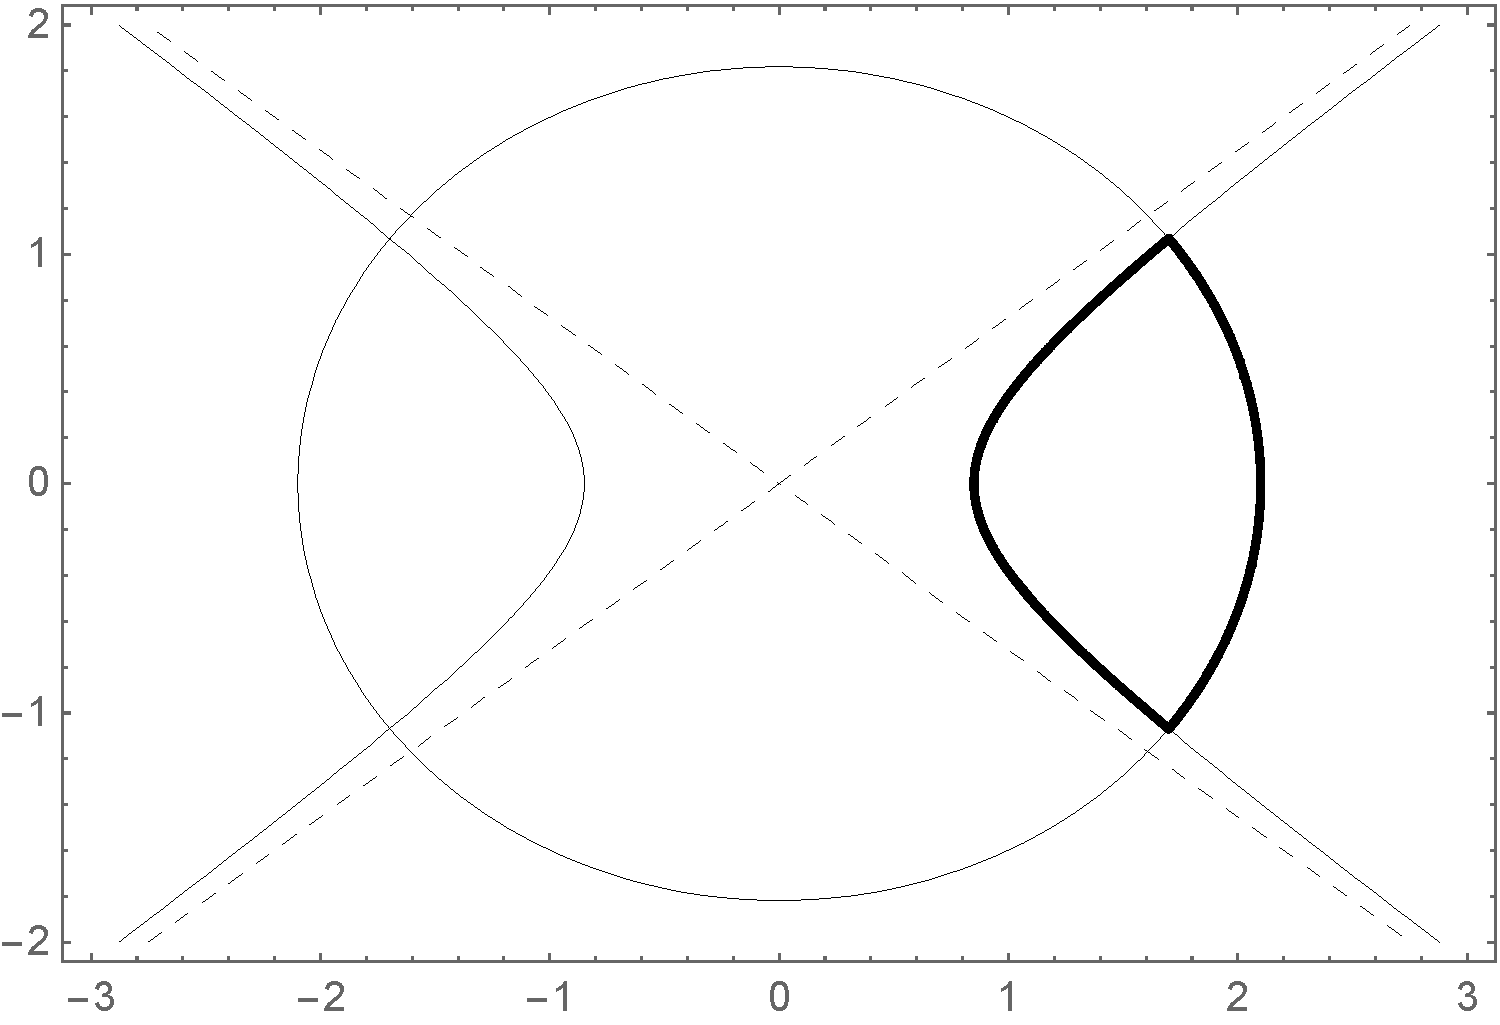
\includegraphics[width=0.8\linewidth]{right1.pdf} \\ 
        Множество $A_\varepsilon$, $\phi_0<\pi/2$
    \end{minipage}
    \hfill
    \begin{minipage}[b][][b]{0.49\linewidth}\centering
        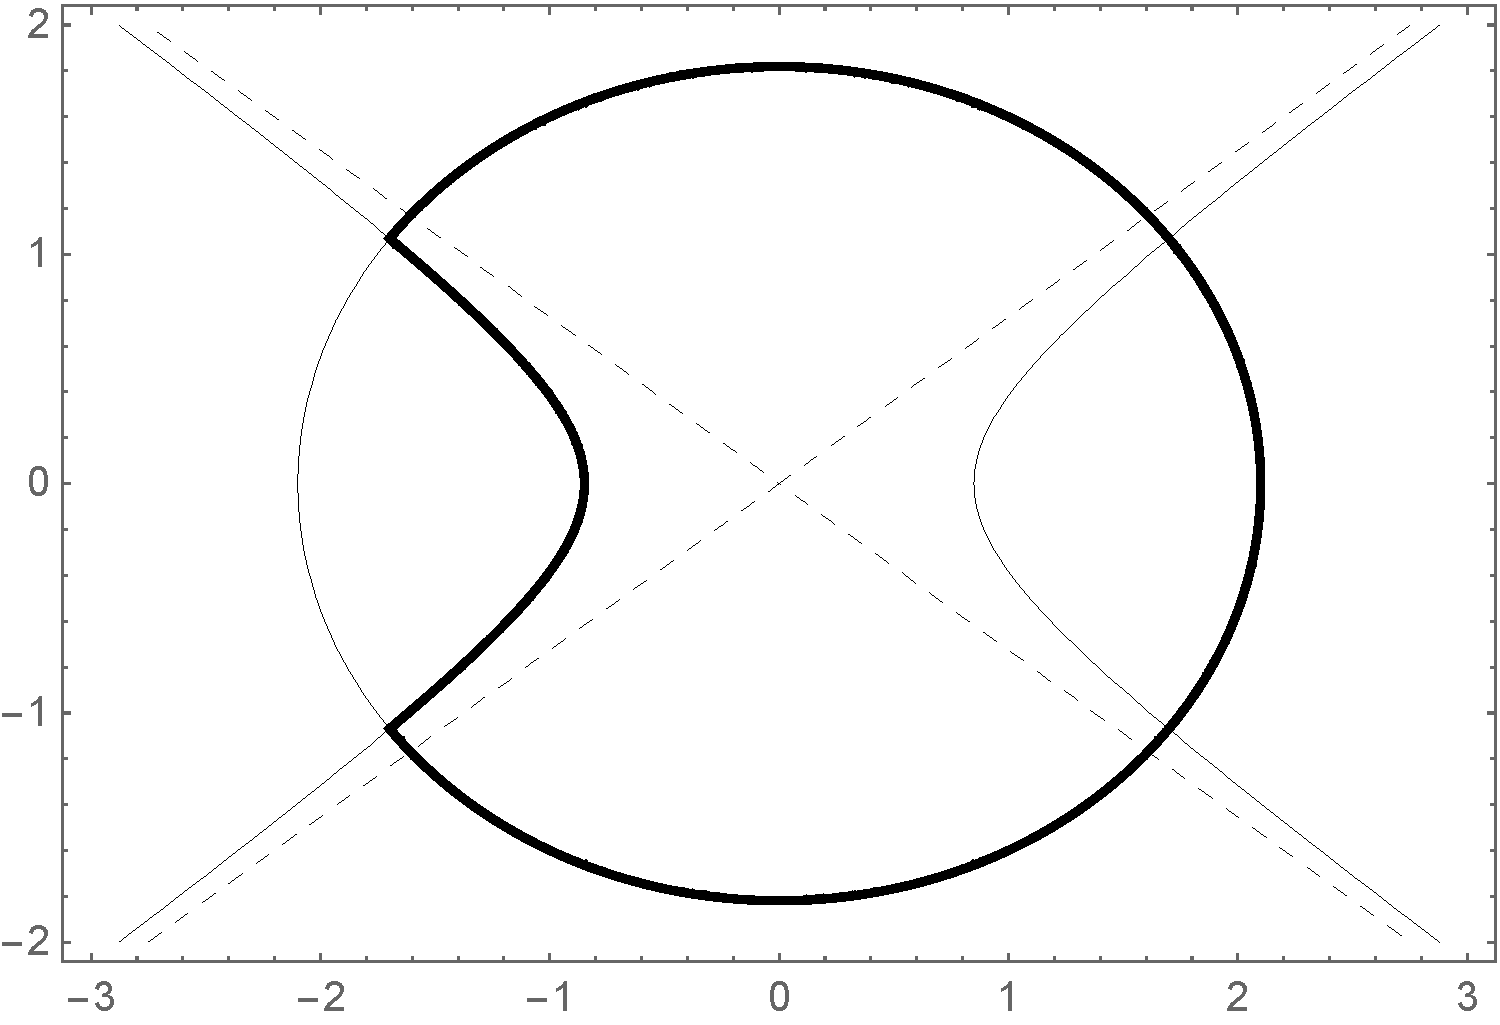
\includegraphics[width=0.8\linewidth]{left1.pdf} \\ 
        Множество $A_\varepsilon$, $\phi_0>\pi/2$
    \end{minipage}
\caption{Примеры множеств $A_\varepsilon$}
\end{figure}

\begin{figure}[ht]
\begin{minipage}{0.9\linewidth}\centering
        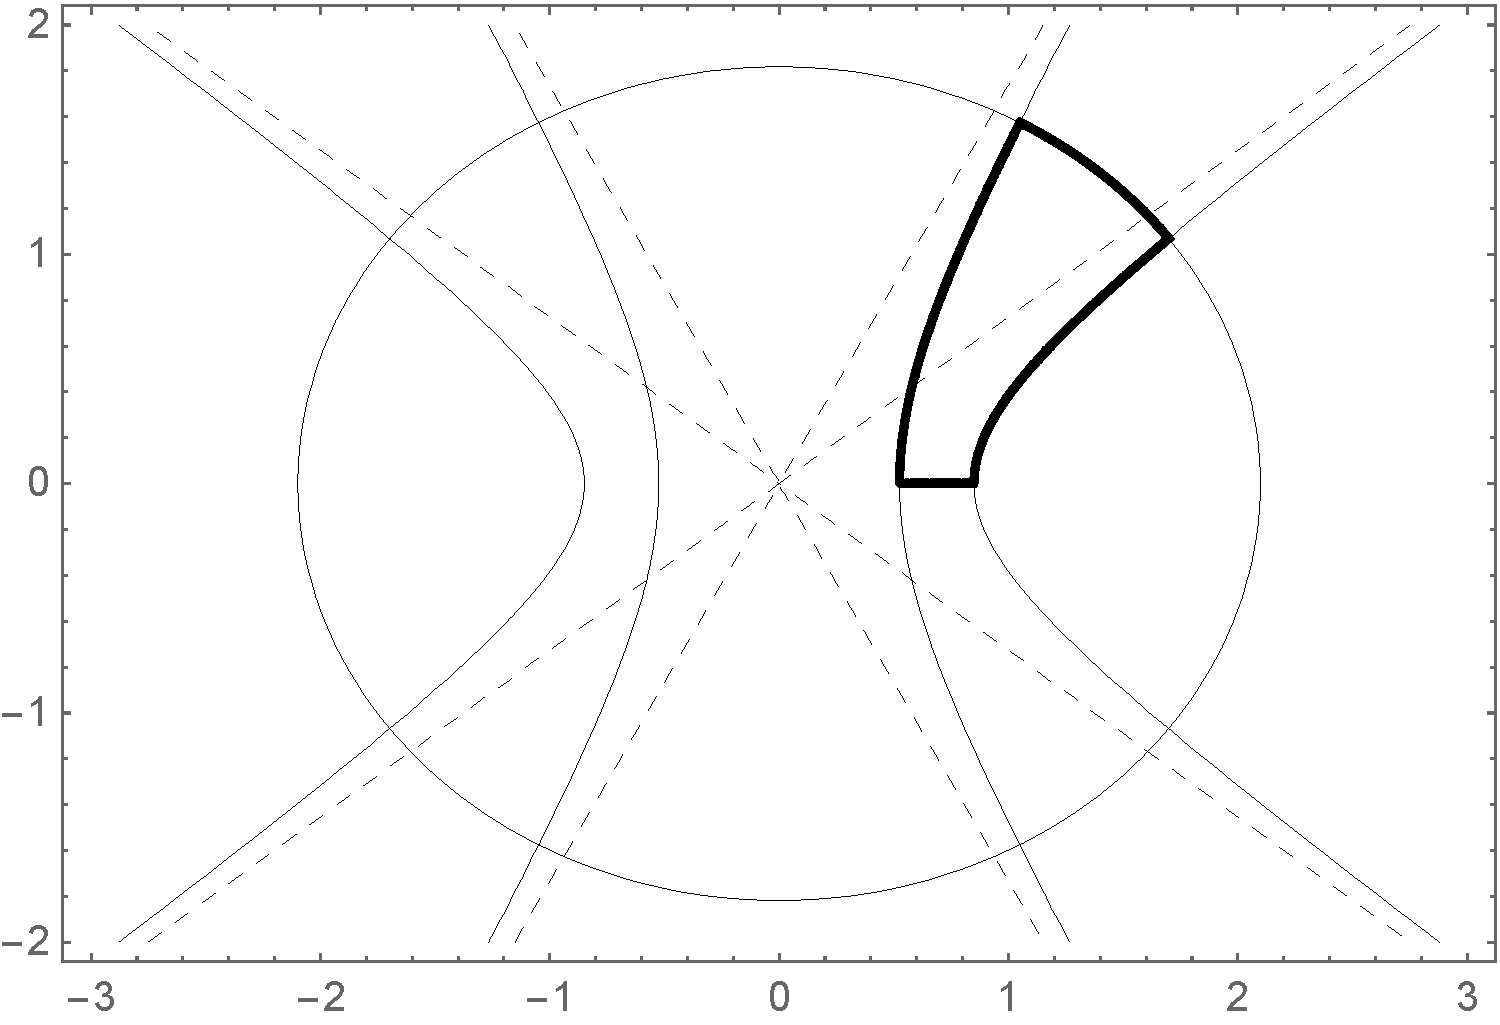
\includegraphics[width=0.8\linewidth]{up1.pdf}  
    \end{minipage}
\caption{        Множество $B_\varepsilon$, $\phi_0<\phi_1<\pi/2$}
\end{figure}

Очевидно, что с приближением величины $\varepsilon$ к 0, эллипс приближается к кругу радиуса $r_0$,
а любая гипербола~(\ref{eq:hyper}) приближается к собственным асимптотам.

Следовательно, при $\varepsilon\to 0$, область $A$ приближается к круговому сектору с величиной центрального угла $2\phi_0$, 
а область  $B$ приближается к круговому сектору с углом $\phi_1-\phi_0$. 


%\subsection{Симметричная область $A_\varepsilon: \rho \in [0,\rho_0], \phi \in [-\phi_0,\phi_0]$}\label{sec:ch2/sec2/sub2}
\subsection{Симметричная область $A_\varepsilon$}\label{sec:ch2/sec2/sub2}
\subsubsection{Собственные функции и асимптотика собственных значений}\label{sec:ch2/sec2/sub2/sub1}

Обозначим через $\Phi_{even}(\zeta, q, \phi), \Phi_{odd}(\zeta, q, \phi)$ четное и нечетное решения уравнения $\frac{\partial^2}{\partial \phi^2}\Phi + (\zeta - 2q\cos{2\phi})\Phi = 0$, соответственно. 
В частности, (см.~\cite{wref2})
\[
\begin{array}{ll}
    \Phi_{even}(a_n(q), q, \phi) = ce_n(\phi, q)	&
    \Phi_{odd}(a_n(q), q, \phi) = fe_n(\phi, q)\\
    \Phi_{even}(b_n(q), q, \phi) = ge_n(\phi, q)	&
    \Phi_{odd}(b_n(q), q, \phi) = se_n(\phi, q)\\
    \Phi_{even}(\lambda_{\nu+2k}(q), q, \phi) = ce_{\nu+2k}(\phi, q) 	&
    \Phi_{odd}(\lambda_{\nu+2k}(q), q, \phi) = se_{\nu+2k}(\phi, q).
\end{array}
\]

Напомним, что эллиптическая система координат имеет особенности на соединяющем фокусы отрезке. Область $A_\varepsilon$ содержит особые точки эллиптической системы координат, а именно, они находятся на отрезке $J$ с концами на правом фокусе и на вершине дуги гиперболы.
Следовательно, решение $\psi(\rho, \phi)$ и его производная должны удовлетворять условиям непрерывности \eqref{eq:disp} и \eqref{eq:grad} на  $J$.
В силу соображений раздела \ref{sec:ch1/sec4/sub2/sub1}, собственная функция  $\psi(\rho,\phi)=R(\rho) \Phi(\phi)$ оператора $\hat{H}$ в области $A_\varepsilon$ является произведением радиальной и угловой функций Матьё одинаковой четности:
$$ \psi(\rho,\phi) = \Phi_{even}(\phi) R_{even}(\rho)  
\text{ или }
 \psi(\rho,\phi) = \Phi_{odd}(\phi) R_{odd}(\rho) .  $$
%\hfill
%$\Box$
То есть, в наших обозначениях в области $A_\varepsilon$ для собственных функций $\psi_{k, m}(\rho, \phi)$ оператора   $\hat{H}$ справедливы выражения
\begin{equation}
\psi_{k, m}(\rho, \phi) = 
\left[
\begin{array}{ll}
    Ce_\nu(\rho, q) ce_\nu(\phi, q) ,   &    \text{нечетный $k \geq 1$}\\
    Se_\nu(\rho, q) se_\nu(\phi, q) ,   &    \text{четный $k \geq 2$}\\
\end{array}
\right.\label{eq:fun}
\end{equation}
с параметрами
\[
\nu = \nu_{k,m} = \nu_0+ \varepsilon^2 \nu_1 + o(\varepsilon^2),  \quad q=q_{k,m} = \dfrac{\varkappa_{k,m}^2 r_0^2 \varepsilon^2}{4},
\]
где
$$\nu_0 = \frac{\pi k}{2\phi_0}\text{\ \  и\  \  }\nu_1=\frac{\alpha_{\nu_0, m}^2}{4} \frac{\pi k \sin 2\phi_0}{\pi^2 k^2 - 4\phi_0^2}  .$$
Для соответствующих собственных  значений  $\varkappa^2_{k, m}$ справедливы равенства
\begin{equation}
\varkappa^2_{k, m} = \dfrac{\alpha_{\nu_0, m}^2}{r_0^2} +
\varepsilon^2 \dfrac{\alpha_{\nu_0, m}^3}{2 r_0^2}\dfrac{\varkappa_1 }{ \left.\frac{\partial J_{\nu_0}(u)}{\partial u}\right|_{u=\alpha_{\nu_0, m}} } + o(\varepsilon^2),\label{eq:val}
\end{equation}
где
\begin{equation*}
    \varkappa_1 = 
    \left[
\begin{array}{ll}
\frac{J_{\nu_0-2}(\alpha_{\nu_0, m})}{4(\nu_0-1)} - \frac{J_{\nu_0+2}(\alpha_{\nu_0, m})}{4(\nu_0+1)} 
  - \nu_1 \left.\frac{\partial J_\nu}{\partial \nu}\right|_{\nu=\nu_0}(\alpha_{\nu_0, m}),\qquad \text{для нечетных $k\geq 3$ ;} \\[10pt]
\frac{(\nu_0 - 2)J_{\nu_0-2}(\alpha_{\nu_0, m})   }{4\nu_0 (\nu_0-1)} -\\
\qquad - \frac{(\nu_0 + 2)J_{\nu_0+2}(\alpha_{\nu_0, m})}{4\nu_0 (\nu_0+1)}  
- \nu_1 \left.\frac{\partial J_\nu}{\partial \nu}\right|_{\nu = \nu_0}(\alpha_{\nu_0, m}), \qquad \ \ \!    \text{для четных $k \geq 2$}.        
\end{array}
\right.
\end{equation*}
Здесь $\alpha_{\nu_0,m}$ --  $m$-й нуль функции Бесселя первого рода $J_{\nu_0}(x)$.


Нечетный и четный случаи мы рассматриваем отдельно. Сперва рассмотрим
\textit{нечетный случай}: $\psi(\rho,\phi) = R_{odd}(\rho)\Phi_{odd}(\phi)  $.

для $\nu \in \mathbb{R} \setminus \{1\}$ 
($\nu=1$ соответствует случаю  $\phi_0=\pi$, который в работе не рассматривается)
справедливо разложение ~\cite[\S 2.2]{wref12},
\begin{align}
\Phi_{odd}(\nu, &{} \phi, q)  = \notag\\
	&{} = \sin{\nu\phi} + 
	\frac{q}{4(\nu-1)} \sin{(\nu-2)\phi} -\frac{q}{4(\nu+1)} \sin{(\nu+2)\phi} + o(q). \label{eq:se}
\end{align}
Напомним, что для $\nu \in \mathbb{R} \setminus \mathbb{Z}$, $\Phi_{odd}(\nu, \phi, q) = se_\nu(\phi, q)$ и для  $\nu \in  \mathbb{Z}$, $\Phi_{odd}(\nu, \phi, q)$ является $se_\nu(\phi, q) $ или $fe_\nu(\phi, q)$ в зависимости от $\nu$, но с тем же разложением (\ref{eq:se}). 
Поэтому, для простоты будем использовать запись $se_\nu(\phi, q)$ вместо $fe_\nu(\phi, q)$, используя только разложения с точностью до $o(q)$. Этот же подход мы будем использовать в дальнейшем без явного упоминания.

Подставим  $\phi=\phi_0$ и $\nu=\nu(q) = \nu_0 + q \nu_1 + o(q)$
в граничное условие $se_{\nu(q)}(\phi_0, q)=0$ угловой функции:
 \begin{align*}
 se_{\nu(q)}(& \phi_0, q) =  \sin \nu_0 \phi_0 + \\
&{} + q \biggl( \nu_1 \phi_0 \cos \nu_0 \phi_0 + \frac{\sin(\nu_0-2)\phi_0}{4(\nu_0-1)}  -\frac{\sin(\nu_0+2)\phi_0}{4(\nu_0+1)} \biggr) + o(q) =0.
\end{align*}
Приравнивая к нулю коэффициенты при каждой степени  $q$, мы получим
\begin{equation*}
\nu_0 = \frac{\pi (2k)}{2\phi_0}, \quad \nu_1 = \frac{\pi (2k) \sin 2 \phi_0}{(\pi^2 (2k)^2 - 4\phi_0^2)}.
\end{equation*}

Рассмотрим второе граничное условие $R(\rho_0) = 0$. 
Для функции  $R(\rho)=Se_\nu(\rho, q)$
справедливо разложение в ряд по функциям Бесселя первого рода, см.~\cite[гл. VIII]{mclachlan}, поэтому:
\begin{multline*}
Se_\nu(\rho, q) \,\propto\,\,  \nu J_\nu(2\sqrt{q} \cosh{\rho})  
+q \bigg( \frac{\nu + 2}{4(\nu+1)} J_{\nu+2}(2\sqrt{q} \cosh{\rho}) - \\
- \frac{\nu - 2}{4(\nu-1)} J_{\nu-2}(2\sqrt{q} \cosh{\rho}) \bigg) + o(q).
\end{multline*}
Символ $\propto$ означает равенство с точностью до умножения на ненулевую константу.

Заметим, что $\frac{1}{\varepsilon} = \cosh \rho = \cosh \rho_0 $, тогда из  $q = \frac{\varkappa^2 r_0^2 \varepsilon^2}{4}$ следует, что $2\sqrt{q} \cosh{\rho_0} =   \varkappa r_0$. 
Для краткости обозначим $u = \varkappa r_0$. Теперь подставим  
$\nu=\nu_0 + q\nu_1 + o(q)$ в граничное условие $0 = Se_{\nu(q)}(\rho_0, q)$:
\begin{multline*}
0 = \nu_0 J_{\nu_0}(u) + q \bigg(  \nu_1 J_{\nu_0}(u) 
- \frac{\nu_0 - 2}{4(\nu_0-1)} J_{\nu_0-2}(u) + %{} \notag\\ 
\\ %&{}+
+ \frac{\nu_0 + 2}{4(\nu_0+1)} J_{\nu_0+2}(u) +
 \nu_0 \nu_1 \left.\frac{\partial J_\nu}{\partial \nu}\right|_{\nu = \nu_0}(u)
\bigg) + o(q).
\end{multline*}
После чего подставим   $u = u_0 + q u_1 + o(q)$ в последнее равенство:
\begin{multline*}
0 = \nu_0 J_{\nu_0}(u_0) + q \bigg( 
\nu_0 u_1 \left.\frac{\partial J_{\nu_0}(u)}{\partial u}\right|_{u=u_0} 
+\nu_1 J_{\nu_0}(u_0) - \frac{\nu_0 - 2}{4(\nu_0-1)} J_{\nu_0-2}(u_0) +\\ 
+\frac{\nu_0 + 2}{4(\nu_0+1)} J_{\nu_0+2}(u_0) 
+ \nu_0 \nu_1 \left.\frac{\partial J_\nu}{\partial \nu}\right|_{\nu = \nu_0}(u_0)
\bigg) + o(q).
\end{multline*}
Снова приравнивая к $0$ коэффициенты при степенях  $q$, получим
\begin{align}
    u_0 =& \alpha_{\nu_0, m}, \label{eq:u0}\\
    u_1 =& \frac{1}{\left.\frac{\partial J_{\nu_0}(u)}{\partial u}\right|_{u=\alpha_{\nu_0, m}} } \biggl(
\frac{(\nu_0 - 2)J_{\nu_0-2}(\alpha_{\nu_0, m}) }{4 \nu_0(\nu_0-1)} - \notag \\    
&{}- \frac{(\nu_0 + 2)J_{\nu_0+2}(\alpha_{\nu_0, m}) }{4 \nu_0(\nu_0+1)} - \nu_1 \left.\frac{\partial J_\nu}{\partial \nu}\right|_{\nu = \nu_0}(\alpha_{\nu_0, m})
    \biggr),\label{eq:u1}
\end{align}
где $\alpha_{\nu_0, m}$ --  $m$-й нуль функции Бесселя $J_{\nu_0}(x)$. 




Из равенства $q=\frac{\varkappa^2 r_0^2 \varepsilon^2}{4}=\frac{u^2 \varepsilon^2}{4}$ можно получить выражение для собственного значения
$$\varkappa_{k, m}^2 = \frac{u^2}{r_0^2} = \frac{u_0^2}{r_0^2} + \frac{2 q u_0 u_1}{r_0^2} + o(q)= \frac{u_0^2}{r_0^2} +  \varepsilon^2 \frac{u_0^3 u_1}{2 r_0^2} + o(\varepsilon^2).$$ 
Из уравнений~(\ref{eq:u0}) и (\ref{eq:u1}) для $u_0, u_1$ верны выражения
\begin{align}
  & \nu_0 = \frac{2\pi k}{2\phi_0},   \nu_1 = \frac{2 \pi k \sin 2 \phi_0}{4 k^2\pi^2  - 4\phi_0^2},\\
   & \varkappa_{k, m}^2 = \frac{\alpha_{\nu_0, m}^2}{r_0^2} 
+  \varepsilon^2 \frac{\alpha_{\nu_0, m}^3}{2 r_0^2}\frac{1}{ \left.\frac{\partial J_{\nu_0}(u)}{\partial u}\right|_{u=\alpha_{\nu_0, m}} } \biggl(
\frac{(\nu_0 - 2)J_{\nu_0-2}(\alpha_{\nu_0, m})   }{4\nu_0 (\nu_0-1)} - \notag \\
&\qquad\qquad{}- \frac{(\nu_0 + 2)J_{\nu_0+2}(\alpha_{\nu_0, m})}{4\nu_0 (\nu_0+1)} - \nu_1 \left.\frac{\partial J_\nu}{\partial \nu}\right|_{\nu = \nu_0}(\alpha_{\nu_0, m})
    \biggr) + o(\varepsilon^2).
 \label{eq:oddSe_nueigenvalues}
 \end{align}


Теперь рассмотрим случай  $\psi(\phi, \rho) = \Phi_{even}(\phi) R_{even}(\rho)$ с \textit{четными} функциями $ \Phi_{even}(\phi) $ и $R_{even}(\rho)$. 
В силу аналогичных соображений, рассмотрим разложение четного решения:
\[
ce_\nu(\phi, q) = 	\cos{\nu\phi} + 
	\frac{q}{4(\nu-1)} \cos{(\nu-2)\phi} -\frac{q}{4(\nu+1)} \cos{(\nu+2)\phi} + o(q).
\]
Используя равенство $ce_\nu(\phi_0, q)=0$ и разложение $\nu = \nu_0 + q \nu_1 + o(q)$,
запишем разложение $ce_\nu$  по степеням $q$:
\begin{multline*}
0=ce_\nu(\phi_0, q) = 	\cos{\nu_0\phi_0}  + \\
+q \biggl(	\frac{\cos{(\nu_0-2)\phi_0}}{4(\nu_0-1)}  -\frac{\cos{(\nu_0+2)\phi_0}}{4(\nu_0+1)} - \nu_1 \phi_0 \sin \nu_0 \phi_0 \biggr) + o(q).
 \end{multline*}
Приравнивая к  $0$ коэффициенты при различных степенях  $q$, получаем
\begin{equation*}
    \nu_0 = \frac{\pi (1 + 2 k)}{2 \phi_0}, \qquad \nu_1 = \frac{\pi (1+2k) \sin 2\phi_0}{\pi^2(1+2k)^2 - 4\phi_0^2}.
\end{equation*}

Чтобы вывести формулу для  $\varkappa^2$, рассмотрим граничное условие $R(\rho_0) = 0$. 
Поскольку $R(\rho) = Ce_\nu(\rho, q)$, можно воспользоваться разложением в сумму по функциям Бесселя первого рода:
\begin{align*}
Ce_\nu(\rho, q) = & J_\nu(2\sqrt{q} \cosh{\rho}) + {}\notag \\
&{}+q \biggl( \frac{1}{4(\nu+1)} J_{\nu+2}(2\sqrt{q}\cosh{\rho}) -\frac{1}{4(\nu-1)} J_{\nu-2}(2\sqrt{q} \cosh{\rho})
\biggr) + o(q).
\end{align*}
Заметим, что $\frac{1}{\varepsilon} = \cosh \rho = \cosh \rho_0 $, тогда из  $q = \frac{\varkappa^2 r_0^2 \varepsilon^2}{4}$ следует, что $2\sqrt{q} \cosh{\rho_0} =   \varkappa r_0$. 
Обозначим для краткости $u = \varkappa r_0$. 

Подставим  $\nu = \nu_0 + q \nu_1 + o(q)$  в граничное условие $0 = Ce_{\nu(q)}(\rho_0, q)$:
\begin{equation}
    0 = 
    J_{\nu_0}(u) + q \biggl( 
    \frac{J_{\nu_0+2}(u)}{4(\nu_0+1)}  - \frac{J_{\nu_0-2}(u)}{4(\nu_0-1)}
    + \nu_1 \left.\frac{\partial J_\nu}{\partial \nu}\right|_{\nu=\nu_0}(u)
    \biggr) + o(q).\label{eq:evenae}
\end{equation}
Теперь подставим $u = u_0 + q u_1 + o(q)$  в полученное выражение~(\ref{eq:evenae}):
\begin{align*}
    &0 =  Ce_{\nu(q)}(\rho_0, q) = 
    J_{\nu_0}(u_0) + q \biggl( 
    u_1 \left.\frac{\partial J_{\nu_0} (u)}{\partial u}\right|_{u=u_0} +  \notag \\
  &\quad{}  + \frac{J_{\nu_0+2}(u_0)}{4(\nu_0+1)} - \frac{J_{\nu_0-2}(u_0)}{4(\nu_0-1)}    + \nu_1 \left.\frac{\partial J_\nu}{\partial \nu}\right|_{\nu=\nu_0}(u_0)
    \biggr) + o(q).
\end{align*}
Из равенства $0$ коэффициентов при каждой степени $q$ следует
\begin{align*}
&u_0 = \alpha_{\nu_0, m}, \\
&u_1 = \frac{1}{\left.\frac{\partial J_{\nu_0} (u)}{\partial u}\right|_{u=\alpha_{\nu_0, m}}} 
\biggl(
\frac{J_{\nu_0-2}(\alpha_{\nu_0, m})}{4(\nu_0-1)} - \frac{J_{\nu_0+2}(\alpha_{\nu_0, m})}{4(\nu_0+1)}
 - \nu_1 \left.\frac{\partial J_\nu}{\partial \nu}\right|_{\nu=\nu_0}(\alpha_{\nu_0, m})
\biggr),
\end{align*}
где $\alpha_{\nu_0, m}$ -- $m$-й нуль функции $J_{\nu_0}(x)$.  

Как и в предыдущем случае, собственное значение
$$\varkappa_{k, m}^2 = \frac{u^2}{r_0^2} = \frac{u_0^2}{r_0^2} + \varepsilon^2 \frac{u_0^3 u_1}{2r_0^2} + o(\varepsilon^2)$$ получается подстановкой значений $u_0, u_1$:
\begin{align*}
&\nu_0 = \frac{\pi (1 + 2 k)}{2 \phi_0}, \quad \nu_1 = \frac{\pi (1+2k) \sin 2\phi_0}{\pi^2(1+2k)^2 - 4\phi_0^2},\\
&\varkappa_{k, m}^2 = \frac{\alpha_{\nu_0, m}^2}{r_0^2} + \varepsilon^2 \frac{\alpha_{\nu_0, m}^3}{2r_0^2} \frac{1}{\left.\frac{\partial J_{\nu_0} (u)}{\partial u}\right|_{u=\alpha_{\nu_0, m}}}\biggl(
\frac{J_{\nu_0-2}(\alpha_{\nu_0, m})}{4(\nu_0-1)} - \notag\\
&\qquad{} - \frac{J_{\nu_0+2}(\alpha_{\nu_0, m})}{4(\nu_0+1)}    - \nu_1 \left.\frac{\partial J_\nu}{\partial \nu}\right|_{\nu=\nu_0}(\alpha_{\nu_0, m})
\biggr) + o(\varepsilon^2).
\end{align*}

\subsubsection{Особый случай: $A_\varepsilon$ для $\phi_0=\pi/2$}\label{sec:ch2/sec2/sub2/sub1}


Для $\nu\ne 1$ формулы для собственных функций и собственных значений, см. уравнения (\ref{eq:fun}) и (\ref{eq:val}), верны. Единственным исключением является случай  $\nu=\nu_0=1$.
Для $\nu=\nu_0=1$ для четного решения справедливо разложение (см. \cite[Subsect.~20.2.27]{wref2}):
\begin{equation*}
ce_1(\phi, q) = 	\cos{\phi}  - \frac{q}{8} \cos{3\phi} + o(q),
 \end{equation*}
для которого граничное условие  $ce_1(\phi_0, q)=0$ выполняется. 
Рассмотрим второе граничное условие $R(\rho_0) = 0$.
Для $R(\rho) = Ce_1(\rho, q)$ существует разложение по функциям Бесселя первого рода:
\begin{equation*}
Ce_1(\rho, q) = J_1(2\sqrt{q} \cosh{\rho}) + \frac{q}{8} J_3(2\sqrt{q}\cosh{\rho}) + o(q).
\end{equation*}
Из подстановок $\cosh\rho = \cosh\rho_0 =  \frac{1}{\varepsilon}$ и $q = \frac{\varkappa^2 r_0^2 \varepsilon^2}{4}$ следует равенство
$2\sqrt{q} \cosh{\rho_0} = 2 \frac{\varkappa r_0 \varepsilon}{2} \frac{1}{\varepsilon} = \varkappa r_0$. Для краткости $\varkappa r_0$ обозначим через $u$. 

Подставим $\nu = 1$ в граничное условие $0 = Ce_1(\rho_0, q)$ и рассмотрим разложение в ряд по степеням   $q$:
\begin{equation*}
    0 = J_1(u) + q \left( \frac{J_3(u)}{8} \right) + o(q).
\end{equation*}
Подстановкой  $u = u_0 + q u_1 + o(q)$ получим:
\begin{equation*}
    0 = 
    J_1(u_0) + q \left( 
    u_1 \left.\frac{\partial J_1 (u)}{\partial u}\right|_{u=u_0}
    + \frac{J_3(u_0)}{8}
    \right) + o(q).
\end{equation*}
Поэтому, 
\begin{equation*}
u_0 = \alpha_{1, m}, \qquad u_1 = 
\frac{ - J_3(\alpha_{1, m}) }{8\left.
\frac{\partial J_1 (u)}{\partial u}\right|_{u=\alpha_{1, m}}},
\end{equation*}
где $\alpha_{1, m}$ -- $m$-й нуль функции Бесселя  $J_1(x)$. По аналогии с предыдущим случаем,
собственное значение $\varkappa_{k, m}^2 = \frac{u^2}{r_0^2} = \frac{u_0^2}{r_0^2} + \varepsilon^2 \frac{u_0^3 u_1}{2r_0^2} + o(\varepsilon^2)$ получается из подстановки величин  $u_0, u_1$:
\begin{align}
   & \varkappa_{k, m}^2 = \frac{\alpha_{1, m}^2}{r_0^2} - \varepsilon^2 \frac{\alpha_{1, m}^3}{16r_0^2} 
    \frac{J_3(\alpha_{1, m})}{\left.\frac{\partial J_1 (u)}{\partial u}\right|_{u=\alpha_{1, m}}} 
    + o(\varepsilon^2), \label{eq:valS1}
    \end{align}



%\subsection{Несимметричная область $B_\varepsilon:  \rho \in [0, \rho_0], \phi \in [\phi_0, \phi_1 ]$}\label{sec:ch2/sec2/sub3}
\subsection{Несимметричная область $B_\varepsilon$}\label{sec:ch2/sec2/sub3}
\subsubsection{Собственные функции и асимптотика собственных значений}\label{sec:ch2/sec2/sub3/sub1}


Внутренность области $B_\varepsilon$ не содержит особых точек эллиптической системы координат~(\ref{eq:coord}). Поэтому, условия непрерывности сдвига или непрерывности производной, рассмотренные для случая симметричной области (в частности, для эллипса), здесь не требуются.
Хотя эти особые точки, тем не менее, появятся на границе  $B_\varepsilon$ (а именно, они образуют горизонтальный отрезок в составе границы).

Рассмотрим собственную функцию $\psi_{k,l}(\rho,\phi) = R(\rho)\Phi(\phi)$.
Обращение  $\psi_{k,l}(\rho,\phi) $ в нуль на горизонтальном отрезке на границе  $B_\varepsilon$
подразумевает, что $\psi_{k,l}(\rho,\phi)$ может быть представлена в виде
\[
\psi(\rho,\phi) = 
    \left(
    \Phi_{even}(\phi_0) \Phi_{odd}(\phi) - \Phi_{even}(\phi) \Phi_{odd}(\phi_0) 
    \right) R_{odd}(\rho).
\]

%{\em Далее следует основной результат текущего подраздела.}
В области  $B_\varepsilon$ для собственных функций $\psi_{k, m}(\rho, \phi)$ и собственных значений $\varkappa^2_{k, m}$ оператора $\hat{H}$ справедливы выражения

\begin{align}
&\psi_{k, m}(\rho, \phi) = 
    Se_\nu(\rho, q) \biggl( ce_\nu(\phi_0, q) se_\nu(\phi, q) -ce_\nu(\phi, q) se_\nu(\phi_0, q) \biggr) ,  \label{eq:funB}
\end{align}
с параметрами
\begin{align*}    
    & q=q_{k,m} = \frac{\varkappa_{k,m}^2 r_0^2 \varepsilon^2}{4}, \\ 
&\nu = \nu_{k,m} = \frac{\pi k}{\phi_1-\phi_0} +\varepsilon^2 \frac{\alpha_{\nu_0, m}^2}{4} \frac{\pi k (\sin 2\phi_1 - \sin 2 \phi_0)}{\pi^2k^2-(\phi_1-\phi_0)^2} + o(\varepsilon^2) ,  
\end{align*}
где
\begin{align*}
& \nu_0 = \frac{\pi k}{\phi_1-\phi_0},\text{\ \ и \ \ }
\nu_1= \frac{\pi k (\sin 2\phi_1 - \sin 2 \phi_0)}{\pi^2k^2-(\phi_1-\phi_0)^2} .
\end{align*}
Для соответствующих собственных значений справедливы равенства
\begin{align}
\varkappa_{k, m}^2 ={}& \frac{\alpha_{\nu_0, m}^2}{r_0^2} +  \varepsilon^2 \frac{\alpha_{\nu_0, m}^3}{2 r_0^2}\frac{1}{ \left.\frac{\partial J_{\nu_0}(u)}{\partial u}\right|_{u=\alpha_{\nu_0, m}} }  
 \biggl(\frac{(\nu_0 - 2)J_{\nu_0-2}(\alpha_{\nu_0, m})   }{4\nu_0 (\nu_0-1)} -
\notag \\ 
&{}- \frac{(\nu_0 + 2)J_{\nu_0+2}(\alpha_{\nu_0, m})}{4\nu_0 (\nu_0+1)} 
- \nu_1 \left.\frac{\partial J_\nu}{\partial \nu}\right|_{\nu = \nu_0}(\alpha_{\nu_0, m})
    \biggr) + o(\varepsilon^2).\label{eq:valB}
\end{align}
Здесь $\alpha_{\nu_0,m}$ -- $m$-й нуль функции Бесселя первого рода $J_{\nu_0}(x)$.


Мы хотим найти решение углового решения в виде
\begin{multline*}
\Phi(\phi, q) = \Phi_{even}(\phi_0) \Phi_{odd}(\phi) - \Phi_{even}(\phi) \Phi_{odd}(\phi_0)  = \\
=ce_\nu(\phi_0, q) se_\nu(\phi, q) - ce_\nu(\phi, q) se_\nu(\phi_0, q).
\end{multline*}

 
Подстановим $\nu(q) = \nu_0 + q \nu_1 + o(q)$
в граничное условие  $\Phi(\phi_1, q) = 0$
и из разложения функций $ce_\nu(\phi, q)$ и $se_\nu(\phi, q)$, в ряды по степеням  $q$
 получим
\begin{multline*}
0=\Phi(\phi_1, q) = ce_\nu(\phi_0, q) se_\nu(\phi_1, q) -ce_\nu(\phi_1, q) se_\nu(\phi_0, q) = \\
= \sin \nu_0 (\phi_1 - \phi_0) +q \biggl(
\frac{1}{4(\nu_0+1)}  \sin{(2 \phi_0 + \nu_0(\phi_0-\phi_1))}+  \\
+\frac{1}{4(\nu_0+1)} \sin{(\nu_0(\phi_0-\phi_1)-2\phi_1)} - \\
-\frac{1}{2(\nu_0-1)}\cos{(\phi_0 + \phi_1)}\sin{(\nu-1)(\phi_0-\phi_1)} -\\
- \nu_1 (\phi_0 - \phi_1) \cos{\nu_0(\phi_0-\phi_1)} \biggr) + o(q).
\end{multline*}
Следовательно, 
\begin{equation*}
    \nu_0 = \frac{\pi k}{\phi_1-\phi_0}, \qquad \nu_1 = \frac{\pi k (\sin 2\phi_1 - \sin 2 \phi_0)}{\pi^2k^2-(\phi_1-\phi_0)^2}.
\end{equation*}

Из соображений, аналогичных тем, что были проведены для  $\psi_{k, m}(\rho, \phi) = \Phi_{odd}(\phi) R_{odd}(\rho)$ из предыдущего подраздела,
мы получаем разложение радиальной функции и соответствующих собственных значений:
\begin{align*}
    \varkappa_{k, m}^2 ={}& \frac{\alpha_{\nu_0, m}^2}{r_0^2} +  \varepsilon^2 \frac{\alpha_{\nu_0, m}^3}{2 r_0^2}\frac{1}{ \left.\frac{\partial J_{\nu_0}(u)}{\partial u}\right|_{u=\alpha_{\nu_0, m}} }\biggl(\frac{(\nu_0 - 2)J_{\nu_0-2}(\alpha_{\nu_0, m})   }{4\nu_0 (\nu_0-1)} - \notag \\
&{}- \frac{(\nu_0 + 2)J_{\nu_0+2}(\alpha_{\nu_0, m})}{4\nu_0 (\nu_0+1)}  - \nu_1 \left.\frac{\partial J_\nu}{\partial \nu}\right|_{\nu = \nu_0}(\alpha_{\nu_0, m})
    \biggr) + o(\varepsilon^2).
\end{align*}

\subsubsection{Особые случаи: $B_\varepsilon$ для $(\phi_0, \phi_1)=(0,\pi)$ и для $(\phi_0, \phi_1)=(0,\pi/2)$}\label{sec:ch2/sec2/sub3/sub2}


Хотя $\phi_0=0, \phi_1=\pi/2$ является особенным случаем при $k=1$,
несложно проверить, что уравнения (\ref{eq:funB}) и (\ref{eq:valB}) выполняются.

Для  $\phi_0=0, \phi_1=\pi$
особенным является случай  $k=1$ (следовательно, $\nu_0=1$). 
Для остальных величин $k$ равенства (\ref{eq:funB}) и (\ref{eq:valB}) справедливы.
Теперь предположим $k=1$ (и $\nu=\nu_0 = 1$).
Тогда для соответствующего нечетного решения углового уравнения справедливо разложение  (см. \cite[Subsect.~20.2.27]{wref2})
\begin{equation*}
se_1(\phi, q) = 	\sin{\phi}  - 	\frac{q}{8} \sin{3\phi} + o(q),
 \end{equation*}
для которого выполняется граничное условие $se_1(\phi_0, q)=0$. 
Теперь рассмотрим второе граничное условие $R(\rho_0) = 0$. 
Для функции $R(\rho) = Se_1(\rho, q)$ справедливо разложение по функциям Бесселя первого рода:
\begin{equation*}
Se_1(\rho, q) = J_1(2\sqrt{q} \cosh{\rho}) + \frac{3 q}{8} J_3(2\sqrt{q}\cosh{\rho}) + o(q).
\end{equation*}
Подставим $\cosh \rho = \cosh \rho_0 =\frac{1}{\varepsilon}$.
Тогда из $q = \frac{\varkappa^2 r_0^2 \varepsilon^2}{4}$ следует равенство
$2\sqrt{q} \cosh{\rho_0} =  \varkappa r_0$.

Для краткости положим $u = \varkappa r_0$ .
Подставим $\nu = 1$ в граничное условие радиальной функции и разложим ее в ряд степенной ряд по $q$:
\begin{equation*}
    0 = Se_1(\rho_0, q) = 
    J_1(u) + q  \frac{3 J_3(u)}{8} + o(q).
\end{equation*}
Теперь подставим $u = u_0 + q u_1 + o(q)$:
\begin{align*}
    0 = Se_1(\rho_0, q) =    J_1(u_0) + q \left( 
    u_1 \left.\frac{\partial J_1 (u)}{\partial u}\right|_{u=u_0}
    + \frac{3 J_3(u_0)}{8}
    \right) + o(q).
\end{align*}
Отсюда 
\begin{equation*}
u_0 = \alpha_{1, m}, \qquad u_1 = 
\frac{ - 3 J_3(\alpha_{1, m}) }{8\left.
\frac{\partial J_1 (u)}{\partial u}\right|_{u=\alpha_{1, m}}},
\end{equation*}
где $\alpha_{1, m}$ -- $m$-й нуль функции $J_1(x)$. 

Наконец, как в предыдущем случае, подстановкой $u_0, u_1$ в $\varkappa_{1, m}^2 = \frac{u^2}{r_0^2} = \frac{u_0^2}{r_0^2} + \varepsilon^2 \frac{u_0^3 u_1}{2r_0^2} + o(\varepsilon^2)$, получим выражение для собственного значения:
\begin{align}
    \varkappa_{1, m}^2& = \frac{\alpha_{1, m}^2}{r_0^2} - \varepsilon^2 \frac{3\alpha_{1, m}^3}{16r_0^2} 
    \frac{J_3(\alpha_{1, m})}{\left.\frac{\partial J_1 (u)}{\partial u}\right|_{u=\alpha_{1, m}}} 
    + o(\varepsilon^2).  \label{eq:valS2}
\end{align}



\FloatBarrier
           % Глава 2
\chapter{Эллиптический бильярд с косинусным законом преломления на софокусных квадриках.}\label{ch:ch3}

\section{Предварительные сведения.}\label{sec:ch3/sec1}

\subsection{Классический бильярд.}\label{sec:ch3/sec1/sub1}

Зафиксируем большую и малую полуоси эллипса $a$ и $b$, где $a > b > 0$ и во внутренности эллипса $\left(f(x, y) = \dfrac{x^2}{a^2}+\dfrac{y^2}{b^2} < 1 \right)$ рассмотрим движение материальной точки с координатами $\mathbf{x} = (x, y)$ и вектором скорости $\mathbf{v} = (v_x, v_y)$, при котором на границе эллипса $f(x, y) = 1$ векторы скорости до отражения и после него образуют равные по величине углы с вектором нормали $n=\left.\nabla f(x,y)\right|_{(x_0,y_0)} = \left( \dfrac{2x_0}{a^2},\dfrac{2y_0}{b^2}\right)$ к эллипсу в точке отражения $(x_0, y_0)$.

Обозначим $\Psi = \left\{ Q_{\lambda} \ |\ \lambda \in (0, a^2) \right\}$ -- однопараметрическое семейство софокусных квадрик, где квадрика $Q_\lambda$ задается уравнением 
$$f_\lambda(x,y)=\dfrac{x^2}{a^2-\lambda} + \dfrac{y^2}{b^2-\lambda} = 1.$$

Интегрируемость классического бильярда обусловлена классической теоремой из геометрии: если какое-то звено бильярдной траектории коснулось софокусной квадрики $Q_\lambda$ из семейства $\Psi$, то и все остальные звенья касаются этой же квадрики, поэтому $\lambda$ является первым интегралом.


\subsection{Интеграл Иоахимсталя.}\label{sec:ch3/sec1/sub2}
Пусть $M = Q_0 \times \mathbb{R}^2$ -- фазовый цилиндр бильярда в эллипсе $Q_0$. Для точки $(\mathbf{x}, \mathbf{v}) = ((x,y), (v_x, v_y)) \in M$ рассмотрим функцию $J(\mathbf{x}, \mathbf{v}) = -\left(
\frac{x v_x}{a^2} + \frac{y v_y}{b^2} \right).$
Функция $J(\mathbf{x}, \mathbf{v})$ не является интегралом движения точки в эллиптическом бильярде, так как не сохраняется на прямолинейных отрезках траектории. Тем не менее, для <<дискретного>> бильярда в эллипсе, когда траектория записывается последовательностью точек на эллипсе, в которых траектории испытывают отражения, функция $J(\mathbf{x}, \mathbf{v})$ является интегралом. А именно, прямолинейное звено бильярдной траектории будем кодировать начальной точкой звена $(x, y)$ и его вектором скорости $(v_x, v_y)$. Тогда выполняется следующее утверждение: 

\begin{theorem}{\normalfont{[7, с.~61]}}.
Пусть $(\mathbf{x}_i, \mathbf{v}_i) \in M, \quad i=1,\ldots$, -- последовательность точек на фазовом цилиндре, кодирующая последовательные звенья некоторой  бильярдной траектории. Тогда $J(\mathbf{x}_i, \mathbf{v}_i) =  J(\mathbf{x}_{i+1}, \mathbf{v}_{i+1})$ для всех $i$.
\label{th:sect3_th1}
\end{theorem}

Функцию $J$ называют интегралом Иоахимсталя. Заметим, что эту функцию можно переписать в виде 
$$J(\mathbf{x}, \mathbf{v}) = -\frac{1}{2}\langle\mathbf{v}, \nabla f_0(x, y)\rangle,$$
где $\langle\cdot, \cdot\rangle$ обозначает скалярное произведение. 

Прежде чем перейти к геометрическому смыслу интеграла Иоахимсталя, рассмотрим следующий вопрос: сколько квадрик из семейства $\Psi = \left\{ Q_{\lambda} \ |\ \lambda \in (0, a^2) \right\}$ касаются   фиксированной произвольным образом прямой в $\mathbb{R}^2$?

\begin{statement}
Рассмотрим прямую $\mathbf{x}+t\mathbf{v}$, проходящую через точку $\mathbf{x}= (x, y)$ на плоскости $\mathbb{R}^2$ и имеющую направление $\mathbf{v}=(v_x, v_y)$. Тогда:

$(i)$ Прямая касается не более одной квадрики $Q_\lambda$ из семейства $\Psi$.

$(ii)$ Исключая вертикальную ось $x=0$ и прямые, проходящие хотя бы через один из фокусов,  такая касательная квадрика  $Q_\lambda$ существует и ее параметр $\lambda$ определяется по формуле 
\begin{equation}
\lambda = \Lambda(\mathbf{x}, \mathbf{v}) = \frac{a^2 v_y^2 + b^2v_x^2 - (x v_y-y v_x)^2}{v_x^2 + v_y^2}.
\label{eq:sect3_eq1}
\end{equation}

\end{statement}

\begin{proof}
Прямая $\mathbf{x} + t \mathbf{v}$ касается квадрики $Q_\lambda$ тогда и только тогда, когда уравнение
$$\frac{(x + t v_x)^2}{a^2-\lambda} + \frac{(y + t v_y)^2}{b^2-\lambda} = 1$$
имеет ровно одно решение по $t$, то есть когда дискриминант квадратного уравнения с переменной $t$  равен нулю. Приравнивая дискриминант к нулю и решая равенство относительно параметра софокусной квадрики $\lambda$ можно получить формулу \eqref{eq:sect3_eq1} из второго пункта формулировки утверждения. В случаях, если $\lambda = a^2$ или $\lambda = b^2$, касательная квадрика $Q_\lambda$ вырождается в прямую (проходящую через малую полуось при $\lambda = a^2$ и проходящая через большую полуось при $\lambda = b^2$), следовательно прямая $\mathbf{x}+ t\mathbf{v}$ не касается никакой софокусной квадрики $Q_\lambda$.
\end{proof}

Заметим, что для бильярда в эллипсе вычисленный в точке $(\mathbf{x}, \mathbf{v})$ фазового цилиндра $M$ интеграл Иоахимсталя связан с параметром софокусной квадрики $\lambda$, которой касается прямая с направляющим вектором $\mathbf{v}$, проходящая через точку $\mathbf{x}$.

\begin{statement}
    Пусть $(\mathbf{x}, \mathbf{v})$ кодируют некоторое звено бильярдной траектории. Пусть $\lambda$ -- параметр квадрики $Q_\lambda$, касающейся прямой $\mathbf{x} +t \mathbf{v}$. Тогда 
    \begin{equation}
        \lambda = \Lambda(\mathbf{x}, \mathbf{v}) =  a^2 b^2 \frac{J^2(\mathbf{x}, \mathbf{v})}{||\mathbf{v}||^2}
    \label{eq:sect3_eq2}
    \end{equation}
\end{statement}

\begin{proof}
Выражение \eqref{eq:sect3_eq1} для $\lambda$ перепишем, домножив обе части на знаменатель:
\begin{equation}
(v_x^2 + v_y^2)\lambda = a^2 v_y^2 + b^2v_x^2 - (x v_y-y v_x)^2 = (a^2-x^2)v_y^2 + (b^2-y^2)v_x^2 + 2 x y v_x v_y.
\label{eq:sect3_eq3}
\end{equation}
Точка $(x, y)$ находится на эллипсе $Q_0$, поэтому
\begin{equation}
a^2 - x^2 = \frac{a^2 y^2}{b^2} \text{  и } b^2 - y^2 = \frac{b^2 x^2}{a^2}.
\label{eq:sect3_eq4}
\end{equation}
Подставляя \eqref{eq:sect3_eq4} в \eqref{eq:sect3_eq3}, получаем
$$||\mathbf{v}||^2 \lambda = \frac{a^2y^2}{b^2} + \frac{b^2 x^2}{a^2} + 2 x y v_x v_y = ||\mathbf{v}||^2 a^2b^2 \left( \frac{x v_x}{a^2} + \frac{y v_y}{b^2}\right)^2 = a^2b^2J^2(\mathbf{x}, \mathbf{v}).$$
\end{proof}

\section{Косинусный закон преломления.}\label{sec:ch3/sec2}
Пусть две области $\Omega_i$ и $\Omega_j$ граничат по кривой $C$. 
Показатели преломления для этих областей равны $n_i$ и $n_j$, соответственно.
Будем считать, что движение материальной точки при достижении кривой $C$ подчиняется следующим правилам (далее мы будем ссылаться на них как на модифицированный закон преломления $(\ast)$).
\begin{itemize}
\item[1.] Выполнено соотношение $n_i \cos \theta_i = n_j \cos \theta_j $, где $\theta_i, \theta_j \in [0,\frac{\pi}{2} ]$ -- углы, которые образуют отрезки траектории   в соответствующих областях с нормалью к кривой $C$, если $\theta_i$ и $\theta_j$ корректно определены.
\item[2.] Если $n_i > n_j$ и материальная точка, двигаясь в области $\Omega_i$, достигает кривой $C$, причем в точке пересечения траектории с кривой $C$ выполнено неравенство $\cos \theta_i > \frac{n_j}{n_i}$, то происходит полное внутреннее отражение траектории в область $\Omega_i$ по закону <<угол падения равен углу отражения>> (в этом случае угол $\theta_j$ не определен, поскольку $\frac{n_i}{n_j} \cos \theta_i > 1$). 
\item[3.] В предыдущих двух пунктах два соседних отрезка траектории с общей точкой на кривой $C$ лежат по разные стороны от нормали к кривой $C$ в этой точке.
\item[4.] Если $n_i > n_j$ и материальная точка, двигаясь в области $\Omega_j$, достигает кривой $C$, причем $\theta_j = 0$, тогда $\cos \theta_i = \frac{n_j}{n_i}$ и материальная точка продолжает движение в области $\Omega_i$ вдоль любого из двух возможных направлений, образующих угол $\theta_i$ с нормалью к кривой $C$.
\item[5.] Аналогично при $n_i < n_j$.
\end{itemize}
Для удобства будем считать, что при преломлении модуль вектора скорости не меняется.

\begin{figure}[!htb]
\minipage{0.32\textwidth}
\includegraphics[width=\linewidth]{images/ch4/section1/example1.pdf}
    \caption{Иллюстрация к пункту 1.}
    \label{fig:pt8:_example1}
\endminipage\hfill
\minipage{0.32\textwidth}
\includegraphics[width=\linewidth]{images/ch4/section1/example2.pdf}
    \caption{Иллюстрация к пункту 2.}
    \label{fig:pt8:_example2}
\endminipage\hfill
\minipage{0.32\textwidth}
\includegraphics[width=\linewidth]{images/ch4/section1/example3.pdf}
    \caption{Иллюстрация к пункту 4.}
    \label{fig:pt8:_example3}
\endminipage\hfill
\end{figure}

\subsection{Постоянная движения}\label{sec:ch3/sec3}
Пусть задана область $\Omega$, ограниченная эллипсом 
$\dfrac{x^2}{a^2} + \dfrac{y^2}{b^2} = 1$, где $a > b > 0$.
Дуга софокусной квадрики $Q_{\lambda_0} = \left\{ \dfrac{x^2}{a^2-\lambda_0} + \dfrac{y^2}{b^2-\lambda_0} = 1 \right\}$ разделяет  $\Omega$ на области $\Omega_1$ и $\Omega_2$.
В случае $0 < \lambda_0 < b^2$ квадрика $Q_{\lambda_0}$ является эллипсом, а при $b^2 < \lambda_0 < a^2$ -- гиперболой.

Припишем каждой области $\Omega_i$  коэффициент $n_i,\  i=1,2$, имеющий смысл показателя преломления. 
Рассмотрим движение материальной точки в области $\Omega$. Будем считать, что на внешней границе области $\Omega$ движение подчиняется закону <<угол падения равен углу отражения>>, 
а на общей границе областей $\Omega_1$ и $\Omega_2$ выполняется модифицированный закон преломления $(\ast)$.

Определим функцию $\Xi(x, y, v_x, v_y)$ положения и скорости материальной точки (в декартовых координатах) по формуле
\begin{equation}
\Xi(x, y, v_x, v_y) = \left[
\begin{array}{ll}
    \Lambda(x, y, v_x, v_y) n_1^2, &  \text{ если } (x,y) \in \Omega_1 \\
    \Lambda(x, y, v_x, v_y) n_2^2 + \lambda_0 (n_1^2-n_2^2), & \text{ если } (x,y) \in \Omega_2    .
\end{array}
\right.
\label{eq:xi_integral_definition}
\end{equation}
Здесь величина $\Lambda(x, y, v_x, v_y)$ определена как в уравнении \eqref{eq:sect3_eq1} и имеет смысл коэффициента $\alpha$  софокусной квадрики $Q_\alpha$, которая касается прямой, проходящей через точку $(x,y)$ в направлении вектора $(v_x, v_y)$.

Функция $\Xi(x, y, v_x, v_y)$ является первым интегралом рассматриваемой динамической системы в области $\Omega$.
Доказательство изложено в разделе \ref{sec:ch3/sec3/sub2}.

\subsubsection{Вспомогательные утверждения}\label{sec:ch3/sec3/sub1}

 \begin{statement}
Пусть $\mathbf{n}$ -- вектор нормали разделяющей среды кривой $C$ в точке преломления $(x_0, y_0)$, а также пусть $\mathbf{v}$ -- вектор скорости до преломления. Считаем, что траектория бильярда в точке $(x_0, y_0)$ переходит из среды с показателем преломления $n_1$ в область с показателем $n_2$. Тогда если вектор $\mathbf{v}$ не параллелен вектору $\mathbf{n}$, то для вектора   $\mathbf{w}$  после преломления справедливо выражение 
$\mathbf{w} = \alpha \mathbf{v} + \beta \mathbf{n}$, где 
$$\beta = \dfrac{||\mathbf{w}|| \mu - ||\mathbf{v}|| \alpha}{||\mathbf{n}||}\cos{\theta_1}, \ \alpha = \dfrac{||\mathbf{w}||}{||\mathbf{v}||}\sqrt{\dfrac{1-\mu^2\cos^2 \theta_1}{1-\cos^2 \theta_1 }},$$  $\theta_1$ -- угол, образованный векторами $\mathbf{v}$ и $\mathbf{n}$, $\mu = \dfrac{n_1}{n_2}$.
\label{st:alpha_beta_cosine_law}
\end{statement}
\begin{proof}
Из закона преломления $(\ast)$ следует 
$\langle\mathbf{w}, \mathbf{n}\rangle = ||\mathbf{w}||\, ||\mathbf{n}|| \cos \theta_2 = ||\mathbf{w}||\, ||\mathbf{n}|| \mu \cos \theta_1$.

В то же время, из линейности скалярного произведения
$\langle\mathbf{w}, \mathbf{n}\rangle = \alpha \langle\mathbf{v}, \mathbf{n}\rangle + \beta\, ||\mathbf{n}||^2 = \alpha ||\mathbf{v}||\, ||\mathbf{n}|| \cos \theta_1 + \beta\, ||\mathbf{n}||^2$, следовательно, $\beta = \dfrac{||\mathbf{w}|| \mu - ||\mathbf{v}|| \alpha}{||\mathbf{n}||}\cos{\theta_1}$. 

Подставляя полученное значение $\beta$ в равенство $||\mathbf{w}||^2 = ||\alpha \mathbf{v} + \beta \mathbf{n}||^2 = \alpha^2 ||\mathbf{v}||^2 (1-\cos^2 \theta_1) + \mu^2||\mathbf{w}||^2 \cos^2 \theta_1$, получим нужную формулу для  $\alpha$.
\end{proof}

\begin{remark}
    Эти формулы очевидным образом упрощаются для $||\mathbf{n}|| = 1$ и $||\mathbf{v}|| = ||\mathbf{w}||$. В дальнейшем мы будем использовать эти формулы при $||\mathbf{v}|| = ||\mathbf{w}||$, но $||\mathbf{n}|| \neq 1$.
\end{remark}

\begin{statement}
Если траектория подходит к границе раздела сред $Q_{\lambda_0}$ под прямым углом (т.е. вектор скорости $\mathbf{v}$ пропорционален вектору нормали $\mathbf{n}$   квадрики $Q_{\lambda_0}$ в точке преломления $(x_0,y_0)$) и коэффициенты преломления не дают полное отражение (то есть $n_1 \cos \theta_1 = n_1 \leq n_2$), то вектор скорости после преломления может быть определен предельным переходом:
\begin{multline*}
\dfrac{\mathbf{w}}{||\mathbf{w}||} - \mu \dfrac{\mathbf{n}}{||\mathbf{n}||}=  \sqrt{\dfrac{1-\mu^2 \cos^2 \theta_1 }{1-\cos^2\theta_1}} \left( \dfrac{\mathbf{v}}{||\mathbf{v}||} - \dfrac{\mathbf{n}}{||\mathbf{n}||} \right) = \\
=  \sqrt{\dfrac{1-\mu^2 \cos^2 \theta_1 }{\sin^2\theta_1}}  \left(
    \begin{array}{cc}
    \cos \theta_1 - 1 \ & -\sin \theta_1 \\
    \sin \theta_1 \ & \cos \theta_1 - 1 
    \end{array}
\right) \dfrac{\mathbf{n}}{||\mathbf{n}||} = \\
=  \sqrt{1-\mu^2 \cos^2 \theta_1 }  \left(
    \begin{array}{cc}
    -\tan \frac{\theta_1}{2}  \ & -1 \\
    1 \ & -\tan \frac{\theta_1}{2}
    \end{array}
\right) \dfrac{\mathbf{n}}{||\mathbf{n}||} \ \xrightarrow[\theta_1 \to 0+]{} \ 
\sqrt{1-\mu^2}  \left(
    \begin{array}{cc}
    0  \ & -1 \\
    1  \ & 0
    \end{array}
\right) \dfrac{\mathbf{n}}{||\mathbf{n}||},
\end{multline*}
что эквивалентно пункту 4 закона $(\ast)$.
\end{statement}


\begin{statement}
Рассмотрим точку $\mathbf{x}=(x, y) \in Q_{\lambda_0}$ и пару векторов скоростей $\mathbf{v}$, $\mathbf{w}$ до и после преломления в точке $\mathbf{x}$, соответственно. 
Имеет место равенство
\begin{equation}
\dfrac{n_2 J_{\lambda_0}(\mathbf{x}, \mathbf{w})}{||\mathbf{w}||} = 
\dfrac{n_1 J_{\lambda_0}(\mathbf{x}, \mathbf{v})}{||\mathbf{v}||}.
\label{eq:sect3_eq7}
\end{equation}
%$\frac{J_{\lambda_0}(\mathbf{x}, \mathbf{w})}{||\mathbf{w}||} = \mu \frac{J_{\lambda_0}(\mathbf{x}, \mathbf{v})}{||\mathbf{v}||}$
\label{th:joachFraction}
\end{statement}

%\begin{remark}
%Мы записали основное равенство в этом утверждении именно в такой форме, чтобы  была очевидна связь с формулой \eqref{eq:sect3_eq2} для $\Lambda(\mathbf{x}, \mathbf{v})$.
%\end{remark}
\begin{proof}
Из определения функции $J_{\lambda_0}$ следует равенство $J_{\lambda_0}(\mathbf{x}, \mathbf{v}) = -\frac{1}{2}||\mathbf{v}|| ||\mathbf{n}|| \cos \theta_1$, а с учетом формул для коэффициентов $\alpha$ и $\beta$ из утверждения \ref{st:alpha_beta_cosine_law} получаем 
\begin{multline*}
    J_{\lambda_0}(\mathbf{x}, \mathbf{w}) = \alpha J_{\lambda_0}(\mathbf{x}, \mathbf{v}) + \beta J_{\lambda_0}(\mathbf{x}, \mathbf{n}) = \alpha J_{\lambda_0}(\mathbf{x}, \mathbf{v}) - \frac{\beta}{2}||\mathbf{n}||^2 = \\ =\alpha J_{\lambda_0}(\mathbf{x}, \mathbf{v}) + ||\mathbf{n}||^2\frac{||\mathbf{w}||\mu-||\mathbf{v}||\alpha}{||\mathbf{n}||}\frac{J_{\lambda_0}(\mathbf{x}, \mathbf{v})}{||\mathbf{v}|| ||\mathbf{n}||} = 
\frac{||\mathbf{w}||}{||\mathbf{v}||}\mu J_{\lambda_0}(\mathbf{x}, \mathbf{v}),
\end{multline*}
где $\mu=\frac{n_1}{n_2}$. Следовательно, 
$
\frac{n_2 J_{\lambda_0}(\mathbf{x}, \mathbf{w})}{||\mathbf{w}||} = 
\frac{n_1 J_{\lambda_0}(\mathbf{x}, \mathbf{v})}{||\mathbf{v}||}.
$
\end{proof}

\begin{statement}
    
    $(i)$ При $\theta_1=0$ и $n_1 \leq n_2$ равенство
    \eqref{eq:sect3_eq7} тоже выполняется 
    
    $(ii)$ Более того, величины $J_{\lambda_0}(\mathbf{x}, \mathbf{w})$ для <<левой>> и <<правой>> траекторий совпадают.
\end{statement}
\begin{proof}

$(i)$ Поскольку $\mathbf{v} \| \mathbf{n}$, $||\mathbf{w}|| = ||\mathbf{v}||$,  то очевидно равенство 
    $$J_{\lambda_0}(\mathbf{x}, \mathbf{w}) 
    = -\frac{1}{2}||\mathbf{n}||||\mathbf{w}|| \cos \theta_2 
    = -\frac{1}{2}||\mathbf{n}||||\mathbf{v}|| \cos \arccos \frac{n_1}{n_2} 
    = \frac{n_1}{n_2} J_{\lambda_0}(\mathbf{x}, \mathbf{v}).$$

$(ii)$ В силу четности косинуса из определения $J_{\lambda_0}(\mathbf{x}, \mathbf{w})$ следует, что
\begin{multline*}
J_{\lambda_0}(\mathbf{x}, R(\theta_2) \mathbf{v})
=-\frac{1}{2}\langle\mathbf{n},  R(\theta_2) \mathbf{v}\rangle
=-\frac{1}{2}||\mathbf{n}||||\mathbf{v}|| \cos \theta_2 = \\
=-\frac{1}{2}||\mathbf{n}||||\mathbf{v}|| \cos -\theta_2 
=-\frac{1}{2}\langle\mathbf{n},  R(-\theta_2) \mathbf{v}\rangle
=J_{\lambda_0}(\mathbf{x}, R(-\theta_2) \mathbf{v}).
\end{multline*}
\end{proof}

\subsubsection{Постоянная движения $\Xi$ (доказательство)}\label{sec:ch3/sec3/sub2}
Вернемся к системе, описанной в разделе \ref{sec:ch3/sec3}.
\begin{theorem}
    Функция $\Xi(\mathbf{x}, \mathbf{v})$, определенная как в уравнении \eqref{eq:xi_integral_definition}, является постоянной на траекториях для бильярда с законом преломления $(\ast)$.
\label{th:xi_is_integral}
\end{theorem} 
\begin{proof}


Очевидно, что функция $\Xi(\mathbf{x}, \mathbf{v})$ является константой на каждом отрезке бильярдной траектории с преломлением, полностью лежащем в $\Omega_1$ или $\Omega_2$. Легко сообразить, что в момент отражения функция $\Xi(\mathbf{x}, \mathbf{v})$ также не меняет своего значения. Остается рассмотреть  момент преломления. С геометрической точки зрения удобно воспользоваться функцией  
$$J_{\lambda_0}(\mathbf{x}, \mathbf{v}) = -\left(\frac{x v_x}{a^2-\lambda_0} + \frac{y v_y}{b^2-\lambda_0} \right) = -\frac{1}{2}\langle\mathbf{v}, \nabla f_{\lambda_0}(x,y)\rangle,$$
определенной на дуге $\partial \Omega_1 \cap \partial \Omega_2$ квадрики $Q_{\lambda_0}$, заданной уравнением $f_{\lambda_0}(x, y) = 1$.

На дуге  $\partial \Omega_1 \cap \partial \Omega_2$ имеет место равенство
 $$\Lambda(\mathbf{x}, \mathbf{v})=(a^2-\lambda_0)(b^2-\lambda_0)\frac{J_{\lambda_0}(\mathbf{x}, \mathbf{v})^2}{||\mathbf{v}||^2}.$$

Рассмотрим траекторию бильярда в момент преломления. Для определенности предположим, что  до преломления частица движется в среде с коэффициентом преломления $n_1$ с вектором скорости $\mathbf{v}$, который меняется на вектор $\mathbf{w}$ после перехода в среду с коэффициентом преломления $n_2$. При движении в обратном порядке эти два звена меняются местами, а нижеследующие утверждения по-прежнему справедливы.

Сначала рассмотрим каустику для области, коэффициент преломления которой равен $n_1$: пусть $(x,y) \in Q_{\lambda_0}$ и прямая $\mathbf{x}+t \mathbf{v}$ касается квадрики с параметром $\alpha_1$. 


Перепишем выражение для $\Lambda$ (см. \eqref{eq:sect3_eq1}) эквивалентным способом:
\begin{equation}
\alpha_1 = \Lambda(\mathbf{x}, \mathbf{v}) = \frac{(a^2-x^2) v_y^2 + (b^2-y^2)v_x^2 +2 x y v_x v_y}{v_x^2 + v_y^2}.
\label{eq:sect3_eq8}
\end{equation}
Из условия $(x,y) \in Q_{\lambda_0}$, т.е. из равенства $\frac{x^2}{a^2-\lambda_0} + \frac{y^2}{b^2-\lambda_0} =1$, используя соотношения \eqref{eq:sect3_eq4}, получаем:
$$a^2-x^2=\frac{a^2-\lambda_0}{b^2-\lambda_0}y^2+\lambda_0 \ \text{ и }\  b^2-y^2 = \frac{b^2-\lambda_0}{a^2-\lambda_0}x^2+\lambda_0.$$
Подставим эти выражения в формулу \eqref{eq:sect3_eq8} для $\alpha_1$:
\begin{multline*}
\alpha_1 = \frac{\frac{a^2-\lambda_0}{b^2-\lambda_0}y^2v_y^2 + \lambda_0 v_y^2 + \frac{b^2-\lambda_0}{a^2-\lambda_0}x^2v_x^2 + \lambda_0 v_x^2 + 2x y v_x v_y}{v_x^2+v_y^2} = \\
=\lambda_0 + (a^2-\lambda_0)(b^2-\lambda_0)\dfrac{(\frac{x v_x}{a^2-\lambda_0} + \frac{y v_y}{b^2-\lambda_0})^2}{v_x^2 + v_y^2} = 
\lambda_0 + (a^2-\lambda_0)(b^2-\lambda_0)\frac{J_{\lambda_0}(\mathbf{x}, \mathbf{v})^2}{||\mathbf{v}||^2}.
\end{multline*}

Повторяя те же рассуждения для преломленного луча $\mathbf{w}$, для параметра каустики $\alpha_2 = \Lambda(\mathbf{x}, \mathbf{w})$ имеем 
\begin{equation}
\alpha_2 = \lambda_0 + (a^2-\lambda_0)(b^2-\lambda_0)\frac{J_{\lambda_0}(\mathbf{x}, \mathbf{w})^2}{||\mathbf{w}||^2} = \lambda_0 + (a^2-\lambda_0)(b^2-\lambda_0)\frac{J_{\lambda_0}(\mathbf{x}, \mathbf{v})^2}{||\mathbf{v}||^2} \left(\frac{n_1}{n_2}\right)^2.
\label{eq:sect3_eq9}
\end{equation}

В результате из равенств \eqref{eq:sect3_eq8} и \eqref{eq:sect3_eq9} следует, что $\Lambda(\mathbf{x}, \mathbf{v}) - \lambda_0 = (\Lambda(\mathbf{x}, \mathbf{w}) - \lambda_0)\left(\frac{n_2}{n_1}\right)^2$. 
\end{proof}


\section{Общий случай}\label{sec:ch3/sec3}
Утверждение теоремы \ref{th:xi_is_integral} для $\Xi(\mathbf{x}, \mathbf{v})$ оказывается верным в значительно более общей ситуации.
Пусть внутренность эллипса разбита попарно непересекающимися дугами софокусных квадрик на области $\Omega_1, \ldots, \Omega_k$.  Перенумеруем области так, чтобы общие границы имели только области с соседними номерами. Пусть $\lambda_j$ --- параметр софокусной квадрики, разделяющей $\Omega_j$ и $\Omega_{j+1}$, $j=1, \ldots, k-1$. Два возможных варианта показаны на рис. \ref{fig:pt8:_example4} и \ref{fig:pt8:_example5}. Здесь и далее показатель преломления для области $\Omega_j$ обозначается через $n_j$.
\begin{figure}[!htb]
\minipage{0.45\textwidth}
   \includegraphics[width=1\textwidth]{images/ch4/section1/multiple ellipses.pdf}
    \caption{Взаимное расположение областей $\Omega_1, \ldots, \Omega_k$.}
    \label{fig:pt8:_example4}
\endminipage\hfill
\minipage{0.45\textwidth}
    \includegraphics[width=0.9\textwidth]{images/ch4/section1/multiple hyperbolas.pdf}   
    \caption{Взаимное расположение областей $\Omega_1, \ldots, \Omega_k$.}
    \label{fig:pt8:_example5}
\endminipage\hfill
\end{figure}


Определим функцию $\Xi(x, y, v_x, v_y)$ по формуле: 
\begin{equation*}
\Xi(x, y, v_x, v_y) = \left[
\begin{array}{ll}
    \Lambda(x, y, v_x, v_y) n_1^2, \qquad  \ \ \qquad   \text{ если } (x,y) \in \Omega_1 ;
    \\
    \Lambda(x, y, v_x, v_y) n_p^2 + \sum_{j=1}^{p-1} \lambda_j(n_j^2-n_{j+1}^2), \\
     \qquad \qquad \qquad \qquad \qquad \qquad  \text{ если } (x,y) \in \Omega_p \text{ для } 1 < p \leq k. 
\end{array}
\right.
\end{equation*}

\begin{theorem}[\cite{vestnikLatest}]
Функция $\Xi(x, y, v_x, v_y)$ является константой на траекториях бильярда с модифицированным законом  преломления
\end{theorem}
Доказательство этого утверждения полностью аналогично доказательству теоремы \ref{th:xi_is_integral}.

Таким образом, возникает следующая важная естественная задача.

\textbf{Задача А:} описать слоение изоэнергетического многообразия на поверхности уровня первого интеграла $\Xi$ для случаев, показанных на рис. \ref{fig:pt8:_example4} и \ref{fig:pt8:_example5}. 

В работе подробно рассматривается случай двух областей, разделенных одним софокусным эллипсом (см. рис. \ref{fig:pt8:_example4} при $k=2$). Динамика этой системы и перестройки поверхностей постоянного значения интеграла $\Xi$ уже в этом случае очень нетривиальны.
\bigskip

Случаи, когда область $\Omega$ разбивается на подобласти дугами \textit{пересекающихся} софокусных квадрик, оказываются гораздо сложнее. В частности, дополнительный интеграл принимает значения не в $\mathbb{R}$, а в фактор-группе $\mathbb{R}$ по  аддитивной подгруппе, допускающей явное описание.


\textit{ Случай 1: одна точка пересечения. }

\begin{figure}[!htb]
\centering
     \includegraphics[width=0.35\textwidth]{images/ch4/section1/img2.pdf}
\caption{Взаимное расположение областей $\Omega_1,\ldots,\Omega_4$.}
    \label{fig:pt8:_example6}
\end{figure}

Предположим, что внутренность эллипса разделена на области дугами софокусных квадрик таким образом, что имеются всего одна точка их пересечения, которую обозначим $A$.
Занумеруем области против часовой стрелки $\Omega_1, \ \Omega_2, \ \Omega_3, \ \Omega_4$ (см. рис. \ref{fig:pt8:_example6}).
Пусть общая часть границы $\Omega_1 \cup \Omega_4$ и $\Omega_2 \cup \Omega_3$ --- дуга софокусной квадрики с параметром $\lambda_1$, а общая часть границы $\Omega_1 \cup \Omega_2$ и $\Omega_3 \cup \Omega_4$ --- дуга софокусной квадрики с параметром $\lambda_2$ (см. рис. \ref{fig:pt8:_example6}).

Введем коэффициент $\gamma_A$ в точке $A$, имеющий смысл коэффициента ветвления, по формуле $$\gamma_A = \lambda_1(n_1^2 - n_2^2) + \lambda_2(n_2^2-n_3^2) + \lambda_1(n_3^2-n_4^2) + \lambda_2(n_4^2-n_1^2) = (\lambda_1 - \lambda_2) ( n_1^2 - n_2^2 + n_3^2 - n_4^2).$$

Определим вспомогательную функцию $\widetilde{\Xi}(x, y, v_x, v_y)$ 

\begin{equation*}
\widetilde{\Xi}(x, y, v_x, v_y) = \left[
\begin{array}{ll}
    \Lambda(x, y, v_x, v_y) n_1^2, \qquad  \  \ \qquad   \text{ если } (x,y) \in \Omega_1 
    \\
    \Lambda(x, y, v_x, v_y) n_p^2 + \sum_{j=1}^{p-1} \lambda_j(n_j^2-n_{j+1}^2), \\
     \qquad \qquad \qquad \qquad \qquad \qquad  \text{ если } (x,y) \in \Omega_p \text{ для } 1 < p \leq 4. 
\end{array}
\right.
\end{equation*}
Неформально говоря, она почти подходит на роль дополнительного интеграла, но имеет разрыв на дуге, разделяющей области $\Omega_1$ и $\Omega_4$. Можно проверить, что на любой бильярдной траектории, пересекающей эту дугу, функция $\widetilde{\Xi}$ испытывает один и тот же скачок, равный  $\pm \gamma_A$. 
Поэтому мы определим \textit{первый интеграл $\Xi(x, y, v_x, v_y)$ со значениями в $S^1= \mathbb{R}/\gamma_A \mathbb{Z}$ }по формуле $$\Xi(x, y, v_x, v_y) = \widetilde{\Xi}(x, y, v_x, v_y) \mod \gamma_A.$$
Эта величина на траекториях бильярда сохраняется.
\bigskip

Если границы раздела областей пересекаются по двум и более точкам, то имеет место общая закономерность: 
\medskip

\textit{ 
\noindent Для каждой точки пересечения $A_i, i=1,\ldots,m$, определен коэффициент $\gamma_{A_i}$. Дополнительный интеграл \  $\Xi(x, y, v_x, v_y)$ принимает значения в $\mathbb{R}/(\gamma_{A_1} \mathbb{Z}+ \ldots + \gamma_{A_m} \mathbb{Z})$. Если $\gamma_{A_i}$ соизмеримы, т. е. всевозможные дроби $\dfrac{\gamma_{A_i}}{\gamma_{A_j}}$ --- рациональные числа (или бесконечность), то $\mathbb{R}/(\gamma_{A_1} \mathbb{Z}+ \ldots + \gamma_{A_m} \mathbb{Z}) = S^1$. Если же среди $\gamma_{A_i}$ есть пара с иррациональным отношением $\dfrac{\gamma_{A_i}}{\gamma_{A_j}}$, то подгруппа $\gamma_{A_1} \mathbb{Z}+ \ldots + \gamma_{A_m} \mathbb{Z}$ всюду плотна в $\mathbb{R}$. В этом случае дополнительный интеграл $\Xi(x, y, v_x, v_y)$ корректно определен, но использовать его для топологического анализа структуры траекторий представляется весьма затруднительным.}

\bigskip
\textit{ Случай 2: две точки пересечения.}
\begin{figure}[!htb]
\centering
   \includegraphics[width=0.35\textwidth]{images/ch4/section1/img3.pdf}   
    \caption{Взаимное расположение областей $\Omega_1, \ldots, \Omega_4$.}
    \label{fig:pt8:_example7}
\end{figure}
Рассмотрим области, изображенные на рис. \ref{fig:pt8:_example7}. 
Легко вычислить коэффициенты $\gamma_{A_1}$ и $\gamma_{A_2}$ в точках $A_1, A_2$ (т.е. скачки дополнительного интеграла при обходе против часовой стрелки вокруг соответствующей точки):
$$\gamma_{A_1} = \lambda_2(n_1^2 - n_4^2) + \lambda_1(n_4^2-n_3^2) + \lambda_2(n_3^2-n_2^2) + \lambda_1(n_2^2-n_4^2), $$
% = (\lambda_2 - \lambda_1) ( n_1^2 - n_2^2 + n_3^2 - n_4^2),$$
$$\gamma_{A_2} = \lambda_1(n_1^2 - n_2^2) + \lambda_2(n_2^2-n_3^2) + \lambda_1(n_3^2-n_4^2) + \lambda_2(n_4^2-n_1^2). $$
% = (\lambda_1 - \lambda_2) ( n_1^2 - n_2^2 + n_3^2 - n_4^2).$$
Как видно, в этом случае $$\gamma_{A_1} = -\gamma_{A_2}.$$
Поэтому дополнительный интеграл $\Xi(x, y, v_x, v_y)$, сохраняющийся на траекториях бильярда, может быть задан по модулю $\gamma_{A_1}$ формулой $\Xi = \widetilde{\Xi} \mod \gamma_{A_1}$, где 
\begin{equation*}
\widetilde{\Xi}(x, y, v_x, v_y) = \left[
\begin{array}{ll}
    \Lambda(x, y, v_x, v_y) n_1^2,  \qquad \ \  \qquad  \text{ если } (x,y) \in \Omega_1 
    \\
    \Lambda(x, y, v_x, v_y) n_p^2 + 
    \sum_{j=1}^{p-1} \lambda_j(n_j^2-n_{j+1}^2), \\
     \qquad \qquad  \qquad \qquad  \qquad \qquad \text{ если } (x,y) \in \Omega_p \text{ для } 1 < p \leq 4. 
\end{array}
\right.
\end{equation*}
 \medskip
\textit{ Случай 3: две точки пересечения.}
Рассмотрим области, изображенные на рис. \ref{fig:pt8:_example8}. 
\begin{figure}[!htb]
\centering
   \includegraphics[width=0.35\textwidth]{images/ch4/section1/img4.pdf}   
    \caption{Взаимное расположение областей $\Omega_1, \ldots, \Omega_6$.}
    \label{fig:pt8:_example8}
\end{figure}


Легко видеть, что коэффициенты $\gamma_{A_1}, \gamma_{A_2}$ в точках $A_1$, $A_2$, соответственно, задаются формулами:
$$\gamma_{A_1} = (\lambda_3 - \lambda_1)(n_2^2 - n_5^2 + n_6^2 - n_3^2),$$
$$\gamma_{A_2} = (\lambda_3 - \lambda_2)(n_1^2 - n_4^2 + n_5^2 - n_2^2).$$

В зависимости от значений параметров отношение $\dfrac{\gamma_{A_1}}{\gamma_{A_2}}$ может быть как рациональным, так и иррациональным.

Роль коэффициента $\gamma_A$ проявляется в следующей задаче, которую мы решим в рамках настоящей статьи.

\textbf{Задача Б.} Рассмотрим в качестве бильярдной области $\Omega$  <<прямоугольник>>, образованный дугами концентрических окружностей $BC$, $AD$ и отрезками вертикально проведенного диаметра $AB$ и $CD$. (см. рис. \ref{fig:pt8:_example9}).
Область $\Omega$ разбивается на две части дугой  $EF$ концентрической окружности  и отрезком $FG$ горизонтально проведенного диаметра. Нумерация областей показана на рис. \ref{fig:pt8:_example9}.

Требуется описать как изоэнергетическое многообразие расслаивается на поверхности уровня первого интеграла $\Xi$.


\begin{figure}[!htb]
\centering
   \includegraphics[width=0.25\textwidth]{images/ch4/section1/imgB.pdf}   
    \caption{Взаимное расположение областей $\Omega_1, \Omega_2$.}
    \label{fig:pt8:_example9}
\end{figure}

%Перечислим основные результаты настоящей работы.
%Для задачи А полностью описаны поверхности уровня регулярных значений интеграла $\Xi$ (теорема \ref{st:pt9:n1_n2_surfaces}).
%В разделе \ref{sec:ch4/sec2/subsec2} описаны поверхности уровня для всех нерегулярных значений интеграла $\Xi$, а также все перестройки поверхностей уровня интеграла при проходе через сингулярные значения. 
%Для задачи Б  показано, что многозначный интеграл $\Xi$ в действительности принимает лишь конечное число значений, в теоремах \ref{th:pt10:th1} и \ref{th:pt10:th2} и подразделе \ref{sec:ch4/sec3/subsec8} полностью описаны поверхности уровня регулярных значений интеграла $\Xi$.
%Описанию особых слоев и перестроек посвящен подраздел \ref{sec:ch4/sec3/subsec10}.

\clearpage
           % Глава 3
\section{Введение}\label{s1}
Теория интегрируемых бильярдов развивается в двух в каком-то смысле встречных направлениях:

(1) доказательство гипотезы Биркгофа; 

(2) поиск интегрируемых модификаций эллиптического бильярда.

В решении задачи (1), начиная с работы С.~В.~Болотина \cite{Bol90}, за последние годы был достигнут значительный прогресс --- упомянем здесь работы Миронова, Бялого и Драговича \cite{bm2022, bm2024}.

В направлении задачи (2) заметный прогресс связан с группой исследователей, возглавляемых А.~Т.~Фоменко (В.~В.~Ведюшкина (Фокичева) \cite{Fok15, 1},  В.~А.~Кибкало).
Объем полученных результатов здесь настолько значителен, что коротко изложить их не представляется возможным. Мы рекомендуем читателю обратиться к обзору А.~Т.~Фоменко и В.~В.~Ведюшкиной \cite{fv2023}.
Хорошо известно, что бильярд в эллипсе в присутствии постоянного магнитного поля, перпендикулярного плоскости стола, не интегрируем (физическая точка зрения отражена в большом количестве статей, в частности, см. Берри и Робник \cite{berry1985, berry1986}). 
Математически строгие утверждения, в том числе для бильярдных столов на поверхностях постоянной кривизны,  содержатся в работах \cite{bm2019, zbMATH06661562, bm2020}.
Однако, бильярд в магнитном поле в круге интегрируем и демонстрирует интересное поведение с точки зрения инвариантов интегрируемых гамильтоновых систем.

В направлении (2) отметим интересную систему, введенную Драговичем и Раднович в \cite{DraGasRad22} (так называемая <<бильярдная игра>>),  а также недавнюю работу \cite{wire}.
Кроме того, имеется цикл работ про интегрируемые бильярды с потенциалом, см. например \cite{Dra1, Dra4}, инициированный работой В.~В.~Козлова \cite{Kozlov}.

\medskip
%\subsection{}\label{s1.1}
%\begin{remark}
%Этот случай можно рассматривать как классический бильярд на невыпуклом софокусном столе по алгоритму, изложенному в \cite{moskvin}. 
%То же справедливо для бильярда с <<преломлением>>, но с оговорками.
%\textcolor{red}{Этим я хотел сказать, что теоретически можно придумать алгоритм, как у Москвина.}
%\end{remark}

Недавно авторами был обнаружен новый класс интегрируемых систем, связанный с бильярдами в областях, ограниченных софокусными квадриками.
Опишем простейшие случаи систем из этого класса.
Пусть задана область $\Omega$, ограниченная эллипсом 
$\dfrac{x^2}{a^2} + \dfrac{y^2}{b^2} = 1$, где $a > b > 0$.
Дуга софокусной квадрики $Q_{\lambda_1} = \left\{ \dfrac{x^2}{a^2-\lambda_1} + \dfrac{y^2}{b^2-\lambda_1} = 1 \right\}$ разделяет  $\Omega$ на области $\Omega_1$ и $\Omega_2$.
В случае $0 < \lambda_1 < b^2$ квадрика $Q_{\lambda_1}$ является эллипсом, а при $b^2 < \lambda_1 < a^2$ -- гиперболой.

Припишем каждой области $\Omega_i$  коэффициент $n_i,\  i=1,2$, имеющий смысл показателя преломления. 
Рассмотрим движение материальной точки в области $\Omega$. Будем считать, что на внешней границе области $\Omega$ движение подчиняется закону <<угол падения равен углу отражения>>, 
а на общей границе областей $\Omega_1$ и $\Omega_2$ выполняется модифицированный закон преломления, который мы опишем ниже в общем виде.

Пусть две области $\Omega_i$ и $\Omega_j$ граничат по кривой $C$. 
Показатели преломления для этих областей равны $n_i$ и $n_j$, соответственно.
Будем считать, что движение материальной точки при достижении кривой $C$ подчиняется следующим правилам (далее мы будем ссылаться на них как на модифицированный закон преломления $(\ast)$).
\begin{itemize}
\item[1.] Выполнено соотношение $n_i \cos \theta_i = n_j \cos \theta_j $, где $\theta_i, \theta_j \in [0,\frac{\pi}{2} ]$ -- углы, которые образуют отрезки траектории   в соответствующих областях с нормалью к кривой $C$, если $\theta_i$ и $\theta_j$ корректно определены.
\item[2.] Если $n_i > n_j$ и материальная точка, двигаясь в области $\Omega_i$, достигает кривой $C$, причем в точке пересечения траектории с кривой $C$ выполнено неравенство $\cos \theta_i > \frac{n_j}{n_i}$, то происходит полное внутреннее отражение траектории в область $\Omega_i$ по закону <<угол падения равен углу отражения>> (в этом случае угол $\theta_j$ не определен, поскольку $\frac{n_i}{n_j} \cos \theta_i > 1$). 
\item[3.] В предыдущих двух пунктах два соседних отрезка траектории с общей точкой на кривой $C$ лежат по разные стороны от нормали к кривой $C$ в этой точке.
\item[4.] Если $n_i > n_j$ и материальная точка, двигаясь в области $\Omega_j$, достигает кривой $C$, причем $\theta_j = 0$, тогда $\cos \theta_i = \frac{n_j}{n_i}$ и материальная точка продолжает движение в области $\Omega_i$ вдоль любого из двух возможных направлений, образующих угол $\theta_i$ с нормалью к кривой $C$.
\item[5.] Аналогично при $n_i < n_j$.
\end{itemize}
Для удобства будем считать, что при преломлении модуль вектора скорости не меняется.

\begin{figure}[!htb]
\minipage{0.32\textwidth}
\includegraphics[width=\linewidth]{images/section1/example1.pdf}
    \caption{Иллюстрация к пункту 1.}
    \label{fig:pt8:_example1}
\endminipage\hfill
\minipage{0.32\textwidth}
\includegraphics[width=\linewidth]{images/section1/example2.pdf}
    \caption{Иллюстрация к пункту 2.}
    \label{fig:pt8:_example2}
\endminipage\hfill
\minipage{0.32\textwidth}
\includegraphics[width=\linewidth]{images/section1/example3.pdf}
    \caption{Иллюстрация к пункту 4.}
    \label{fig:pt8:_example3}
\endminipage\hfill
\end{figure}

Вернемся к рассматриваемой системе в области $\Omega = \Omega_1 \cup \Omega_2$. Определим функцию $\Xi(x, y, v_x, v_y)$ положения и скорости материальной точки (в декартовых координатах) по формуле
\begin{equation*}
\Xi(x, y, v_x, v_y) = \left[
\begin{array}{ll}
    \Lambda(x, y, v_x, v_y) n_1^2, &  \text{ если } (x,y) \in \Omega_1 \\
    \Lambda(x, y, v_x, v_y) n_2^2 + \lambda_1 (n_1^2-n_2^2), & \text{ если } (x,y) \in \Omega_2    .
\end{array}
\right.
\end{equation*}
Здесь величина $\Lambda(x, y, v_x, v_y) =  \dfrac{a^2 v_y^2 + b^2v_x^2 - (x v_y-y v_x)^2}{v_x^2 + v_y^2}$ имеет смысл коэффициента $\alpha$  софокусной квадрики $Q_\alpha$, которая касается прямой, проходящей через точку $(x,y)$ в направлении вектора $(v_x, v_y)$.

Функция $\Xi(x, y, v_x, v_y)$ является первым интегралом рассматриваемой динамической системы в области $\Omega$, см. \cite{vestnikLatest}.

Это утверждение оказывается верным в значительно более общей ситуации.
Пусть внутренность эллипса разбита попарно непересекающимися дугами софокусных квадрик на области $\Omega_1, \ldots, \Omega_k$.  Перенумеруем области так, чтобы общие границы имели только области с соседними номерами. Пусть $\lambda_j$ --- параметр софокусной квадрики, разделяющей $\Omega_j$ и $\Omega_{j+1}$, $j=1, \ldots, k-1$. Два возможных варианта показаны на рис. \ref{fig:pt8:_example4} и \ref{fig:pt8:_example5}. Здесь и далее показатель преломления для области $\Omega_j$ обозначается через $n_j$.
\begin{figure}[!htb]
\minipage{0.45\textwidth}
   \includegraphics[width=1\textwidth]{images/section1/multiple ellipses.pdf}
    \caption{Взаимное расположение областей $\Omega_1, \ldots, \Omega_k$.}
    \label{fig:pt8:_example4}
\endminipage\hfill
\minipage{0.45\textwidth}
    \includegraphics[width=0.9\textwidth]{images/section1/multiple hyperbolas.pdf}   
    \caption{Взаимное расположение областей $\Omega_1, \ldots, \Omega_k$.}
    \label{fig:pt8:_example5}
\endminipage\hfill
\end{figure}


Определим функцию $\Xi(x, y, v_x, v_y)$ по формуле: 
\begin{equation*}
\Xi(x, y, v_x, v_y) = \left[
\begin{array}{ll}
    \Lambda(x, y, v_x, v_y) n_1^2, \qquad  \ \ \qquad   \text{ если } (x,y) \in \Omega_1 
    \\
    \Lambda(x, y, v_x, v_y) n_p^2 + \sum_{j=1}^{p-1} \lambda_j(n_j^2-n_{j+1}^2), \\
     \qquad \qquad \qquad \qquad \qquad \qquad  \text{ если } (x,y) \in \Omega_p \text{ для } 1 < p \leq k. 
\end{array}
\right.
\end{equation*}

\begin{theorem}[\cite{vestnikLatest}]
Функция $\Xi(x, y, v_x, v_y)$ является константой на траекториях бильярда с модифицированным законом  преломления
\end{theorem}

Таким образом, возникает следующая важная естественная задача.

\textbf{Задача А:} описать слоение изоэнергетического многообразия на поверхности уровня первого интеграла $\Xi$ для случаев, показанных на рис. \ref{fig:pt8:_example4} и \ref{fig:pt8:_example5}. 

В работе подробно рассматривается случай двух областей, разделенных одним софокусным эллипсом (см. рис. \ref{fig:pt8:_example4} при $k=2$). Динамика этой системы и перестройки поверхностей постоянного значения интеграла $\Xi$ уже в этом случае очень нетривиальны.
\bigskip

Случаи, когда область $\Omega$ разбивается на подобласти дугами \textit{пересекающихся} софокусных квадрик, оказываются гораздо сложнее. В частности, дополнительный интеграл принимает значения не в $\mathbb{R}$, а в фактор-группе $\mathbb{R}$ по  аддитивной подгруппе, допускающей явное описание.


{\it Случай 1: одна точка пересечения. }

\begin{figure}[!htb]
\centering
     \includegraphics[width=0.35\textwidth]{images/section1/img2.pdf}
\caption{Взаимное расположение областей $\Omega_1,\ldots,\Omega_4$.}
    \label{fig:pt8:_example6}
\end{figure}

Предположим, что внутренность эллипса разделена на области дугами софокусных квадрик таким образом, что имеются всего одна точка их пересечения, которую обозначим $A$.
Занумеруем области против часовой стрелки $\Omega_1, \ \Omega_2, \ \Omega_3, \ \Omega_4$ (см. рис. \ref{fig:pt8:_example6}).
Пусть общая часть границы $\Omega_1 \cup \Omega_4$ и $\Omega_2 \cup \Omega_3$ --- дуга софокусной квадрики с параметром $\lambda_1$, а общая часть границы $\Omega_1 \cup \Omega_2$ и $\Omega_3 \cup \Omega_4$ --- дуга софокусной квадрики с параметром $\lambda_2$ (см. рис. \ref{fig:pt8:_example6}).

Введем коэффициент $\gamma_A$ в точке $A$, имеющий смысл коэффициента ветвления, по формуле $$\gamma_A = \lambda_1(n_1^2 - n_2^2) + \lambda_2(n_2^2-n_3^2) + \lambda_1(n_3^2-n_4^2) + \lambda_2(n_4^2-n_1^2) = (\lambda_1 - \lambda_2) ( n_1^2 - n_2^2 + n_3^2 - n_4^2).$$

Определим вспомогательную функцию $\widetilde{\Xi}(x, y, v_x, v_y)$ 

\begin{equation*}
\widetilde{\Xi}(x, y, v_x, v_y) = \left[
\begin{array}{ll}
    \Lambda(x, y, v_x, v_y) n_1^2, \qquad  \  \ \qquad   \text{ если } (x,y) \in \Omega_1 
    \\
    \Lambda(x, y, v_x, v_y) n_p^2 + \sum_{j=1}^{p-1} \lambda_j(n_j^2-n_{j+1}^2), \\
     \qquad \qquad \qquad \qquad \qquad \qquad  \text{ если } (x,y) \in \Omega_p \text{ для } 1 < p \leq 4. 
\end{array}
\right.
\end{equation*}
Неформально говоря, она почти подходит на роль дополнительного интеграла, но имеет разрыв на дуге, разделяющей области $\Omega_1$ и $\Omega_4$. Можно проверить, что на любой бильярдной траектории, пересекающей эту дугу, функция $\widetilde{\Xi}$ испытывает один и тот же скачок, равный  $\pm \gamma_A$. 
Поэтому мы определим \textit{первый интеграл $\Xi(x, y, v_x, v_y)$ со значениями в $S^1= \mathbb{R}/\gamma_A \mathbb{Z}$ }по формуле $$\Xi(x, y, v_x, v_y) = \widetilde{\Xi}(x, y, v_x, v_y) \mod \gamma_A.$$
Эта величина на траекториях бильярда сохраняется.
\bigskip

Если границы раздела областей пересекаются по двум и более точкам, то имеет место общая закономерность: 
\medskip

{\it 
\noindent Для каждой точки пересечения $A_i, i=1,\ldots,m$, определен коэффициент $\gamma_{A_i}$. Дополнительный интеграл \  $\Xi(x, y, v_x, v_y)$ принимает значения в $\mathbb{R}/(\gamma_{A_1} \mathbb{Z}+ \ldots + \gamma_{A_m} \mathbb{Z})$. Если $\gamma_{A_i}$ соизмеримы, т. е. всевозможные дроби $\dfrac{\gamma_{A_i}}{\gamma_{A_j}}$ --- рациональные числа (или бесконечность), то $\mathbb{R}/(\gamma_{A_1} \mathbb{Z}+ \ldots + \gamma_{A_m} \mathbb{Z}) = S^1$. Если же среди $\gamma_{A_i}$ есть пара с иррациональным отношением $\dfrac{\gamma_{A_i}}{\gamma_{A_j}}$, то подгруппа $\gamma_{A_1} \mathbb{Z}+ \ldots + \gamma_{A_m} \mathbb{Z}$ всюду плотна в $\mathbb{R}$. В этом случае дополнительный интеграл $\Xi(x, y, v_x, v_y)$ корректно определен, но использовать его для топологического анализа структуры траекторий представляется весьма затруднительным.}

\bigskip
{\it Случай 2: две точки пересечения.}
\begin{figure}[!htb]
\centering
   \includegraphics[width=0.35\textwidth]{images/section1/img3.pdf}   
    \caption{Взаимное расположение областей $\Omega_1, \ldots, \Omega_4$.}
    \label{fig:pt8:_example7}
\end{figure}
Рассмотрим области, изображенные на рис. \ref{fig:pt8:_example7}. 
Легко вычислить коэффициенты $\gamma_{A_1}$ и $\gamma_{A_2}$ в точках $A_1, A_2$ (т.е. скачки дополнительного интеграла при обходе против часовой стрелки вокруг соответствующей точки):
$$\gamma_{A_1} = \lambda_2(n_1^2 - n_4^2) + \lambda_1(n_4^2-n_3^2) + \lambda_2(n_3^2-n_2^2) + \lambda_1(n_2^2-n_4^2), $$
% = (\lambda_2 - \lambda_1) ( n_1^2 - n_2^2 + n_3^2 - n_4^2),$$
$$\gamma_{A_2} = \lambda_1(n_1^2 - n_2^2) + \lambda_2(n_2^2-n_3^2) + \lambda_1(n_3^2-n_4^2) + \lambda_2(n_4^2-n_1^2). $$
% = (\lambda_1 - \lambda_2) ( n_1^2 - n_2^2 + n_3^2 - n_4^2).$$
Как видно, в этом случае $$\gamma_{A_1} = -\gamma_{A_2}.$$
Поэтому дополнительный интеграл $\Xi(x, y, v_x, v_y)$, сохраняющийся на траекториях бильярда, может быть задан по модулю $\gamma_{A_1}$ формулой $\Xi = \widetilde{\Xi} \mod \gamma_{A_1}$, где 
\begin{equation*}
\widetilde{\Xi}(x, y, v_x, v_y) = \left[
\begin{array}{ll}
    \Lambda(x, y, v_x, v_y) n_1^2,  \qquad \ \  \qquad  \text{ если } (x,y) \in \Omega_1 
    \\
    \Lambda(x, y, v_x, v_y) n_p^2 + 
    \sum_{j=1}^{p-1} \lambda_j(n_j^2-n_{j+1}^2), \\
     \qquad \qquad  \qquad \qquad  \qquad \qquad \text{ если } (x,y) \in \Omega_p \text{ для } 1 < p \leq 4. 
\end{array}
\right.
\end{equation*}
 \medskip
{\it Случай 3: две точки пересечения.}
Рассмотрим области, изображенные на рис. \ref{fig:pt8:_example8}. 
\begin{figure}[!htb]
\centering
   \includegraphics[width=0.35\textwidth]{images/section1/img4.pdf}   
    \caption{Взаимное расположение областей $\Omega_1, \ldots, \Omega_6$.}
    \label{fig:pt8:_example8}
\end{figure}


Легко видеть, что коэффициенты $\gamma_{A_1}, \gamma_{A_2}$ в точках $A_1$, $A_2$, соответственно, задаются формулами:
$$\gamma_{A_1} = (\lambda_3 - \lambda_1)(n_2^2 - n_5^2 + n_6^2 - n_3^2),$$
$$\gamma_{A_2} = (\lambda_3 - \lambda_2)(n_1^2 - n_4^2 + n_5^2 - n_2^2).$$

В зависимости от значений параметров отношение $\dfrac{\gamma_{A_1}}{\gamma_{A_2}}$ может быть как рациональным, так и иррациональным.

Роль коэффициента $\gamma_A$ проявляется в следующей задаче, которую мы решим в рамках настоящей статьи.

\textbf{Задача Б.} Рассмотрим в качестве бильярдной области $\Omega$  <<прямоугольник>>, образованный дугами концентрических окружностей $BC$, $AD$ и отрезками вертикально проведенного диаметра $AB$ и $CD$. (см. рис. \ref{fig:pt8:_example9}).
Область $\Omega$ разбивается на две части дугой  $EF$ концентрической окружности  и отрезком $FG$ горизонтально проведенного диаметра. Нумерация областей показана на рис. \ref{fig:pt8:_example9}.

Требуется описать как изоэнергетическое многообразие расслаивается на поверхности уровня первого интеграла $\Xi$.


\begin{figure}[!htb]
\centering
   \includegraphics[width=0.25\textwidth]{images/section1/imgB.pdf}   
    \caption{Взаимное расположение областей $\Omega_1, \Omega_2$.}
    \label{fig:pt8:_example9}
\end{figure}

Перечислим основные результаты настоящей работы.
Для задачи А полностью описаны поверхности уровня регулярных значений интеграла $\Xi$ (теорема \ref{st:pt9:n1_n2_surfaces}).
В разделе \ref{s2.1.2}  описаны поверхности уровня для всех нерегулярных значений интеграла $\Xi$, а также все перестройки поверхностей уровня интеграла при проходе через сингулярные значения. 
Для задачи Б  показано, что многозначный интеграл $\Xi$ в действительности принимает лишь конечное число значений, в теоремах \ref{th:pt10:th1} и \ref{th:pt10:th2} и подразделе \ref{s3.8} полностью описаны поверхности уровня регулярных значений интеграла $\Xi$.
Описанию особых слоев и перестроек посвящен подраздел \ref{s3.10}.
\bigskip

           % Глава 8
\section{Задача А}\label{s2}
\subsection{Постановка задачи}\label{s2.1}
Пусть задан эллипс $\frac{x^2}{a^2} + \frac{y^2}{b^2} =1$, где $a > b>0$. 
Он ограничивает область $\Omega$.
Область $\Omega$ разбивается некоторым софокусным эллипсом $Q_{\lambda_1}$, где $0 < \lambda_1 < b^2$, на две части: эллипс $\Omega_{in}$ и кольцо $\Omega_{out}$, см. рис. \ref{fig:pt9:_problemA}. Зафиксируем показатели преломления $n_{out}$ для кольца $\Omega_{out}$ и $n_{in}$ для $\Omega_{in}$.
 %границами которого являются эллипсы $\frac{x^2}{a^2} + \frac{y^2}{b^2} =1$ и $\frac{x^2}{a^2 - \lambda_1} + \frac{y^2}{b^2-\lambda_1} =1$, и $n_{in}$ для внутреннего эллипса $\Omega_{in}$, с границей $\frac{x^2}{a^2 - \lambda_1} + \frac{y^2}{b^2-\lambda_1} =1$.

\begin{figure}[!htb]
\centering
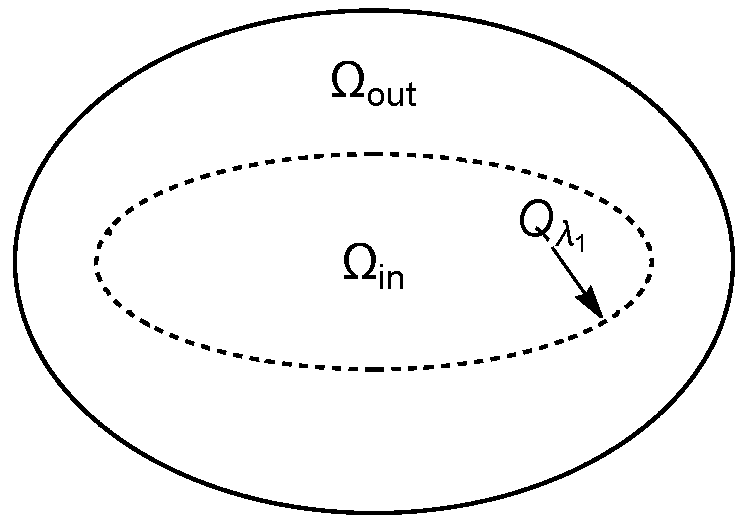
\includegraphics[scale=0.4]{images/section2/domain_problemA.pdf}
    \caption{Область $\Omega$ для задачи А.}
    \label{fig:pt9:_problemA}
\end{figure}

В области $\Omega = \Omega_{in} \cup \Omega_{out}$ рассмотрим бильярдную систему, подчиняющуюся закону $(\ast)$. В работе \cite{vestnikLatest} показано, что для любой бильярдной траектории ее отрезки, лежащие в области $\Omega_{in}$, касаются одной и той же  софокусной квадрики с параметром $\alpha_{in} \in (\lambda_1, a^2)$, а ее отрезки, лежащие в $\Omega_{out}$ --- вообще говоря, другой квадрики с параметром $\alpha_{out} \in (0, a^2)$. При этом параметры $\alpha_{in}$ и $\alpha_{out}$ связаны соотношением $(\alpha_{out} - \lambda_1) n_{out}^2 = (\alpha_{in} - \lambda_1) n_{in}^2$.

Введем функцию $\Lambda$ положения и скорости материальной точки по формуле 
$\Lambda(x, y, v_x, v_y) =  \dfrac{a^2 v_y^2 + b^2v_x^2 - (x v_y-y v_x)^2}{v_x^2 + v_y^2}$. 
Она имеет смысл коэффициента $\alpha$  софокусной квадрики $Q_\alpha$, которая касается прямой, проходящей через точку $(x,y)$ в направлении вектора $(v_x, v_y)$.
Для классического бильярда в эллипсе эта величина является первым интегралом, не зависящим от полной энергии.

Введем функцию  $\Xi(x, y, v_x, v_y)$ по формуле: 
\begin{equation*}
\Xi(x, y, v_x, v_y) = \left[
\begin{array}{ll}
    \Lambda(x, y, v_x, v_y) n_{in}^2, &  \text{ если } (x,y) \in \Omega_{in} \\
    \Lambda(x, y, v_x, v_y) n_{out}^2 + \lambda_1 (n_{in}^2-n_{out}^2), & \text{ если } (x,y) \in \Omega_{out}    .
\end{array}
\right.
\end{equation*}
Она принимает одно и то же значение на любых отрезках траекторий, лежащих как в $\Omega_{in}$ так и в $\Omega_{out}$. Этот факт следует из равенства $(\alpha_{out} - \lambda_1) n_{out}^2 = (\alpha_{in} - \lambda_1) n_{in}^2$ (см. \cite{vestnikLatest}). 

Задача состоит в том, чтобы для указанной динамической системы описать слоение изоэнергетического трехмерного многообразия  на поверхности уровня первого интеграла $\Xi$.

Рассмотрим плоскость $\mathbb{R}^2$ и отложим по горизонтальной оси величину $\alpha_{in}$ и $\alpha_{out}$ -- по вертикальной оси.
Значению интеграла $\Xi$ поставим в соответствие точку плоскости по формуле
\begin{equation}
\Xi \mapsto \alpha(\Xi) = (\alpha_{in}, \alpha_{out} ) = \left( \frac{\Xi}{n_{in}^2}, \frac{\Xi - \lambda_1 (n_{in}^2 - n_{out}^2)}{n_{out}^2} \right) = \left( \left. \Lambda \right|_{\Omega_{in}}, \left. \Lambda \right|_{\Omega_{out}} \right).
\label{XiToLine}
\end{equation}

Для фиксированных $\lambda_1, n_{in}, n_{out}$ точка $\alpha(\Xi)$ лежит на прямой $L$, которая в декартовых координатах $(\alpha_{in}, \alpha_{out})$ задается уравнением
\begin{equation}
\alpha_{out} = \alpha_{in} \left(\frac{n_{in}}{n_{out}}\right)^2 + \lambda_1 \frac{n_{out}^2 - n_{in}^2}{n_{out}^2}.
\label{eq:L_line}
\end{equation}
Отметим, что прямая $L$ проходит через точку $(\lambda_1, \lambda_1)$ и имеет угловой коэффициент наклона, равный $\frac{n_{in}^2}{n_{out}^2}$. Наглядно можно представлять себе, что возможные случаи соотношений между числами $\lambda_1, n_{in}, n_{out}$ соответствуют всевозможным прямым, проходящим через точку $(\lambda_1, \lambda_1)$ и образующим угол с горизонтальной осью, который меняется от $0$ до  $\frac{\pi}{2}$.

Мы введем структурную диаграмму критических значений первого интеграла $\Xi$. 
Бильярдные траектории могут иметь один из следующих типов, см. рис. \ref{fig:pt9:_causticTypesBulletsDiagram}.
\begin{figure}[!htb]
\minipage{0.45\textwidth}
\centering
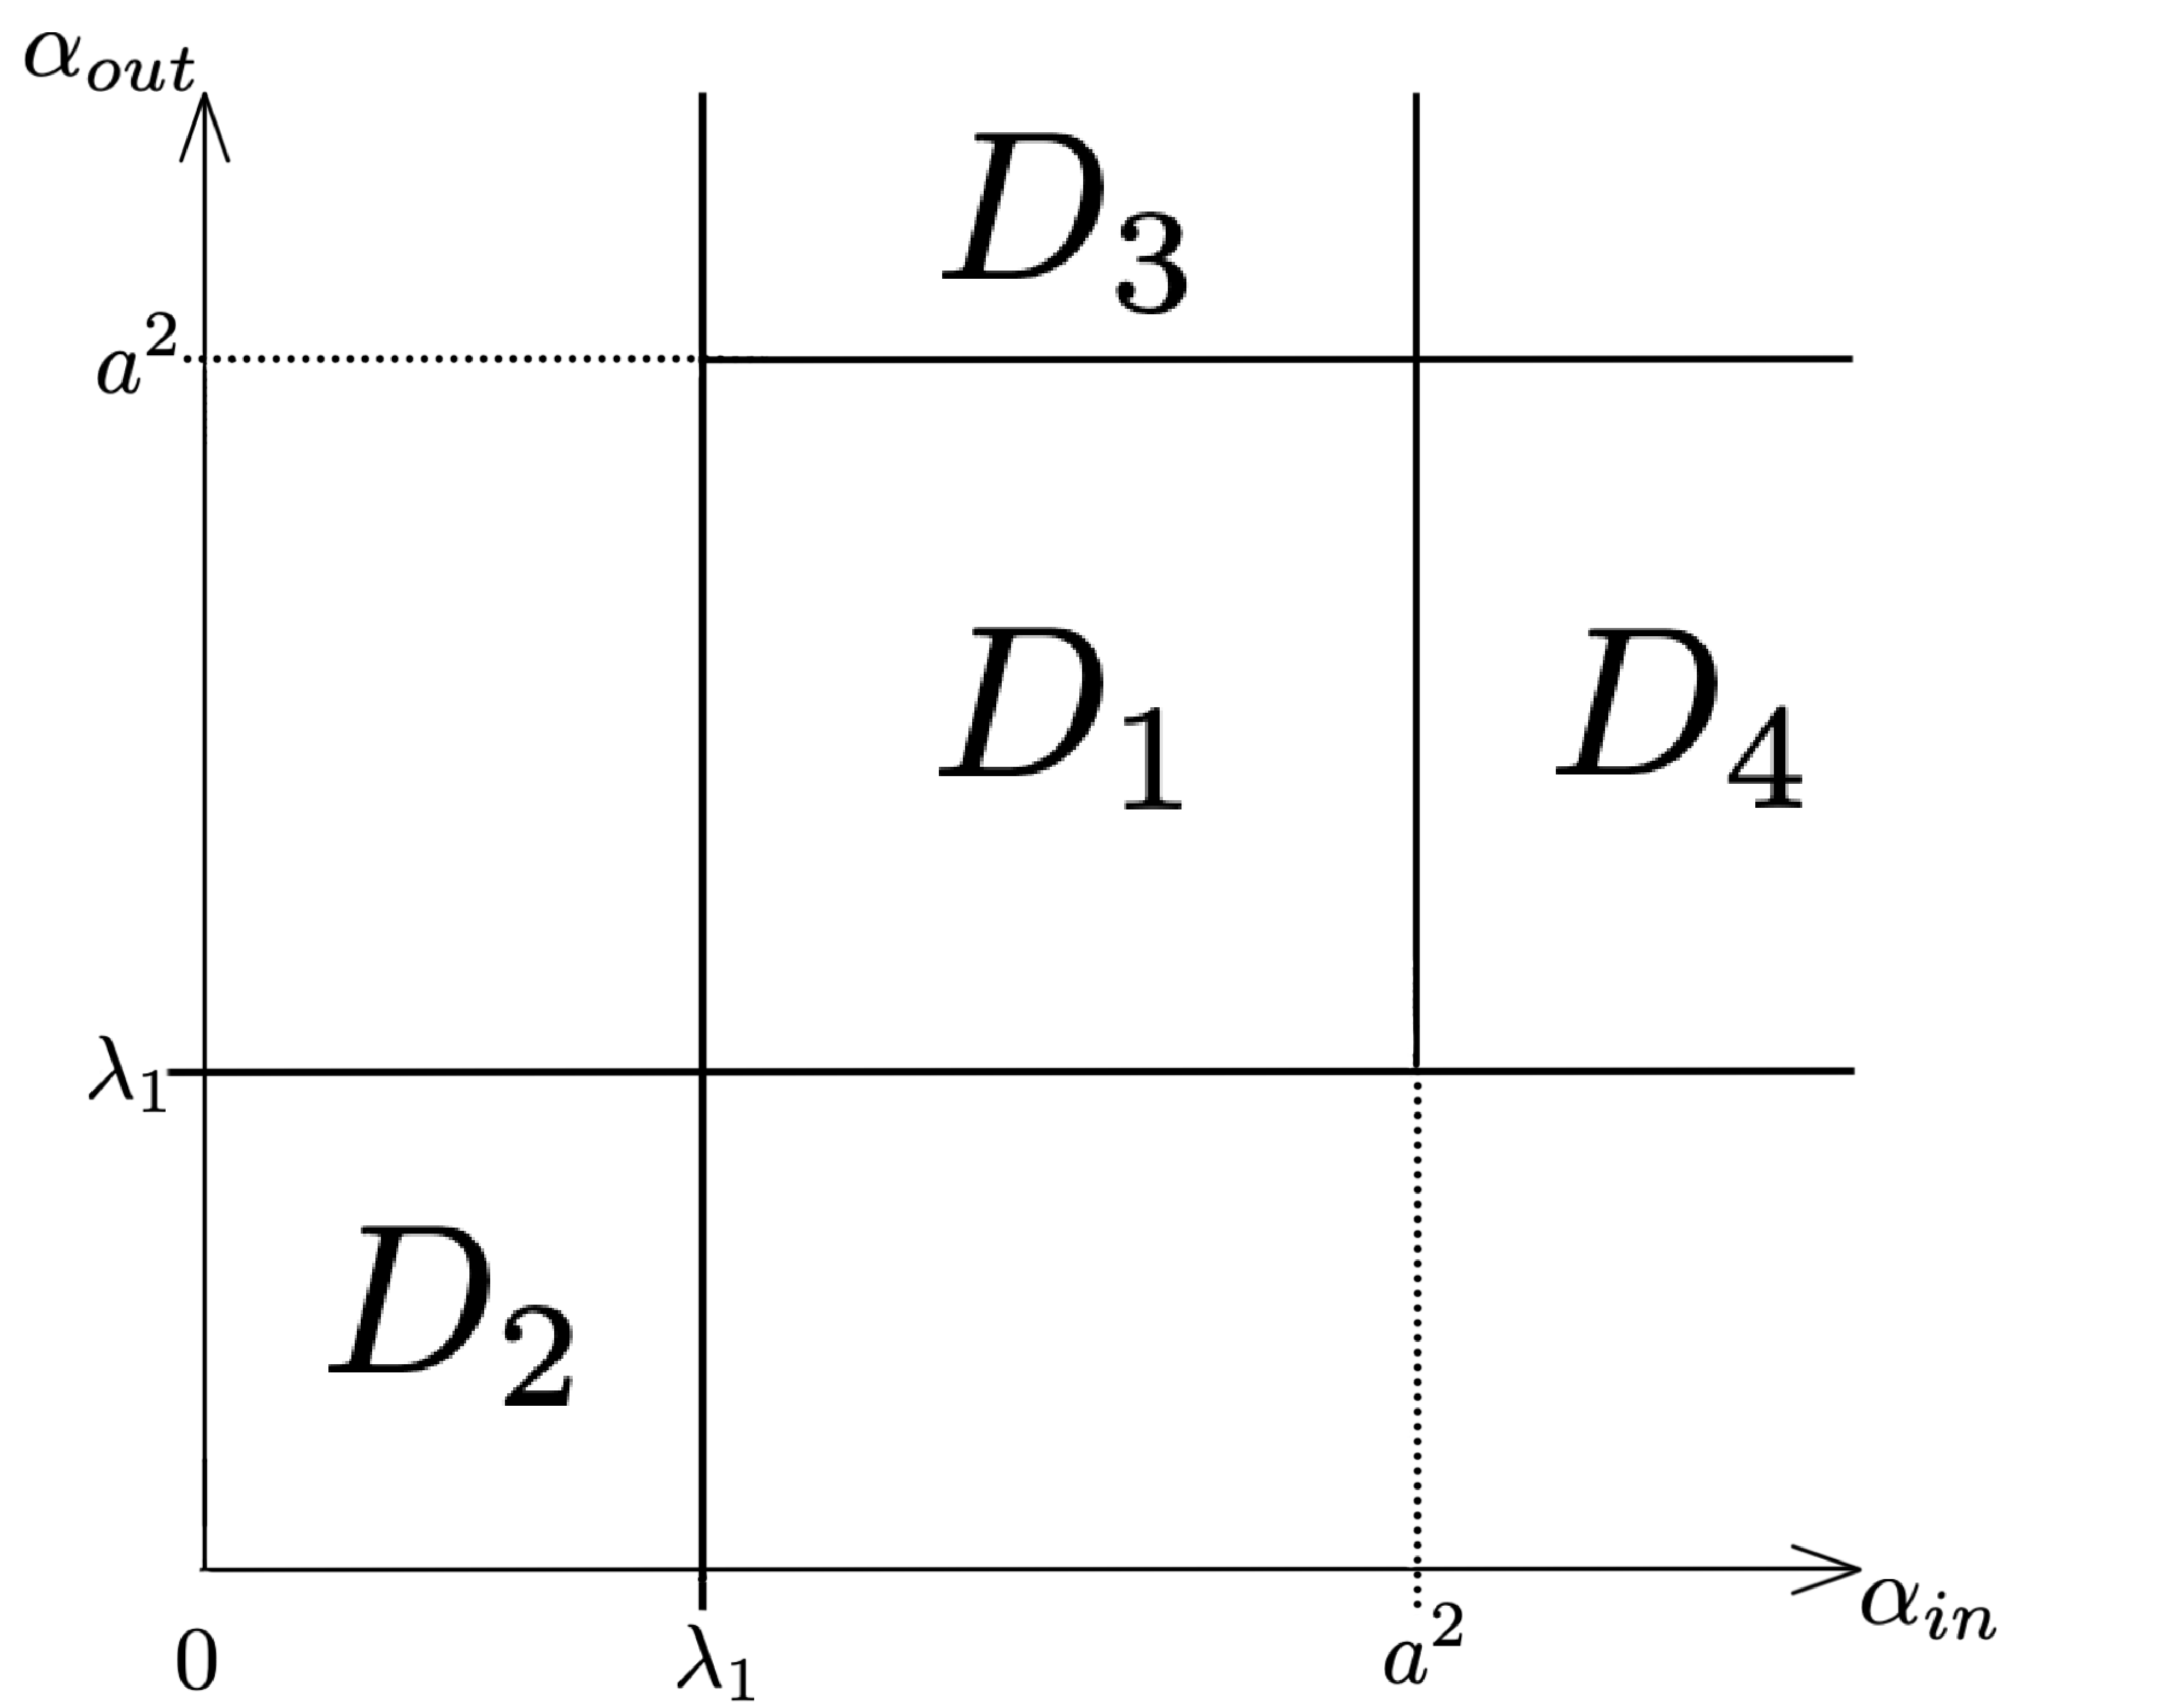
\includegraphics[scale=0.1]{images/section2/causticTypesBulletsDiagram.pdf}
    \caption{Области возможного движения бильярдной траектории.}
    \label{fig:pt9:_causticTypesBulletsDiagram}
\endminipage\hfill
\minipage{0.55\textwidth}
\centering
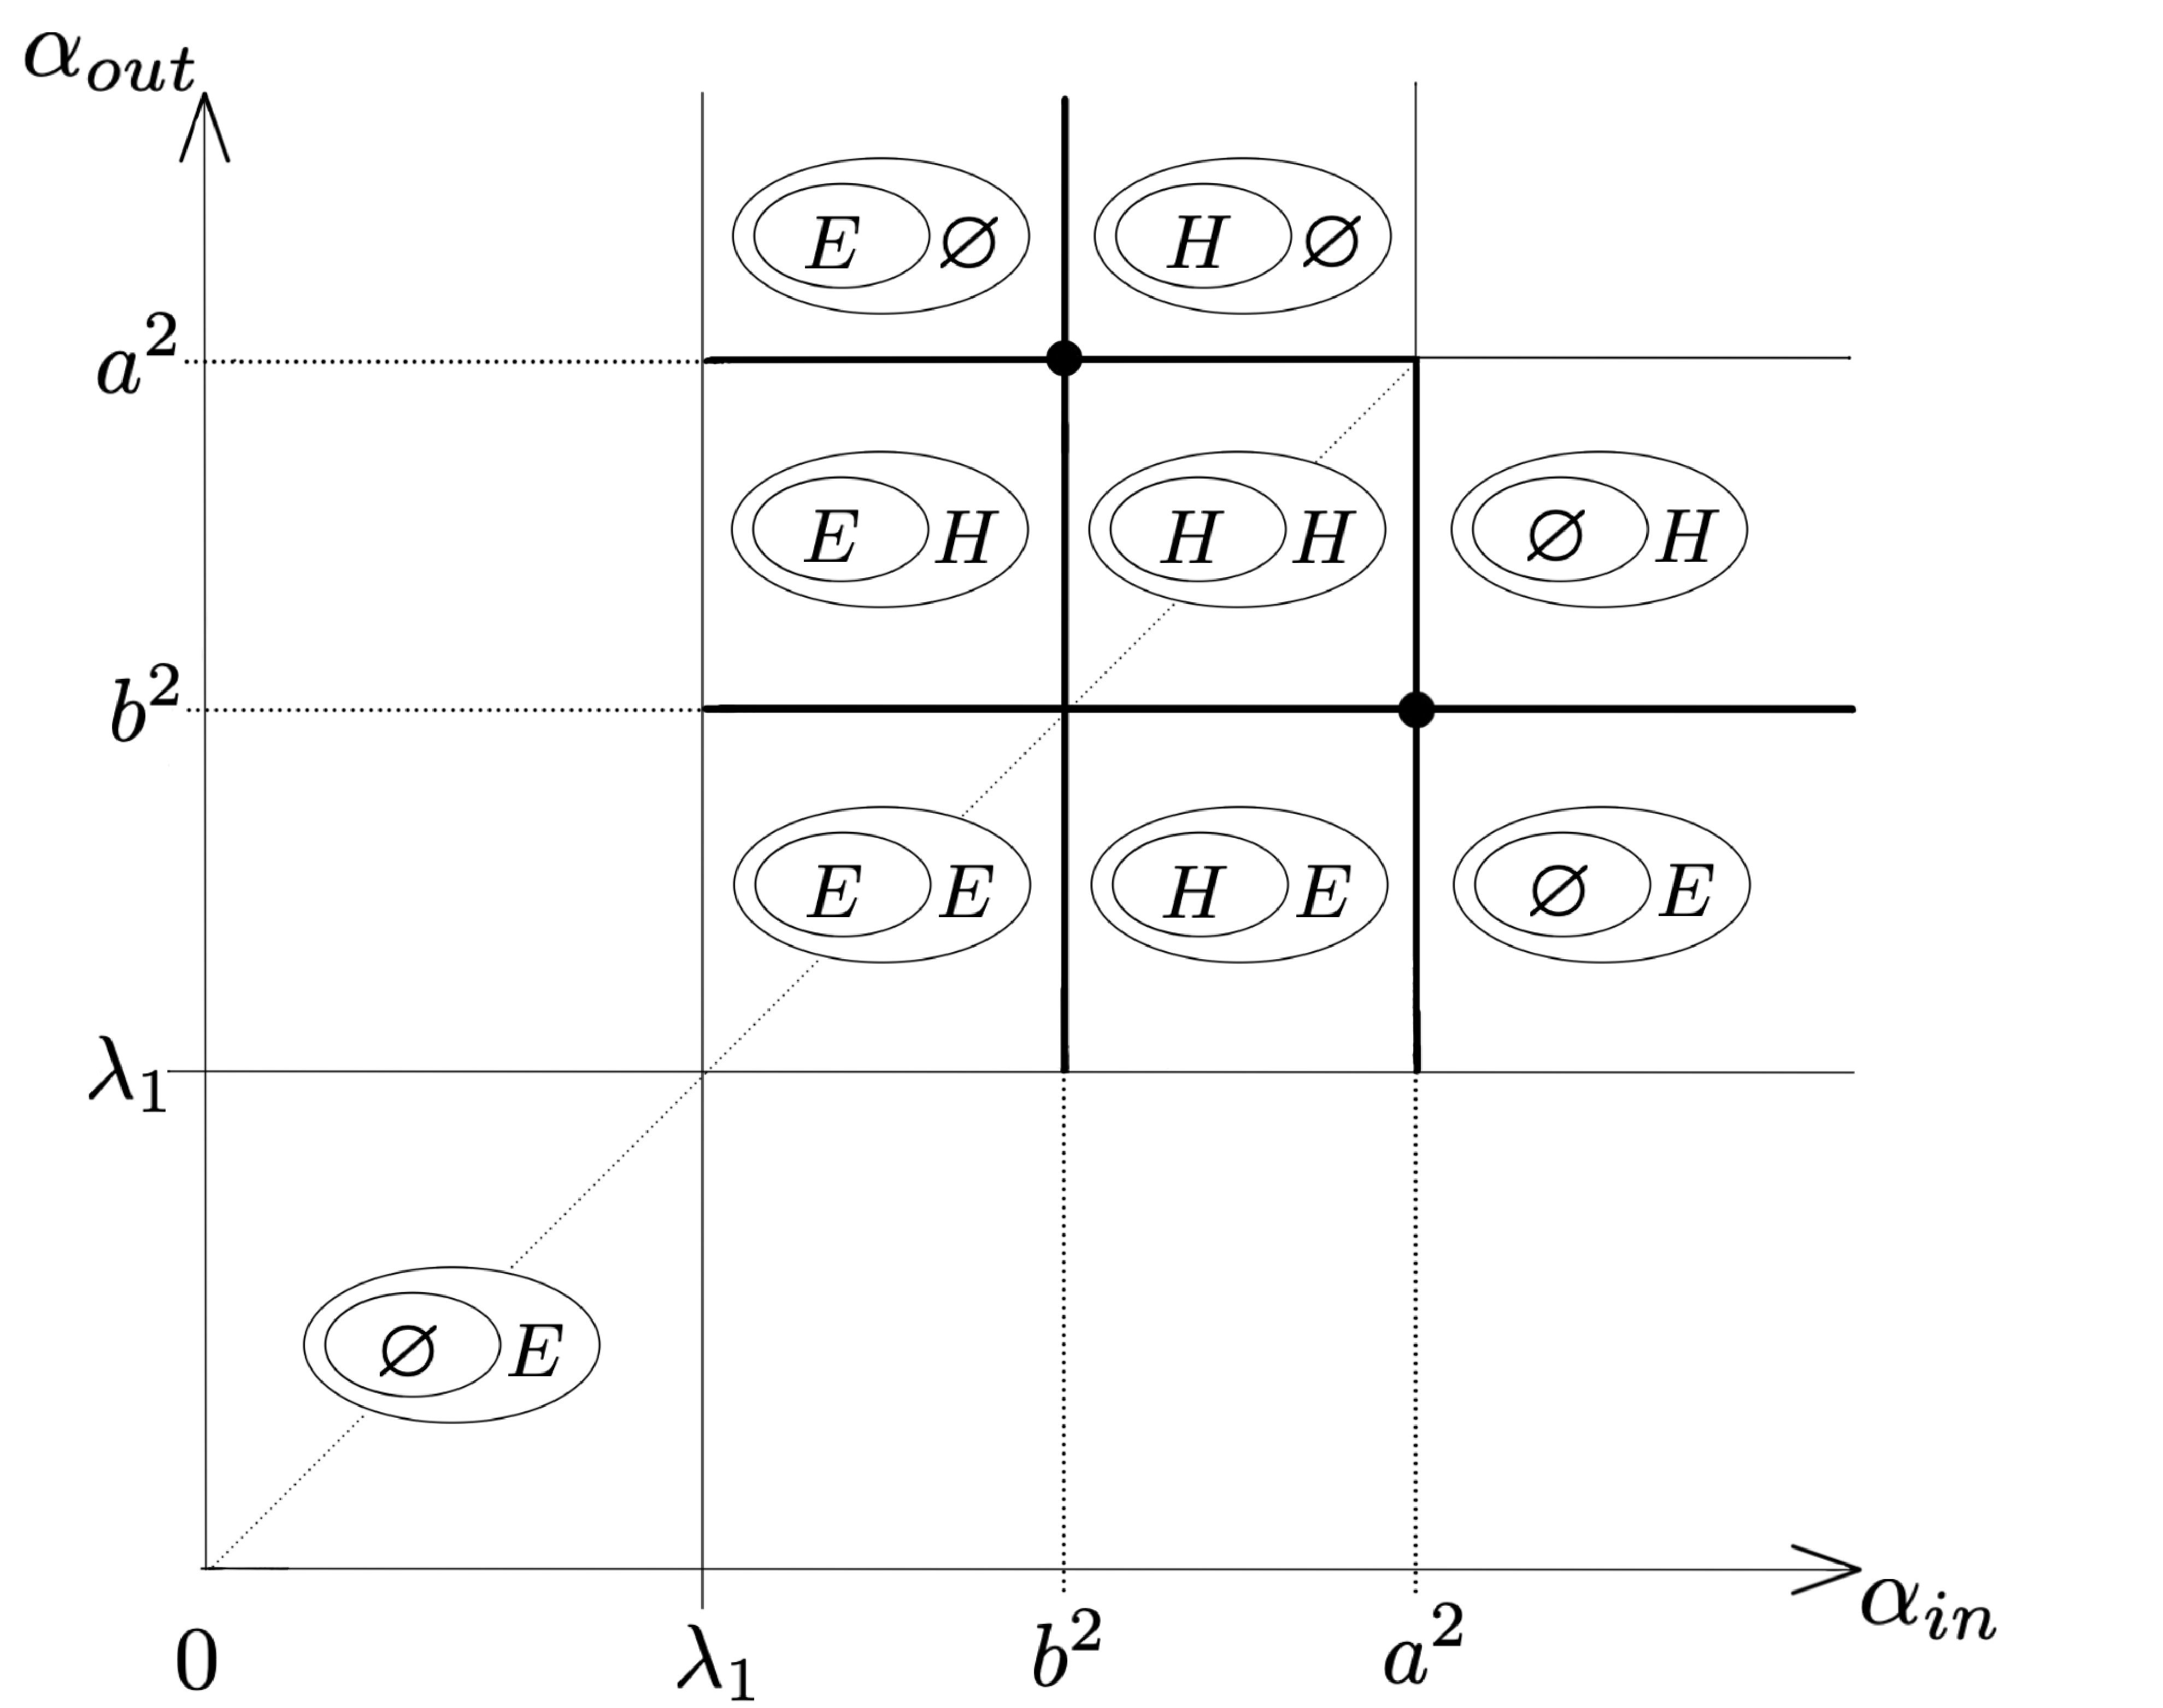
\includegraphics[scale=0.1]{images/section2/problemAbifurcations.pdf}
    \caption{Возможные типы каустик в $\Omega_{in}$ и $\Omega_{out}$. Жирным выделены особые значения для $\alpha_{in}$, $\alpha_{out}$. См. также замечание \ref{rem:remark1}.}
    \label{fig:pt9:_problemAbifurcations}
\endminipage\hfill
\end{figure}

$D1:$ Сначала рассмотрим траекторию, которая заходит в каждую из областей $\Omega_{in}$ и $\Omega_{out}$.
Будем обозначать через $\alpha_{in}$ и $\alpha_{out}$ параметры квадрик, которых касаются отрезки траектории бильярда, находящиеся в областях $\Omega_{in}$ и $\Omega_{out}$, соответственно. В этом случае  $\alpha_{in} \in (\lambda_1, a^2)$, $\alpha_{out} \in (0, a^2)$.

$D2:$ Возможна траектория, целиком находящаяся в области $\Omega_{out}$ и имеющая каустикой эллипс. В этом случае параметр $\alpha_{in}$ не определен, а $\alpha_{out}$ лежит в интервале $\alpha_{out} \in (0, \lambda_1)$.

$D3:$ В случае, если траектория целиком содержится в $\Omega_{in}$, параметр $\alpha_{out}$ не определен. При этом если траектория имеет каустикой эллипс, то $\alpha_{in}$ лежит в интервале $(\lambda_1, b^2)$, а если гиперболу --- в интервале $(b^2, a^2)$.
 Такие траектории испытывают полное внутреннее отражение на границе областей $\Omega_{in}, \Omega_{out}$ и возникают при определенных соотношениях между параметрами $n_{in}, n_{out}$. 

$D4:$ Для траекторий, целиком находящихся в области $\Omega_{out}$ и имеющих каустикой гиперболу,  параметр $\alpha_{in}$ также не определен, а $\alpha_{out}$ лежит в интервале $(b^2, a^2)$.
Такие траектории также испытывают полное внутреннее отражение на границе областей $\Omega_{in}, \Omega_{out}$ и возникают при определенных соотношениях между параметрами $n_{in}, n_{out}$.


Анализ слоения на поверхности уровня интеграла $\Xi$ проходит по следующей схеме.
Сначала фиксируются параметры $\lambda_1, n_{in}, n_{out}$. Они определяют прямую $L$, при этом значение интеграла $\Xi$ однозначно определяет точку на этой прямой. Структура слоения определяется тем, как прямая $L$ пересекает области $D_1, D_2, D_3, D_4$.
Пересечение прямой $L$ с областью $D_1$ определяет значения $\Xi$, при которых имеет место движение типа $D_1$; определены оба параметра $\alpha_{in}, \alpha_{out}$.
Пересечение этой прямой с областью $D_2$ определяет движение типа $D_2$, и при этом  параметр $\alpha_{in}$ не имеет смысла; для $D_3$ аналогично. 
Пересечение прямой с областью $D_4$ определяет движение типа $D_4$, в этом случае не  определен параметр $\alpha_{out}$.

%Это соотношение имеет смысл рассматривать для случая $D_1$. Для случаев $D_2$ и $D_3$ параметр $\alpha_{in}$ не определен. Для случая $D_4$ не определен параметр $\alpha_{out}$. Для фиксированных значений $n_{in}, n_{out}, \lambda_1$ соответствие $\Xi \mapsto \alpha(\Xi)$
%\begin{remark} 
%Заметим, что при $0 < \alpha_{out} < \lambda_1$ траектория бильярда целиком находится в $\Omega_{out}$ и не попадает в область $\Omega_{in}$. 
%Следовательно, параметр $\alpha_{in}$ в этом случае не определен.
%Поэтому принадлежность интеграла $\Xi$ этой прямой в квадрате $0 < \alpha_{in}, \alpha_{out} < \lambda_1$ и в областях $\alpha_{in}, \alpha_{out} > a^2$ весьма условная. Мы не будем заострять на этом внимание в угоду наглядности диаграммы \ref{fig:pt9:_causticTypesDiagram}.
%\end{remark}

%(0, \lambda_1 \left(1 - \frac{n_{in}^2}{n_{out}^2}\right) )$. Интеграл $\Xi$ соответствует некоторой точке на этой прямой. 


При этом нерегулярные значения интеграла $\Xi$ соответствуют точкам пересечения  прямой $L$ с координатными линиями $\alpha_{in},\alpha_{out} = b^2, a^2$, изображенным жирными линиями на рис. \ref{fig:pt9:_problemAbifurcations}.
Особый интерес вызывают случаи, когда $L$ проходит через точку $(\alpha_{in}, \alpha_{out}) = (a^2, b^2)$ или точку  $(\alpha_{in}, \alpha_{out}) = (b^2, a^2)$.
\begin{remark}
В случае, когда совпадают коэффициенты $n_{in}$ и $n_{out}$, траектории проходят из $\Omega_{in}$ в $\Omega_{out}$ и обратно без преломления, тем самым мы получаем динамику классического бильярда в эллипсе. Этому соответствует прямая $L$, проходящая по пунктирной диагонали на рис. \ref{fig:pt9:_problemAbifurcations}.

На рис. \ref{fig:pt9:_problemAbifurcations} схематично показаны типы каустик в областях $\Omega_{in}$ и $\Omega_{out}$:  $H$ означает, что каустика является гиперболой, $E$ соответствует эллипсу, а $\varnothing$ означает, что траектория не заходит внутрь соответствующей области. 
\label{rem:remark1}
\end{remark}
%Для удобства занумеруем регулярные области значений интеграла $\Xi$ на рис. \ref{fig:pt9:_causticTypesDiagram}.
%В ходе их описания мы узнаем как выглядят соответствующие области $\Omega$. Потом, когда будем описывать бифуркации, 

Параметры  $\alpha_{in}$, $\alpha_{out}$ имеют критические значения $b^2, a^2$. Соответствующие вертикальные и горизонтальные прямые, а также диагональ $\alpha_{in} = \alpha_{out}$, разбивают области $D_1, \ldots, D_4$ на подобласти, показанные на рис. \ref{fig:pt9:_problemA_subdivisions}. Формально эти подобласти определены в теореме \ref{st:pt9:n1_n2_surfaces}.
\begin{figure}[!htb]
\centering
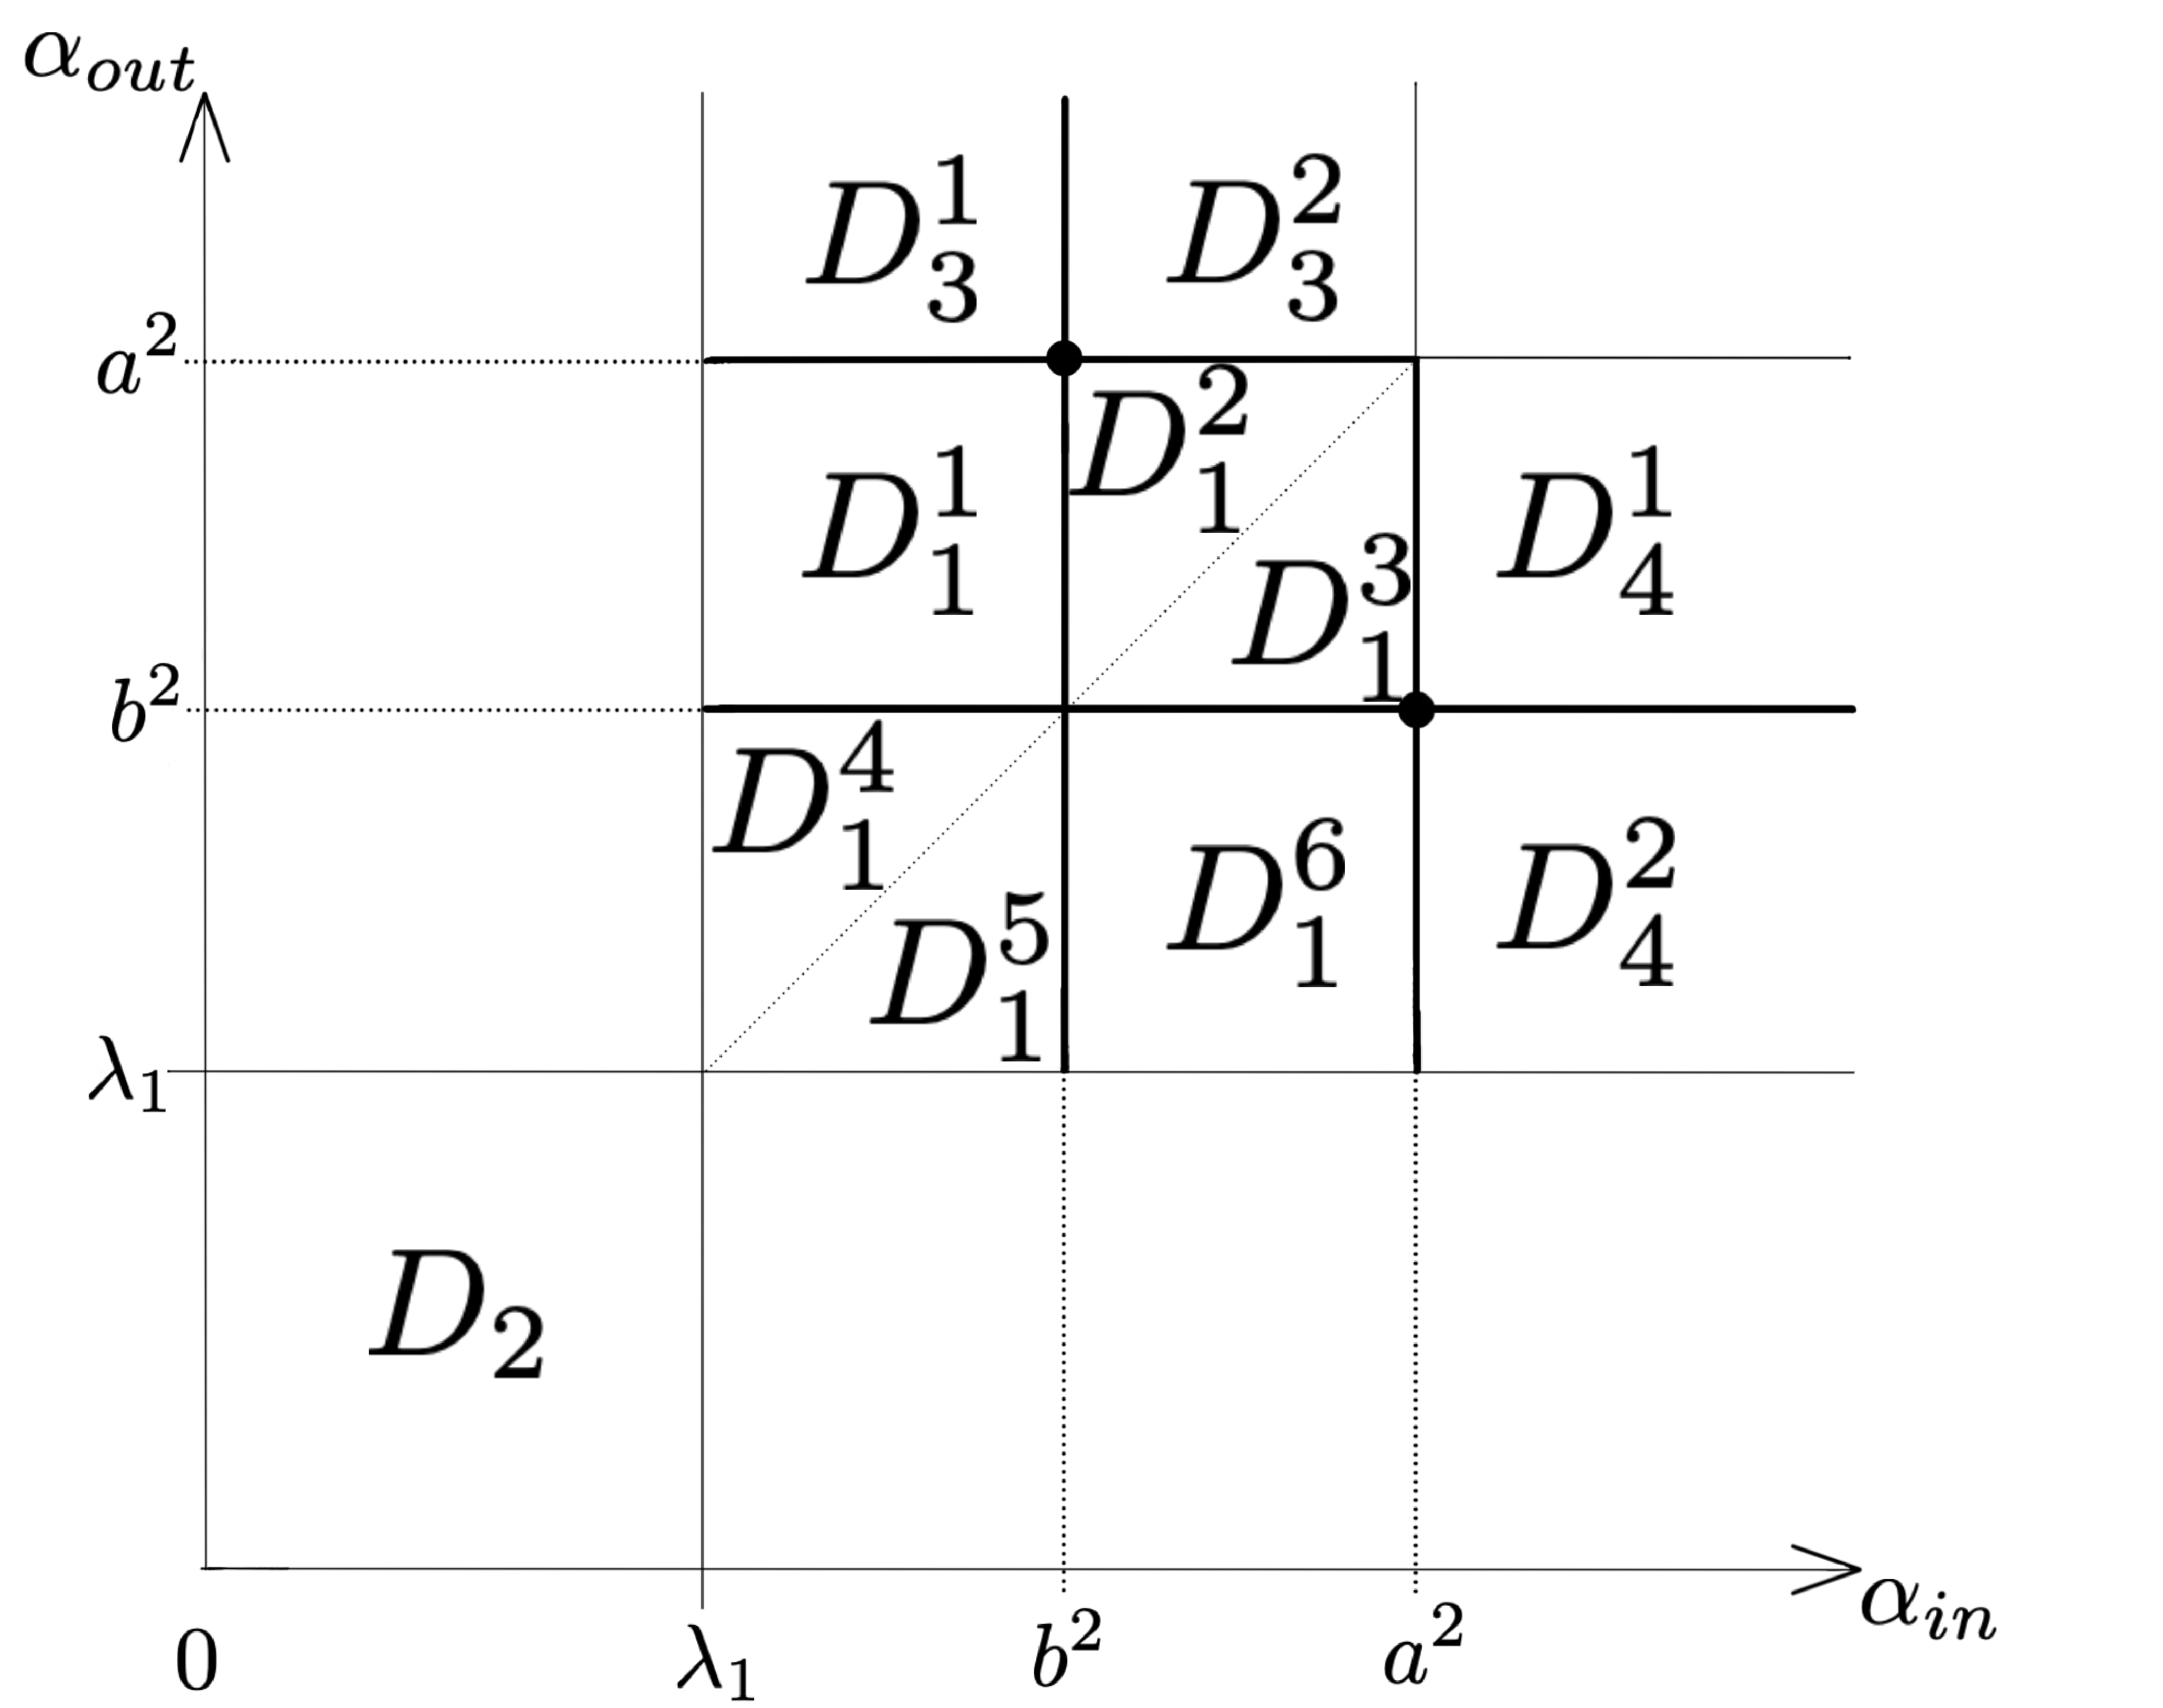
\includegraphics[scale=0.1]{images/section2/problemA_subdivisions.pdf}
    \caption{Подразбиение областей $D_1, \ldots, D_4$.}
    \label{fig:pt9:_problemA_subdivisions}
\end{figure}

\subsection{Поверхности уровня для регулярных значений интеграла $\Xi$}
\begin{theorem} 
Областям $D_i^j$ в плоскости $(\alpha_{in}, \alpha_{out})$ соответствуют следующие поверхности $\Xi = \const$
\medskip
\begin{center}
\begin{tabular}{|c|c|c|}
\hline 
$D_1^1$  	& 	$\alpha_{in} \in (\lambda_1, b^2), \ \alpha_{out} \in (b^2, a^2)$			& сфера с 5 ручками; \\ \hline 
$D_1^2$  	& 	$\alpha_{in} \in (b^2, a^2), \ \alpha_{out} \in (\alpha_{in}, a^2)$				& сфера с 5 ручками; \\ \hline 
$D_1^3$  	& 	$\alpha_{in} \in (b^2, a^2), \ \alpha_{out} \in (b^2, \alpha_{in})$				& сфера с 5 ручками; \\ \hline 
$D_1^4$ 	& 	$\alpha_{in} \in (\lambda_1, b^2), \ \alpha_{out} \in (\alpha_{in}, b^2)$	& 2 дизъюнктных тора; \\ \hline 
$D_1^5$  	& 	$\alpha_{in} \in (\lambda_1, b^2), \ \alpha_{out} \in (\lambda_1, \alpha_{in})$	& 2 дизъюнктных тора; \\ \hline 
$D_1^6$  	& 	$\alpha_{in} \in (b^2, a^2), \ \alpha_{out} \in (\lambda_1, b^2)$			& сфера с 5 ручками; \\ \hline 
\hline
$D_2$  	& 	$(\alpha_{out} \in (0, \lambda_1), \ \alpha_{in} < \lambda_1)$ или & \\
		&  $(\alpha_{in} \in (0, \lambda_1), \ \alpha_{out} < \lambda_1)$				& 2 дизъюнктных тора; \\ \hline
 \hline
$D_3^1$  	& 	$\alpha_{in} \in (\lambda_1, b^2), \ \alpha_{out} > a^2$				& 2 дизъюнктных тора; \\ \hline 
$D_3^2$  	& 	$\alpha_{in} \in (b^2, a^2), \ \alpha_{out} > a^2 $					& 1 тор; \\ \hline 
\hline 
$D_4^1$  	& 	$\alpha_{in} > a^2, \ \alpha_{out} \in (b^2, a^2)$						& 2 дизъюнктных тора; \\ \hline 
$D_4^2$  	& 	$\alpha_{in} > a^2, \alpha_{out} \in (\lambda_1, b^2)$				& 2 дизъюнктных тора; \\ \hline 
\end{tabular}
\end{center}
%\[
%\begin{array}{c|c|c}
%D_2  & & \text{2 дизъюнктных тора}; \\
%
%
%\alpha_{out} \in (\lambda_1, b^2) & \alpha_{in} \in (\lambda_1, b^2) &  \text{2 дизъюнктных тора}; \\
% & \alpha_{in} \in (b^2, a^2) &  \text{сфера с 5 ручками}; \\
% & \alpha_{in} > a^2 &   \text{2 дизъюнктных тора}; \\
%
%\alpha_{out} \in (b^2, a^2)  & \alpha_{in} \in (\lambda_1, b^2) &  \text{сфера с 5 ручками}; \\
% & \alpha_{in} \in (b^2, a^2), \ \alpha_{in} \neq \alpha_{out} &  \text{сфера с 5 ручками}; \\
%  & \alpha_{in} \in (b^2, a^2), \ \alpha_{in} = \alpha_{out} &  \text{тор}; \\
% & \alpha_{in}  > a^2 &   \text{2 дизъюнктных тора}; \\
%
%\alpha_{out} > a^2 & \alpha_{in} \in (\lambda_1, b^2) &  \text{2 дизъюнктных тора}; \\
% & \alpha_{in} \in (b^2, a^2) &  \text{1 тор}. \\
%\end{array}
%\]
\label{st:pt9:n1_n2_surfaces}
\end{theorem} 



\begin{proof}

%Доказательство будет основываться на соображениях, предложенных в \cite[\S 3]{Fok15}.

\textbf{Случай $D_1^4$, $D_1^5$.}
%Касательные к траекториям бильярда в области $\Omega_{out}$ будут касаться некоторого эллипса с параметром $\alpha_{out}$. В области $\Omega_{in}$ параметром такого эллипса выступает $\alpha_{in}$. 
Продолжения звеньев траектории, лежащих в $\Omega_{out}$, касаются каустики с параметром $\alpha_{out}$, а звенья траектории в области $\Omega_{in}$ касаются каустики с параметром $\alpha_{in}$. При этом оба параметра $\alpha_{in}, \alpha_{out}$ находятся в интервале $(\lambda_1, b^2)$, то есть обе каустики являются эллипсами.

Спроектируем точку траектории $(x,y,v_x, v_y)$ на бильярдную область:
$$\pi : (x,y,v_x, v_y) \mapsto (x, y).$$
Рассмотрим всевозможные траектории с фиксированным значением $\Xi$, относящимся к случаям $D_1^4, D_1^5$. Тогда проекция $(x,y) \in \Omega_{out}$ заметает всю область $\Omega_{out}$, а проекция  $(x,y) \in \Omega_{in}$ заметает кольцо $\widetilde{\Omega}_{in} = \Omega_{in} \setminus \text{ int }(\Omega_{\alpha_{in}})$, где $\Omega_{\alpha_{in}}$ --- это область, ограниченная квадрикой $Q_{\alpha_{in}}$. 

Поверхность $\Xi = \const$ склеена из нескольких копий $\widetilde{\Omega}_{in}$ и $\Omega_{out}$. 

Во всех внутренних точках $\widetilde{\Omega}_{in}$ и $\Omega_{out}$ проекция $(x, y, v_x, v_y) \mapsto (x,y)$ четырехлистная.
В прообразе этой проекции на поверхности $\Xi = \const$ выберем по 4 прообраза для областей $\Omega_{out}$ и $\widetilde{\Omega}_{in}$, обозначим эти прообразы 
$\Omega_{out, j}$ и $\Omega_{in, j}$, $j=1,\ldots,4$, 
где нумерация определена по следующему правилу:

\begin{equation}
\begin{array}{ll}
1: & \text{ вектор } (v_x, v_y) \text{ направлен по часовой стрелке к эллипсу } Q_{\alpha}, \\
2: & \text{ вектор } (v_x, v_y) \text{ направлен против часовой стрелки к эллипсу }  Q_{\alpha}, \\
3: & \text{ вектор } (v_x, v_y) \text{ направлен против часовой стрелки от эллипса }  Q_{\alpha}, \\
4: & \text{ вектор } (v_x, v_y) \text{ направлен по часовой стрелке от эллипса }  Q_{\alpha},
\end{array}
\label{eq:ell_numeration}
\end{equation}
где $\alpha$ --- параметр каустики, т.е. $\alpha=\alpha_{out}$ для $(x,y) \in \Omega_{out}$ и $\alpha=\alpha_{in}$ для $(x,y) \in \widetilde{\Omega}_{in}$.

Поверхность $\Xi=\const$ в рассматриваемом случае склеена из 8 эллиптических колец $\Omega_{out, j}, \Omega_{in, j}, \ j=1, \ldots, 4$. 
Проследим правила склейки:

$\bullet$ $\Omega_{out, j}$ и $\Omega_{in, j}$ отождествляются по общей границе, которая проектируется в $Q_{\lambda_1}$, поскольку правила $(\ast)$ сохраняют номер в случае, когда обе каустики являются эллипсами.
Получим 4 области, которые обозначим как $\widetilde{\Omega}_1, \widetilde{\Omega}_2, \widetilde{\Omega}_3, \widetilde{\Omega}_4$, где $\widetilde{\Omega}_j = \Omega_{out, j} \cup \widetilde{\Omega}_{in, j}, \ j=1, \ldots, 4$.

$\bullet$ На внешней границе $\widetilde{\Omega}_1$ приклеивается к $\widetilde{\Omega}_4$, а $\widetilde{\Omega}_2$ к $\widetilde{\Omega}_3$ в силу стандартного закона отражения.

$\bullet$ На внутренней границе $\widetilde{\Omega}_1$ подклеивается к $\widetilde{\Omega}_4$, а $\widetilde{\Omega}_2$ подклеивается к $\widetilde{\Omega}_3$ в силу смены номера листа после касания звеном траектории каустики $Q_{\alpha_{in}}$.

%\textcolor{red}{старое}
%Рассмотрим область, которая целиком содержит траекторию бильярда, то есть область 
%$\widetilde{\Omega} = \Omega_{out} \cup \widetilde{\Omega}_{in} = \Omega_{out} \cup (\Omega_{in} \setminus \text{ int } Q_{\alpha_{in}})$, 
%где из $\Omega_{in}$ мы вырезаем внутренность эллипса с параметром $\alpha_{in}$. 
%
%В произвольной внутренней точке $\widetilde{\Omega}$, исключая $Q_{\lambda_1}$,  определены 4 вектора скорости $(v_x, v_y)$ таких, что $(x, y, v_x, v_y)$ лежит на соответствующем уровне интеграла $\Xi$. 
%А именно, векторы принадлежат касательной к каустике $Q_{\alpha_{in}}$ для $(x, y) \in \Omega_{in}$ или к каустике $Q_{\alpha_{out}}$ для $(x, y) \in \Omega_{out}$.
%
%Здесь и далее считаем, что точкам $(x, y) \in \Omega_{in}$ соответствуют векторы $v_i, i=1,\ldots,4$, а точкам $(x, y) \in \Omega_{out}$ --- векторы $w_i, i=1,\ldots,4$.
%Нумерацию векторов для эллиптической каустики установим следующую (см. рис. \ref{fig:pt9:_caseD14}):
%
%\begin{figure}[!htb]
%\centering
%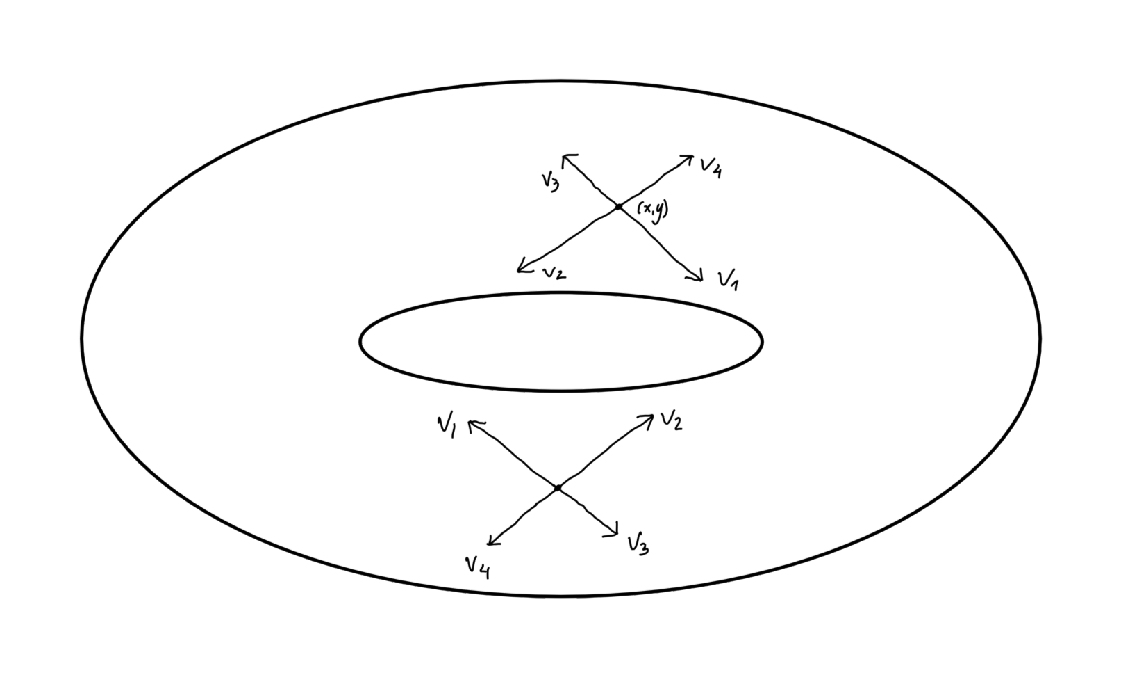
\includegraphics[scale=0.45]{images/section2/caseD14.pdf}
%    \caption{Определение векторов скорости в случае эллиптической каустики.}
%    \label{fig:pt9:_caseD14}
%\end{figure}
%
%\begin{remark}
%Пусть $\alpha$ --- параметр эллиптической каустики, точка $(x,y)$ находится вне эллипса $Q_{\alpha}$, а векторы $\nu_i$ задают касательную к нему, проходящую через $(x,y)$. Тогда нумерацию определим следующим образом:
%\begin{equation}
%\begin{array}{ll}
%\nu_1, & \text{ --  направлен по часовой стрелке к эллипсу } Q_{\alpha}, \\
%\nu_2, & \text{ --  направлен против часовой стрелки к эллипсу }  Q_{\alpha}, \\
%\nu_3, & \text{ --  направлен против часовой стрелки от эллипса }  Q_{\alpha}, \\
%\nu_4, & \text{ --  направлен по часовой стрелке от эллипса }  Q_{\alpha}.
%\end{array}
%\end{equation}
%\label{eq:vectors_roles}
%\end{remark}
%
%Так определим векторы $v_i, \ i=1, \ldots, 4$ для точек $(x,y) \in \widetilde{\Omega}_{in}$.
%Векторы $w_i, \ i=1,\ldots, 4$ для точек $(x,y) \in \widetilde{\Omega}_{out}$ определяются аналогично с точностью до замены эллипса $Q_{\alpha_{in}}$ на $Q_{\alpha_{out}}$.
%
%При этом точки $(x, y) \in Q_{\lambda_1}$ являются граничными для $\Omega_{out}$ и $\Omega_{in}$.
%В этих точках соответствие между векторами $v_i$ и $w_j$ устанавливается исходя из закона преломления $(\ast)$. 
%
%
%Под листом $\Sigma_{i, out}$ будем понимать пару $(\Omega_{out}, w_i)$. Аналогично 
%лист $\Sigma_{j, in}$ обозначает пару $(\widetilde{\Omega}_{in}, v_j)$. 
%%Листы будем подклеивать друг к другу 
%В разбираемом случае на эллипсе с параметром $\lambda_1$ закон преломления влечет \textit{правило склейки} $\Sigma_{i, out} \sim \Sigma_{i, in}$. 
%Для краткости  можем определить большой лист $\Sigma_k$, соответствующий склейке $\Sigma_{k, out} \cup \Sigma_{k, in}$.
%%Здесь и далее это правило склейки $\Omega_{out}$ с $\widetilde{\Omega}_{in}$ используем без явного упоминания соответствия.
%%Очевидно, что такое соответствие локально является непрерывным. 
%
%На дугах внешнего граничного эллипса $Q_0$ закон отражения приводит к слейкам областей $\Sigma_1 \sim \Sigma_4$ и $\Sigma_2 \sim \Sigma_3$. 
%При интегральном эллипсе $Q_{\alpha_{in}}$ в силу тождественного совпадения $v_1 = v_4$ и $v_2 = v_3$ возникают склейки $\Sigma_1 \sim \Sigma_4$ и $\Sigma_2 \sim \Sigma_3$.
Таким образом, для случая  $D_1^4$, $D_1^5$ поверхности уровня интеграла $\Xi$ являются  несвязным объединением двух торов.

%\marginpar{мы устали}
\medskip
\textbf{Случай $D_2$.} 
Траектория целиком содержится в $\Omega_{out}$. Точки проекции $(x,y)$ заметают $\widetilde{\Omega} = \Omega_{out} \setminus \Omega_{\alpha_{out}}$, при этом проекция четырехлистная, как и в предыдущем случае. 
Четыре прообраза $\widetilde{\Omega}$ нумеруются по правилам, указанным в предыдущем случае. 
Внешние и внутренние границы $\widetilde{\Omega}_1$ подклеиваются к соответствующим границам $\widetilde{\Omega}_4$, аналогично для $\widetilde{\Omega}_2$ и $\widetilde{\Omega}_3$. Результатом склейки являются два дизъюнктных тора.
%Повторяя соображения предыдущего случая, на граничном и интегральном торах возникают склейки $\Sigma_1 \sim \Sigma_4$ и $\Sigma_2 \sim \Sigma_3$. Результатом склейки также выступают два тора.

\medskip
\textbf{Случай $D_4^2$. } Траектория снова целиком содержится в $\Omega_{out}$ и отражается от обеих границ внешнего кольца. Рассуждения, аналогичные случаю $D_2$ с той лишь разницей, что вместо $\alpha_{out}$ пишется $\lambda_1$, а вместо касания на внутренней границе используется отражение, показывают, что в этом случае поверхностью уровня $\Xi=\const$ являются два дизъюнктных тора.

\medskip
\textbf{Случай $D_3^1$. } аналогичен случаю $D_4^2$ с той лишь разницей, что траектория целиком содержится в $\Omega_{in}$. Более точно, в кольце между эллипсами $Q_{\lambda_1}$ и $Q_{\alpha_{in}}$. Поверхностью уровня снова служат два тора.

%Остаются еще 2 случая, в которых одна из каустик является эллипсом. При этом вторая будет гиперболой.
%Рассмотрение гиперболических каустик начнем со случая $D_3^2$.

\medskip
\textbf{Случай $D_3^2$.}
Траектория целиком содержится в $\Omega_{in}$, при этом касается ветвей гиперболы с параметром $\alpha_{in}$ и отражается от внешней границы эллипса $\Omega_{in}$.

По аналогии с предыдущими случаями определим $\widetilde{\Omega}$ как часть внутренности области $\Omega_{in}$, лежащую между ветвей гиперболы $Q_{\alpha_{in}}$ (см. рис. \ref{fig:pt9:_hyp_domain_example}). При проекции $\pi$ прообразом области  $\widetilde{\Omega}$ служат 4 листа $\widetilde{\Omega}_{j}, i=1, \ldots, 4$. Нумерацию листов см. рис. \ref{fig:pt9:_hyp_vectors_numbering}. Сплошным изображены те векторы $(v_x, v_y)$ которые направлены в сторону точки касания звена траектории с каустикой.

\begin{figure}[!htb]
\minipage{0.45\textwidth}
\centering
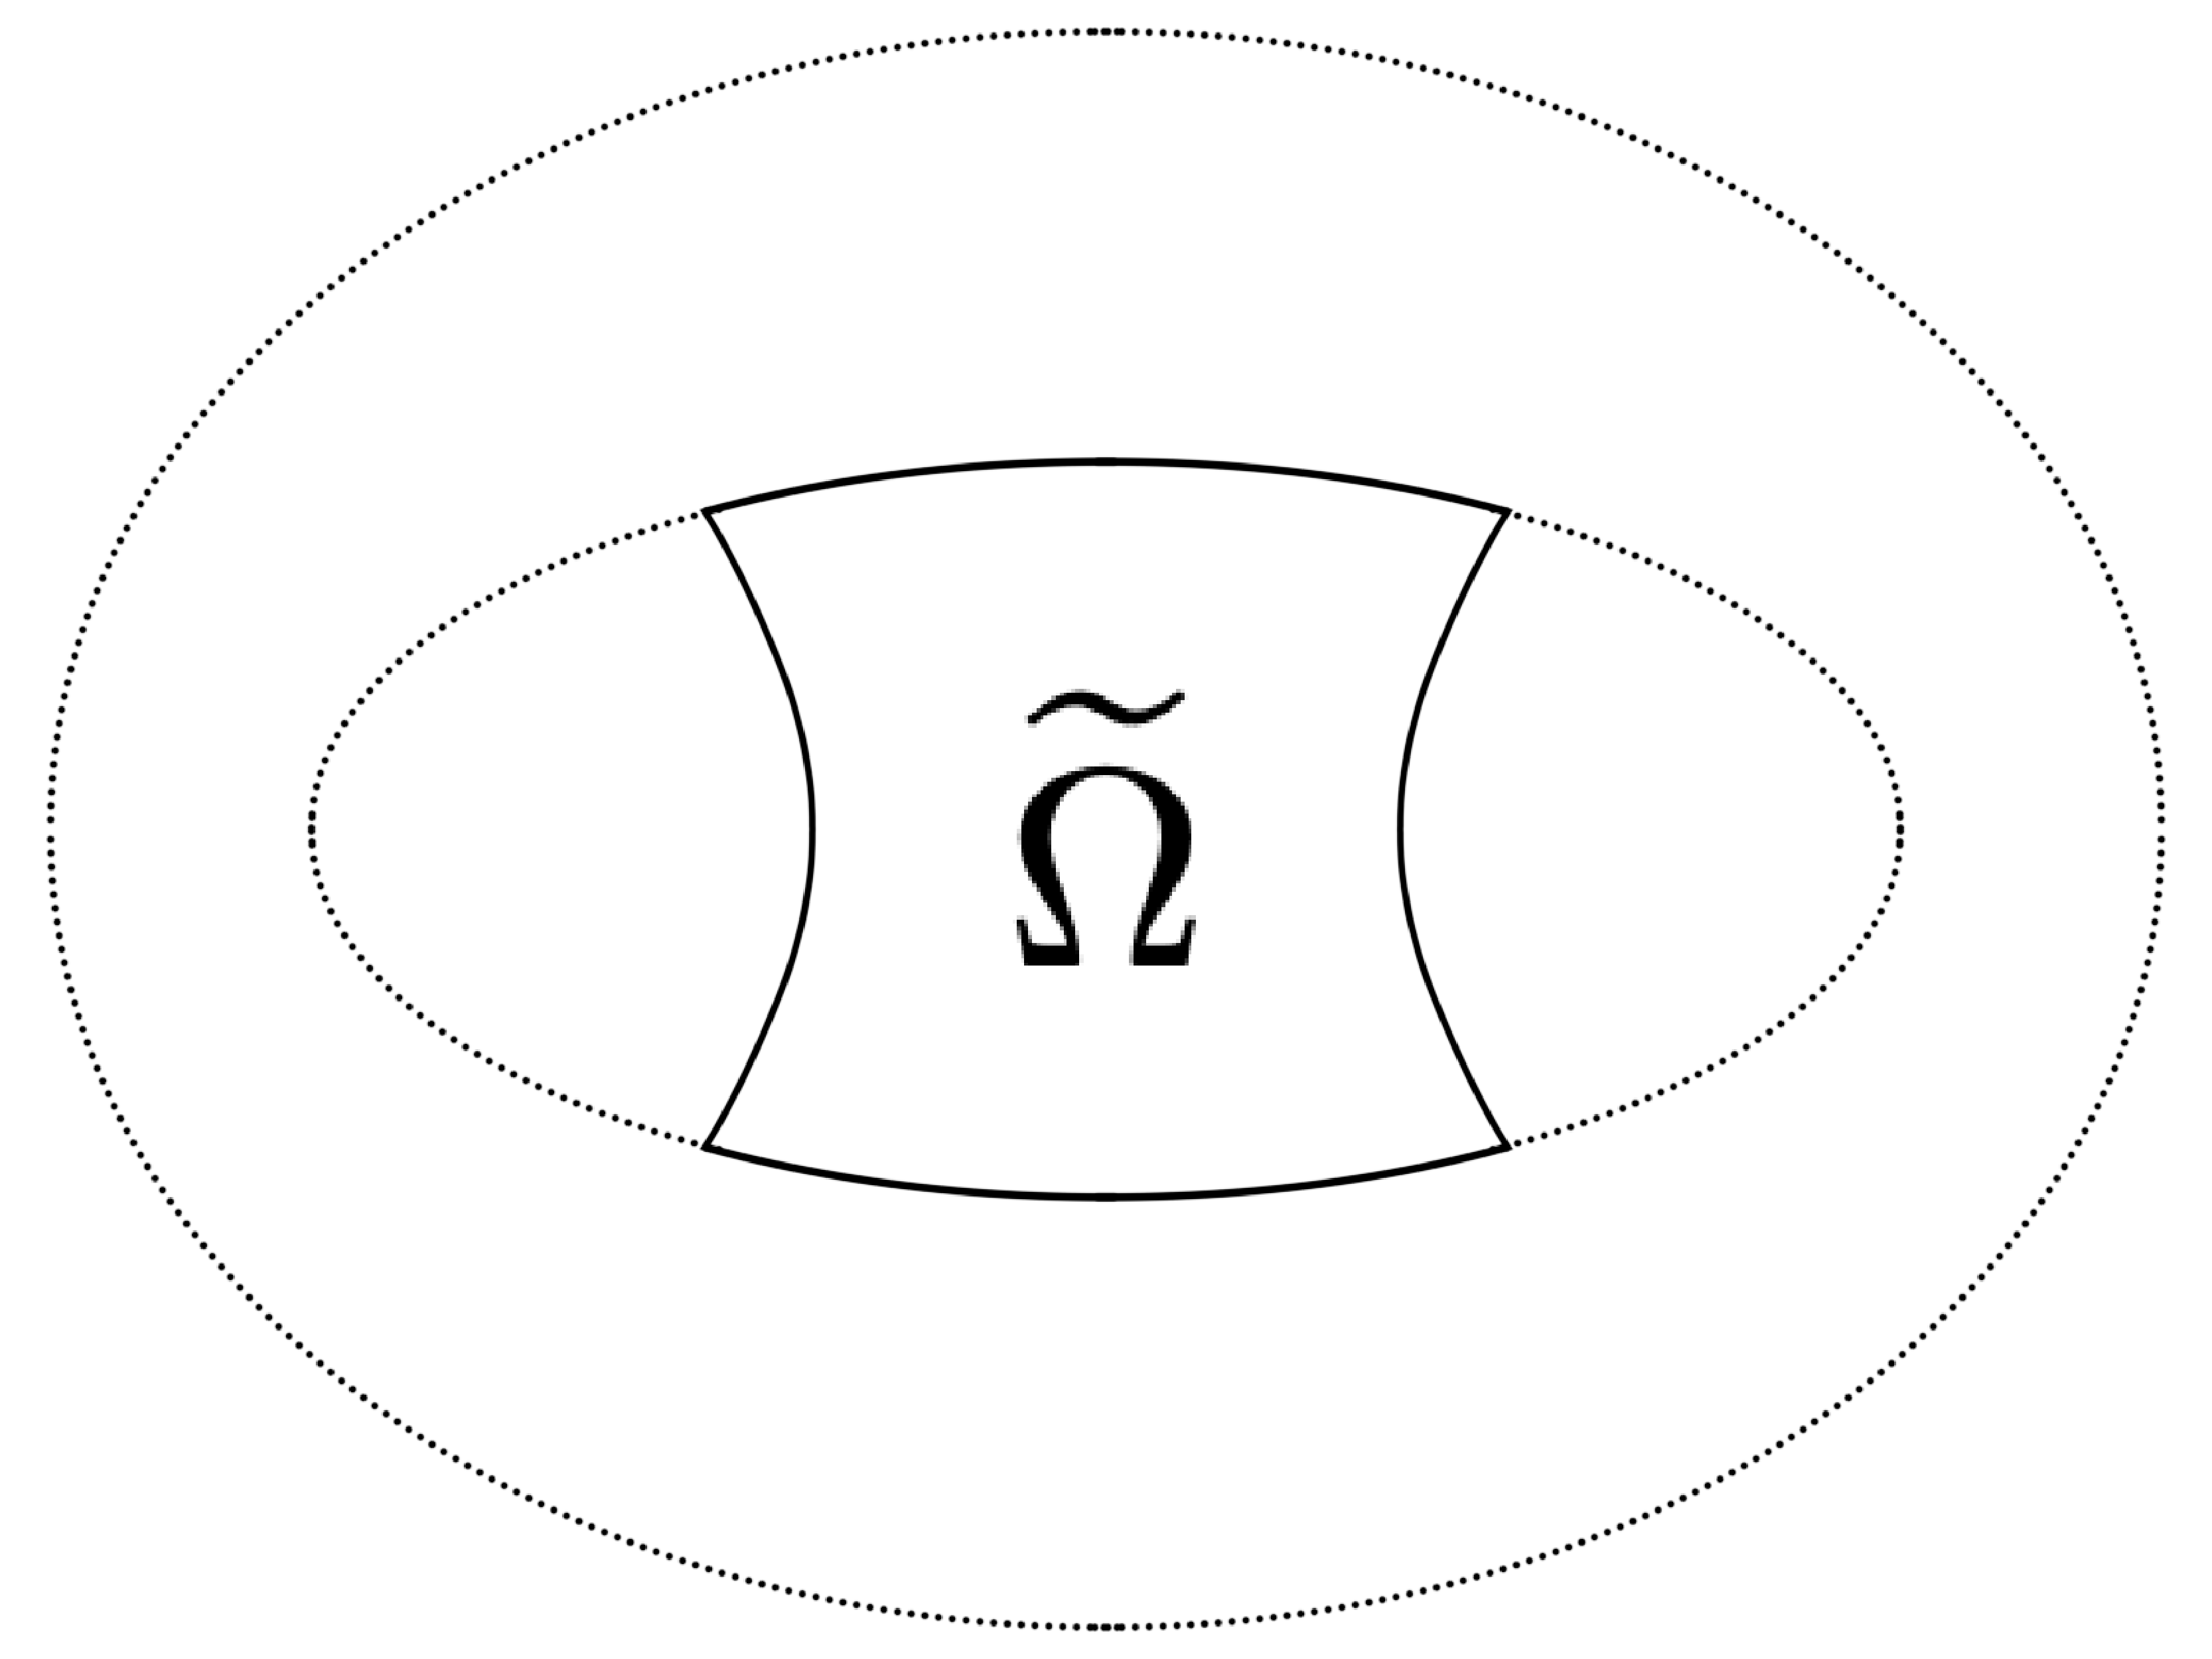
\includegraphics[width=0.8\linewidth]{images/section2/hyp_domain_example.pdf}
    \caption{Результирующая область $\widetilde{\Omega}$ для случая $D_3^2$.}
    \label{fig:pt9:_hyp_domain_example}
\endminipage\hfill
\minipage{0.45\textwidth}
\centering
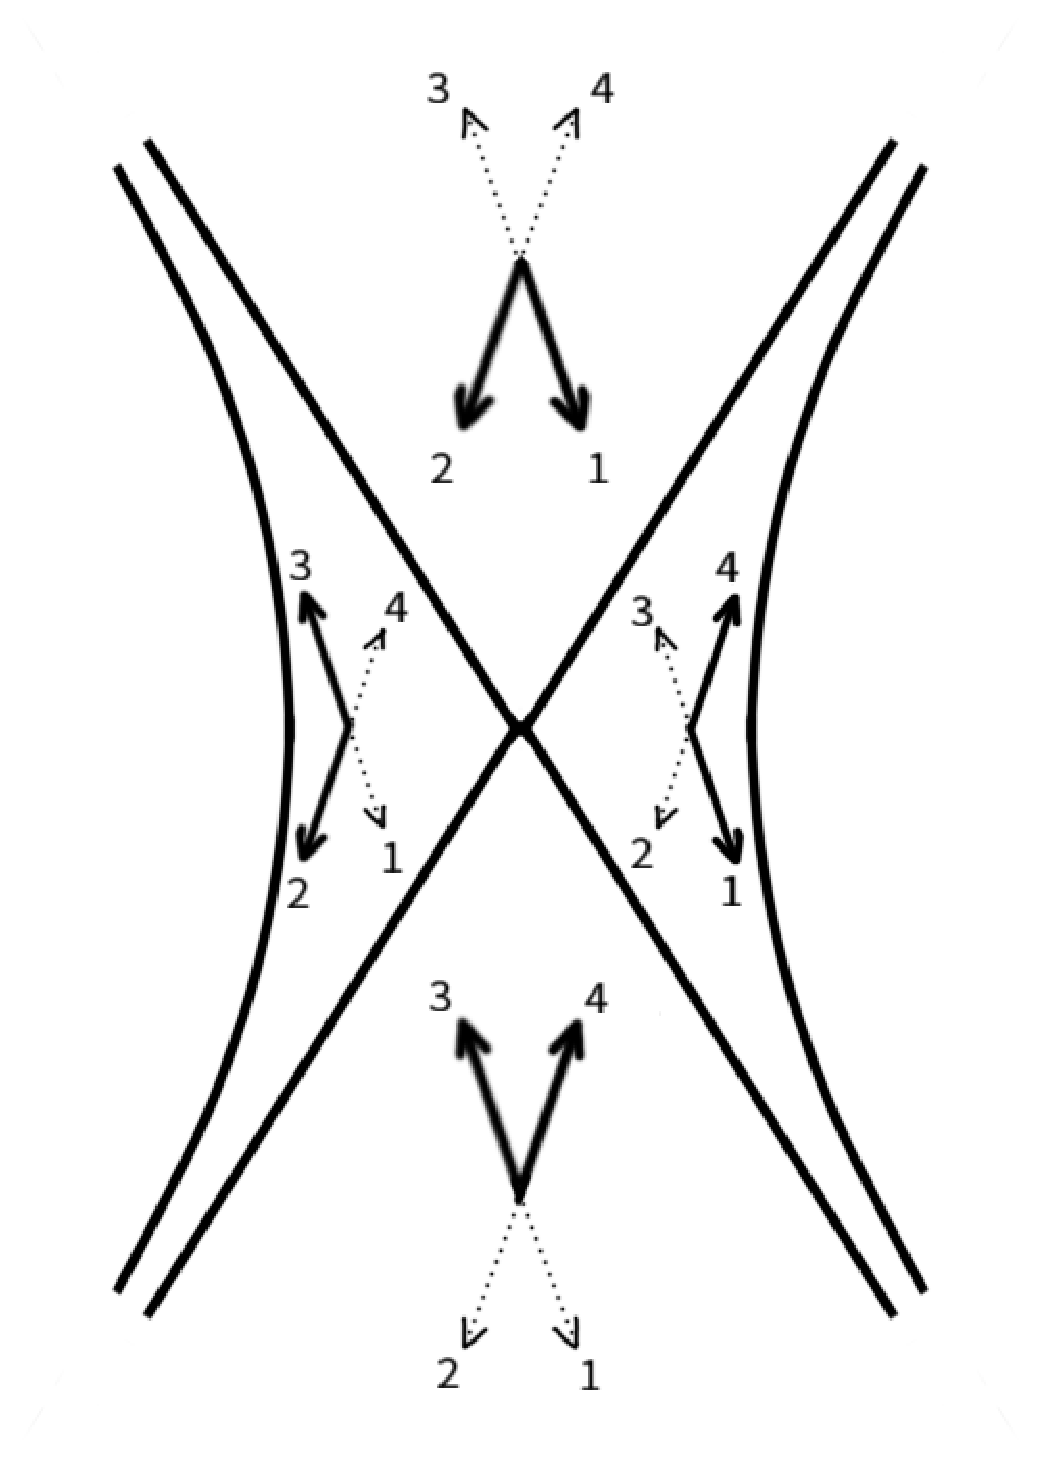
\includegraphics[width=0.65\linewidth]{images/section2/hyp_vectors_numbering.pdf}
    \caption{Направления векторов скорости $v_i$}
    \label{fig:pt9:_hyp_vectors_numbering}
\endminipage\hfill
\end{figure}

Граничные эллиптические дуги области $\widetilde{\Omega}_1$ склеиваются с одноименными эллиптическими дугами области $\widetilde{\Omega}_4$, аналогично для областей $\widetilde{\Omega}_2$, $\widetilde{\Omega}_3$.
Эти склейки дают нам две трубки.
Обе граничные гиперболы области $\widetilde{\Omega}_1$ отождествляются с соответствующими граничными гиперболами области $\widetilde{\Omega}_2$, аналогично для областей $\widetilde{\Omega}_3$ и $\widetilde{\Omega}_4$. Результатом склейки является один тор.

\medskip
\textbf{Случай $D_4^1$.} В этом случае проекция точки $(x, y, v_x, v_y)$, лежащей на поверхности $\Xi=\const$ при проекции $\pi$ заметает несвязную область, которая получается пересечением эллиптического кольца, ограниченного эллипсами $Q_{\lambda_1}$ и $Q_{0}$, и областью, содержащейся между ветвями гиперболы с параметром $\alpha_{out}$  (см. рис. \ref{fig:pt9:_d41_page}). 

Ясно, что определенная таким образом $\widetilde{\Omega}$ имеет две компоненты связности. Прообраз $\widetilde{\Omega}$ --- четыре листа $\widetilde{\Omega}_j, j=1, \ldots, 4$, где нумерация листов определена в соответствии с рис. \ref{fig:pt9:_hyp_vectors_numbering}. Каждый лист $\widetilde{\Omega}_j$ является  дизъюнктным объединением связных  листов $\widetilde{\Omega}_j^u \sqcup \widetilde{\Omega}_j^d$ (см. рис. \ref{fig:pt9:_d41_page}). 
%Упростим каждый лист склейки в соответствии с утверждением \ref{st:equivalent_borders} и получим рис. \ref{fig:pt9:_d41_page_simple}. 
Рассуждения, аналогичные рассуждениям предыдущего пункта, показывают, что для $i=1,\ldots, 4$ области $\widetilde{\Omega}_i^u$ склеиваются в один тор, а области $\widetilde{\Omega}_i^d$ --- в другой тор.

% повторяют склейки области $\widetilde{\Omega}$ в задаче $D_3^2$ и приводят к одному тору, аналогично результатом склейки четырех прямоугольников $\widetilde{\Omega}_i^d$ также является один тор.

\begin{figure}[!htb]
\centering
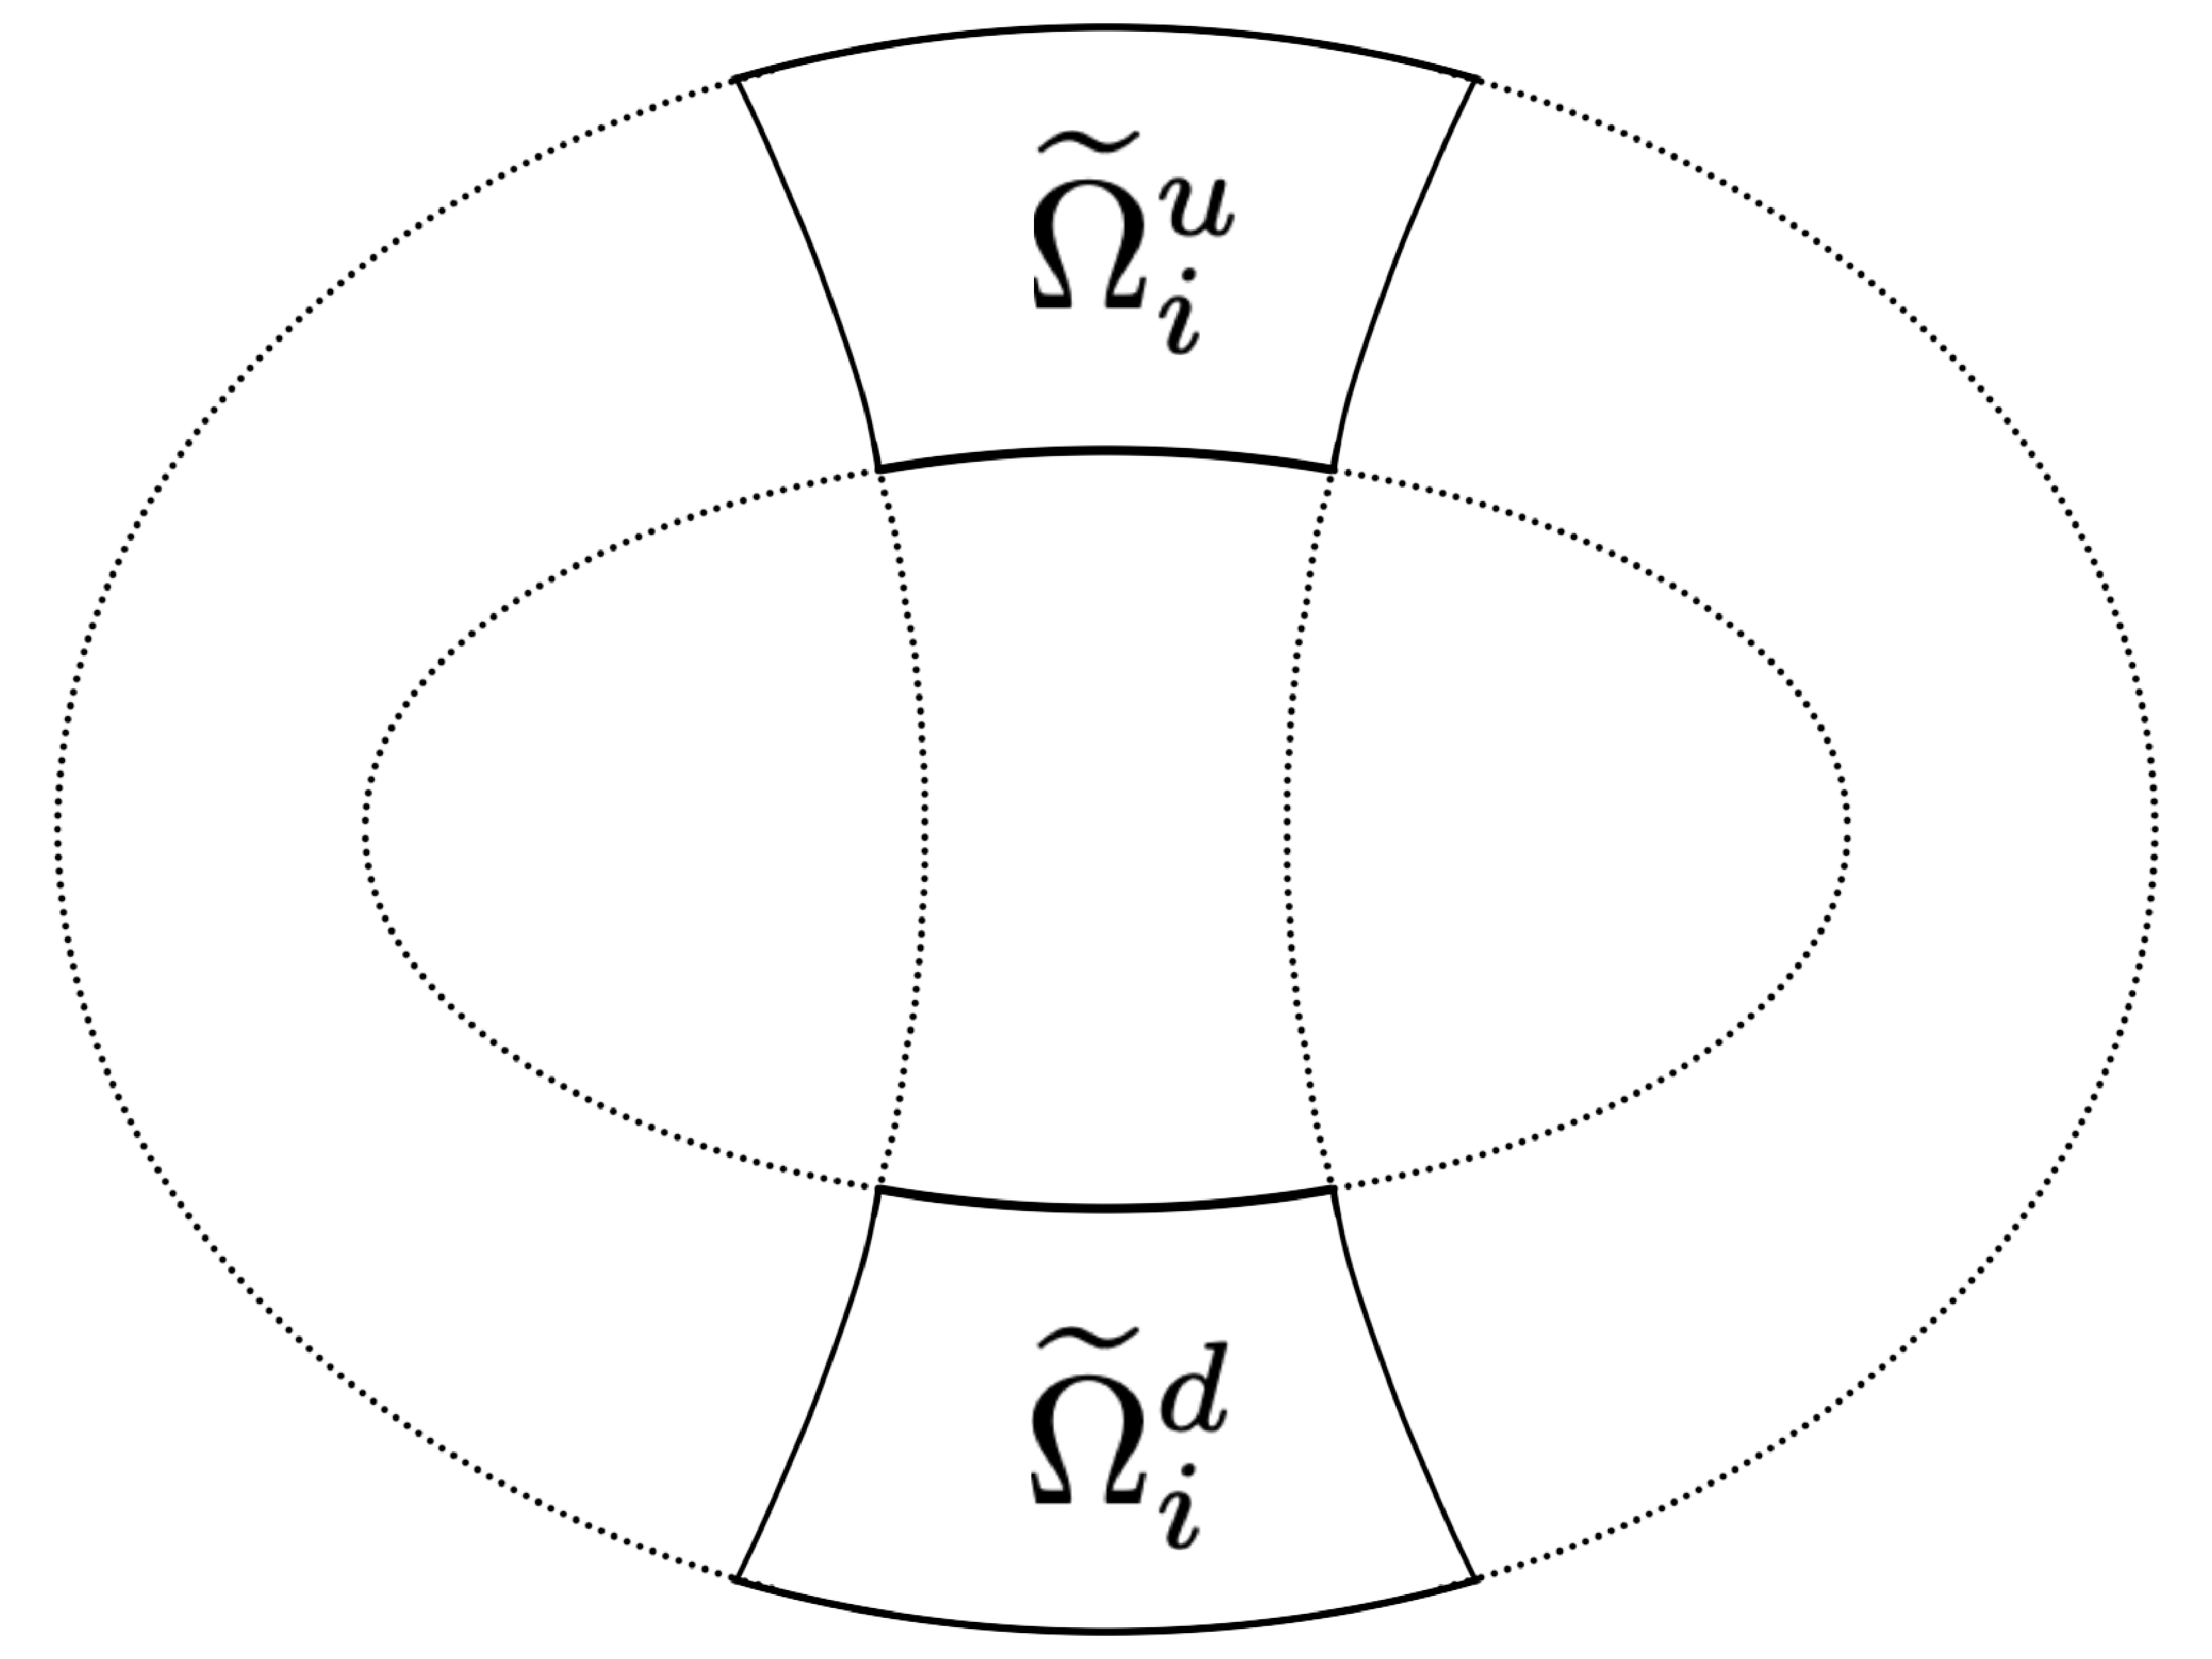
\includegraphics[width=0.35\linewidth]{images/section2/d41_page.pdf}
    \caption{Лист склейки  $\widetilde{\Omega}_i$  для случая $D_4^1$ состоит из двух областей.}
    \label{fig:pt9:_d41_page}
\end{figure}

\medskip
\textbf{Случай $D_1^2, D_1^3$. } 
Оба случая разбираются по одной схеме. 

Звенья и продолжения звеньев траектории, лежащие в $\Omega_{out}$, касаются гиперболы с параметром $\alpha_{out}$. Лежащие в $\Omega_{in}$ звенья и их продолжения касаются гиперболы с параметром $\alpha_{in}$.

Определим область $\widetilde{\Omega}_{in}$ как часть внутреннего эллипса $\Omega_{in}$, находящуюся между ветвей гиперболы $Q_{\alpha_{in}}$. Положим $\widetilde{\Omega}_{out}$ --- пересечение эллиптического кольца $\Omega_{out}$ с областью, лежащей между ветвями гиперболы с параметром $\alpha_{out}$; $\widetilde{\Omega}_{out}$ имеет две компоненты связности.

Проекция бильярдной траектории в эллиптической области заметает $\widetilde{\Omega} = \widetilde{\Omega}_{in} \cup \widetilde{\Omega}_{out}$ (см. рис.     \ref{fig:pt9:_img17}). Относительно проекции $\pi$ прообраз $\widetilde{\Omega}$ состоит из 4 листов $\widetilde{\Omega}_j, \ j=1, \ldots, 4$. 
Нумерацию листов снова сделаем в соответствии с рис. \ref{fig:pt9:_hyp_vectors_numbering}.

\begin{figure}[!htb]
\minipage{0.43\textwidth}
\centering
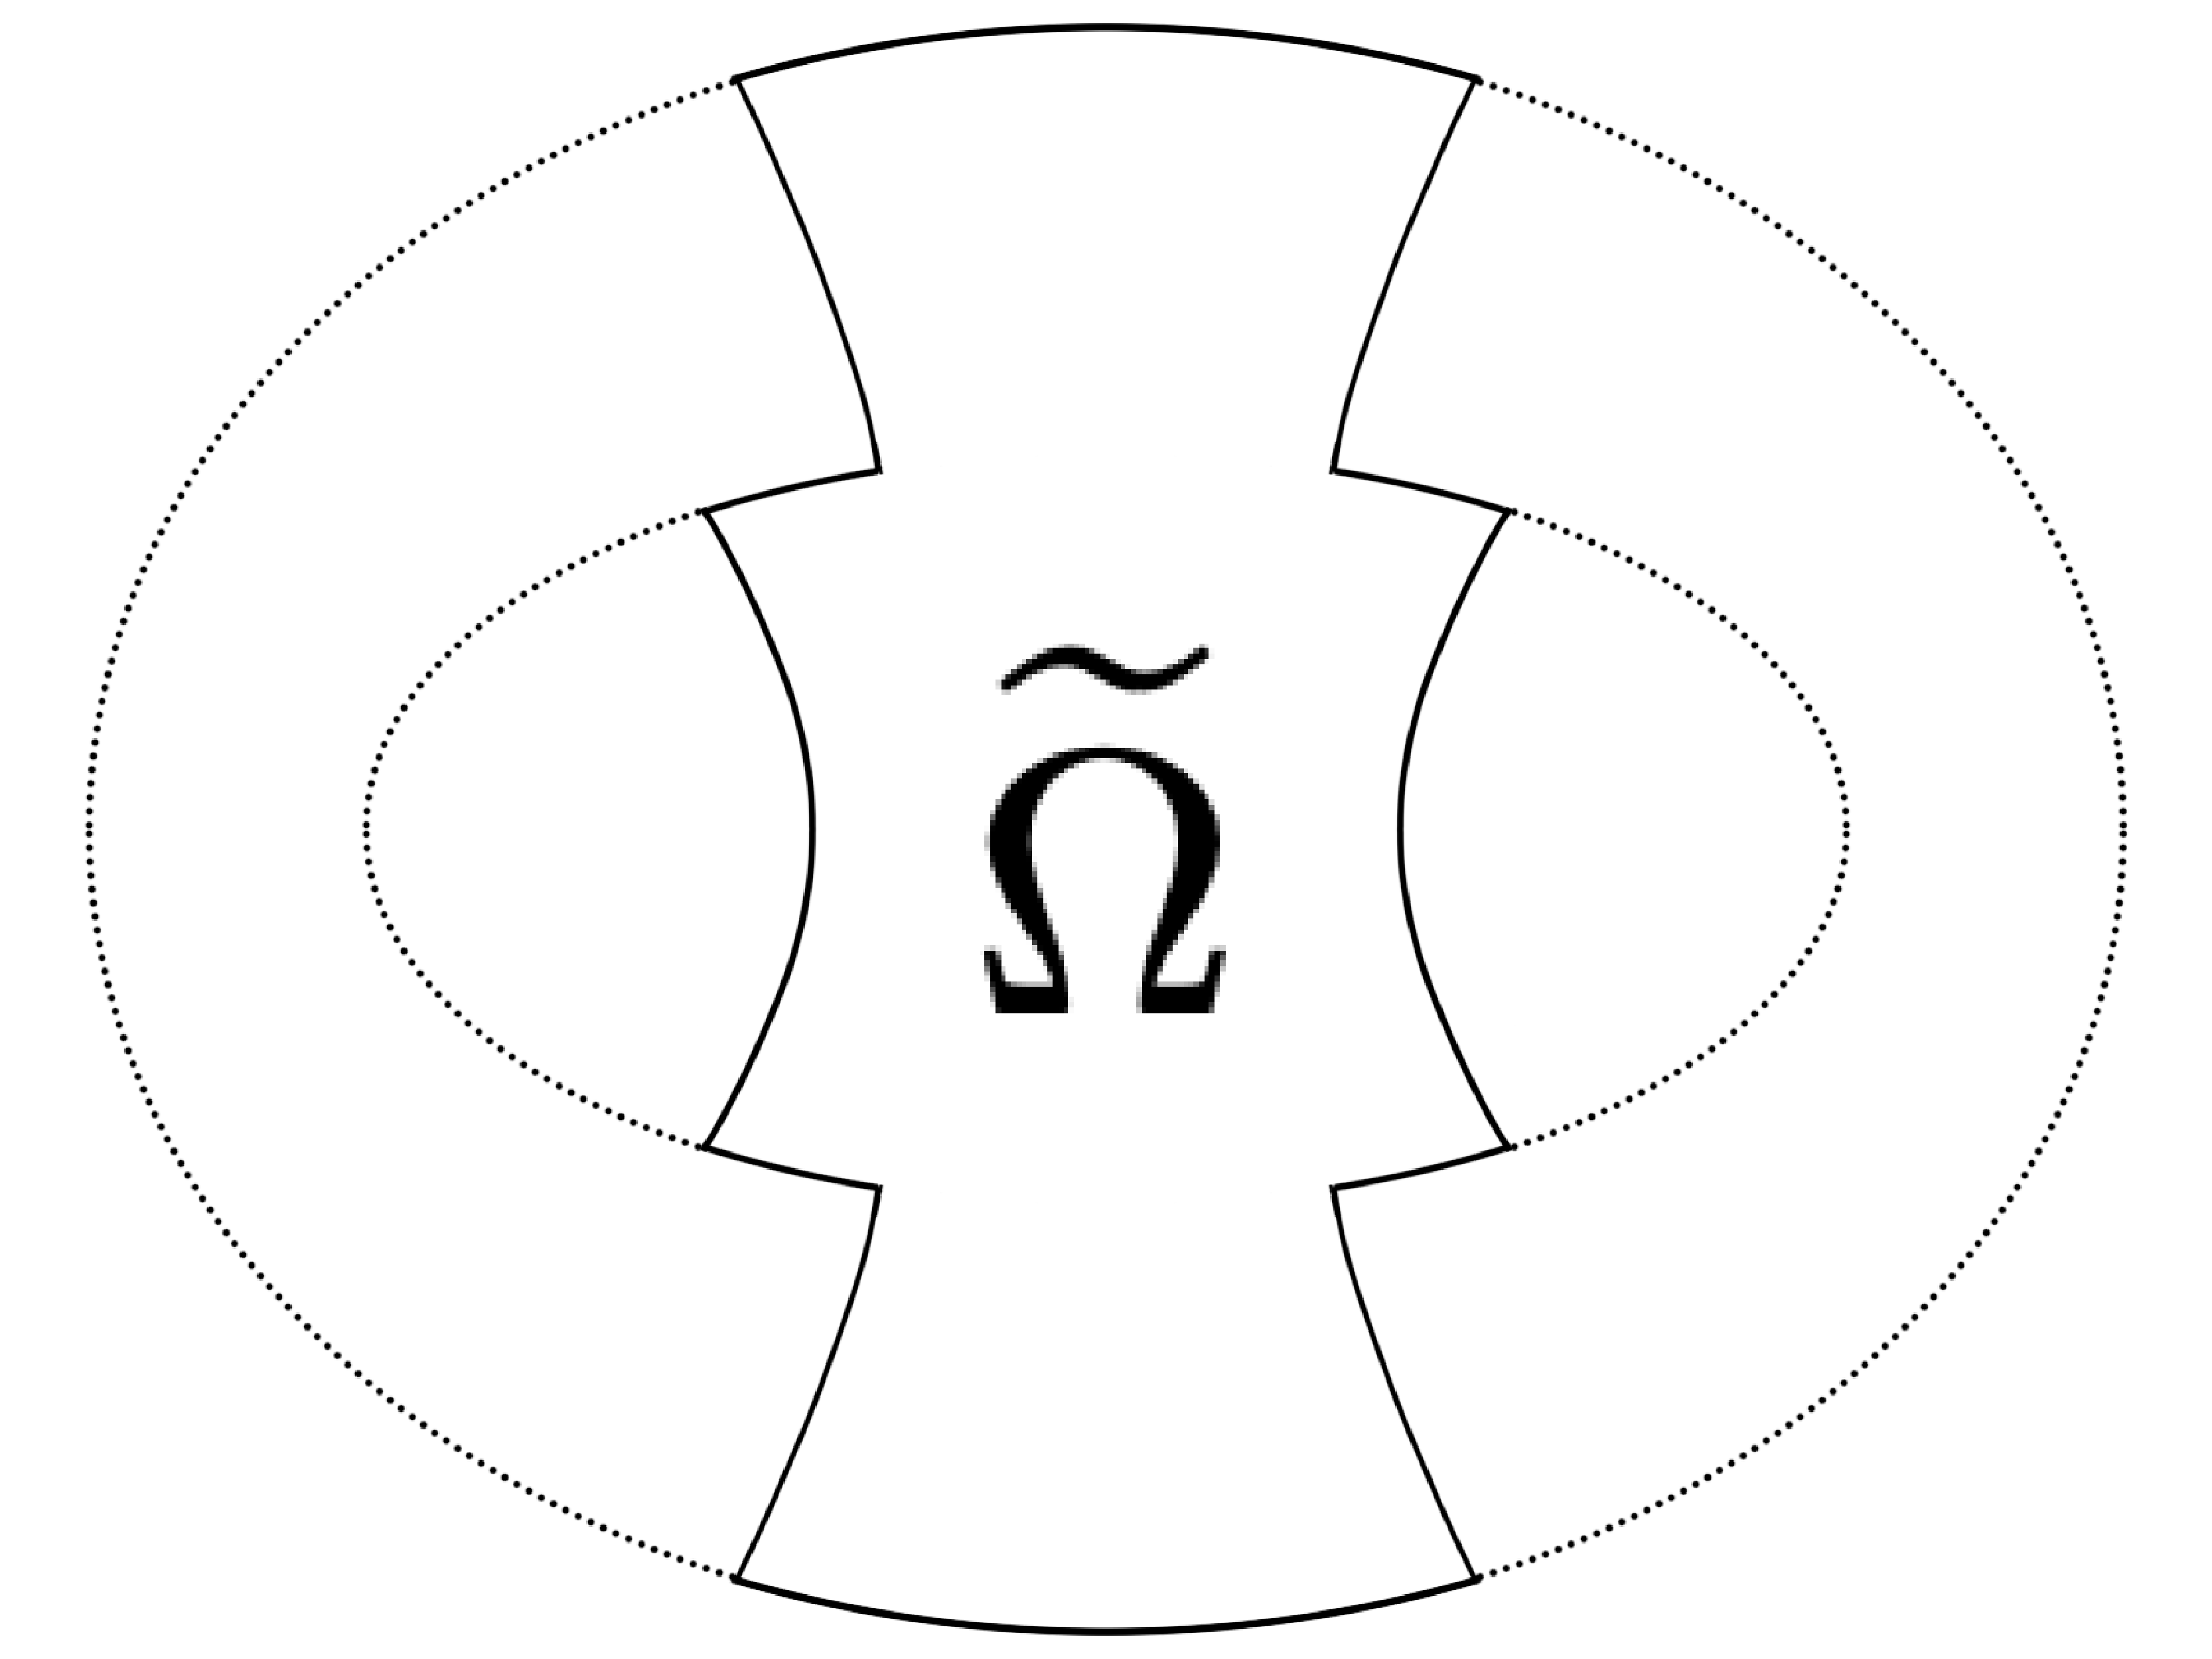
\includegraphics[width=0.7\linewidth]{images/section2/img17.pdf}
    \caption{Область $\widetilde{\Omega}$ для случая $D_1^2$.}
    \label{fig:pt9:_img17}
\endminipage\hfill
\minipage{0.42\textwidth}
\centering
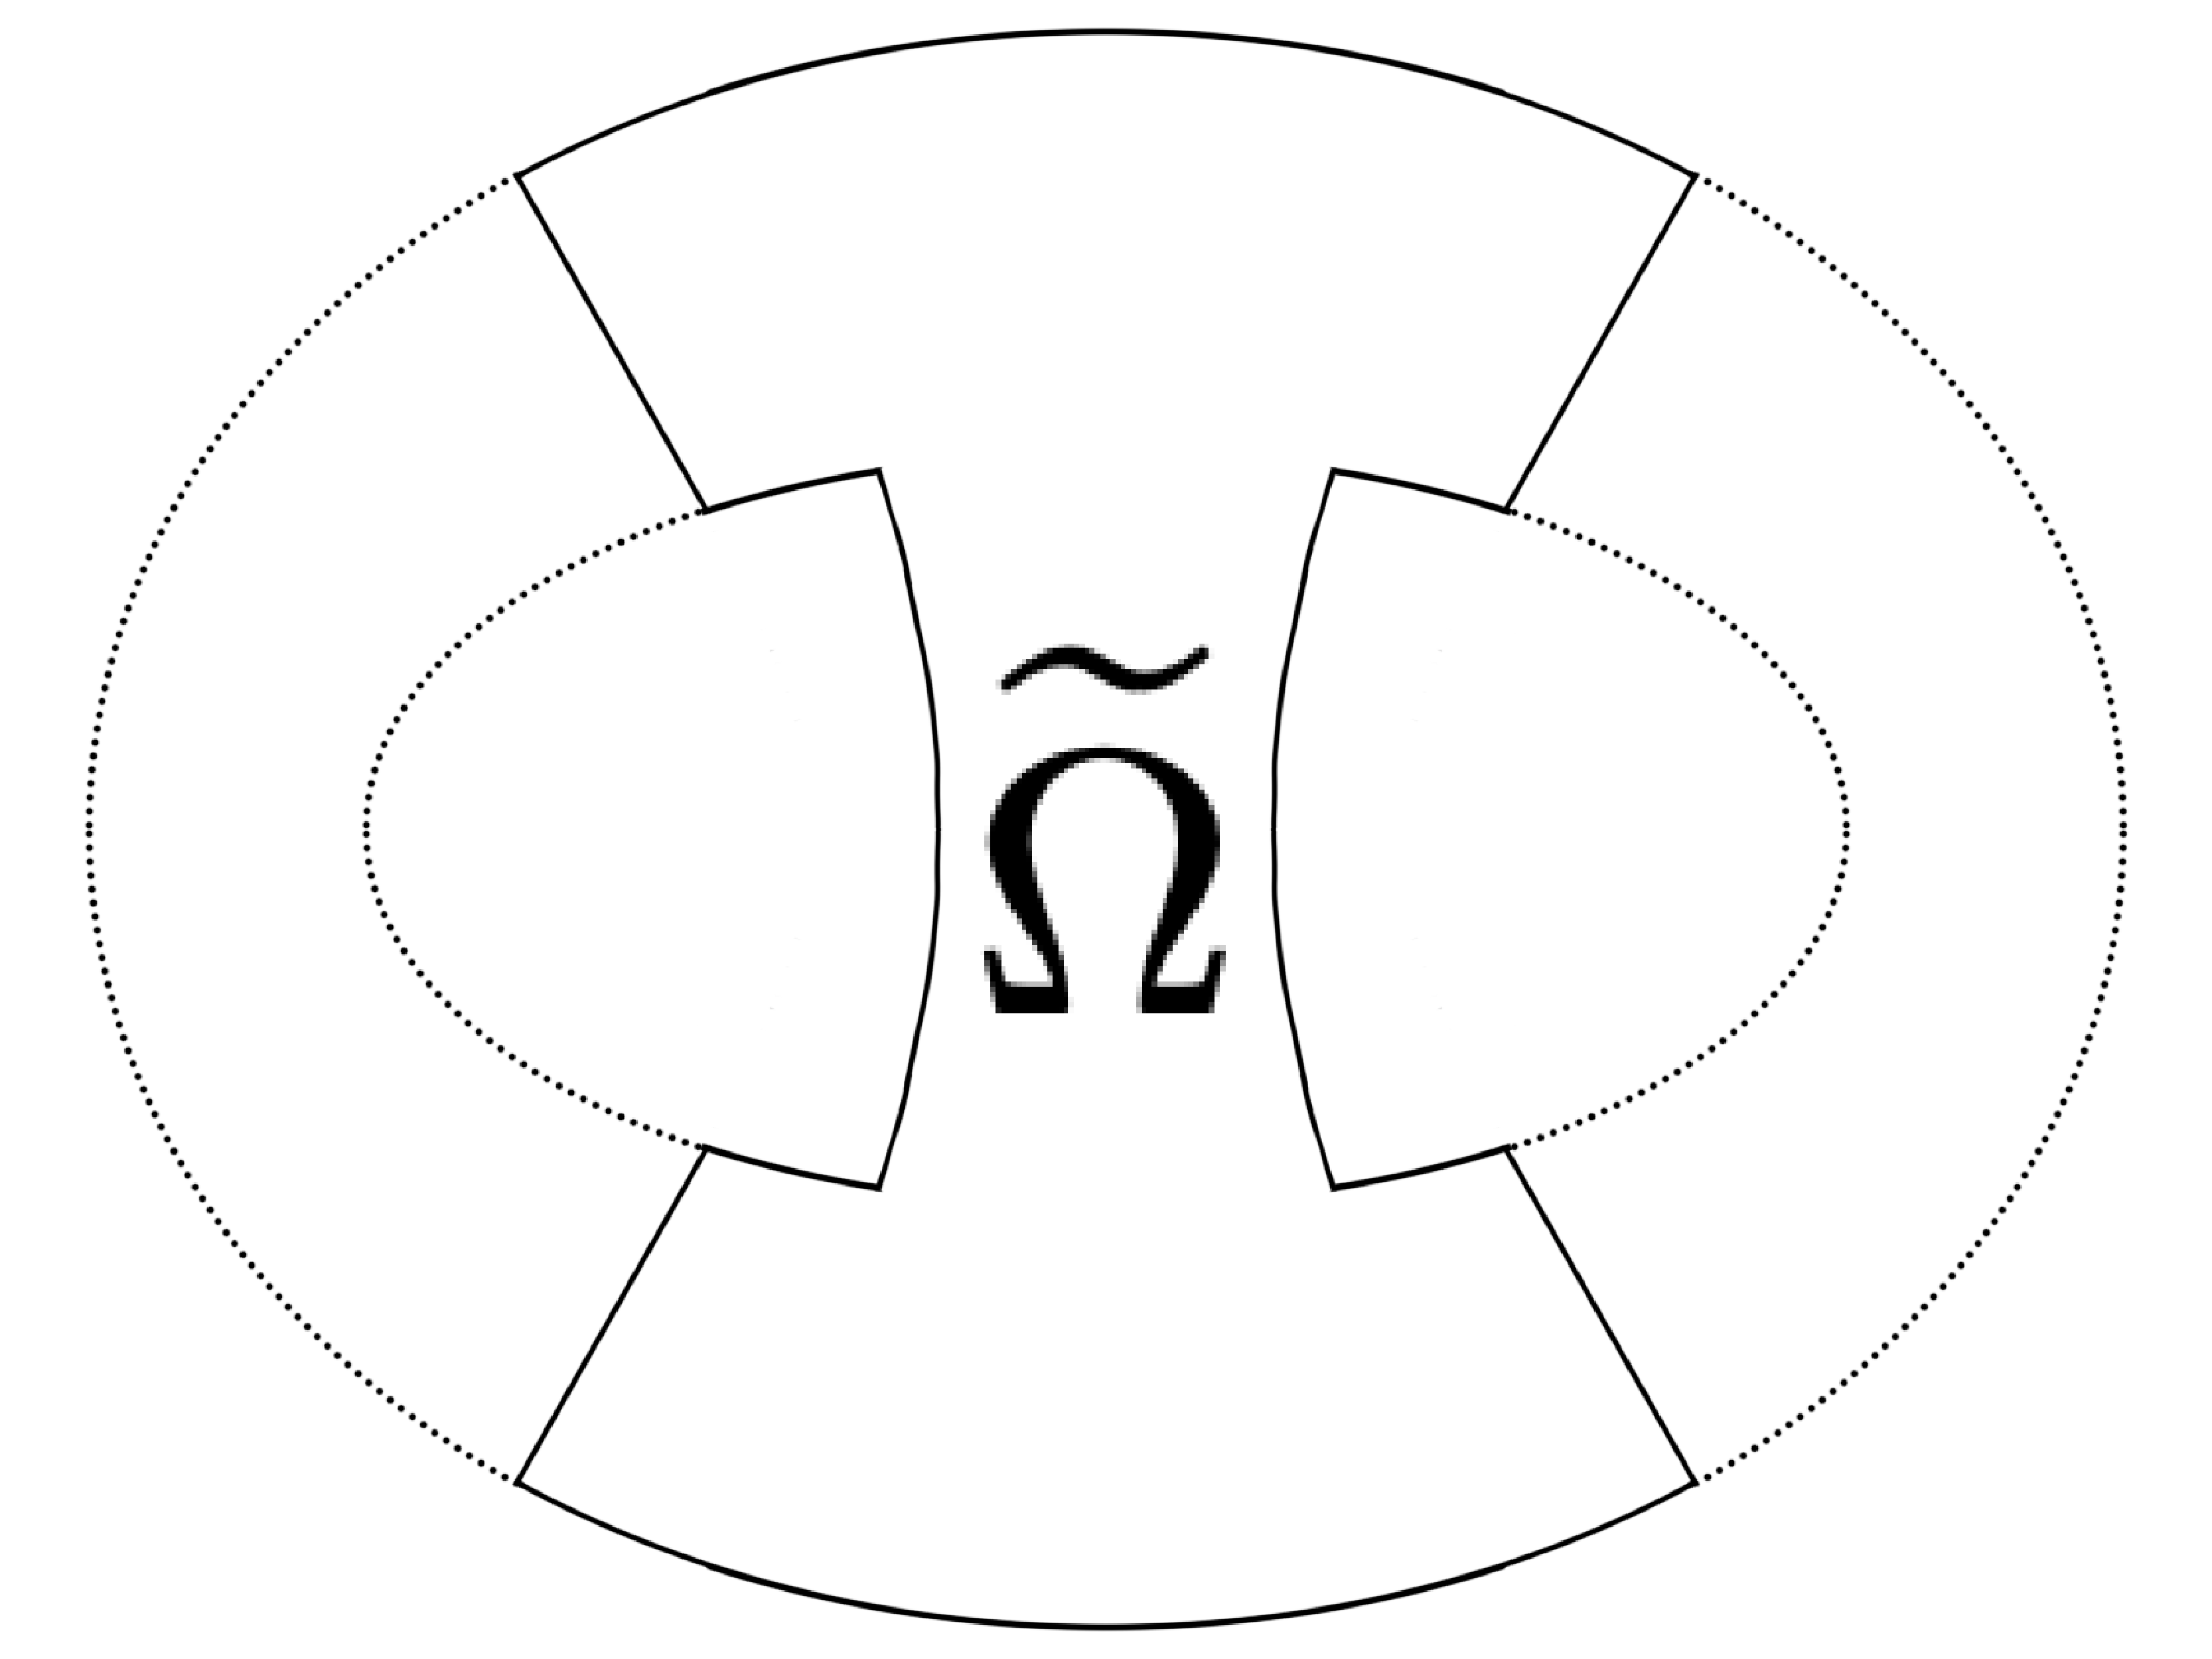
\includegraphics[width=0.7\linewidth]{images/section2/img18.pdf}
    \caption{Область $\widetilde{\Omega}$ для случая $D_1^3$.}
    \label{fig:pt9:_img18}
\endminipage\hfill
\end{figure}




Поверхность $\Xi=\const$ склеена из $\widetilde{\Omega}_1, \ldots, \widetilde{\Omega}_4$.
Шесть граничных эллиптических дуг области $\widetilde{\Omega}_1$ склеиваются с соответствующими граничными эллиптическими дугами области $\widetilde{\Omega}_4$. Аналогично для областей $\widetilde{\Omega}_2$ и $\widetilde{\Omega}_3$.
Результатом этих склеек являются две сферы с шестью дырками каждая.
Каждая дырка ограничивается двумя дугами, проектирующимися в одну граничную гиперболическую дугу области $\widetilde{\Omega}$.

Остается отождествить края этих дырок. Для этого заметим, что граничные гиперболические дуги области $\widetilde{\Omega}_1$ отождествляются с соответствующими граничными гиперболами области $\widetilde{\Omega}_2$, аналогичное справедливо для областей $\widetilde{\Omega}_3$ и $\widetilde{\Omega}_4$. Результатом этих склеек является сфера с пятью ручками. 

\medskip
\textbf{Случай $D_1^1$.}
Звенья траектории бильярда, лежащие в области $\Omega_{out}$, лежат на касательных к гиперболе с параметром $\alpha_{out}$, в то время как сегменты траектории, находящиеся в области $\Omega_{in}$, касаются эллипса с параметром $\alpha_{in}$. 

Определим область $\widetilde{\Omega}_{in} = \Omega_{in} \setminus \Omega_{\alpha_{in}}$ (эллиптическое кольцо), а область $\widetilde{\Omega}_{out}$ определим как пересечение эллиптического кольца $\Omega_{out}$ с областью, лежащей между ветвями гиперболы с параметром $\alpha_{out}$; $\widetilde{\Omega}_{out}$ имеет две компоненты связности
(см.  предыдущий случай): $\widetilde{\Omega}_{out} = \widetilde{\Omega}_{out}^u \sqcup \widetilde{\Omega}_{out}^d$.

Поверхность $\Xi = \const$ склеена из областей 
$\widetilde{\Omega}_{in, j}$, $\widetilde{\Omega}_{out, j}^u$,  $\widetilde{\Omega}_{out, j}^d, \ j=1, \ldots, 4$. Здесь листы  $\widetilde{\Omega}_{out, j}^u, \widetilde{\Omega}_{out, j}^d$ занумерованы в соответствии с рис. \ref{fig:pt9:_hyp_vectors_numbering}. Листы $\widetilde{\Omega}_{in, j}$ занумерованы в соответствии с правилом  \eqref{eq:ell_numeration}.

Области $\widetilde{\Omega}_{out, j}^u$ и $\widetilde{\Omega}_{in, j}$ отождествляются по общей граничной дуге, которую проекция $\pi$ отображает в дугу 
$\partial \widetilde{\Omega}_{out}^u \cap \partial \widetilde{\Omega}_{in}$.
В симметрично расположенную дугу эллипса в нижней полуплоскости проекция $\pi$ отображает граничные дуги, на которых отождествляются следующие пары областей: 
$\widetilde{\Omega}_{out, 1}^d$ с $\widetilde{\Omega}_{in, 3}$,
$\widetilde{\Omega}_{out, 3}^d$ с $\widetilde{\Omega}_{in, 1}$,
$\widetilde{\Omega}_{out, 2}^d$ с $\widetilde{\Omega}_{in, 4}$ и 
$\widetilde{\Omega}_{out, 4}^d$ с $\widetilde{\Omega}_{in, 2}$.

Таким образом, поверхность $\Xi = \const$ склеена из четырех листов:
$\widetilde{\Omega}_1 = \widetilde{\Omega}_{out, 1}^u \cup \widetilde{\Omega}_{in, 1} \cup \widetilde{\Omega}_{out, 3}^d$, 
$\widetilde{\Omega}_2 = \widetilde{\Omega}_{out, 2}^u \cup \widetilde{\Omega}_{in, 2} \cup \widetilde{\Omega}_{out, 4}^d$, 
$\widetilde{\Omega}_3 = \widetilde{\Omega}_{out, 3}^u \cup \widetilde{\Omega}_{in, 3} \cup \widetilde{\Omega}_{out, 1}^d$ и 
 $\widetilde{\Omega}_4 = \widetilde{\Omega}_{out, 4}^u \cup \widetilde{\Omega}_{in, 4} \cup \widetilde{\Omega}_{out, 2}^d$ (лист $\widetilde{\Omega}_1$ показан на рис. \ref{fig:pt9:_hyp_page}).
 \begin{figure}[!htb]
 \centering
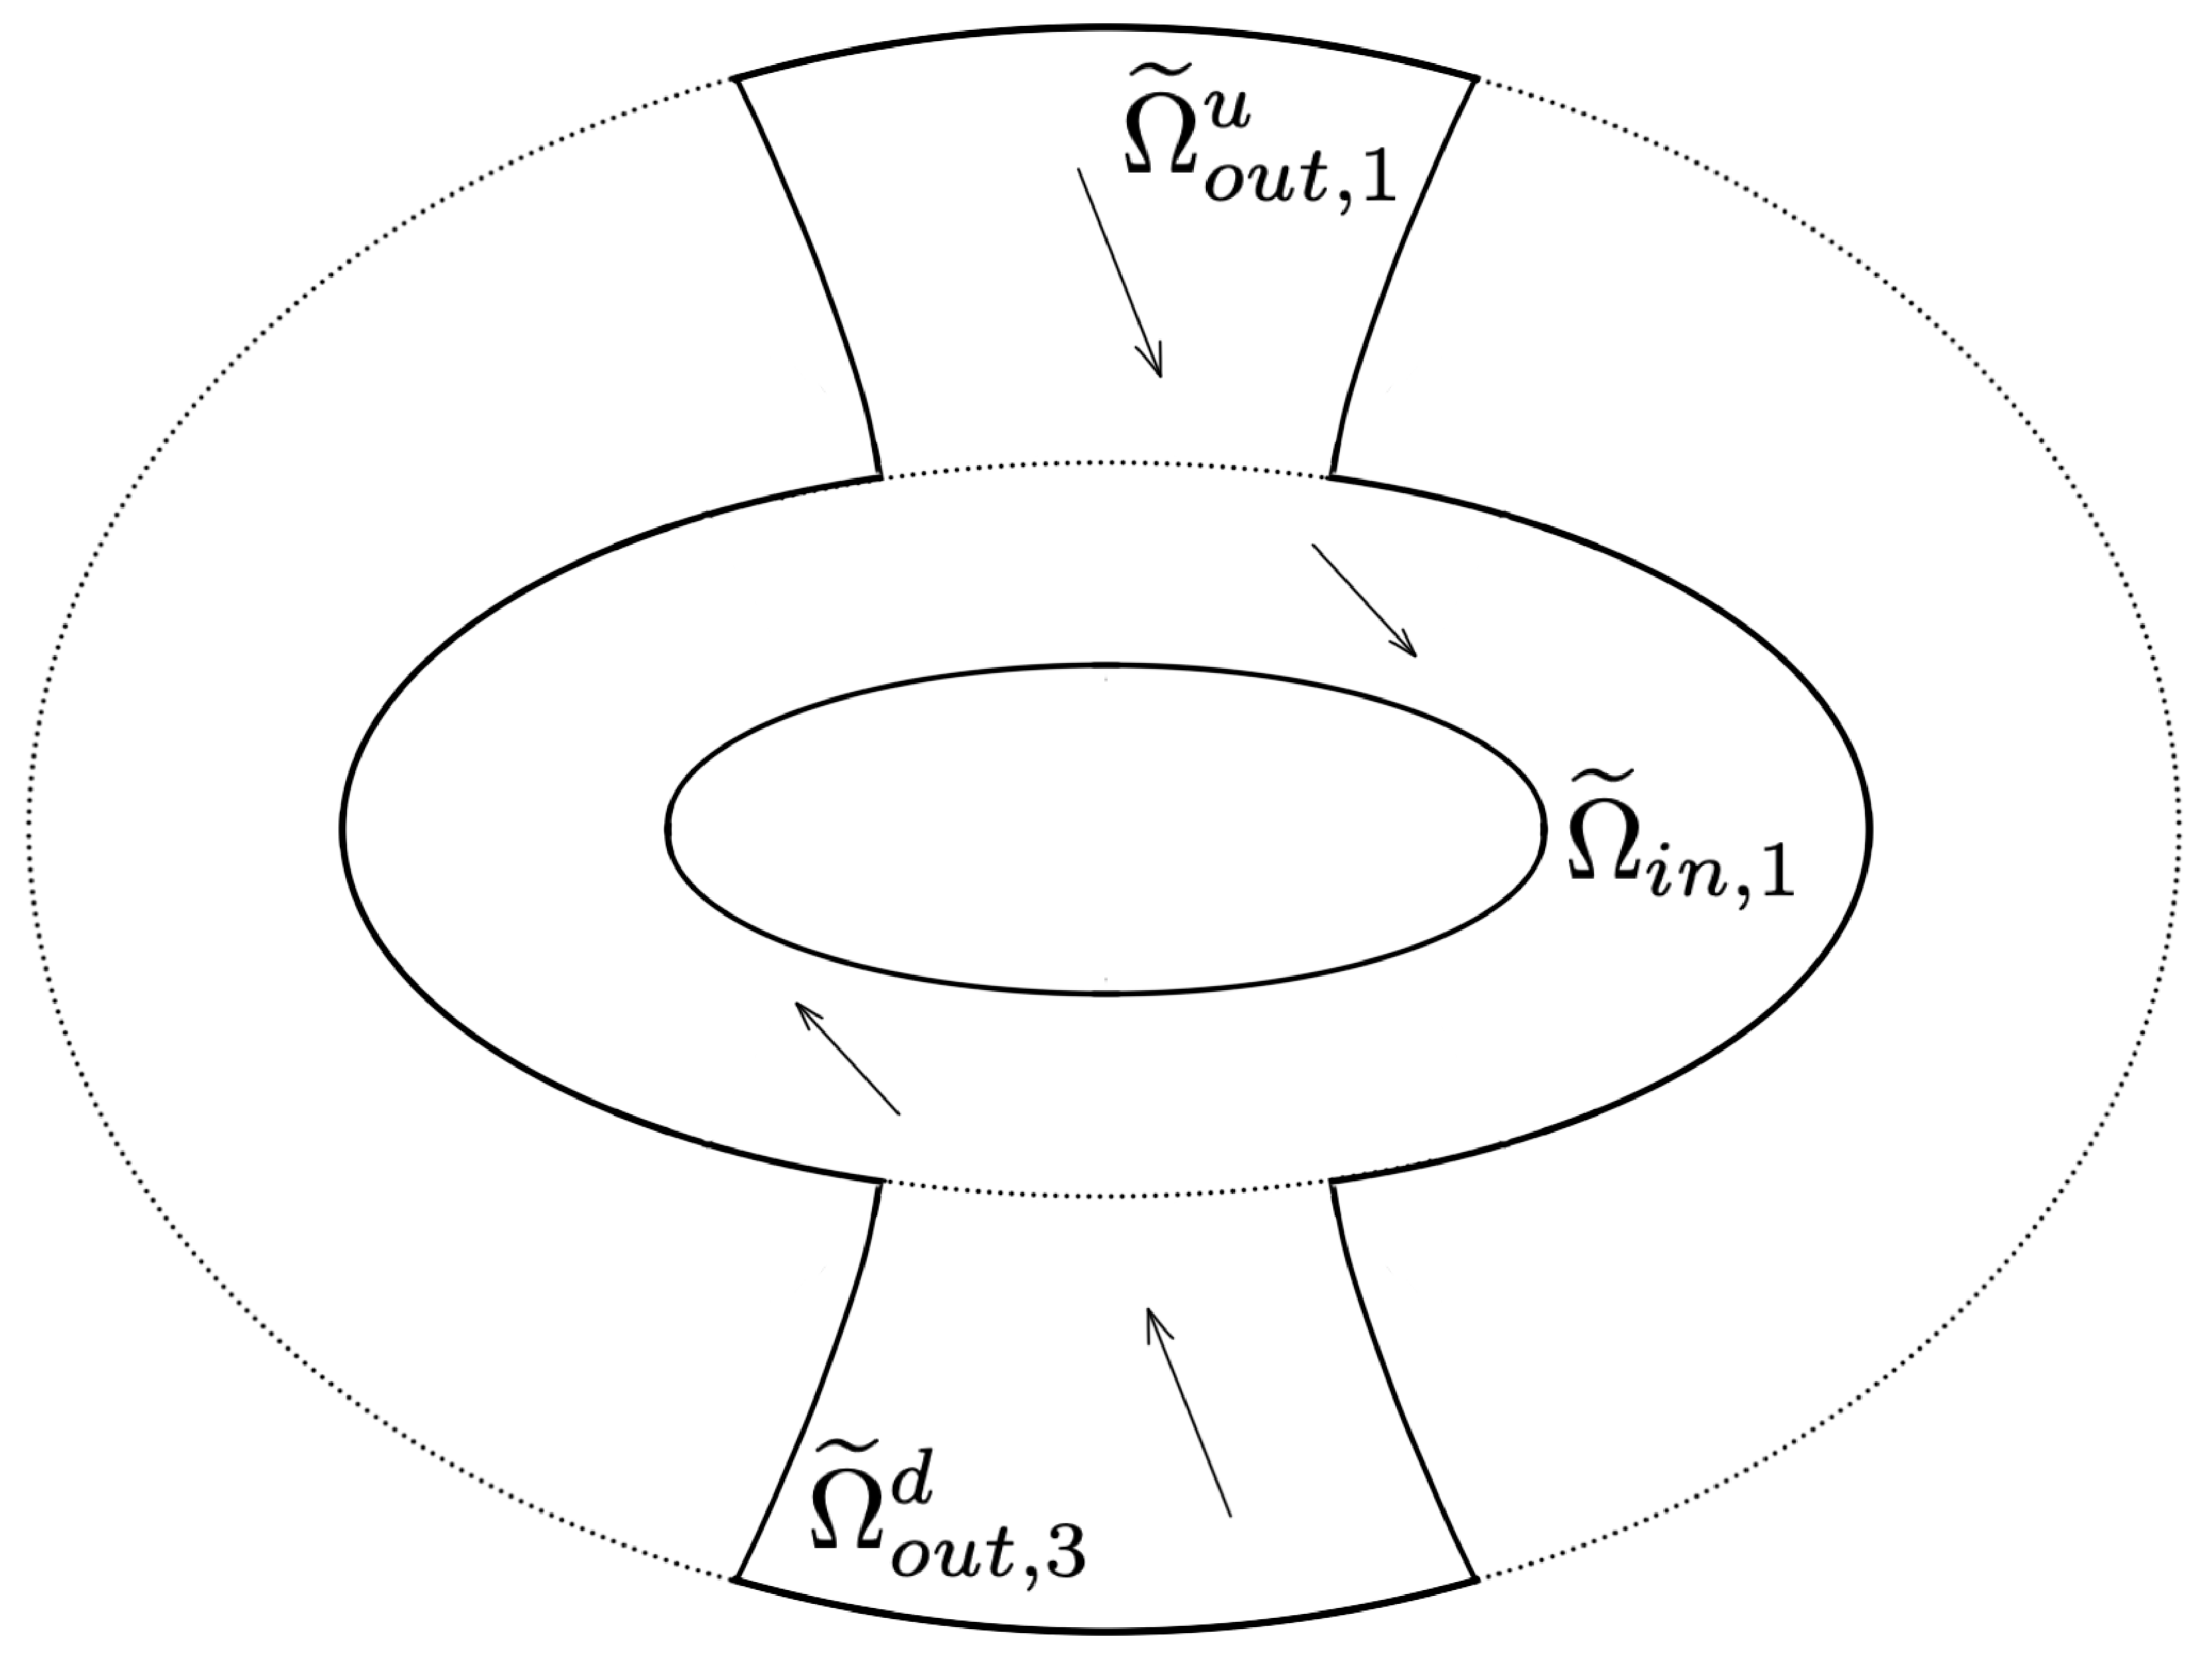
\includegraphics[width=0.4\linewidth]{images/section2/problems_vectors_2.pdf}
    \caption{Лист склейки $\widetilde{\Omega}_1$.}
    \label{fig:pt9:_hyp_page}
\end{figure}

 
Граничные эллиптические дуги области $\widetilde{\Omega}_1$  склеиваются с соответствующими эллиптическими дугами  области $\widetilde{\Omega}_4$, аналогично для областей $\widetilde{\Omega}_2$ и $\widetilde{\Omega}_3$. Результатом этих склеек являются два тора с четыремя дырками каждый. 
Каждая дырка ограничивается двумя дугами, проектирующимися в одну граничную гиперболическую дугу области $\widetilde{\Omega} = \widetilde{\Omega}_{in} \cup \widetilde{\Omega}_{out}$.

Остается отождествить края этих дырок. Для этого заметим, что граничные гиперболические дуги области $\widetilde{\Omega}_1$ отождествляются с одноименными граничными гиперболами области $\widetilde{\Omega}_2$, аналогичное справедливо для областей $\widetilde{\Omega}_3$ и $\widetilde{\Omega}_4$. Результатом этих склеек является сфера с пятью ручками. 

\textbf{Случай $D_1^6$}.
Продолжения звеньев бильярдной траектории, лежащие в $\Omega_{out}$, касаются эллипса с параметром $\alpha_{out}$, а сегменты траектории, находящиеся в $\Omega_{in}$, касаются гиперболы с параметром $\alpha_{in}$. 

Определим область $\widetilde{\Omega}_{in}$ как пересечение эллипса $\Omega_{in}$ и области, лежащей между двумя ветвями гиперболы с параметром $\alpha_{in}$.
Поверхность  $\Xi = \const$ проектируется на объединение $\widetilde{\Omega}_{in} \cup \Omega_{out}$. 
Каждой внутренней точке этой области соответствуют четыре точки-прообраза на поверхности $\Xi = \const$.
Тем самым, поверхность $\Xi = \const$ склеена из областей $\widetilde{\Omega}_{in, j}, \Omega_{out, j}, \ j=1,\ldots,4$.
Здесь области $\Omega_{out, j}$ нумеруются в соответствии с правилом \eqref{eq:ell_numeration}, а области $\widetilde{\Omega}_{in, j}$ нумеруются согласно рис. \ref{fig:pt9:_hyp_vectors_numbering}.


В силу закона преломления $(\ast)$ области $\widetilde{\Omega}_{in, j}$ и $\Omega_{out, j}$ для каждого $j=1,\ldots, 4$ отождествляются по общему участку границы, который проекция $\pi$ отображает в дугу эллипса $Q_{\lambda_1}$, а именно, в дугу $\partial \widetilde{\Omega}_{in} \cap \partial \Omega_{out}$, находящуюся в верхней полуплоскости.
В симметричную ей дугу в нижней полуплоскости проектируются общие участки границы для областей $\widetilde{\Omega}_{in, 1}$ и $\Omega_{out, 3}$ в силу того же закона $(\ast)$. Аналогично отождествляются области $\widetilde{\Omega}_{in, 2}$ и $\Omega_{out, 4}$, $\widetilde{\Omega}_{in, 3}$ и $\Omega_{out, 1}$, а также $\widetilde{\Omega}_{in, 4}$ и $\Omega_{out, 2}$.

Определим листы $\widetilde{\Omega}_j$, $j=1, \ldots, 4$ (пример см. рис. \ref{fig:pt9:_ell_and_hyp_2}) следующим образом: 
$\widetilde{\Omega}_j = \widetilde{\Omega}_{in, j} \cup \Omega_{out, j}$, где объединение листов осуществляется по общей дуге, проецирующейся на верхнюю дугу эллипса $Q_{\lambda_1}$.

\begin{figure}[!htb]
\minipage{0.4\textwidth}
\centering
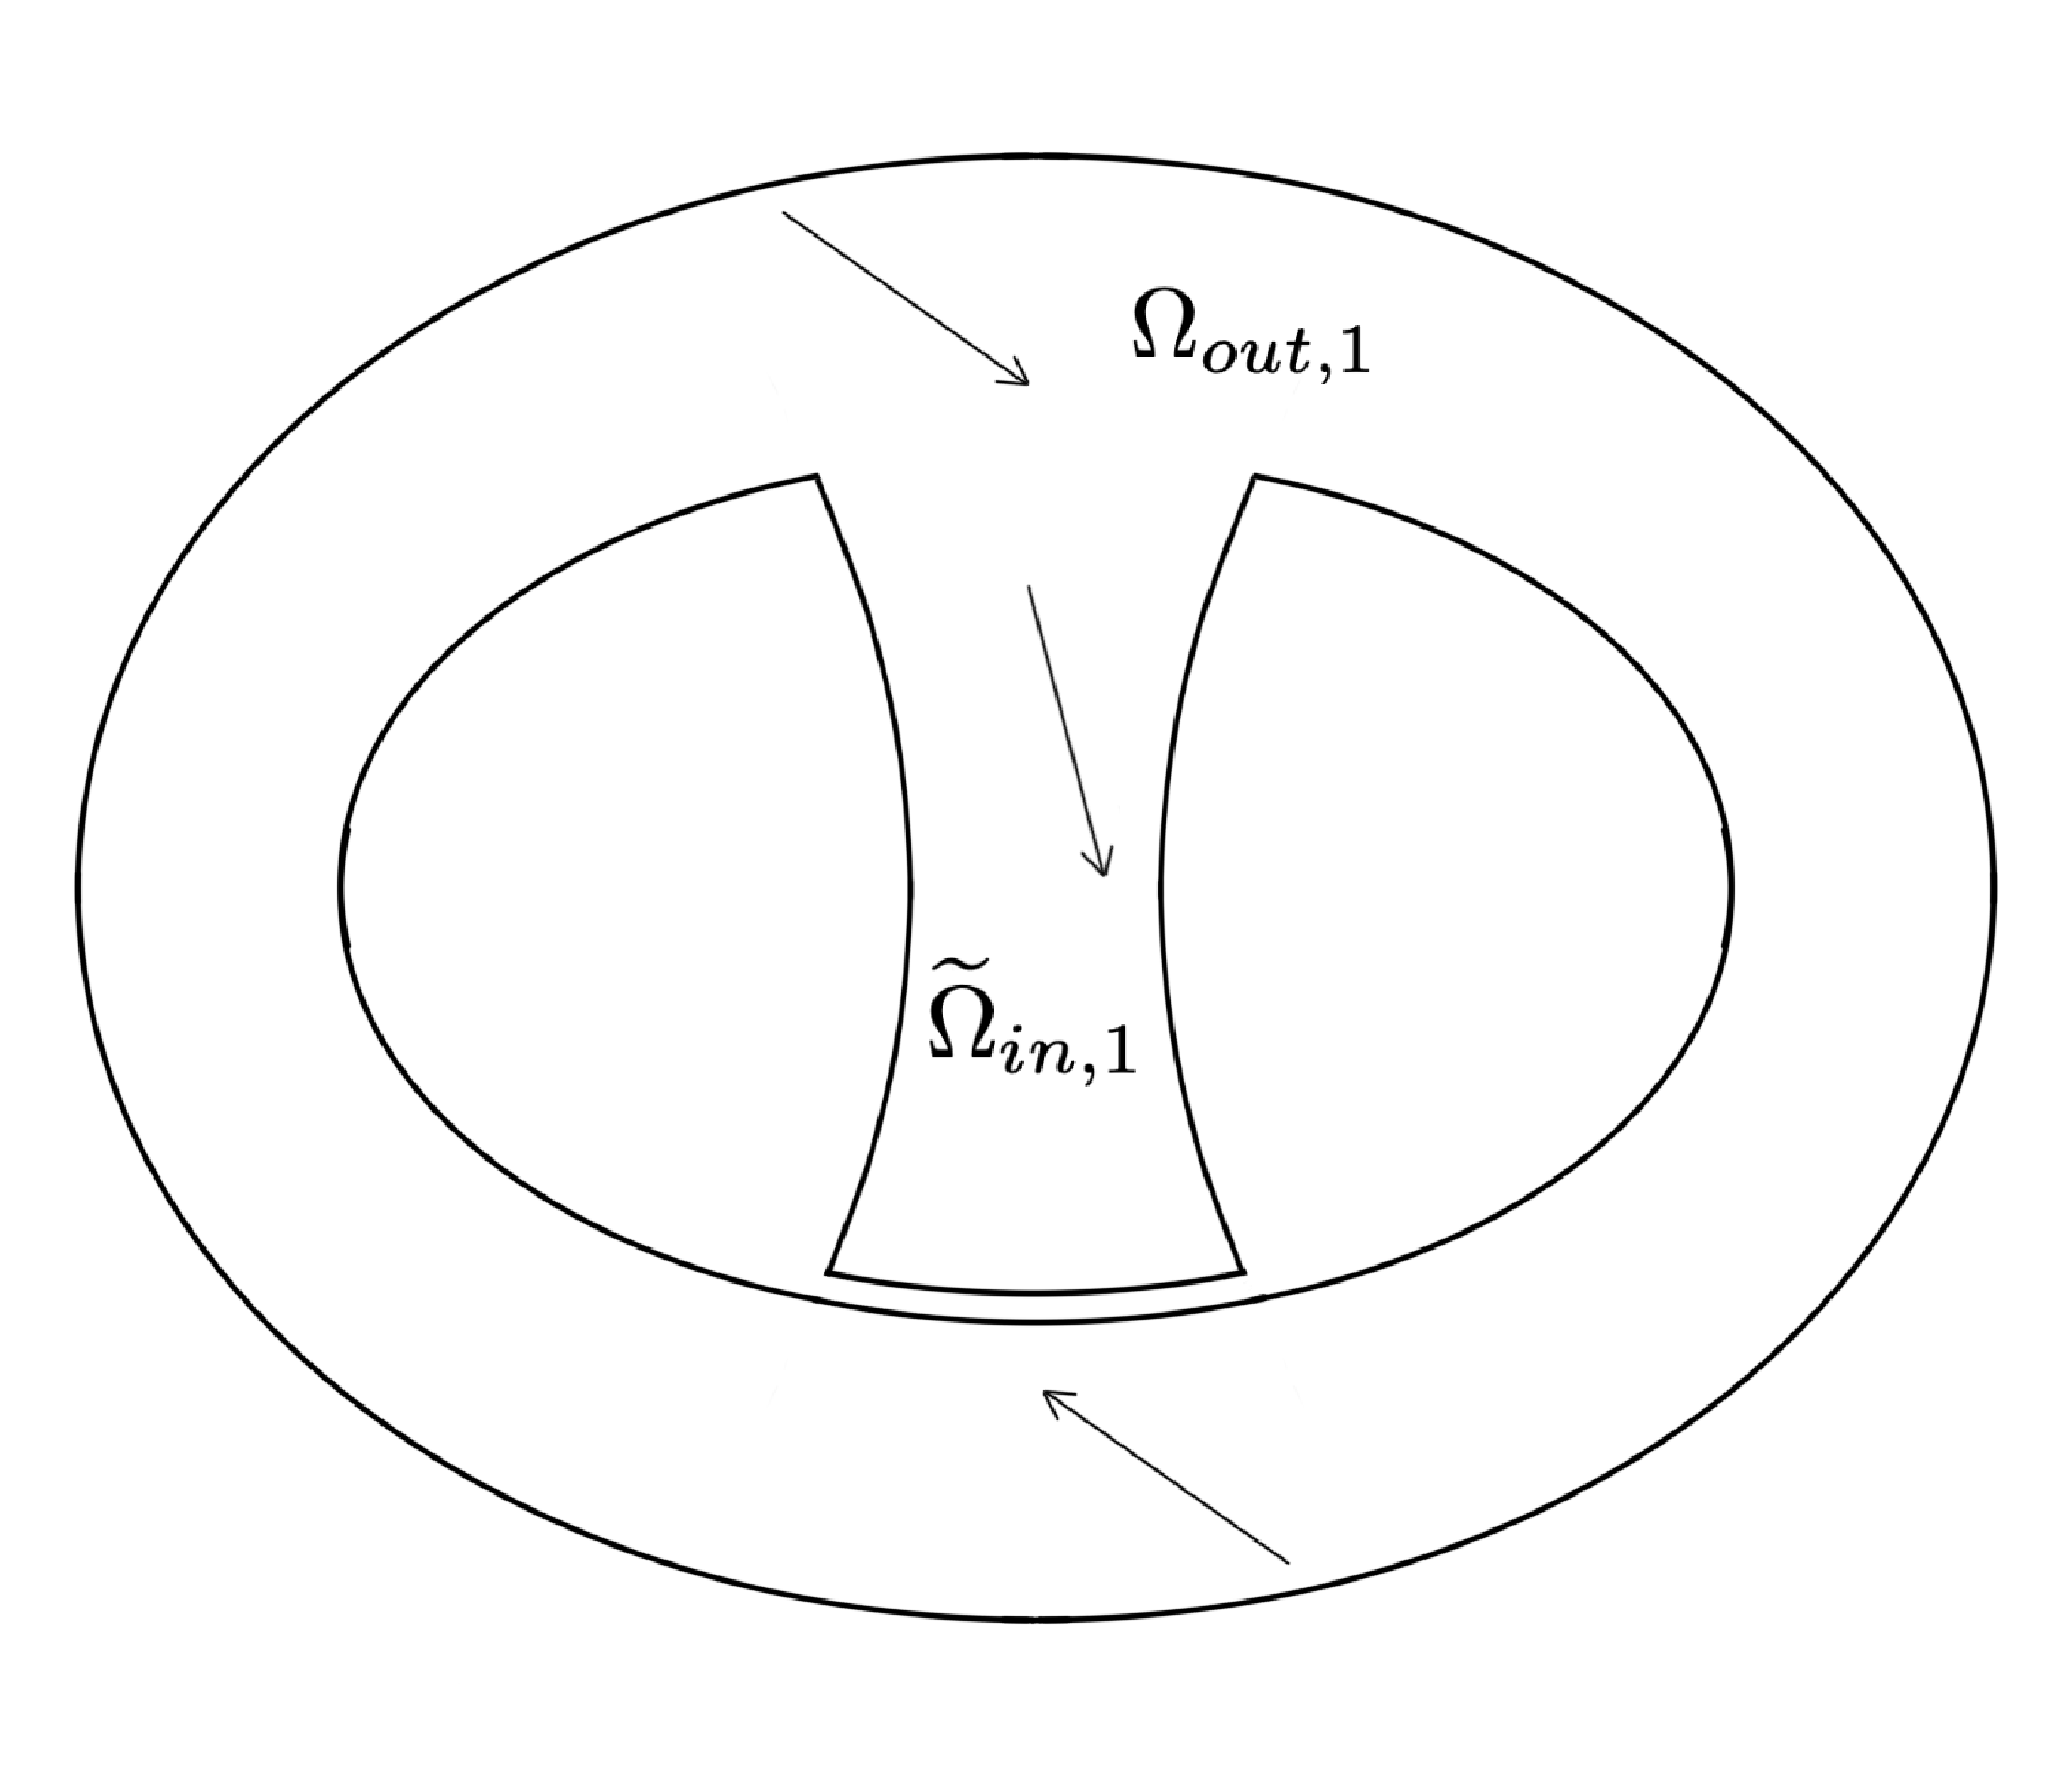
\includegraphics[width=5cm]{images/section2/ell_and_hyp2.pdf}
    \caption{Область $\widetilde{\Omega}_1$.}
    \label{fig:pt9:_ell_and_hyp_2}
\endminipage\hfill
\minipage{0.6\textwidth}
\centering
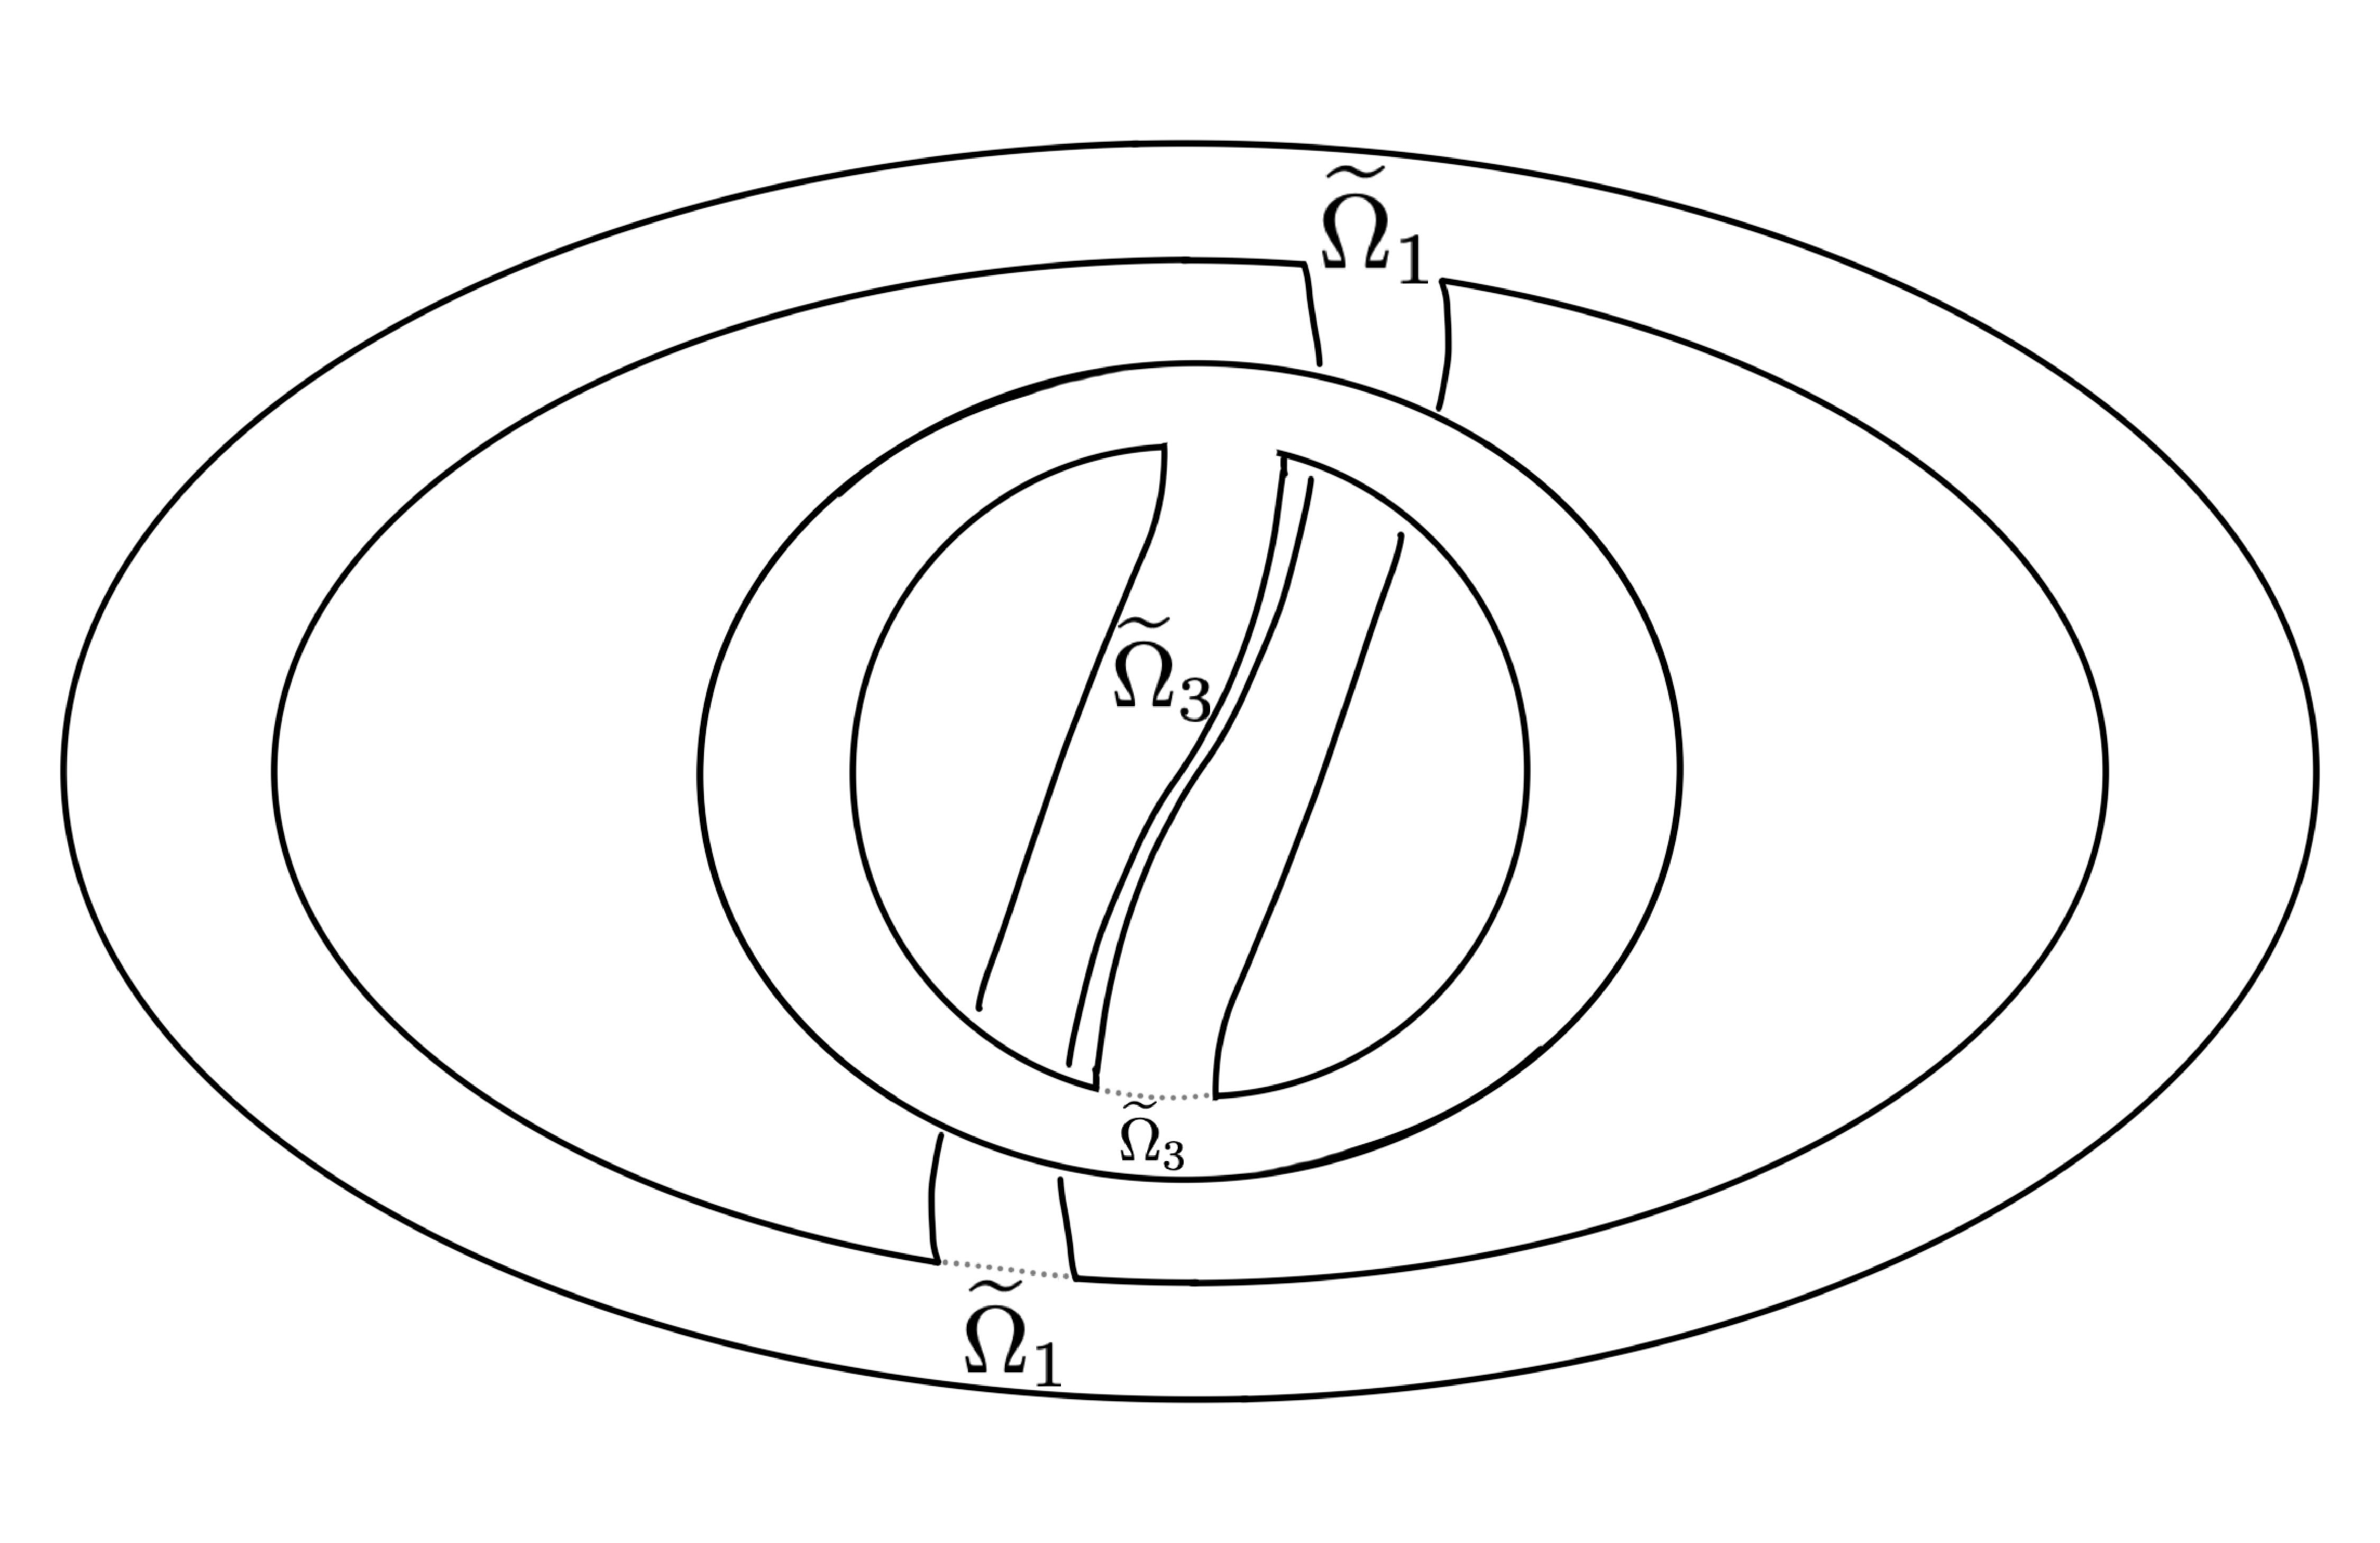
\includegraphics[width=7cm]{images/section2/ell_and_hyp2_permutations.pdf}
    \caption{Результат склейки $\widetilde{\Omega}_1$ и $\widetilde{\Omega}_3$ (одно эллиптическое кольцо уменьшено для наглядности).}
    \label{fig:pt9:_ell_and_hyp2_permutations}
\endminipage\hfill
\end{figure}

Склеим области $\widetilde{\Omega}_1$ и $\widetilde{\Omega}_3$ по эллиптическим граничным дугам, проектирующимся в нижнюю полуплоскость. Результат склейки изображен на рис. \ref{fig:pt9:_ell_and_hyp2_permutations}, пунктиром показано место склейки.  Аналогичным образом склеим области $\widetilde{\Omega}_2$ и $\widetilde{\Omega}_4$. 
Отождествляя одноименные эллиптические границы  $\widetilde{\Omega}_1 \cup \widetilde{\Omega}_3$ и $\widetilde{\Omega}_2 \cup \widetilde{\Omega}_4$, получим два соединенных лентами тора (см. рис. \ref{fig:pt9:_ell_and_hyp2_transformations}) (поверхность рода 2 с 4 дырками). Склейка областей $\widetilde{\Omega}_1$ с $\widetilde{\Omega}_2$ (аналогично $\widetilde{\Omega}
_3$ с $\widetilde{\Omega}_4$) по сегментам граничных гипербол отождествляет границы лент (склеивает края двух дырок друг с другом), что превращает их в две ручки. Таким образом, поверхность $\Xi=\const$ является сферой с пятью ручками.
\begin{figure}[!ht]
\centering
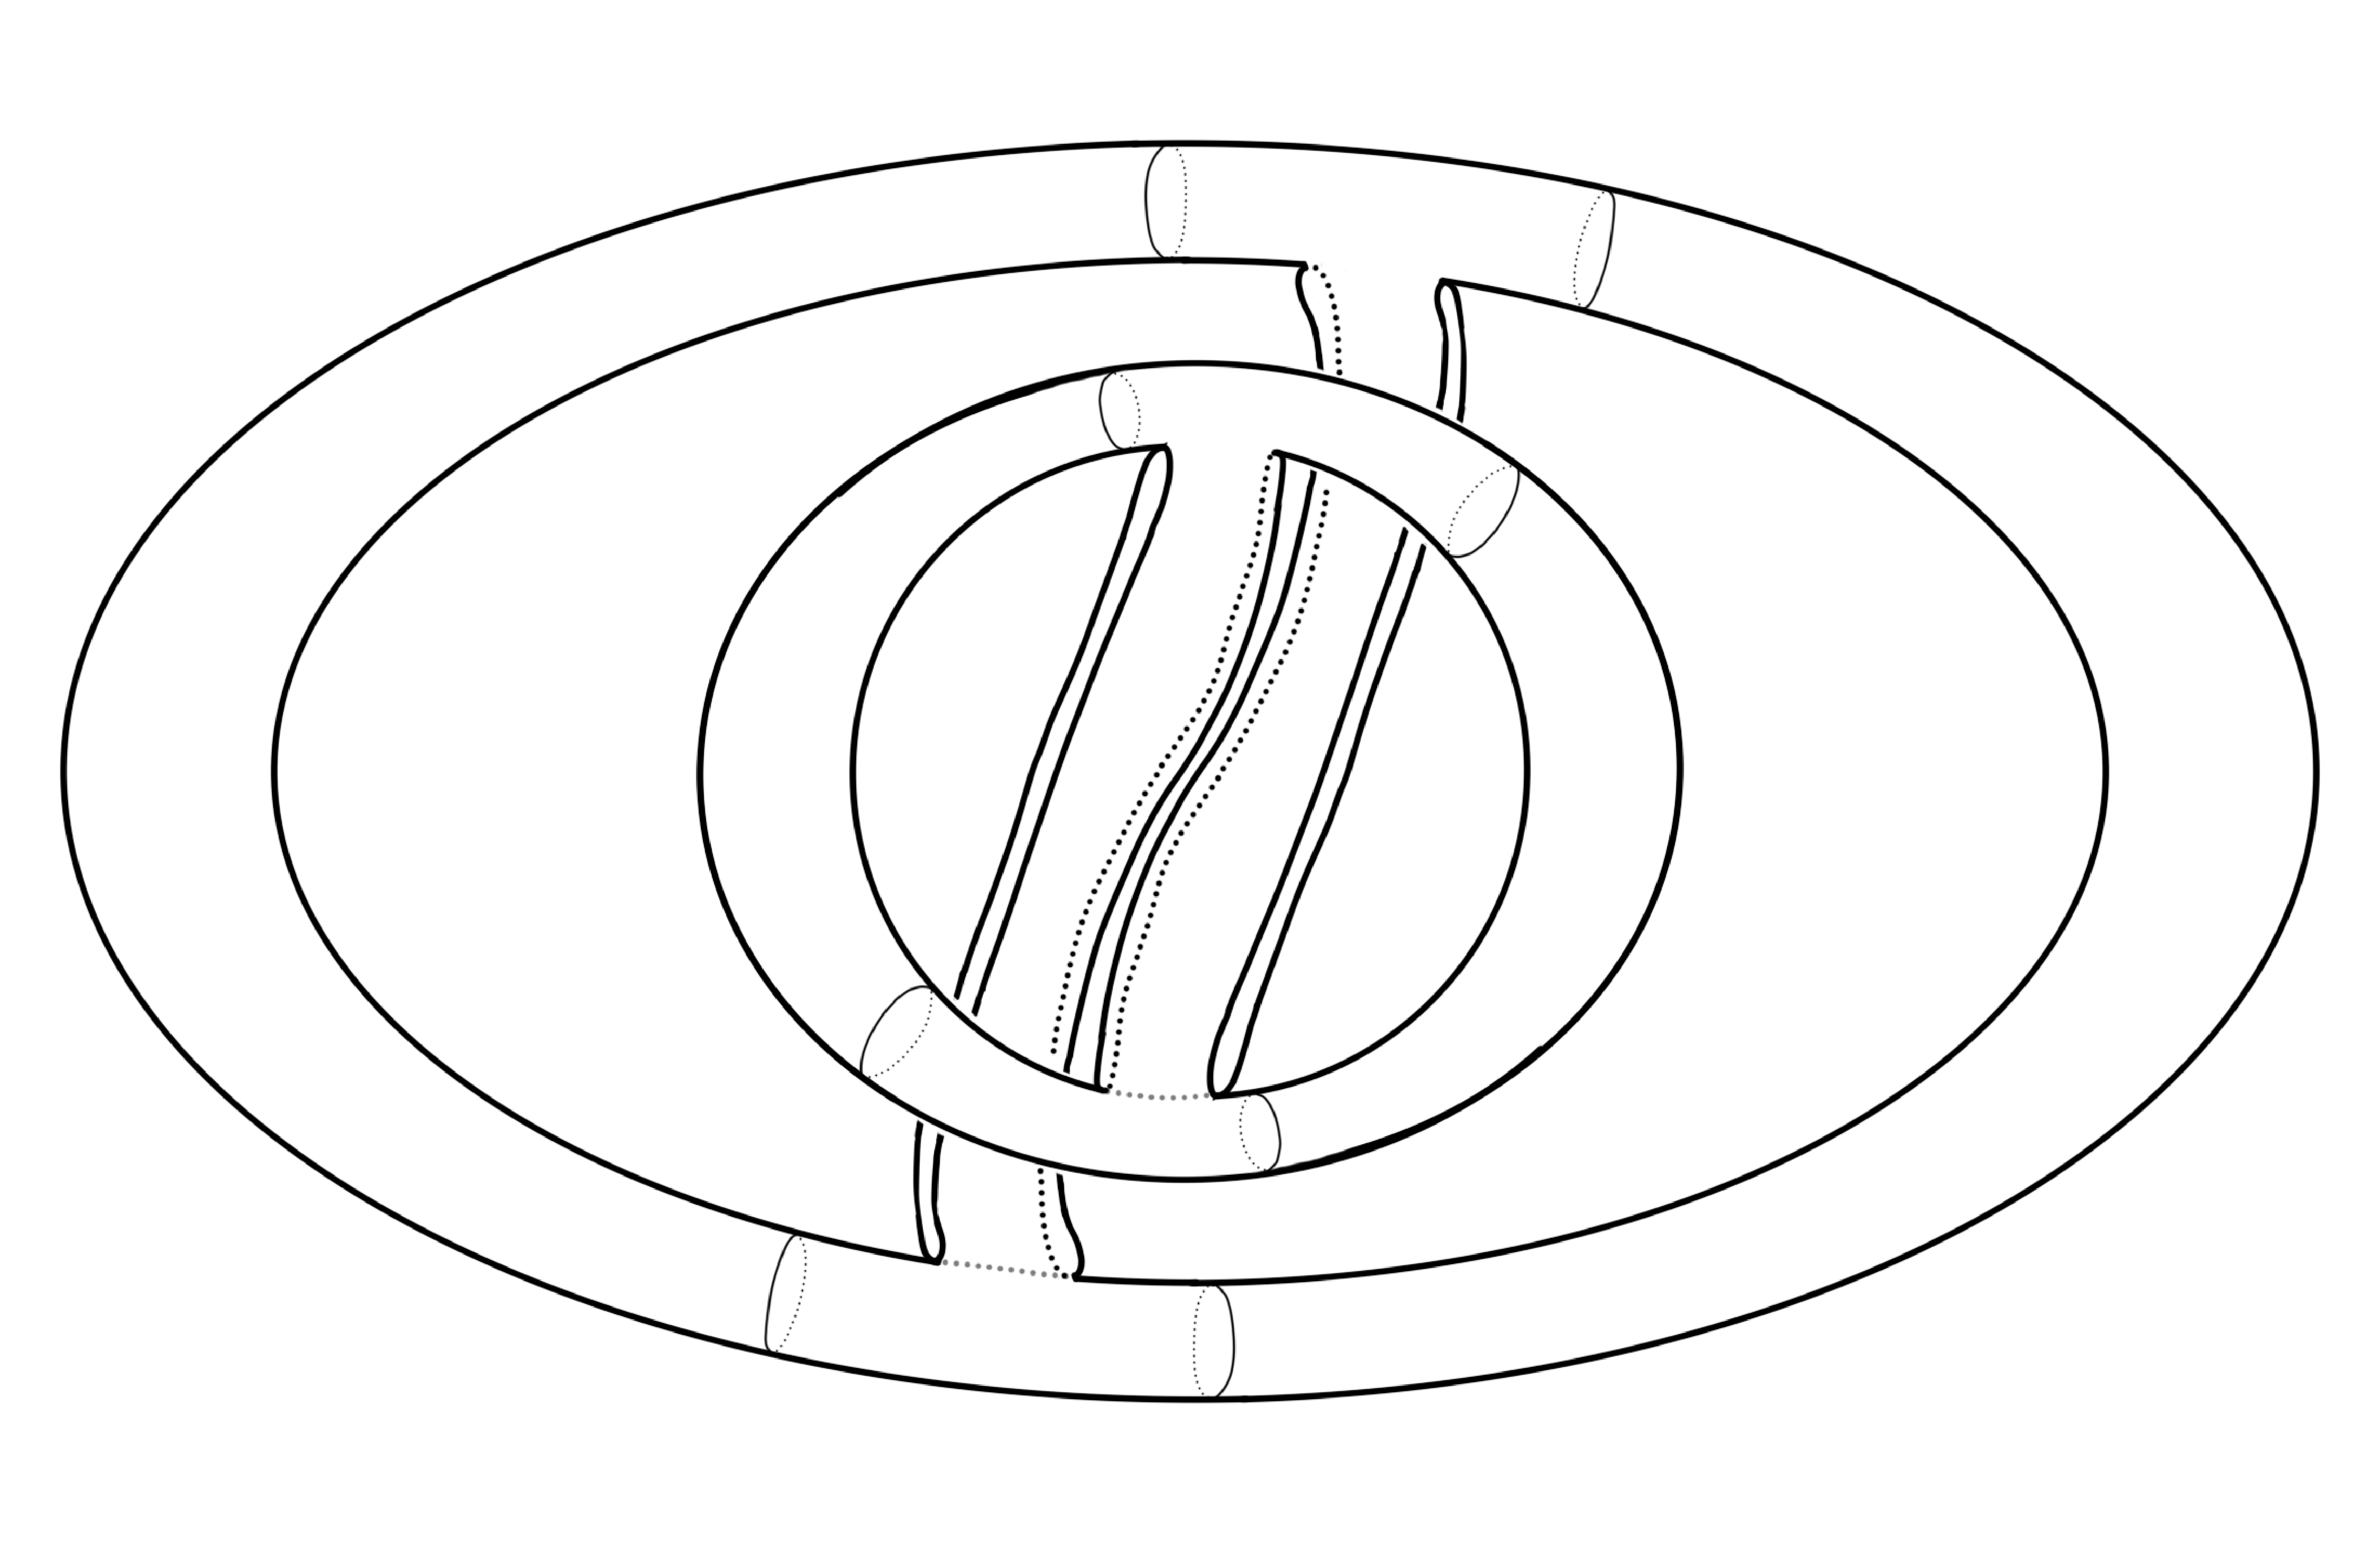
\includegraphics[scale=0.08]{images/section2/ell_and_hyp2_transformations.pdf}
    \caption{Склейка листов по эллиптическим листам --- это два тора, соединенных лентами.}
    \label{fig:pt9:_ell_and_hyp2_transformations}
\end{figure}
\end{proof}

\subsection{Поверхности уровня для нерегулярных значений интеграла $\Xi$}\label{s2.1.2} 
Теперь обратимся к перестройкам поверхностей уровня интеграла $\Xi$. 
Согласно теореме \ref{st:pt9:n1_n2_surfaces}, особые значения соответствуют точкам пересечения координатных линий $\alpha_{out}, \alpha_{in} = b^2, a^2$ с прямой \eqref{eq:L_line}, которая определяется тройкой $(\lambda_1, n_{in}, n_{out})$.
Дополним диаграмму  \ref{fig:pt9:_problemA_subdivisions}, на которой жирными линиями отмечены места, где интеграл $\Xi$ может принимать нерегулярные значения. А именно на рис. \ref{fig:pt9:_diagramPlusIrregular} мы перенумеровали различные варианты перестроек поверхностей уровня интеграла $\Xi$. 
Например, стрелка с номером 2 означает, что прямая \eqref{eq:L_line} пересекает области $D_1^5$ и $D_1^6$ и при росте значения интеграла $\Xi$ при определенном критическом значении пересекает границу $\alpha_{in} = b^2$. Эта перестройка описывается ниже в подразделе \textbf{Перестройка 2}.

\begin{figure}[!htb]
\centering
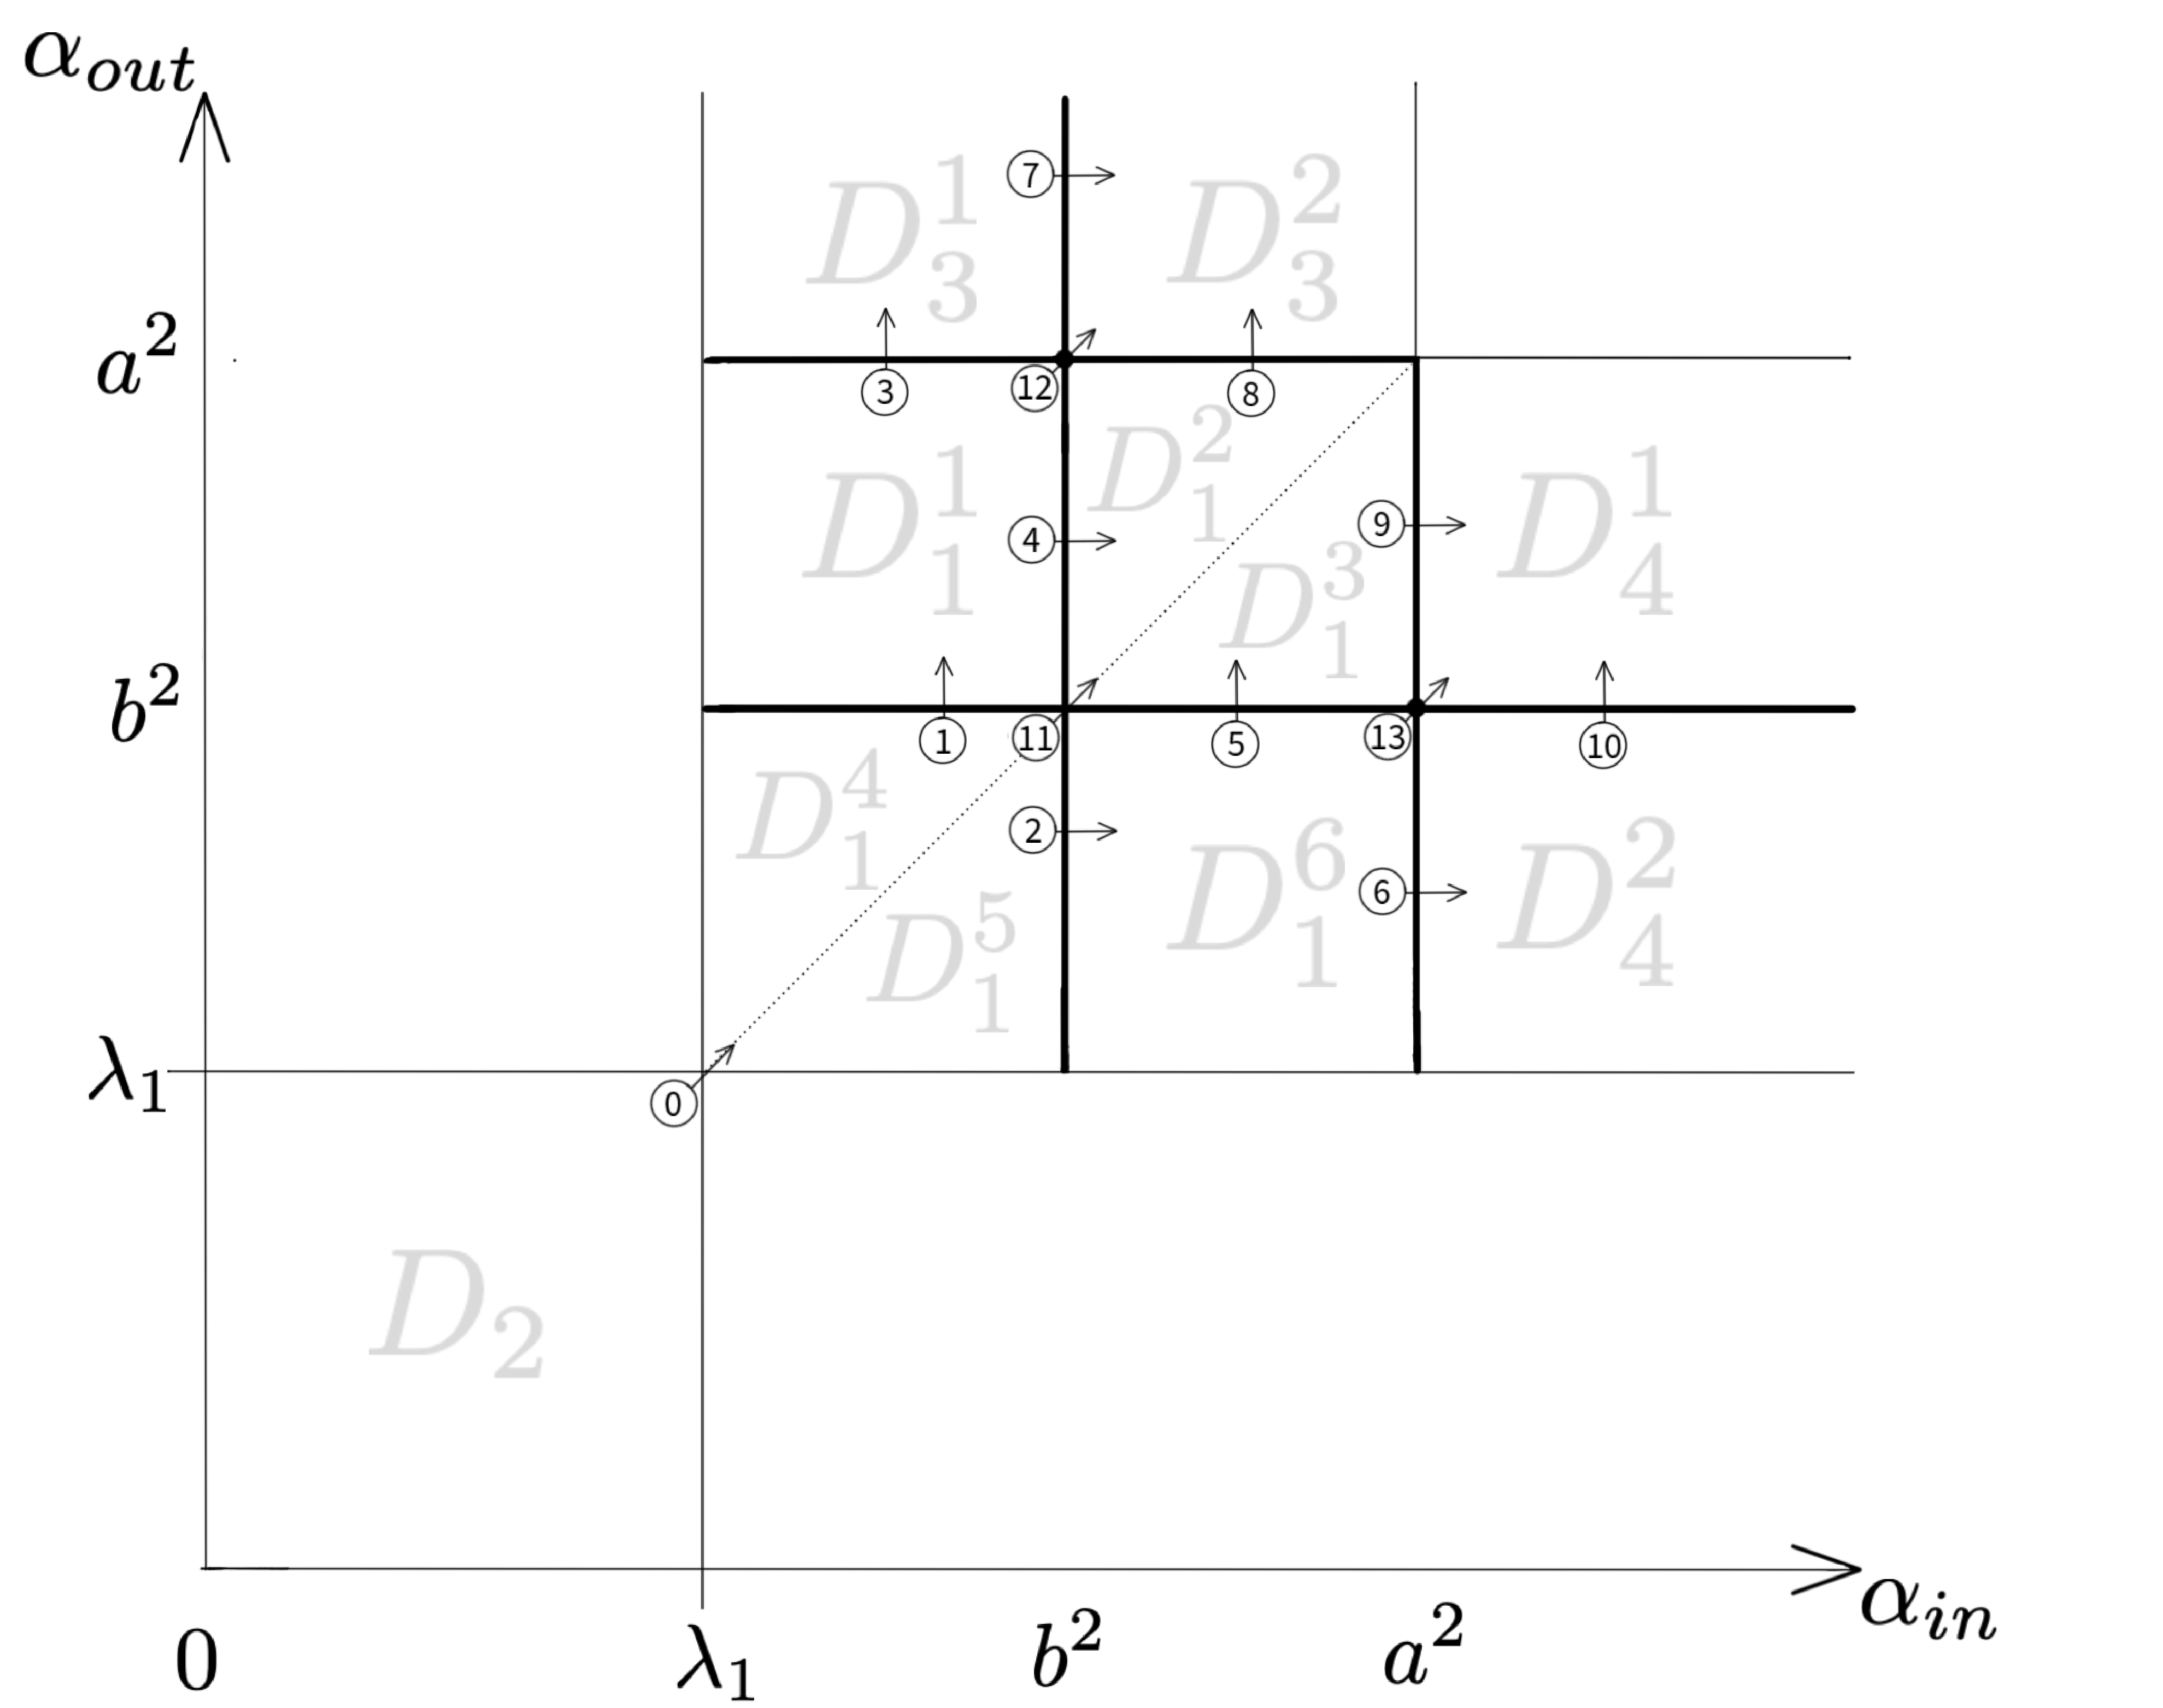
\includegraphics[width=10cm]{images/section2/diagramPlusIrregular.pdf}
    \caption{Расположение точек, соответствующих нерегулярным значениям $\Xi$.}
    \label{fig:pt9:_diagramPlusIrregular}
\end{figure}

Напомним, что прямая  \eqref{eq:L_line} проходит через точку $(\alpha_{in}, \alpha_{out}) = (\lambda_1, \lambda_1)$ и имеет коэффициент наклона $\dfrac{n_{in}^2}{n_{out}^2}$. Формула \eqref{XiToLine} устанавливает соответствие между значениями интеграла $\Xi$ и точками этой прямой. При возрастании значения интеграла $\Xi$ соответствующая точка на прямой двигается направо вверх. 

\textbf{Перестройка 0} объединяет три случая: переход из $D_2$ в область $D_1^4$, в область $D_1^5$ или на разделяющую их диагональ.
В каждом из этих трех случаев с топологической точки зрения перестройки не происходит: при проходе через особое значение поверхности уровня не меняются (2 тора). 

\textbf{Перестройка 1.} 
Сегменты траектории, находящиеся в области $\Omega_{in}$, касаются эллипса с параметром $\alpha_{in}$. 
В эллиптическом кольце $\Omega_{out}$ звенья траектории лежат на проходящих через фокусы прямых.

Положим $\widetilde{\Omega}_{in} = \Omega_{in} \setminus \Omega_{\alpha_{in}}$. 
В каждой точке $(x,y) \in \Omega_{out} \setminus \{y=0\}$ проекция $\pi$ четырехлистна. Разрежем эллиптическое кольцо вдоль горизонтальной прямой: $\Omega_{out} = \Omega_{out}^u \cup \Omega_{out}^d$, тогда проекция $(x, y, v_x, v_y) \mapsto (x,y)$ будет четырехлистна в каждой внутренней точке любой из полученных областей.
На поверхности $\Xi = \const$ выберем по 4 прообраза для верхней и нижней половины кольца. Обозначим эти прообразы $\Omega_{out, j}^u, \Omega_{out, j}^d, j=1, \ldots, 4$, где нумерацию определим согласно следующему правилу:
\begin{equation}
\begin{array}{ll}
1: & \text{ вектор } (v_x, v_y) \text{ направлен к правому фокусу }, \\
2: & \text{ вектор } (v_x, v_y) \text{ направлен к левому фокусу }, \\
3: & \text{ вектор } (v_x, v_y) \text{ направлен от правого фокуса }, \\
4: & \text{ вектор } (v_x, v_y) \text{ направлен от левого фокуса}.
\end{array}
\label{eq:foc_numeration}
\end{equation}
При этом прообразы  $\widetilde{\Omega}_{in, j}, j=1, \ldots, 4$ занумерованы в соответствии с правилом \eqref{eq:ell_numeration}.

Области $\Omega_{out, j}^u$ и $\widetilde{\Omega}_{in, j}$ для каждого $j=1, \ldots, 4$ отождествляются по общей границе в соответствии с законом преломления $(\ast)$; общая граница указанных областей проецируется в дугу эллипса $Q_{\lambda_1} \cap \{y > 0\}$. 
В симметричную ей дугу в нижней полуплоскости отображается общая для областей $\widetilde{\Omega}_{in, 1}$ и $\Omega_{out, 2}^d$ граница на поверхности $\Xi = \const$. Аналогично отождествляются области $\widetilde{\Omega}_{in, 2}$ и $\Omega_{out, 1}^d$, $\widetilde{\Omega}_{in, 3}$ и $\Omega_{out, 4}^d$, а также $\widetilde{\Omega}_{in, 4}$ и $\Omega_{out, 3}^d$.

Отметим, что горизонтальная прямая пересекается с кольцом $\Omega_{out}$ по двум отрезкам $I_1$ и $I_2$. На каждый из них проецируются общие границы для четверок областей: $\Omega_{out, 1}^u, \Omega_{out, 1}^d, \Omega_{out, 2}^u, \Omega_{out, 2}^d$. Аналогично для областей $\Omega_{out, 3}^u, \Omega_{out, 3}^d$, $ \Omega_{out, 4}^u, \Omega_{out, 4}^d$.

Определим области $\widetilde{\Omega}_1 = \Omega_{out, 1}^u \cup \widetilde{\Omega}_{in, 1} \cup \Omega_{out, 2}^d$, $\widetilde{\Omega}_2 = \Omega_{out, 2}^u \cup \widetilde{\Omega}_{in, 2} \cup \Omega_{out, 1}^d$, аналогично определим области $\widetilde{\Omega}_3 = \Omega_{out, 3}^u \cup \widetilde{\Omega}_{in, 3} \cup \Omega_{out, 4}^d$ и $\widetilde{\Omega}_4 = \Omega_{out, 4}^u \cup \widetilde{\Omega}_{in, 4} \cup \Omega_{out, 3}^d$. Пример области $\widetilde{\Omega}_1$ см. рис. \ref{fig:pt9:_domain_atom_ell_foc},  жирным пунктиром  изображен отрезок, проецирующийся в  $I_1$, а жирным сплошным --- проецирующийся в $I_2$.

\begin{figure}[!htb]
\minipage{0.43\textwidth}
\centering
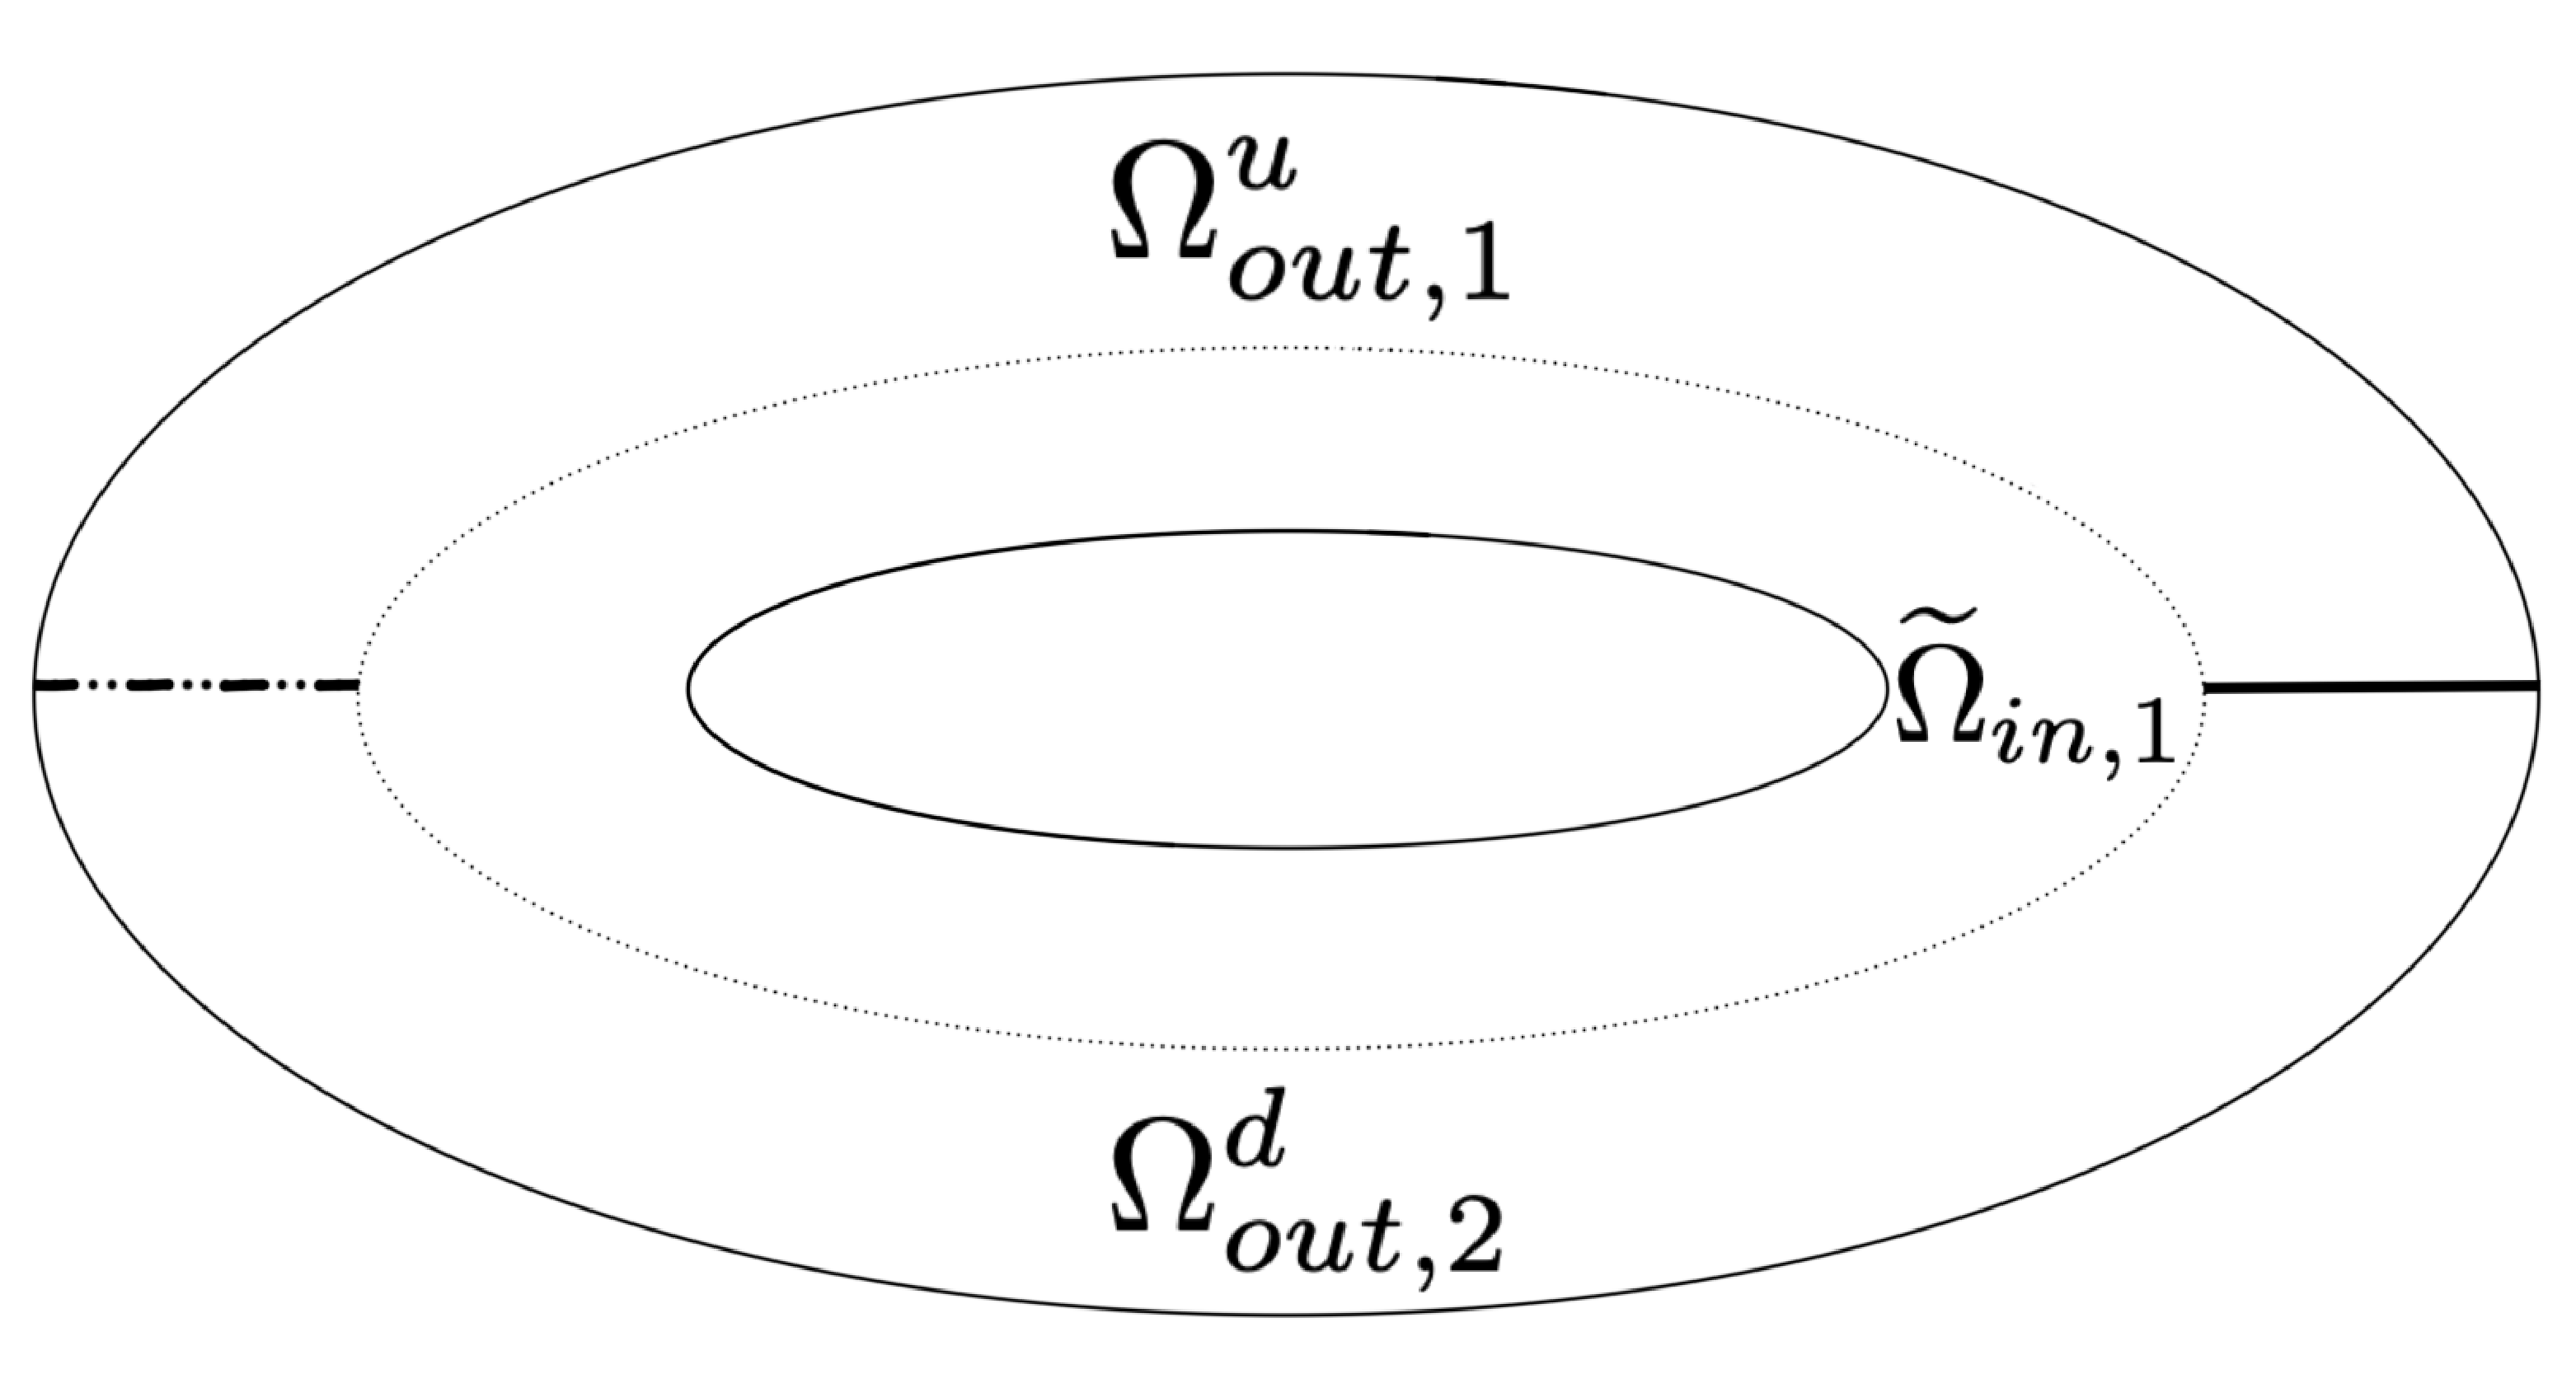
\includegraphics[scale=0.125]{images/section2/atoms/domain_atom_ell_foc.pdf}
    \caption{Пример области $\widetilde{\Omega}_1$ для перестройки 1.}
    \label{fig:pt9:_domain_atom_ell_foc}
\endminipage\hfill
\minipage{0.42\textwidth}
\centering
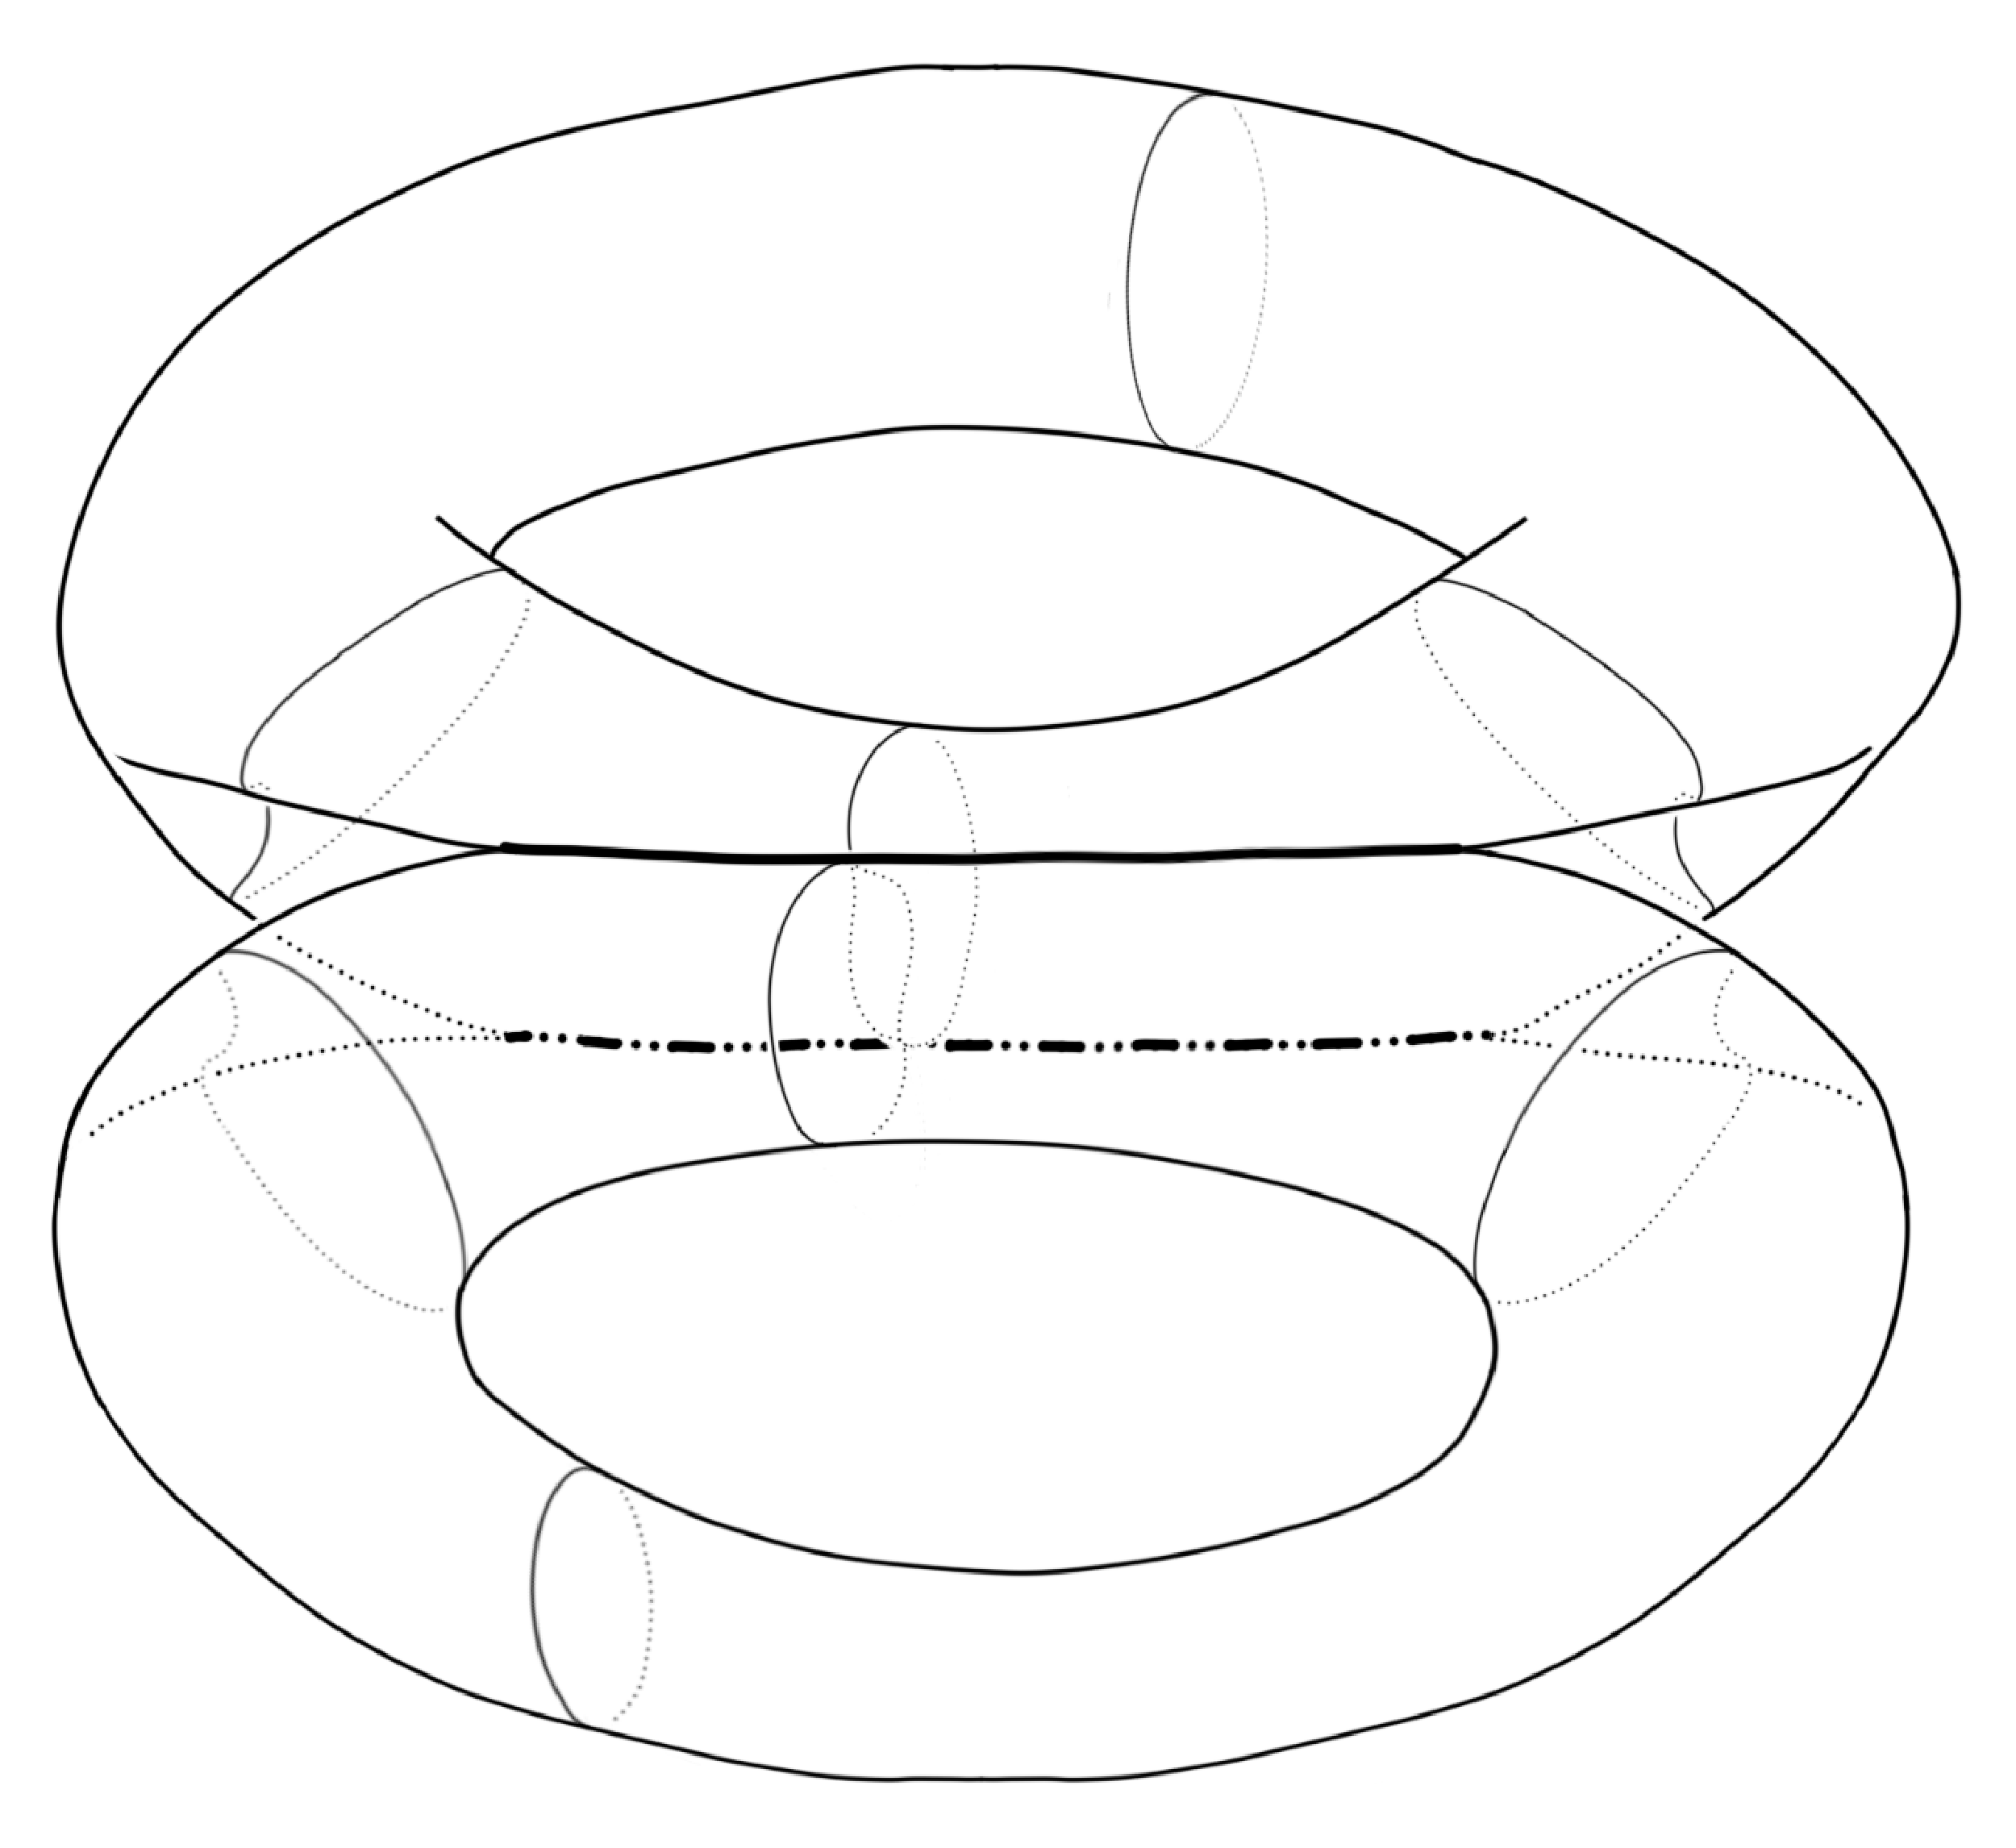
\includegraphics[scale=0.125]{images/section2/atoms/atom1_result.pdf}
    \caption{Поверхность уровня $\Xi=\const$ для перестройки 1.}
    \label{fig:pt9:_atom1_result}
\endminipage\hfill
\end{figure}


Склеим области $\widetilde{\Omega}_1$ и $\widetilde{\Omega}_4$ по одноименным эллиптическим границам, получим один тор. Аналогично для областей $\widetilde{\Omega}_2$ и $\widetilde{\Omega}_3$.

При этом на торе $\widetilde{\Omega}_1 \cup \widetilde{\Omega}_4$ в одной конечной точке отождествляются два прообраза пунктирного  отрезка $I_1$, аналогично для сплошного отрезка $I_2$. На  торе $\widetilde{\Omega}_2 \cup \widetilde{\Omega}_3$ также присутствуют кривые, двулистно накрывающие отрезки $I_1$ и  $I_2$.
На рис. \ref{fig:pt9:_atom1_result} кривые изображены жирным и пунктиром.
Остается отождествить два тора по этим кривым, тогда поверхность уровня $\Xi = \const$ представляет собой склейку двух торов по двум конечным отрезкам (см. рис. \ref{fig:pt9:_atom1_result}). 


\textbf{Перестройка 2.} 
Сегменты бильярдной траектории в области $\Omega_{in}$ лежат на прямых, проходящих через фокусы, а продолжения звеньев траектории в кольце $\Omega_{out}$ касаются эллипса с параметром $\alpha_{out}$. 

Проекция поверхности $\Xi = \const$ заметает всю область $\Omega$. При этом каждой внутренней точке $\Omega_{out} \cup (\Omega_{in} \setminus \{y=0\})$ соответствует четыре точки на поверхности.
Разрежем область $\Omega$ по горизонтальной прямой и представим  ее в виде объединения $\Omega_{out}^u \cup \Omega_{in}^u \cup \Omega_{in}^d \cup \Omega_{out}^d$. 
Каждой из указанных областей соответствует по четыре области на поверхности $\Xi = \const$, обозначим их $\Omega_{out, j}^u , \Omega_{in, j}^u , \Omega_{in, j}^d , \Omega_{out, j}^d, j=1, \ldots, 4$. 
При этом для прообразов $\Omega_{out, j}^u$ и $\Omega_{out, j}^d$ используем нумерацию в соответствии с правилом \eqref{eq:ell_numeration}. 
Прообразы $\Omega_{in, j}^u$ и $\Omega_{in, j}^d$ пронумерованы как в правиле \eqref{eq:foc_numeration}.

Заметим, что на поверхности $\Xi = \const$ области $\Omega_{out, j}^u$ и $\Omega_{in, j}^u$ отождествляются по общей границе, которая проектируется в дугу эллипса $Q_{\lambda_1} \cap \{ y > 0\}$, где $j=1, \ldots,4$. Обозначим $\Omega_j^u = \Omega_{out, j}^u \cup \Omega_{in, j}^u, j=1, \ldots, 4$.

В симметричную дугу в нижней полуплоскости проектируется общий сегмент границ областей $\Omega_{in, 1}^d$ и $\Omega_{out, 3}^d$, на котором эти области отождествляются. 
%Обозначим результат их склейки как $\Omega_3^d$. 
%Аналогично определим $\Omega_1^d = \Omega_{in, 2}^d \cup \Omega_{out, 1}^d$, а также $\Omega_2^d = \Omega_{in, 1}^d \cup \Omega_{out, 2}^d$ и $\Omega_4^d = \Omega_{in, 3}^d \cup \Omega_{out, 4}^d$.
Аналогично  отождествляются $\Omega_{in, 2}^d$ c $\Omega_{out, 1}^d$, а также $\Omega_{in, 1}^d$ c $\Omega_{out, 2}^d$ и $\Omega_{in, 3}^d$ с $ \Omega_{out, 4}^d$.

На горизонтальной оси можно выделить пять сегментов: два из них попадают в $\Omega_{out}$ и три в $\Omega_{in}$, один из которых соединяет фокусы.
В отрезок между фокусов проектируется общая граница для четырех областей $\Omega_1^u, \Omega_4^u, \Omega_{in, 1}^d$ и $\Omega_{in, 4}^d$.
Аналогично общая граница областей $\Omega_2^u, \Omega_3^u, \Omega_{in, 2}^d$ и $\Omega_{in, 3}^d$ проектируется на этот же отрезок.

Определим области 
\begin{equation}
\begin{array}{cc}
\widetilde{\Omega}_1 = \Omega_1^u \cup \Omega_{in, 4}^d \cup \Omega_{out, 3}^d, &
\widetilde{\Omega}_2 = \Omega_2^u \cup \Omega_{in, 3}^d \cup \Omega_{out, 4}^d, \\
\widetilde{\Omega}_3 = \Omega_3^u \cup \Omega_{in, 2}^d \cup \Omega_{out, 1}^d, &
\widetilde{\Omega}_4 = \Omega_4^u \cup \Omega_{in, 1}^d \cup \Omega_{out, 2}^d. 
\end{array}
\label{eq:case2Omegas}
\end{equation}
Пример области $\widetilde{\Omega}_1$ изображен на рис. \ref{fig:pt9:_domain_atom_foc_ell}.
 \begin{figure}[!htb]
\centering
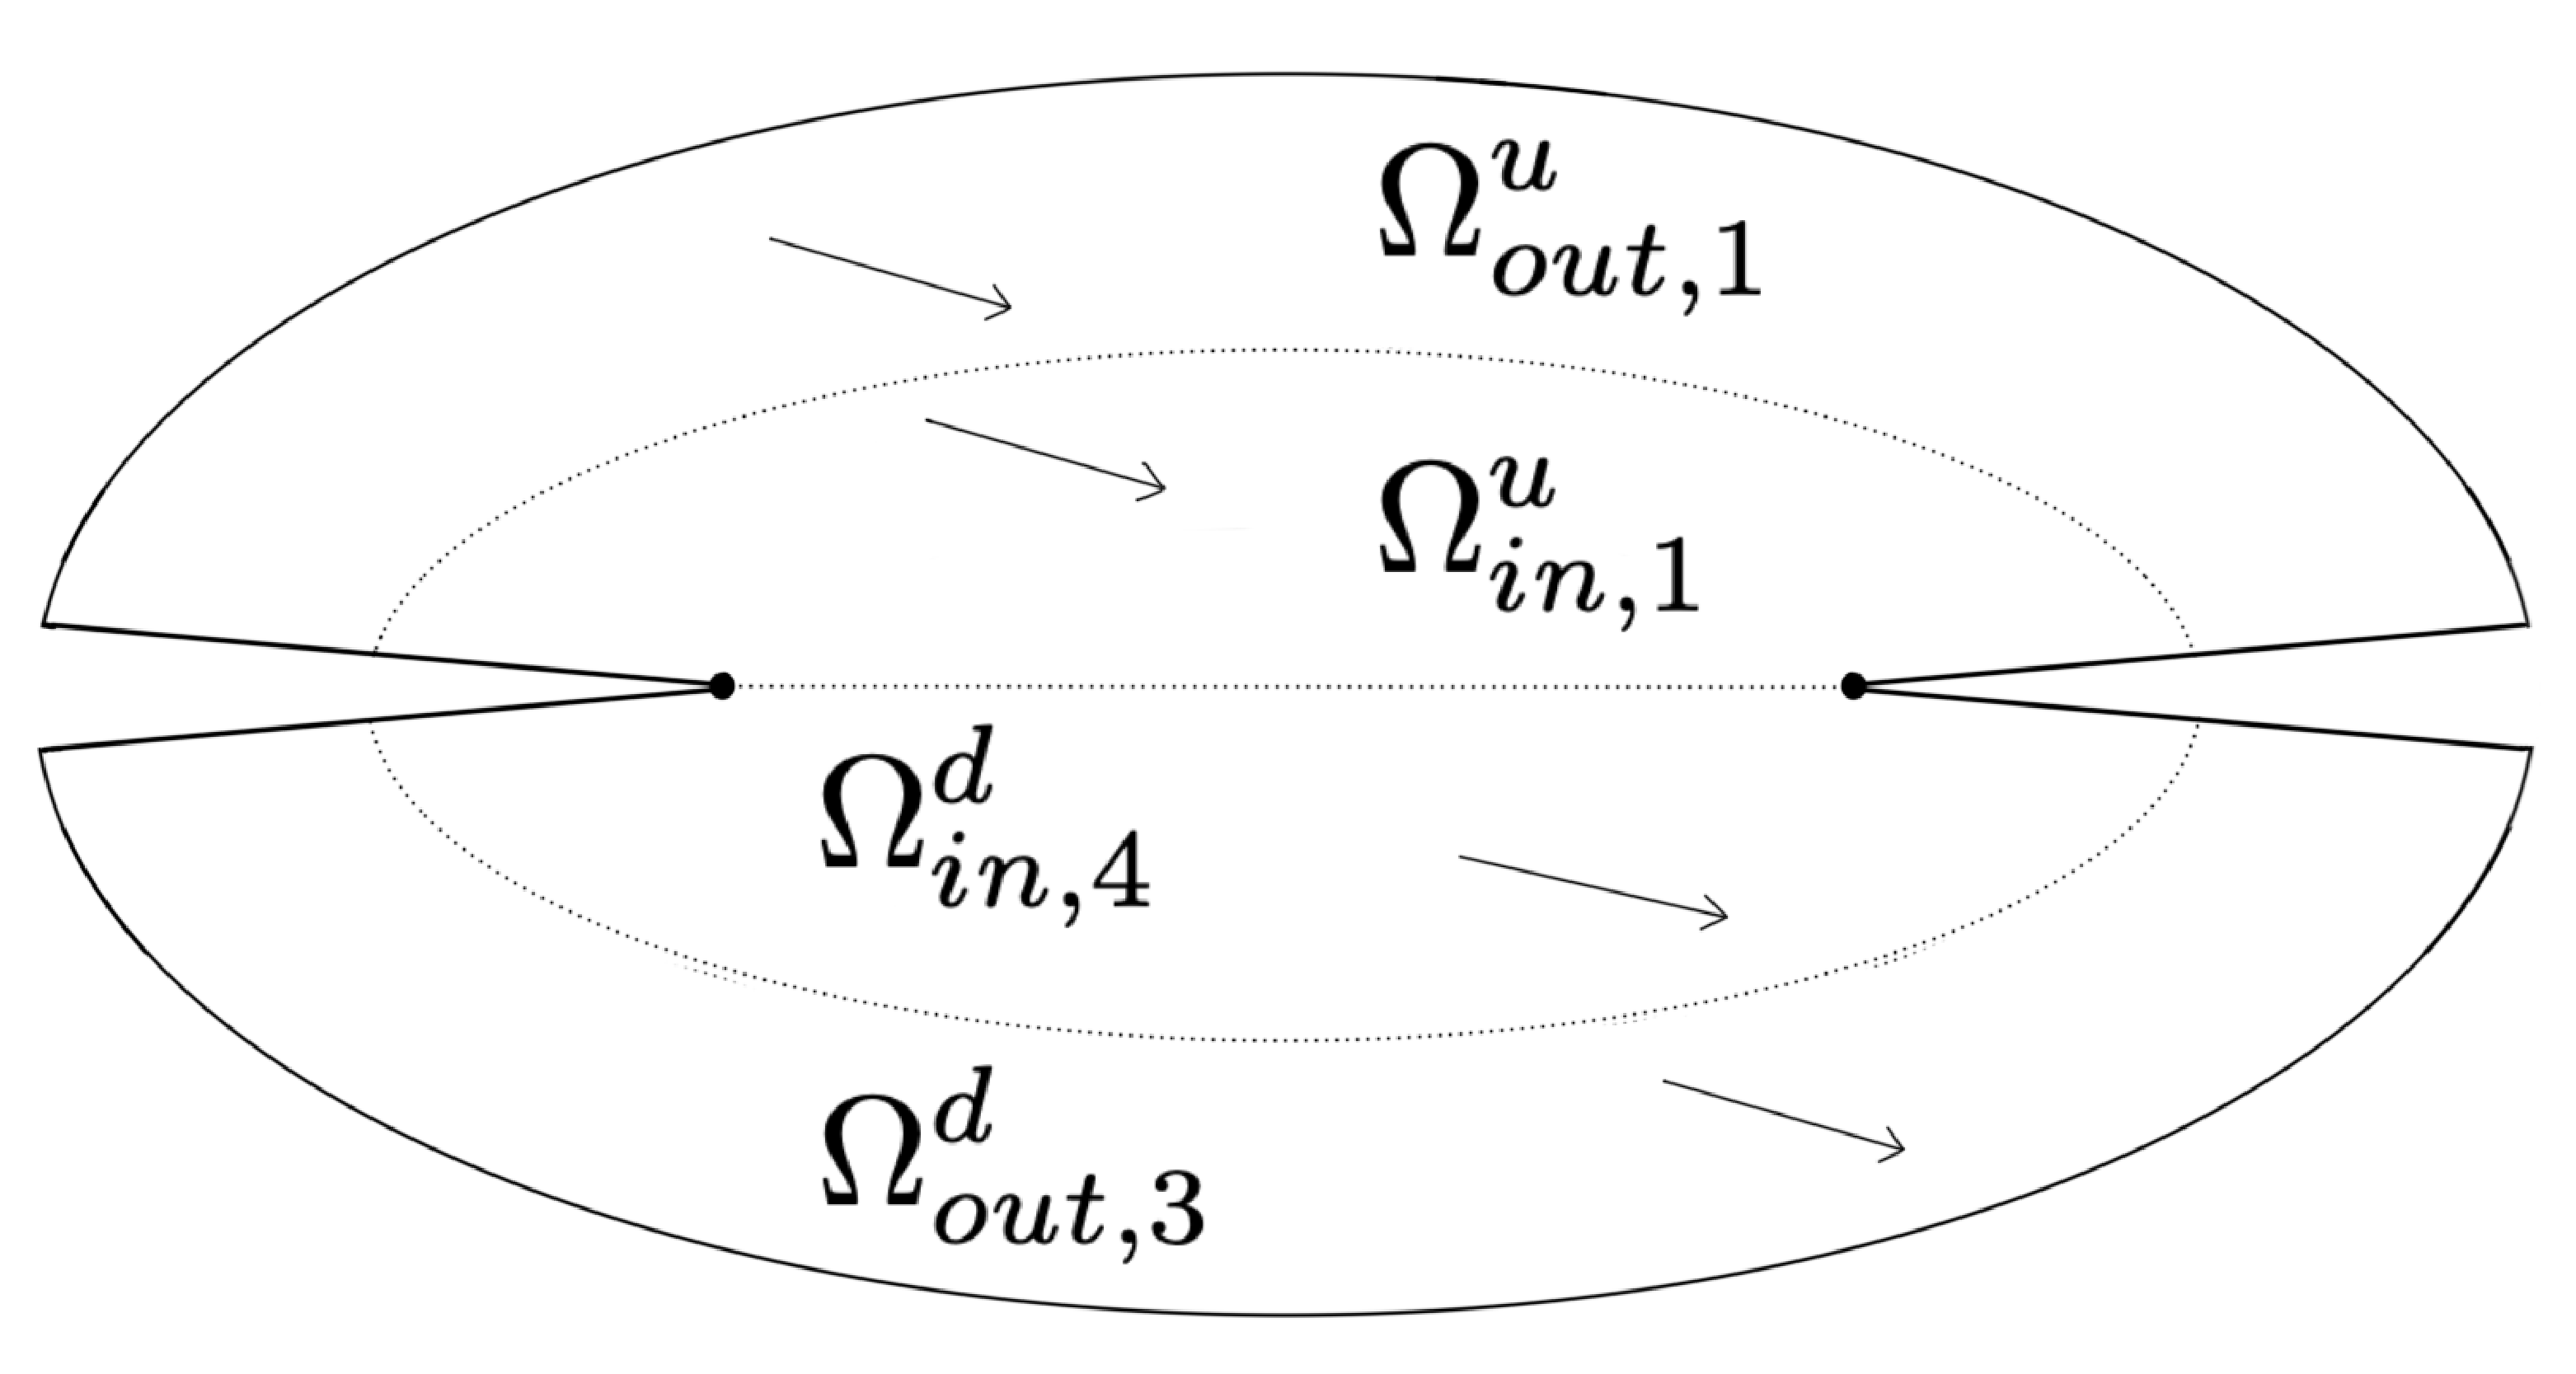
\includegraphics[scale=0.125]{images/section2/atoms/domain_atom_foc_ell.pdf}
    \caption{Пример области $\widetilde{\Omega}_1$ для перестройки 2.}
    \label{fig:pt9:_domain_atom_foc_ell}
\end{figure}
 
Склеим области $\widetilde{\Omega}_1$ и $\widetilde{\Omega}_4$ по граничным эллиптическим дугам, а также по прообразу соединяющего фокусы отрезка на $\Xi = \const$. Аналогично для областей $\widetilde{\Omega}_2$ и $\widetilde{\Omega}_3$. Получим два цилиндра; поперечное сечение каждого даст восьмерку. 

Рассмотрим прообраз на $\Xi = \const$ горизонтального отрезка, левый конец которого находится в правом фокусе, а правый --- в правой вершине $Q_{\lambda_1}$.
В этот сегмент прямой, в силу изложенных в \cite[\S 4]{Fok15} соображений, проектируется общая граница для областей $\Omega_{in, 1}^u$ и $\Omega_{in, 2}^d$. Аналогично для пар областей $\Omega_{in, 2}^u$ и $\Omega_{in, 1}^d$, $\Omega_{in, 3}^u$ и $\Omega_{in, 4}^d$ и для пары $\Omega_{in, 4}^u$ и $\Omega_{in, 3}^d$. 
То есть на поверхности $\Xi = \const$ (см. \eqref{eq:case2Omegas}) \textit{верхняя} граница области $\widetilde{\Omega}_1$ отождествляется с \textit{нижней} границей области $\widetilde{\Omega}_3$ и наоборот. Аналогично для двух других областей: \textit{верхняя} граница $\widetilde{\Omega}_2$ --- с \textit{нижней} границей области $\widetilde{\Omega}_4$ и наоборот. 
Из аналогичных соображений следуют такие же склейки на прообразе симметричного отрезка, соединяющем левую вершину эллипса $Q_{\lambda_1}$ и левый фокус.

Рассмотрим отрезки $\Omega_{out} \cap \{y=0\}$. 
На каждый из них проектируются общие границы областей $\Omega_{out, j}^u$ и $\Omega_{out, j}^d$ для $j=1, \ldots, 4$. 
То есть, по прообразу каждого из отрезков отождествляются листы (см. \eqref{eq:case2Omegas}) $\widetilde{\Omega}_1$ с $\widetilde{\Omega}_3$, а также $\widetilde{\Omega}_2$ с  $\widetilde{\Omega}_4$.
% Поскольку склейки отрезков идентичны тем, что были получены в предыдущем абзаце, будем считать их одной склейкой.

Склеим листы $\widetilde{\Omega}_1$ с $\widetilde{\Omega}_4$ по трем общим дугам и получим два соединенных вдоль общей горизонтальной прямой цилиндра (или, что то же самое, цилиндр с восьмеркой в сечении). Аналогично склеим листы $\widetilde{\Omega}_2$ и $\widetilde{\Omega}_3$.
При этом две дуги, ограничивающие левую окружность верхнего цилиндра $\widetilde{\Omega}_1 \cup \widetilde{\Omega}_4$, проектируются в отрезок горизонтальной прямой, соединяющий левую вершину граничного эллипса с левым фокусом. В этот же отрезок проецируются дуги, ограничивающие левую окружность правого цилиндра  $\widetilde{\Omega}_1 \cup \widetilde{\Omega}_4$. Аналогично для $\widetilde{\Omega}_2$ и $\widetilde{\Omega}_3$. То же самое справедливо для дуг, ограничивающих правые окружности цилиндров, только проецируются они на симметричный горизонтальный отрезок от правого фокуса к правой вершине граничного эллипса.
Остается склеить цилиндры между собой: левая окружность \textit{верхнего} цилиндра $\widetilde{\Omega}_1 \cup \widetilde{\Omega}_4$ отождествляется с левой окружностью \textit{нижнего} цилиндра $\widetilde{\Omega}_2 \cup \widetilde{\Omega}_3$, а левая окружность \textit{нижнего} цилиндра $\widetilde{\Omega}_1 \cup \widetilde{\Omega}_4$ --- с левой окружностью \textit{верхнего} цилиндра $\widetilde{\Omega}_2 \cup \widetilde{\Omega}_3$. 
Аналогичные склейки возникают на правых окружностях цилиндров. 

Таким образом, поверхность $\Xi = \const$ представляет собой тор с восьмеркой в продольном сечении, см. рис. \ref{fig:pt9:_foc_ell_atom}.
\begin{figure}[!htb]
\centering
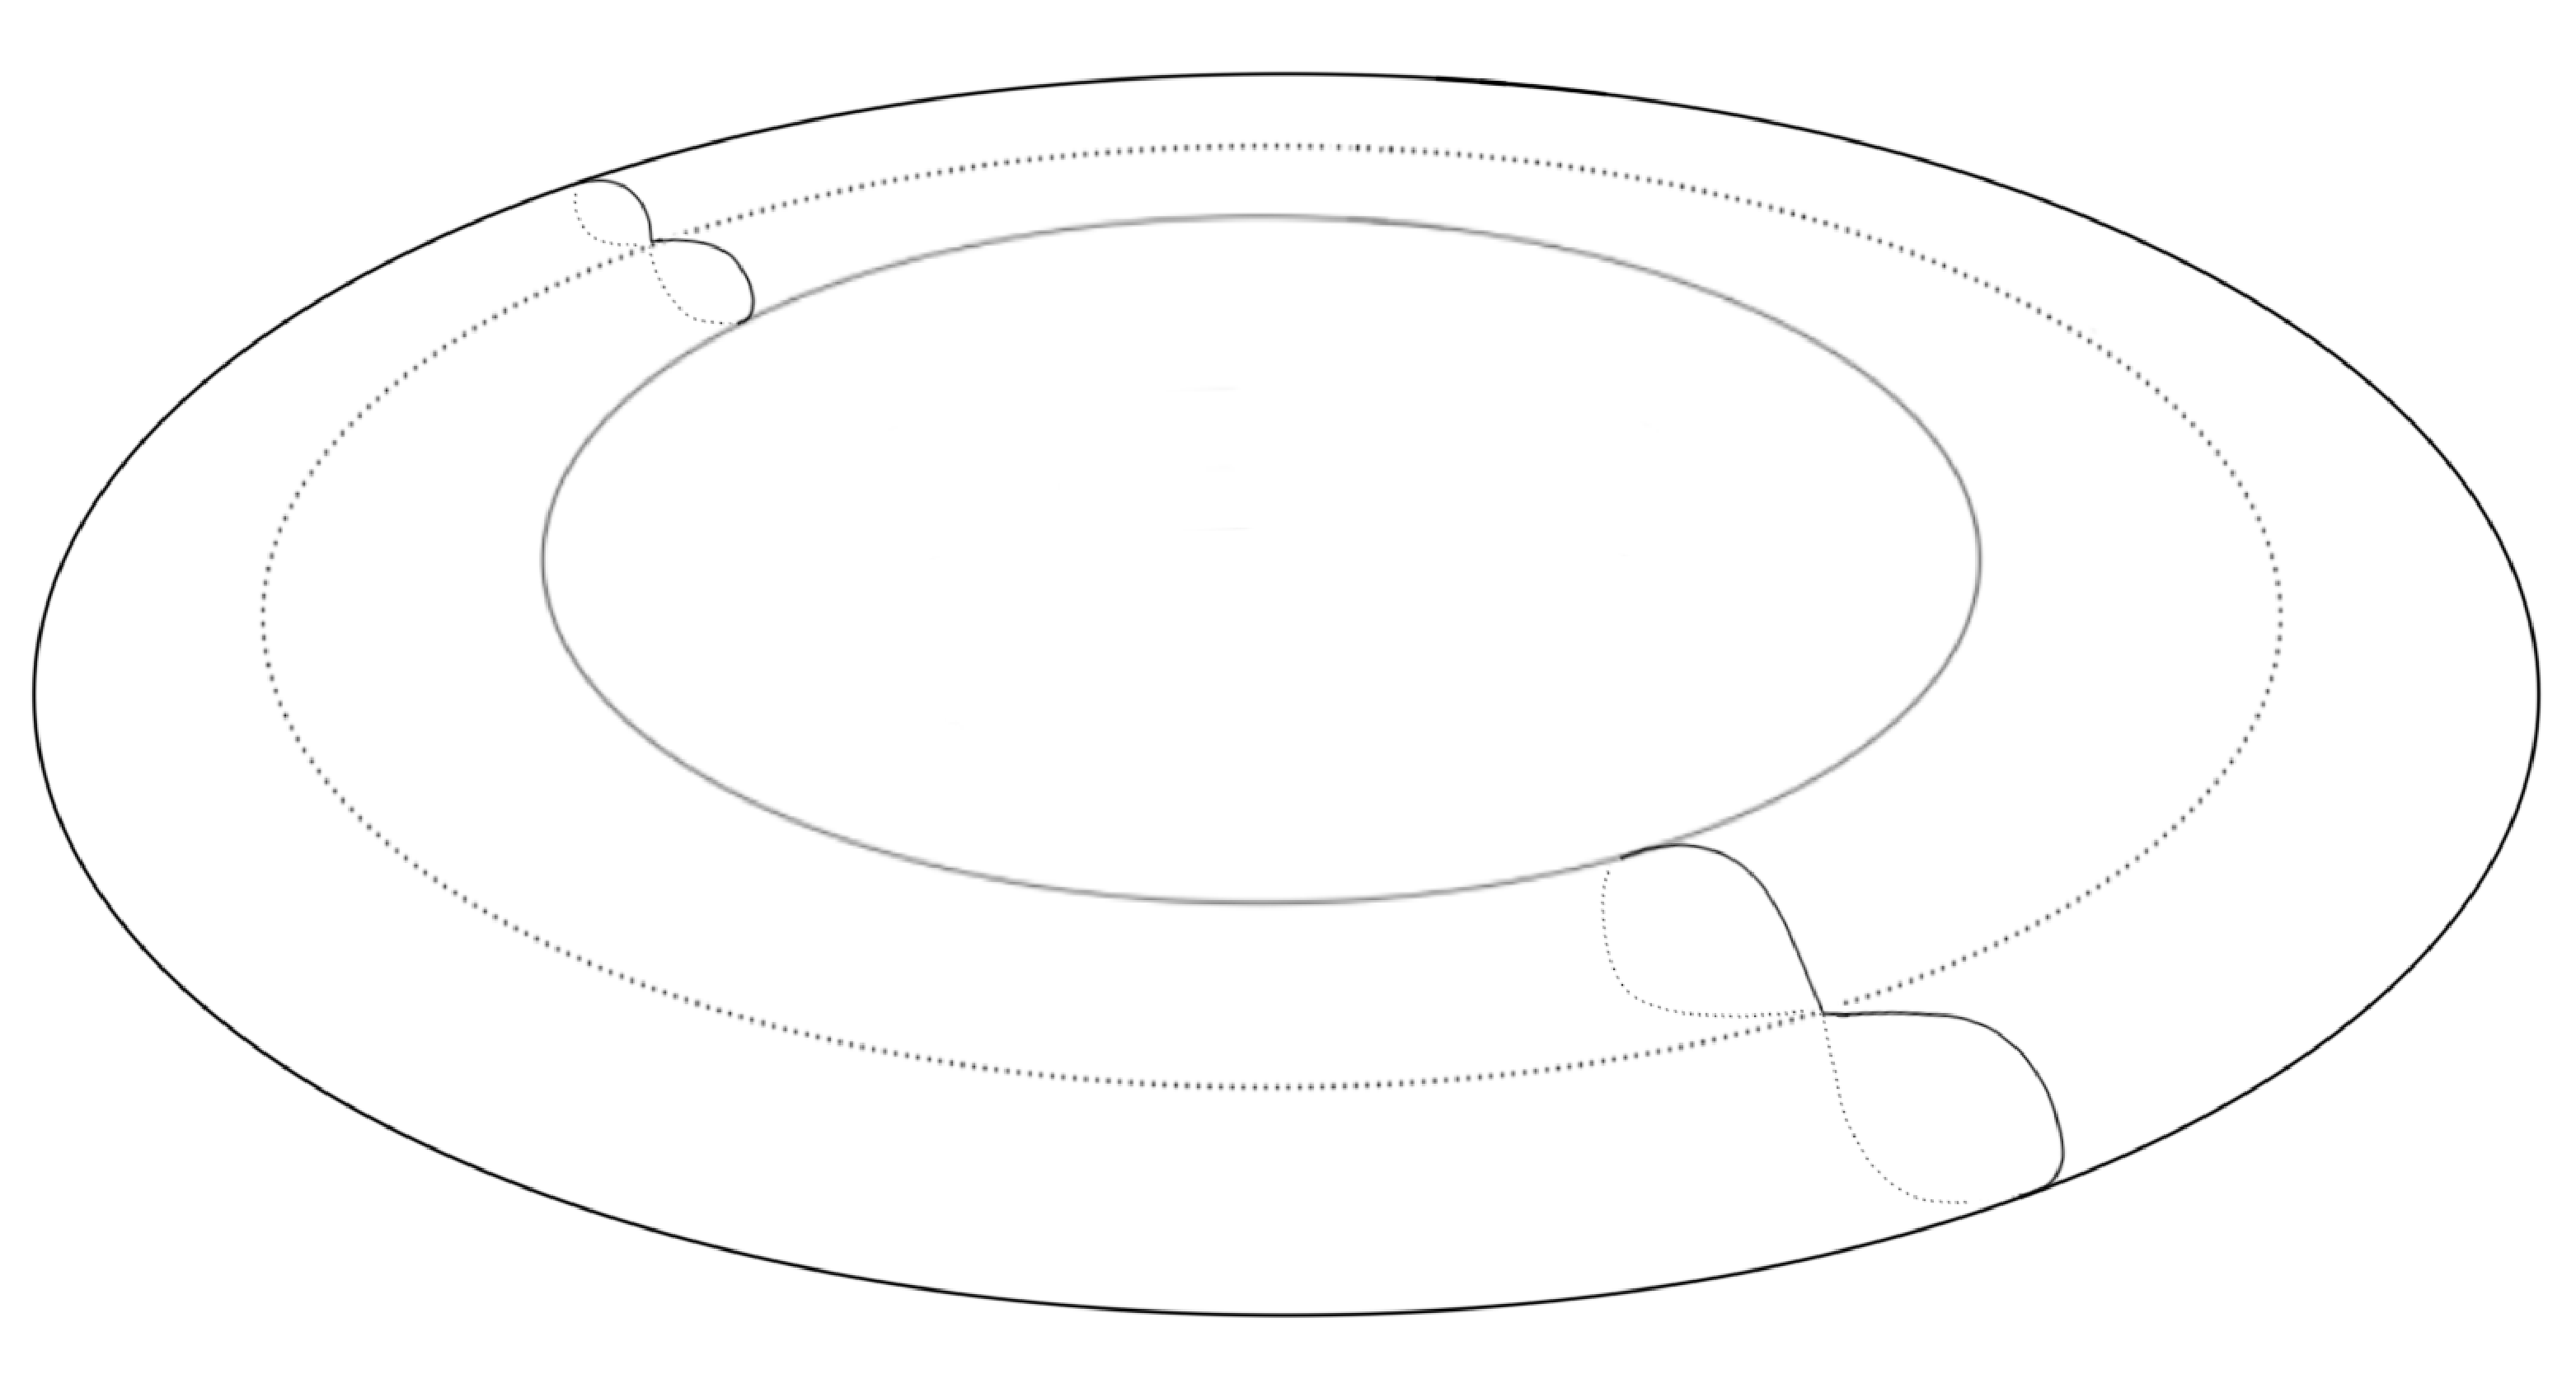
\includegraphics[scale=0.125]{images/section2/atoms/foc_ell_atom.pdf}
\caption{Поверхность уровня $\Xi = \const$ для перестройки 2.}
\label{fig:pt9:_foc_ell_atom}
\end{figure}

% \textcolor{red}{векторы в нижнем внутреннем эллипссе в \ref{fig:pt9:_domain_atom_foc_ell} определены неправильно. ВСЕ ПЕРЕДЕЛАТЬ}
 
%Соответствует случаю $\alpha_{in} = b^2, \ \alpha_{out} \in (\lambda_1, b^2)$.
%В этом случае каустика траектории во внешнем кольце $\Omega_{out}$ является эллипсом, а во внутренней области $\Omega_{in}$ интегральные траектории проходят вдоль прямых, которые содержат один из фокусов. 
%Векторы скоростей в области $\Omega_{in}$ и  $\Omega_{out}$ определим так же ранее (см. Рис. \ref{fig:pt9:_domain_atom_foc_ell}). 
%
%%При этом часть соединяющей фокусы прямой, которая попала в область $\Omega_{in}$, также рассмотрим как предельный случай софокусной гиперболы с устремленным к $b^2$ сверху параметром (см. Рис. \ref{fig:pt9:_atom1_result}). 
%Разрежем каждый лист $(\Omega, v_i), i=1,\ldots, 4$ вдоль горизонтальных пунктирных линий, соответствующих вырожденным гиперболам. 
%При этом разрез проходит в том числе через $\Omega_{out}$. 
%Пример листа склейки изображен на Рис. \ref{fig:pt9:_atom_foc_ell_leaf}.
%На Рис. \ref{fig:pt9:_atom_foc_ell_iter1}  изображен результат склейки листов $(\Omega, v_1)$ (на заднем плане) и $(\Omega, v_4)$ (на переднем плане). 
%Завершающие граничные восьмерки дуги склеиваются попарно, верхняя с нижней, по склейкам $\alpha$ и $\beta$. 
%Склейка листов $(\Omega, v_2)$ и $(\Omega, v_3)$ выглядит эквивалентно с точностью до обозначения листов.
%С обоих концов фигуры по <<андреевским крестам>> подклеивается результат склейки листов $(\Omega, v_2)$ и $(\Omega, v_3)$.
%На Рис. \ref{fig:pt9:_foc_ell_atom} изображена поверхность для особого значения интеграла: она состоит из двух торов, склеенных нетривиальным образом.

%
%\begin{figure}[!htb]
%\minipage{0.42\textwidth}
%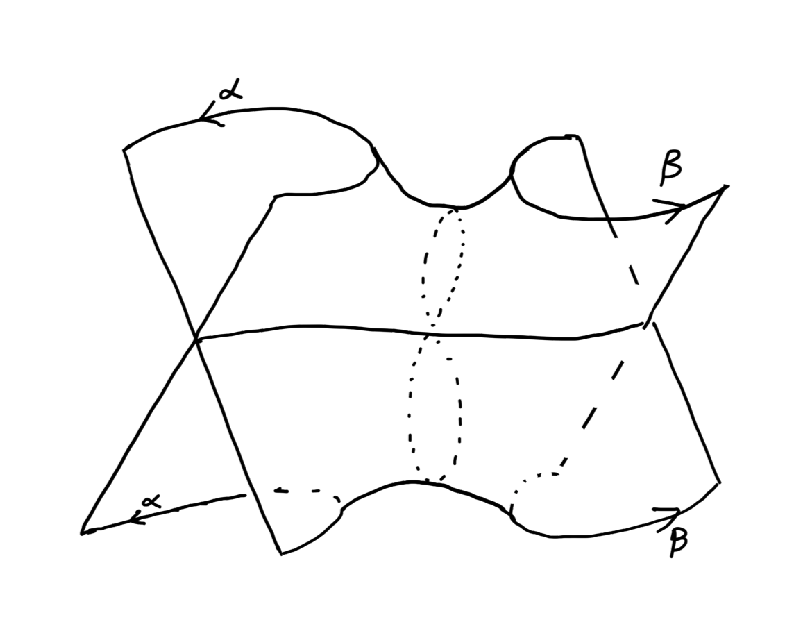
\includegraphics[scale=0.35]{images/section2/atoms/atom_foc_ell_iter1.pdf}
%\caption{Результат склейки $(\Omega, v_1)$ и $(\Omega, v_4)$.}
%\label{fig:pt9:_atom_foc_ell_iter1}
%\endminipage\hfill
%\minipage{0.43\textwidth}
%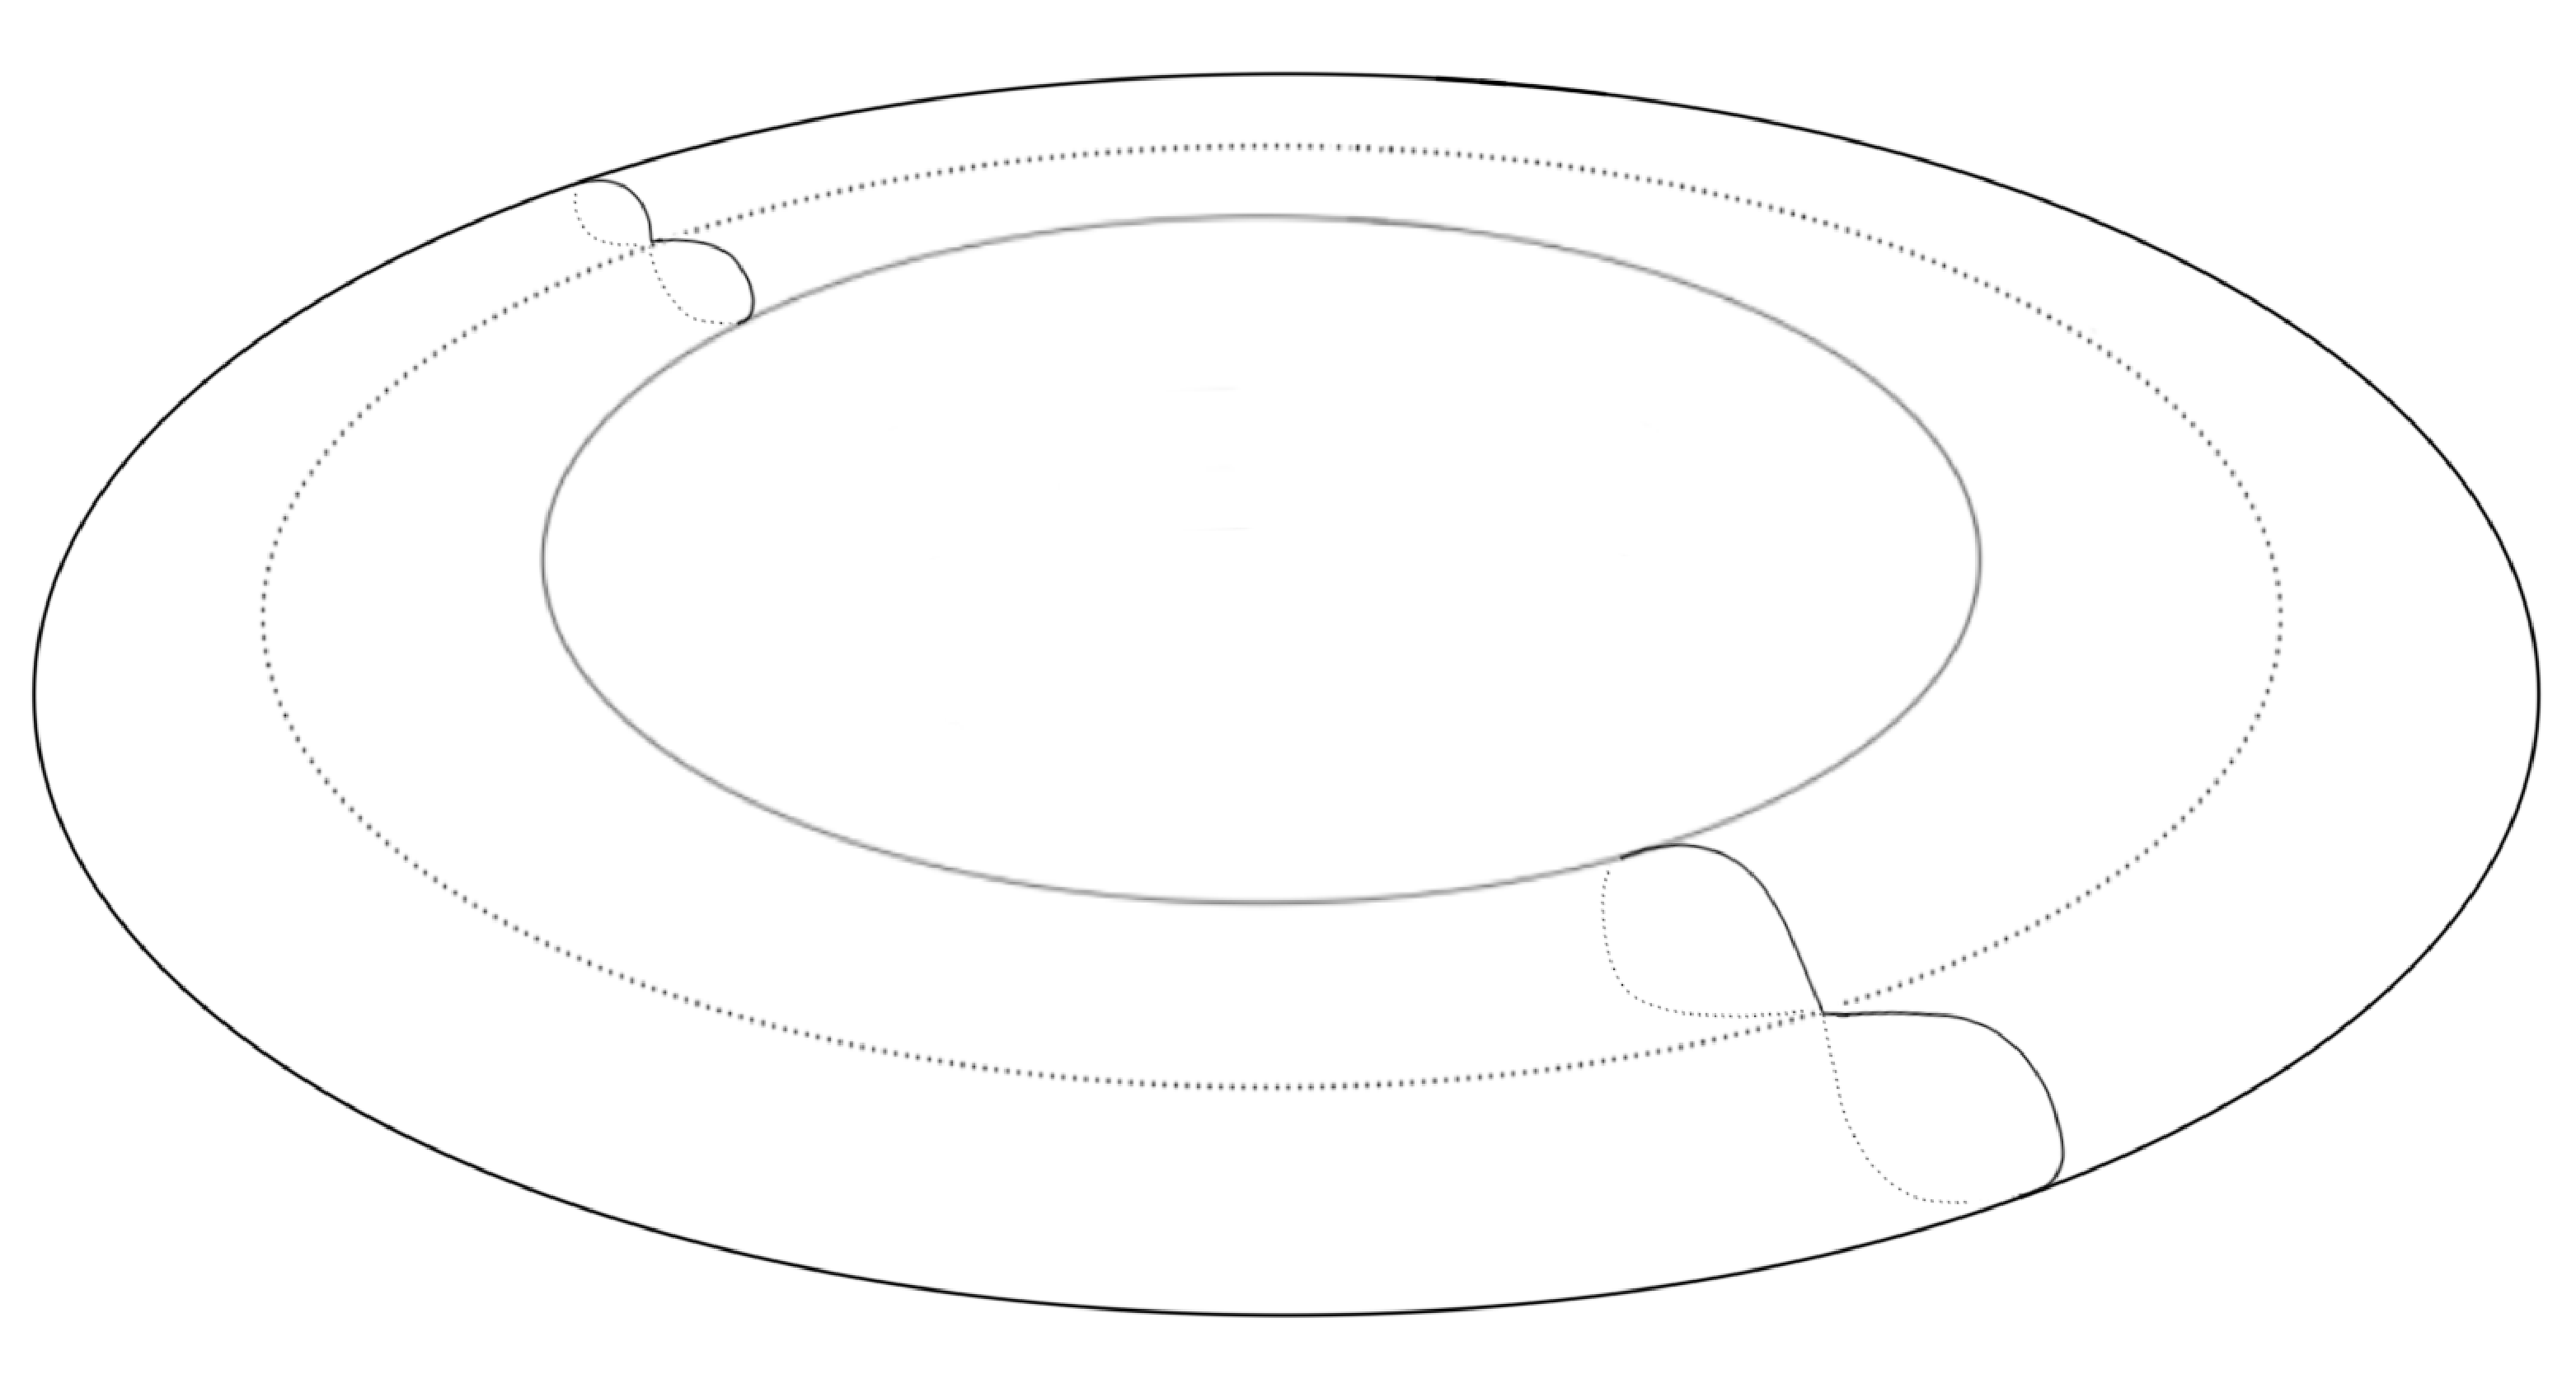
\includegraphics[scale=0.1]{images/section2/atoms/foc_ell_atom.pdf}
%\caption{Поверхность для особого значения $\Lambda=b^2 n_{in}^2$.}
%\label{fig:pt9:_foc_ell_atom}
%\endminipage\hfill
%\end{figure}

\textbf{Перестройка 3.}
Траектории бильярда в области $\Omega_{in}$ касаются эллипса с параметром $\alpha_{in}$, а в области $\Omega_{out}$ совпадают с вертикальной полуосью эллипса.

Поверхность $\Xi = \const$  можно представлять себе как предельный случай неособой поверхности $D_1^1$ (см. рис. \ref{fig:pt9:_diagramPlusIrregular}), когда две ручки <<схлопываются>> в окружности.

Более подробно, склеим листы $\widetilde{\Omega}_1$ и $\widetilde{\Omega}_4$ по общим границам, которые проецируются в эллиптические граничные дуги $\widetilde{\Omega}$ (пример области $\widetilde{\Omega}_1$ изображен на рис. \ref{fig:pt9:_hyp_page}). Аналогично для 
$\widetilde{\Omega}_2$ и $\widetilde{\Omega}_3$. Результатом склейки являются два тора с четыремя дырками каждый. При этом каждая дырка ограничена двумя дугами, которые проецируются в гиперболические граничные дуги области $\widetilde{\Omega}$. 

Области $\widetilde{\Omega}_1$ и $\widetilde{\Omega}_2$ отождествляются по дугам общей границы, которые проектируются в гиперболические граничные дуги области $\widetilde{\Omega}$, аналогично для областей $\widetilde{\Omega}_3$ и $\widetilde{\Omega}_4$. 
%В целях наглядности проденем граничные окружности друг через друга в компонентах, которые проекция $\pi$ отображает  в область $\widetilde{\Omega}_{out}$ (см. рис. \ref{fig:pt9:_atom_3_step}). Аналогично поступим с областями $\widetilde{\Omega}_2$ и $\widetilde{\Omega}_3$. 
\begin{figure}[!htb]
\minipage{0.48\textwidth}
\centering
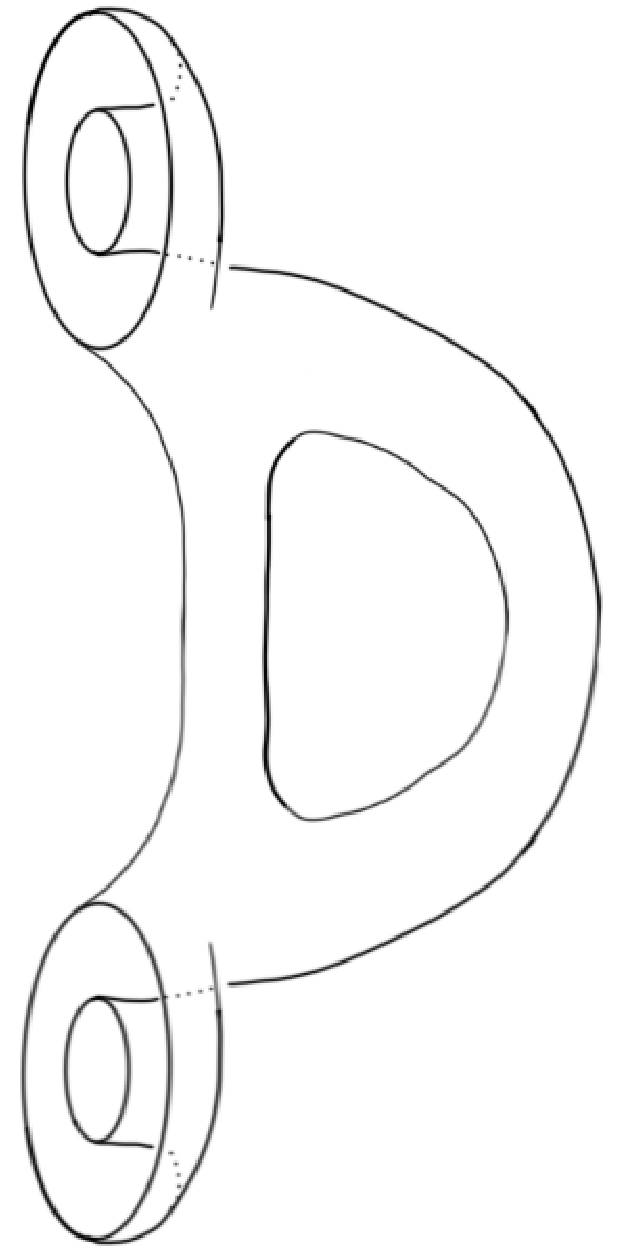
\includegraphics[scale=0.2]{images/section2/atoms/atom_3_step.pdf}
    \caption{Склейка $\widetilde{\Omega}_1 \cup \widetilde{\Omega}_4$ (перестройка 3).}
    \label{fig:pt9:_atom_3_step}
\endminipage\hfill
\minipage{0.52\textwidth}
\centering
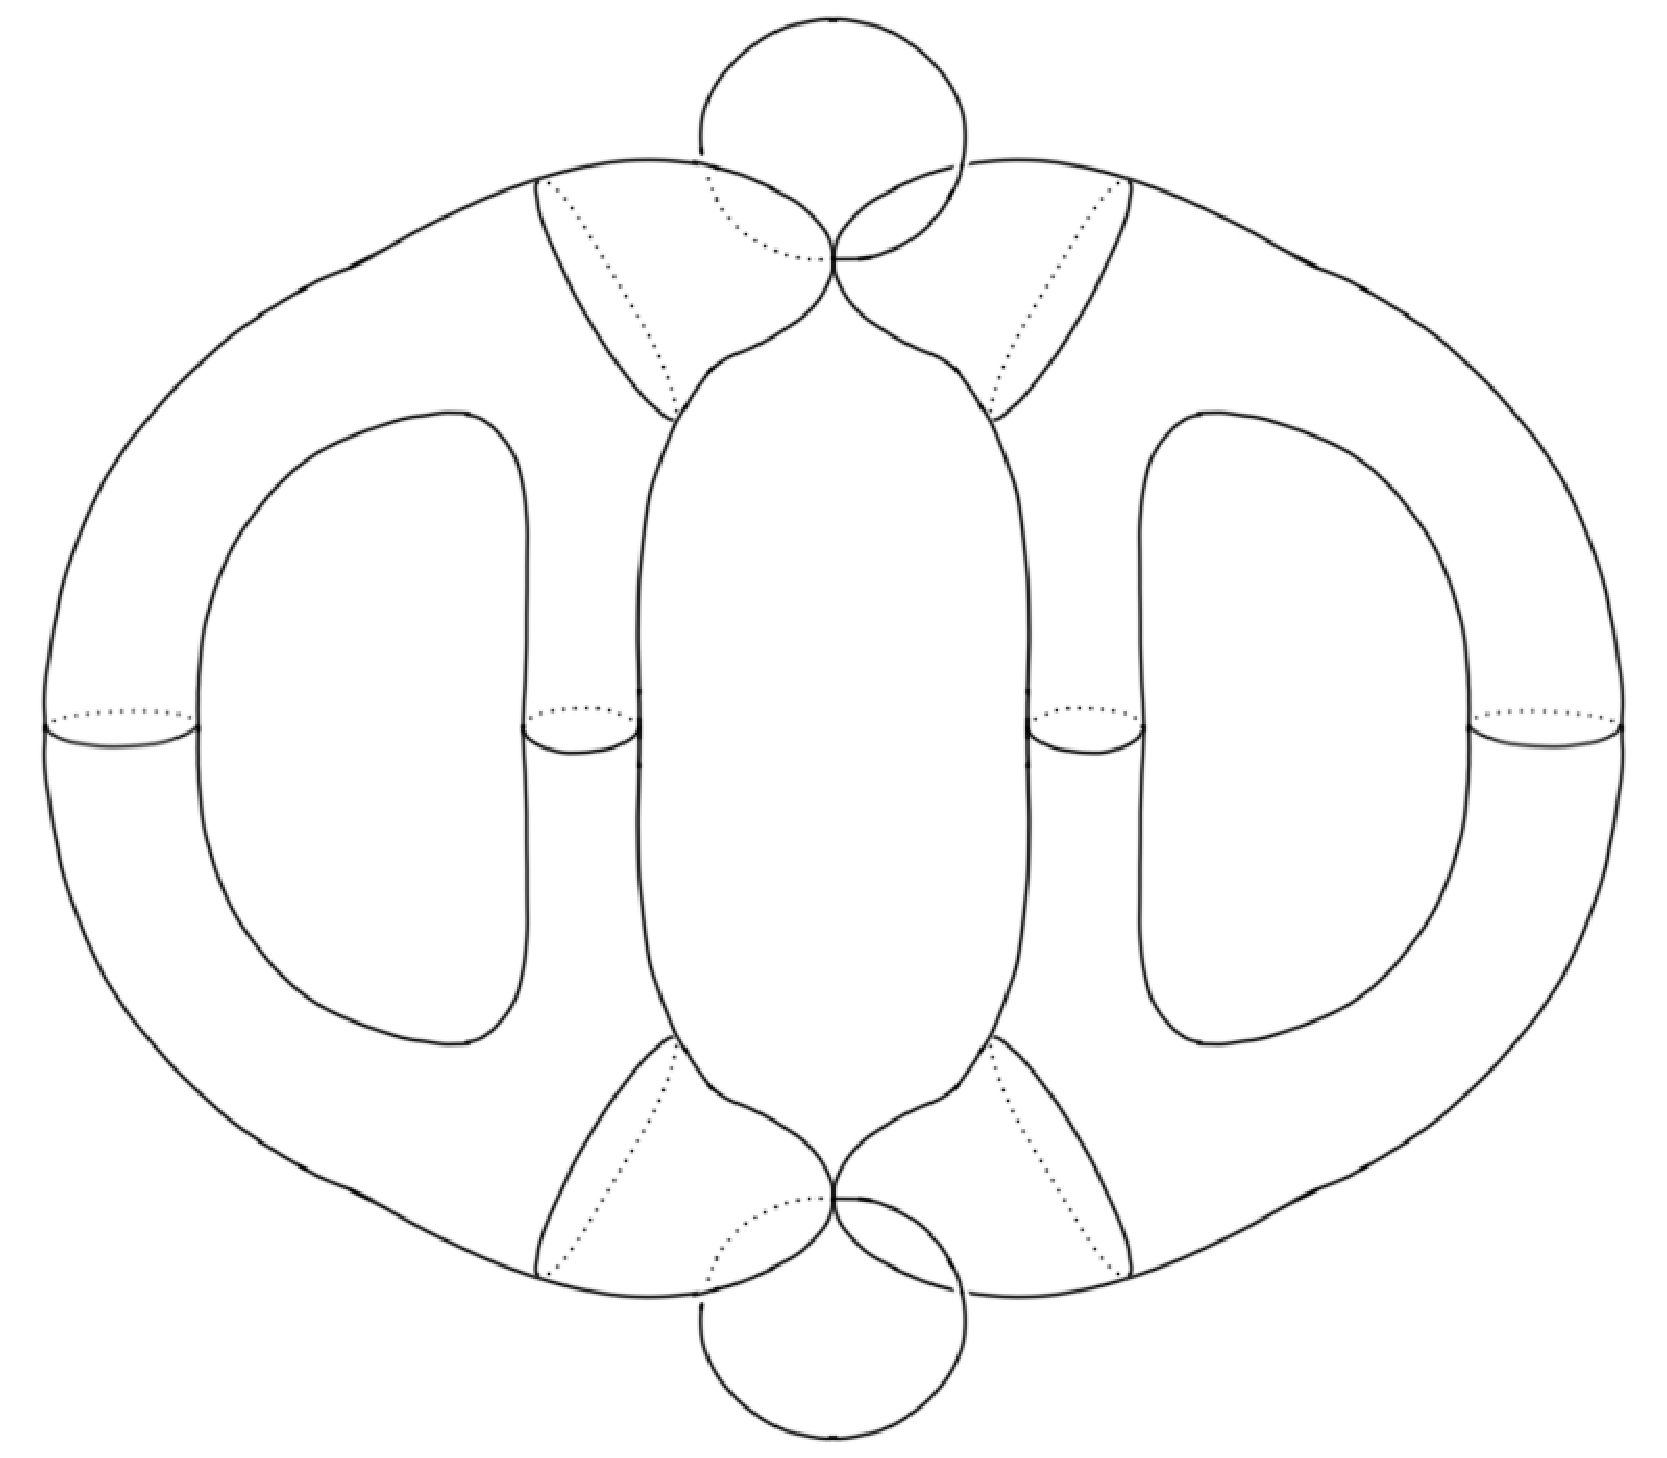
\includegraphics[scale=0.2]{images/section2/atoms/atom_3.pdf}
    \caption{Поверхность уровня $\Xi = \const$ для перестройки 3.}
    \label{fig:pt9:_atom_3}
\endminipage\hfill
\end{figure}

На рис. \ref{fig:pt9:_atom_3_step} изобразим результат склейки $\widetilde{\Omega}_1 \cup \widetilde{\Omega}_4$. Его границей являются две пары окружностей, по которым приклеивается  аналогичный результат склейки $\widetilde{\Omega}_2 \cup \widetilde{\Omega}_3$.
%К левым (внешним) окружностям $\widetilde{\Omega}_1 \cup \widetilde{\Omega}_4$ подклеим соответствующие на $\widetilde{\Omega}_2 \cup \widetilde{\Omega}_3$, а также склеим полученные поверхности по правым (внутренним). 
В момент перестройки две верхние (соответственно, две нижние) граничные окружности  $\widetilde{\Omega}_1 \cup \widetilde{\Omega}_4$ стягиваются в одну окружность. То есть поверхность $\Xi = \const$ представляет собой два касающихся в двух точках тора, при этом в каждой общей точке этих двух торов <<растет>> по одной окружности, см.  рис. \ref{fig:pt9:_atom_3}. 

\textbf{Перестройка 4.} 
Траектории бильярда в области $\Omega_{in}$ лежат на проходящих через фокусы прямых, а продолжения звеньев в области $\Omega_{out}$ касаются гиперболы с параметром $\alpha_{out}$. 

Определим область $\widetilde{\Omega}$  как объединение $\Omega_{in}$ и $\widetilde{\Omega}_{out}$, где область $\widetilde{\Omega}_{out}$ определена как пересечение $\Omega_{out}$ с областью, лежащей  между ветвями гиперболы с параметром $\alpha_{out}$. 

Горизонтальная ось пересекает область $\Omega_{in}$ по трем отрезкам, один из которых соединяет фокусы. Разрежем область $\widetilde{\Omega}$ горизонтальной осью. 
Тогда можем определить разбиение области $\widetilde{\Omega}$ на четыре области 
$\widetilde{\Omega}_{out}^u, \Omega_{in}^u, \Omega_{in}^d, \widetilde{\Omega}_{out}^d$. 
Проекция $\pi$ четырехлистна в каждой  внутренней точке любой из этих областей. Обозначим прообразы этих областей на поверхности $\Xi = \const$ как 
$\widetilde{\Omega}_{out,j}^u, \Omega_{in, j}^u, \Omega_{in, j}^d, \widetilde{\Omega}_{out, j}^d, j=1, \ldots, 4$.
Области $\Omega_{in, j}^u, \Omega_{in, j}^d, j=1,\ldots,4$ занумерованы в соответствии с правилом \eqref{eq:foc_numeration}, а области $\widetilde{\Omega}_{out,j}^u, \widetilde{\Omega}_{out, j}^d, 1, \ldots, 4$ --- как на рис. \ref{fig:pt9:_hyp_vectors_numbering}.

Области $\widetilde{\Omega}_{out,j}^u$ и $\Omega_{in, j}^u$ на поверхности $\Xi = \const$ для каждого $j=1, \ldots, 4$ отождествляются по общей границе, которая на $\widetilde{\Omega}$ проектируется в часть дуги эллипса $Q_{\lambda_1}$, заключенная между ветвями гиперболы $Q_{\alpha_{out}}$ в верхней полуплоскости. В симметричную ей дугу в нижней полуплоскости проектируется общая граница для областей $\widetilde{\Omega}_{out,1}^d$ и $\Omega_{in, 4}^d$. Аналогичным образом отождествляются дуги на границах областей $\widetilde{\Omega}_{out,2}^d$ и $\Omega_{in, 3}^d$, $\widetilde{\Omega}_{out,3}^d$ и $\Omega_{in, 2}^d$, а также $\widetilde{\Omega}_{out,4}^d$ и $\Omega_{in, 1}^d$.

В соединяющий фокусы отрезок проектируется общая граница для областей $\Omega_{in, 1}^u, \Omega_{in, 1}^d, \Omega_{in, 4}^u, \Omega_{in, 4}^d$, аналогично для областей $\Omega_{in, 2}^u, \Omega_{in, 2}^d, \Omega_{in, 3}^u, \Omega_{in, 3}^d$.
На той же прямой можно выделить отрезки, которые соединяют правый фокус с правой вершиной эллипса $Q_{\lambda_1}$. На каждый из этих отрезков проектируются границы областей $\Omega_{in, 1}^u, \Omega_{in, 2}^d, \Omega_{in, 1}^d, \Omega_{in, 2}^u$, аналогично для областей $\Omega_{in, 3}^u, \Omega_{in, 4}^d, \Omega_{in, 3}^d, \Omega_{in, 4}^u$.

Определим листы склейки $\widetilde{\Omega}_1, \ldots, \widetilde{\Omega}_4$ следующим образом (пример области $\widetilde{\Omega}_1$ см. рис. \ref{fig:pt9:_atom_4_domain}):
\begin{equation}
\begin{array}{cc}
\widetilde{\Omega}_1 = \widetilde{\Omega}_{out, 1}^u \cup \Omega_{in, 1}^u \cup \Omega_{in, 4}^d \cup \widetilde{\Omega}_{out, 1}^d, &
\widetilde{\Omega}_2 = \widetilde{\Omega}_{out, 2}^u \cup \Omega_{in, 2}^u \cup \Omega_{in, 3}^d \cup \widetilde{\Omega}_{out, 2}^d, \\
\widetilde{\Omega}_3 = \widetilde{\Omega}_{out, 3}^u \cup \Omega_{in, 3}^u \cup \Omega_{in, 2}^d \cup \widetilde{\Omega}_{out, 3}^d, &
\widetilde{\Omega}_4 = \widetilde{\Omega}_{out, 4}^u \cup \Omega_{in, 4}^u \cup \Omega_{in, 1}^d \cup \widetilde{\Omega}_{out, 4}^d.
\end{array}
\label{eq:case4Omegas}
\end{equation}
\begin{figure}[!htb]
\centering
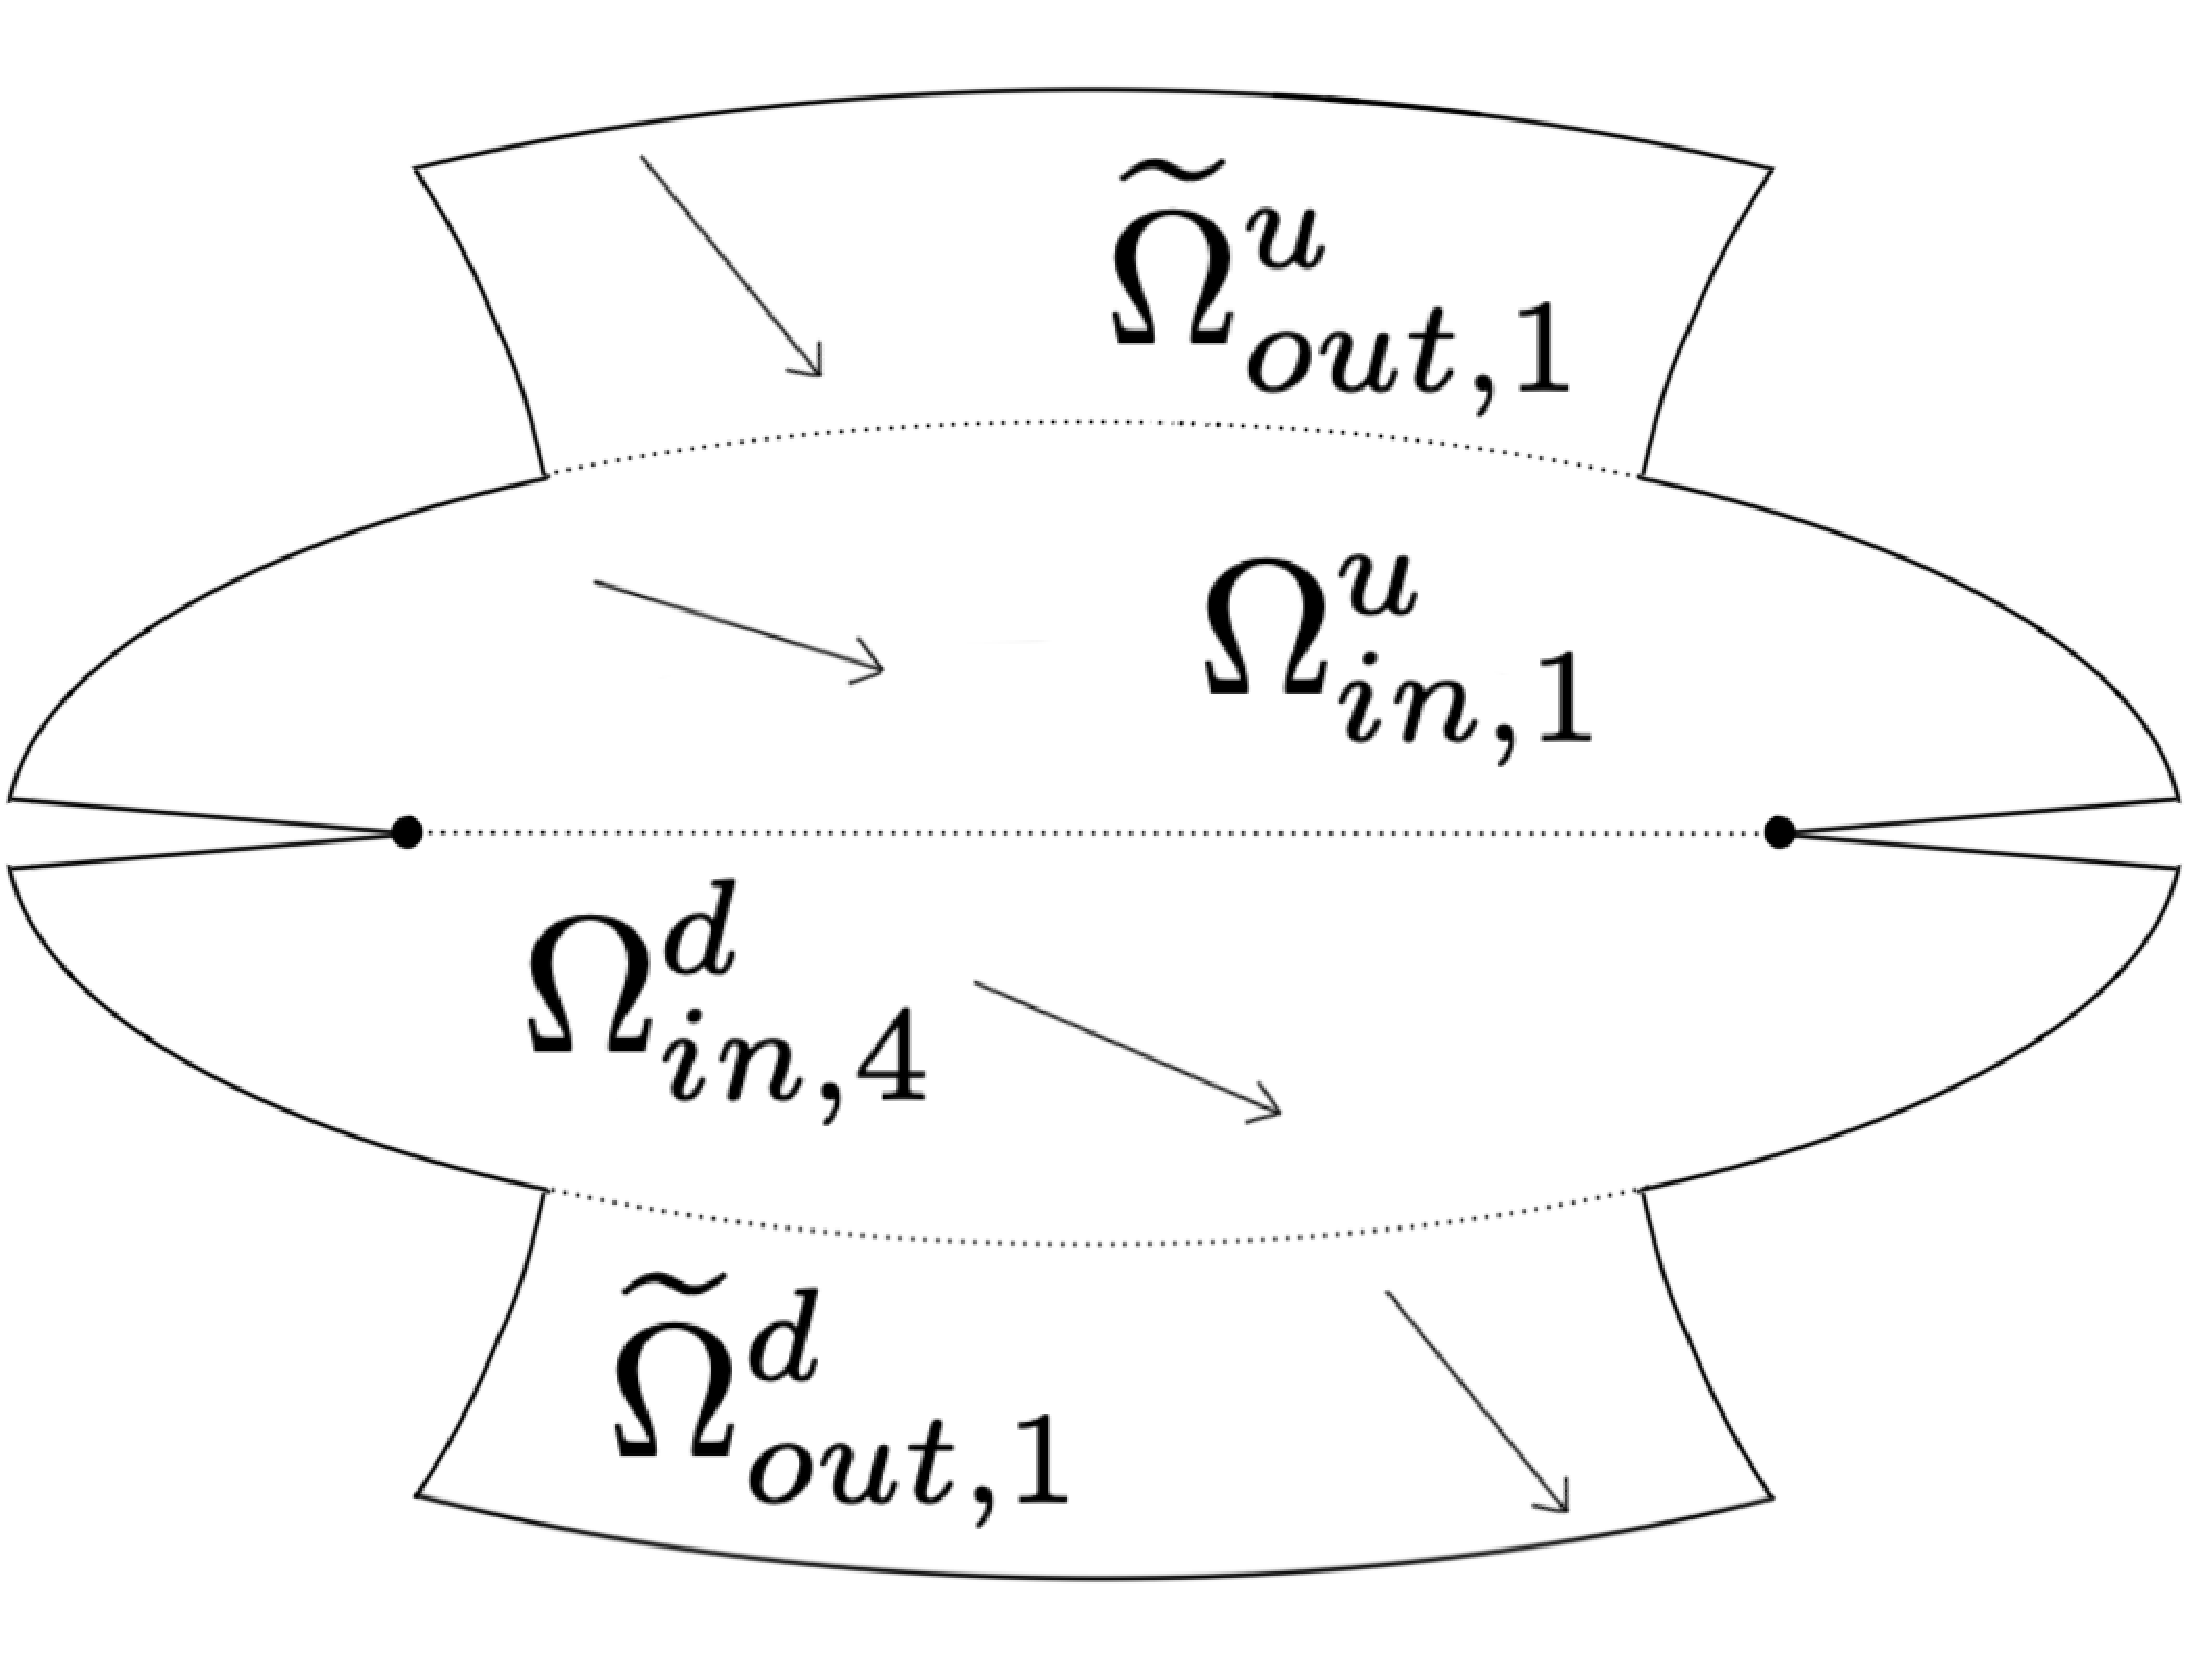
\includegraphics[width=5cm]{images/section2/atoms/atom_4_domain.pdf}
    \caption{Пример области $\widetilde{\Omega}_1$ для перестройки 4.}
    \label{fig:pt9:_atom_4_domain}
\end{figure}


Склеим листы $\widetilde{\Omega}_1$ и  $\widetilde{\Omega}_4$ по общим граничным дугам на поверхности $\Xi = \const$, которые проецируются на эллиптические граничные дуги области $\widetilde{\Omega}$, а также на  
%проецирующимся в эллиптические . Точнее, по двум дугам, проектирующимся на граничный эллипс между ветвей гиперболы $Q_{\alpha_{out}}$, а также по дугам, проектирующимися на  эллипс $Q_{\lambda_1}$ вне указанных ветвей. 
%Листы $\widetilde{\Omega}_1$ и  $\widetilde{\Omega}_4$ также склеим по граничной дуге на поверхности, которая проектируется на 
соединяющий фокусы отрезок. Аналогичные склейки повторим для листов $\widetilde{\Omega}_2$ и  $\widetilde{\Omega}_3$. Результатом склеек являются две фигуры, каждая из которых является склейкой цилиндров с двумя дырками вдоль общей горизонтальной направляющей (см. рис. \ref{fig:pt9:_atom_foc_hyp_iter1}).


Ветви гиперболы с параметром $\alpha_{out}$ пересекаются с областью $\widetilde{\Omega}_{out}$ по четырем дугам, в каждую из которых проектируются по две дуги на $\Xi = \const$, ограничивающие одну из дырок на склейке $\widetilde{\Omega}_1 \cup \widetilde{\Omega}_4$. Аналогично для склейки $\widetilde{\Omega}_2 \cup \widetilde{\Omega}_3$. При этом на дуги в верхней полуплоскости проектируются общие границы для $\widetilde{\Omega}_{out, 1}^u$ и $\widetilde{\Omega}_{out, 4}^u$, а также $\widetilde{\Omega}_{out, 2}^u$ и $\widetilde{\Omega}_{out, 3}^u$. Аналогичные склейки для $\widetilde{\Omega}_{out, 1}^d$ и $\widetilde{\Omega}_{out, 4}^d$, а также $\widetilde{\Omega}_{out, 2}^d$ и $\widetilde{\Omega}_{out, 3}^d$ возникают на прообразе дуг в нижней полуплоскости.

Граничные окружности цилиндров проецируются на отрезки $\{y=0\} \cap \Omega_{in}$ вне фокусов. Точнее, в правый такой отрезок проектируются пары дуг $\Omega_{in, 1}^u \cap \Omega_{in, 4}^u$, $\Omega_{in, 1}^d \cap \Omega_{in, 4}^d$, которые ограничивают верхнюю и нижнюю граничные окружности, соответственно. Аналогично для пар дуг $\Omega_{in, 2}^u \cap \Omega_{in, 3}^u$, $\Omega_{in, 2}^d \cap \Omega_{in, 3}^d$. 
По этим граничным окружностям склеим также возникают склейки $\widetilde{\Omega}_1 \cup \widetilde{\Omega}_4$ и $\widetilde{\Omega}_2 \cup \widetilde{\Omega}_3$. 
Торцевые окружности при этом в правой части подклеиваются с <<перекруткой>>: \textit{нижняя} граничная окружность $\widetilde{\Omega}_1 \cup \widetilde{\Omega}_4$ отождествляется с \textit{верхней} окружностью на $\widetilde{\Omega}_2 \cup \widetilde{\Omega}_3$, аналогично \textit{верхняя} на $\widetilde{\Omega}_1 \cup \widetilde{\Omega}_4$ --- с \textit{нижней} на $\widetilde{\Omega}_2 \cup \widetilde{\Omega}_3$.
Аналогичные соображения для тех же листов справедливы в симметричном отрезке в левой полуплоскости.

Остается склеить отождествить $\widetilde{\Omega}_1 \cup \widetilde{\Omega}_4$ и $\widetilde{\Omega}_2 \cup \widetilde{\Omega}_3$ по указанным дугам (см. рис. \ref{fig:pt9:_atom_foc_hyp_iter1}).
%
%
%Соответствует случаю $\alpha_{in} = b^2, \ \alpha_{out} \in (b^2, a^2)$. 
%Область приведена на Рис. \ref{fig:pt9:_atom_4_domain}. В области $\Omega_{out}$ траектории касаются гиперболы, а во внутренней области $\Omega_{in}$ --- направлены к одному из фокусов. 
%Повторяя изложенные выше соображения, разрежем ту часть области $\Omega$, в которой траектории направлены к одному из фокусов, по отрезкам от фокуса до внешней эллиптической границы. 
%При этом на соединяющем фокусы отрезке появится склейка первого и четвертого листов. Результат после этой склейки изображен на Рис. \ref{fig:pt9:_atom_foc_hyp_iter1}
Результирующая поверхность $\Xi = \const$ изображена на рис. \ref{fig:pt9:_atom_4}.

\begin{figure}[!htb]
\minipage{0.5\textwidth}
\centering
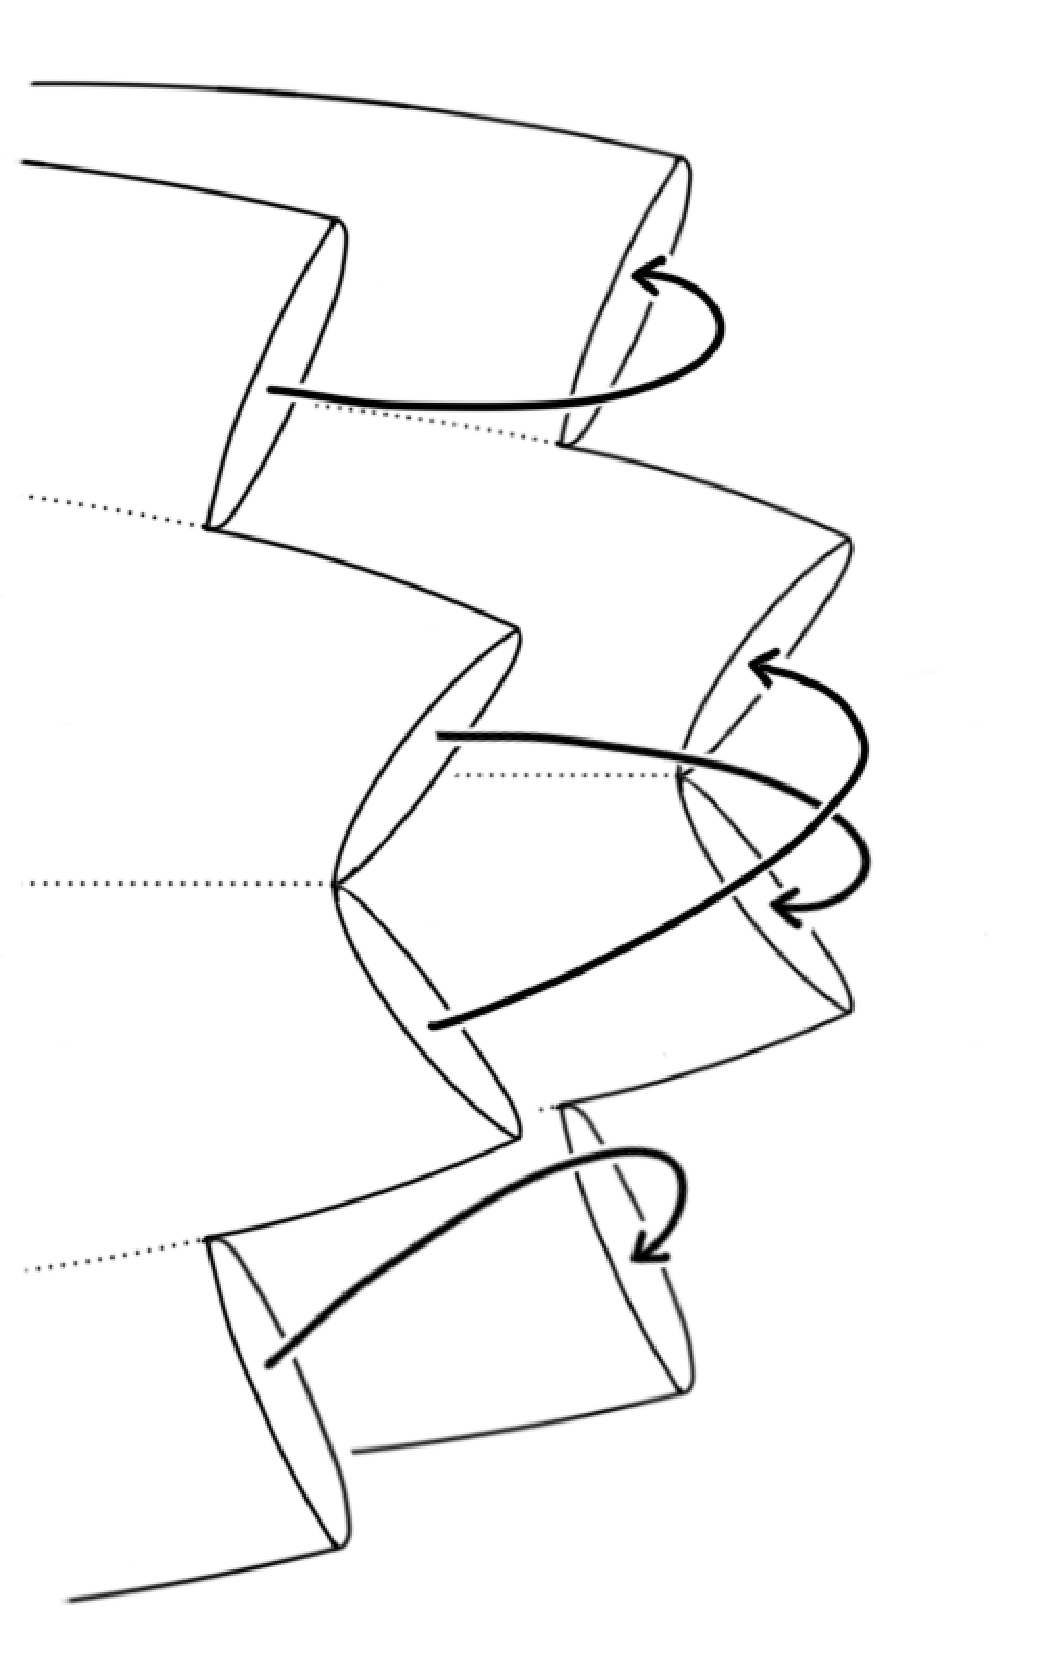
\includegraphics[width=3cm]{images/section2/atoms/atom_foc_hyp_iter1.pdf}
    \caption{Схема склейки $\widetilde{\Omega}_1 \cup \widetilde{\Omega}_4$ (на переднем плане) и $\widetilde{\Omega}_2 \cup \widetilde{\Omega}_3$ (на заднем плане).}
    \label{fig:pt9:_atom_foc_hyp_iter1}
    \endminipage\hfill
\minipage{0.5\textwidth}
    \centering
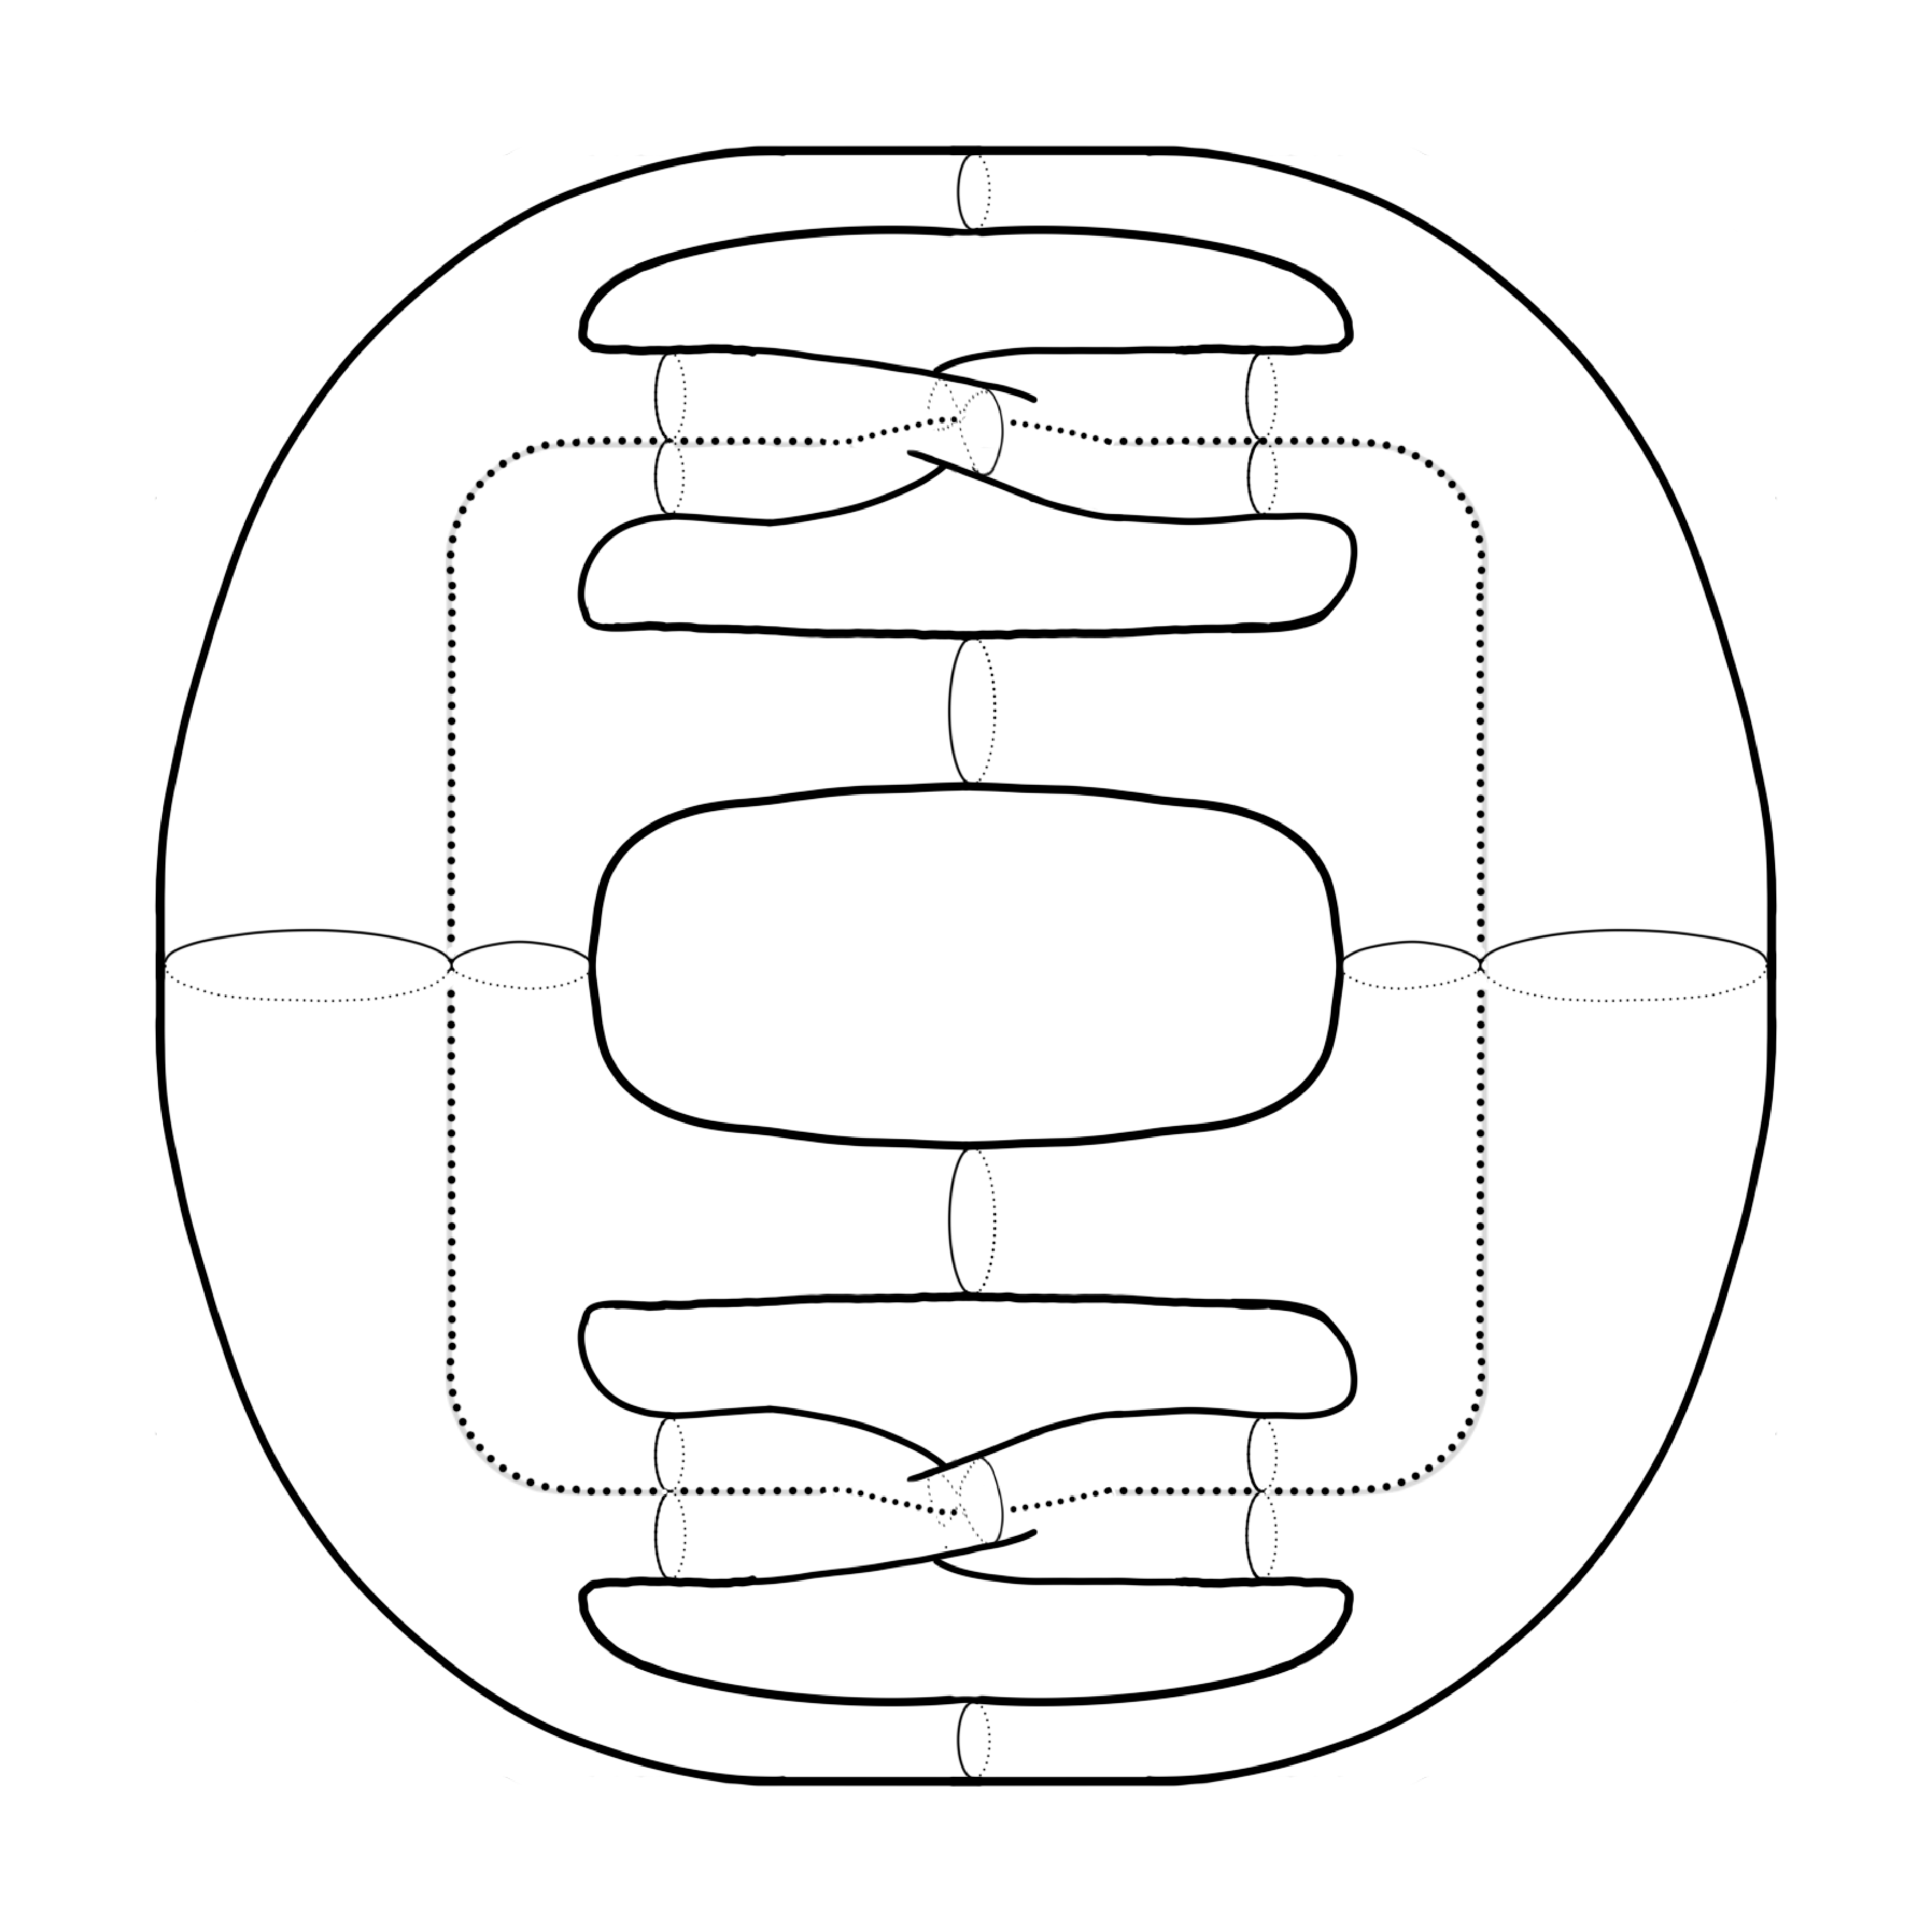
\includegraphics[width=5cm]{images/section2/atoms/atom_4.pdf}
    \caption{Поверхность уровня $\Xi = \const$ для перестройки 4.}
    \label{fig:pt9:_atom_4}
\endminipage\hfill
\end{figure}

\textbf{Перестройка 5.} 
Звенья траектории в области $\Omega_{in}$ касаются гиперболы с параметром $\alpha_{in}$, а в области $\Omega_{out}$ лежат на проходящих через фокусы прямых.

Определим область $\widetilde{\Omega}_{in}$ как часть эллипса $\Omega_{in}$ между ветвей гиперболы с параметром $\alpha_{in}$. 
Область $\widetilde{\Omega}$ определим как объединение $\widetilde{\Omega}_{in} \cup \Omega_{out}$.

Проекция поверхности $\Xi = \const$ на область $\widetilde{\Omega}$ четырехлистна в каждой внутренней точке $\widetilde{\Omega}$ кроме отрезков $\Omega_{out} \cap \{y=0\}$.
Разрежем $\Omega_{out}$ вдоль этих горизонтальных отрезков и получим области $\Omega_{out}^u,  \Omega_{out}^d$. 
Тогда проекция четырехлистна в каждой области $\widetilde{\Omega}_{in}, \Omega_{out}^u,  \Omega_{out}^d$. Прообразы этих областей на поверхности $\Xi = \const$  обозначим как $\widetilde{\Omega}_{in, j}, \Omega_{out, j}^u,  \Omega_{out, j}^d, j=1,\ldots, 4$. 
При этом области $\Omega_{out, j}^u,  \Omega_{out, j}^d$ занумерованы  в соответствии с правилом \eqref{eq:foc_numeration}, а области $\widetilde{\Omega}_{in, j}$ --- как на рис. \ref{fig:pt9:_hyp_vectors_numbering}.

На поверхности $\Xi = \const$ области $\widetilde{\Omega}_{in, j}$ и $\Omega_{out, j}^u$ для каждого $j=1, \ldots,4$  отождествляются по дуге, которая проектируется в $\widetilde{\Omega}$ на дугу эллипса $Q_{\lambda_1}$, заключенную между ветвями гиперболы с параметром $\alpha_{in}$ в верхней полуплоскости. На симметричную дугу в нижней полуплоскости проектируются общие граничные дуги для областей $\widetilde{\Omega}_{in, 1}$ и $\Omega_{out, 4}^d$, аналогично для пары областей $\widetilde{\Omega}_{in, 2}$ и $\Omega_{out, 3}^d$, для пары $\widetilde{\Omega}_{in, 3}$ и $\Omega_{out, 2}^d$, а также для пары $\widetilde{\Omega}_{in, 4}$ и $\Omega_{out, 1}^d$. 

Определим листы $\widetilde{\Omega}_1, \ldots, \widetilde{\Omega}_4$. 
\begin{equation}
\begin{array}{cc}
\widetilde{\Omega}_1 = \Omega_{out, 1}^u \cup \widetilde{\Omega}_{in, 1} \cup \Omega_{out, 4}^d, &
\widetilde{\Omega}_2 = \Omega_{out, 2}^u \cup \widetilde{\Omega}_{in, 2} \cup \Omega_{out, 3}^d, \\
\widetilde{\Omega}_3 = \Omega_{out, 3}^u \cup \widetilde{\Omega}_{in, 3} \cup \Omega_{out, 2}^d, &
\widetilde{\Omega}_4 = \Omega_{out, 4}^u \cup \widetilde{\Omega}_{in, 4} \cup \Omega_{out, 1}^d.
\end{array}
\label{eq:case5Omegas}
\end{equation}
Пример области $\widetilde{\Omega}_1$ изображен на рис. \ref{fig:pt9:_domain_atom_hyp_foc}.

\begin{figure}[!htb]
\minipage{0.5\textwidth}
\centering
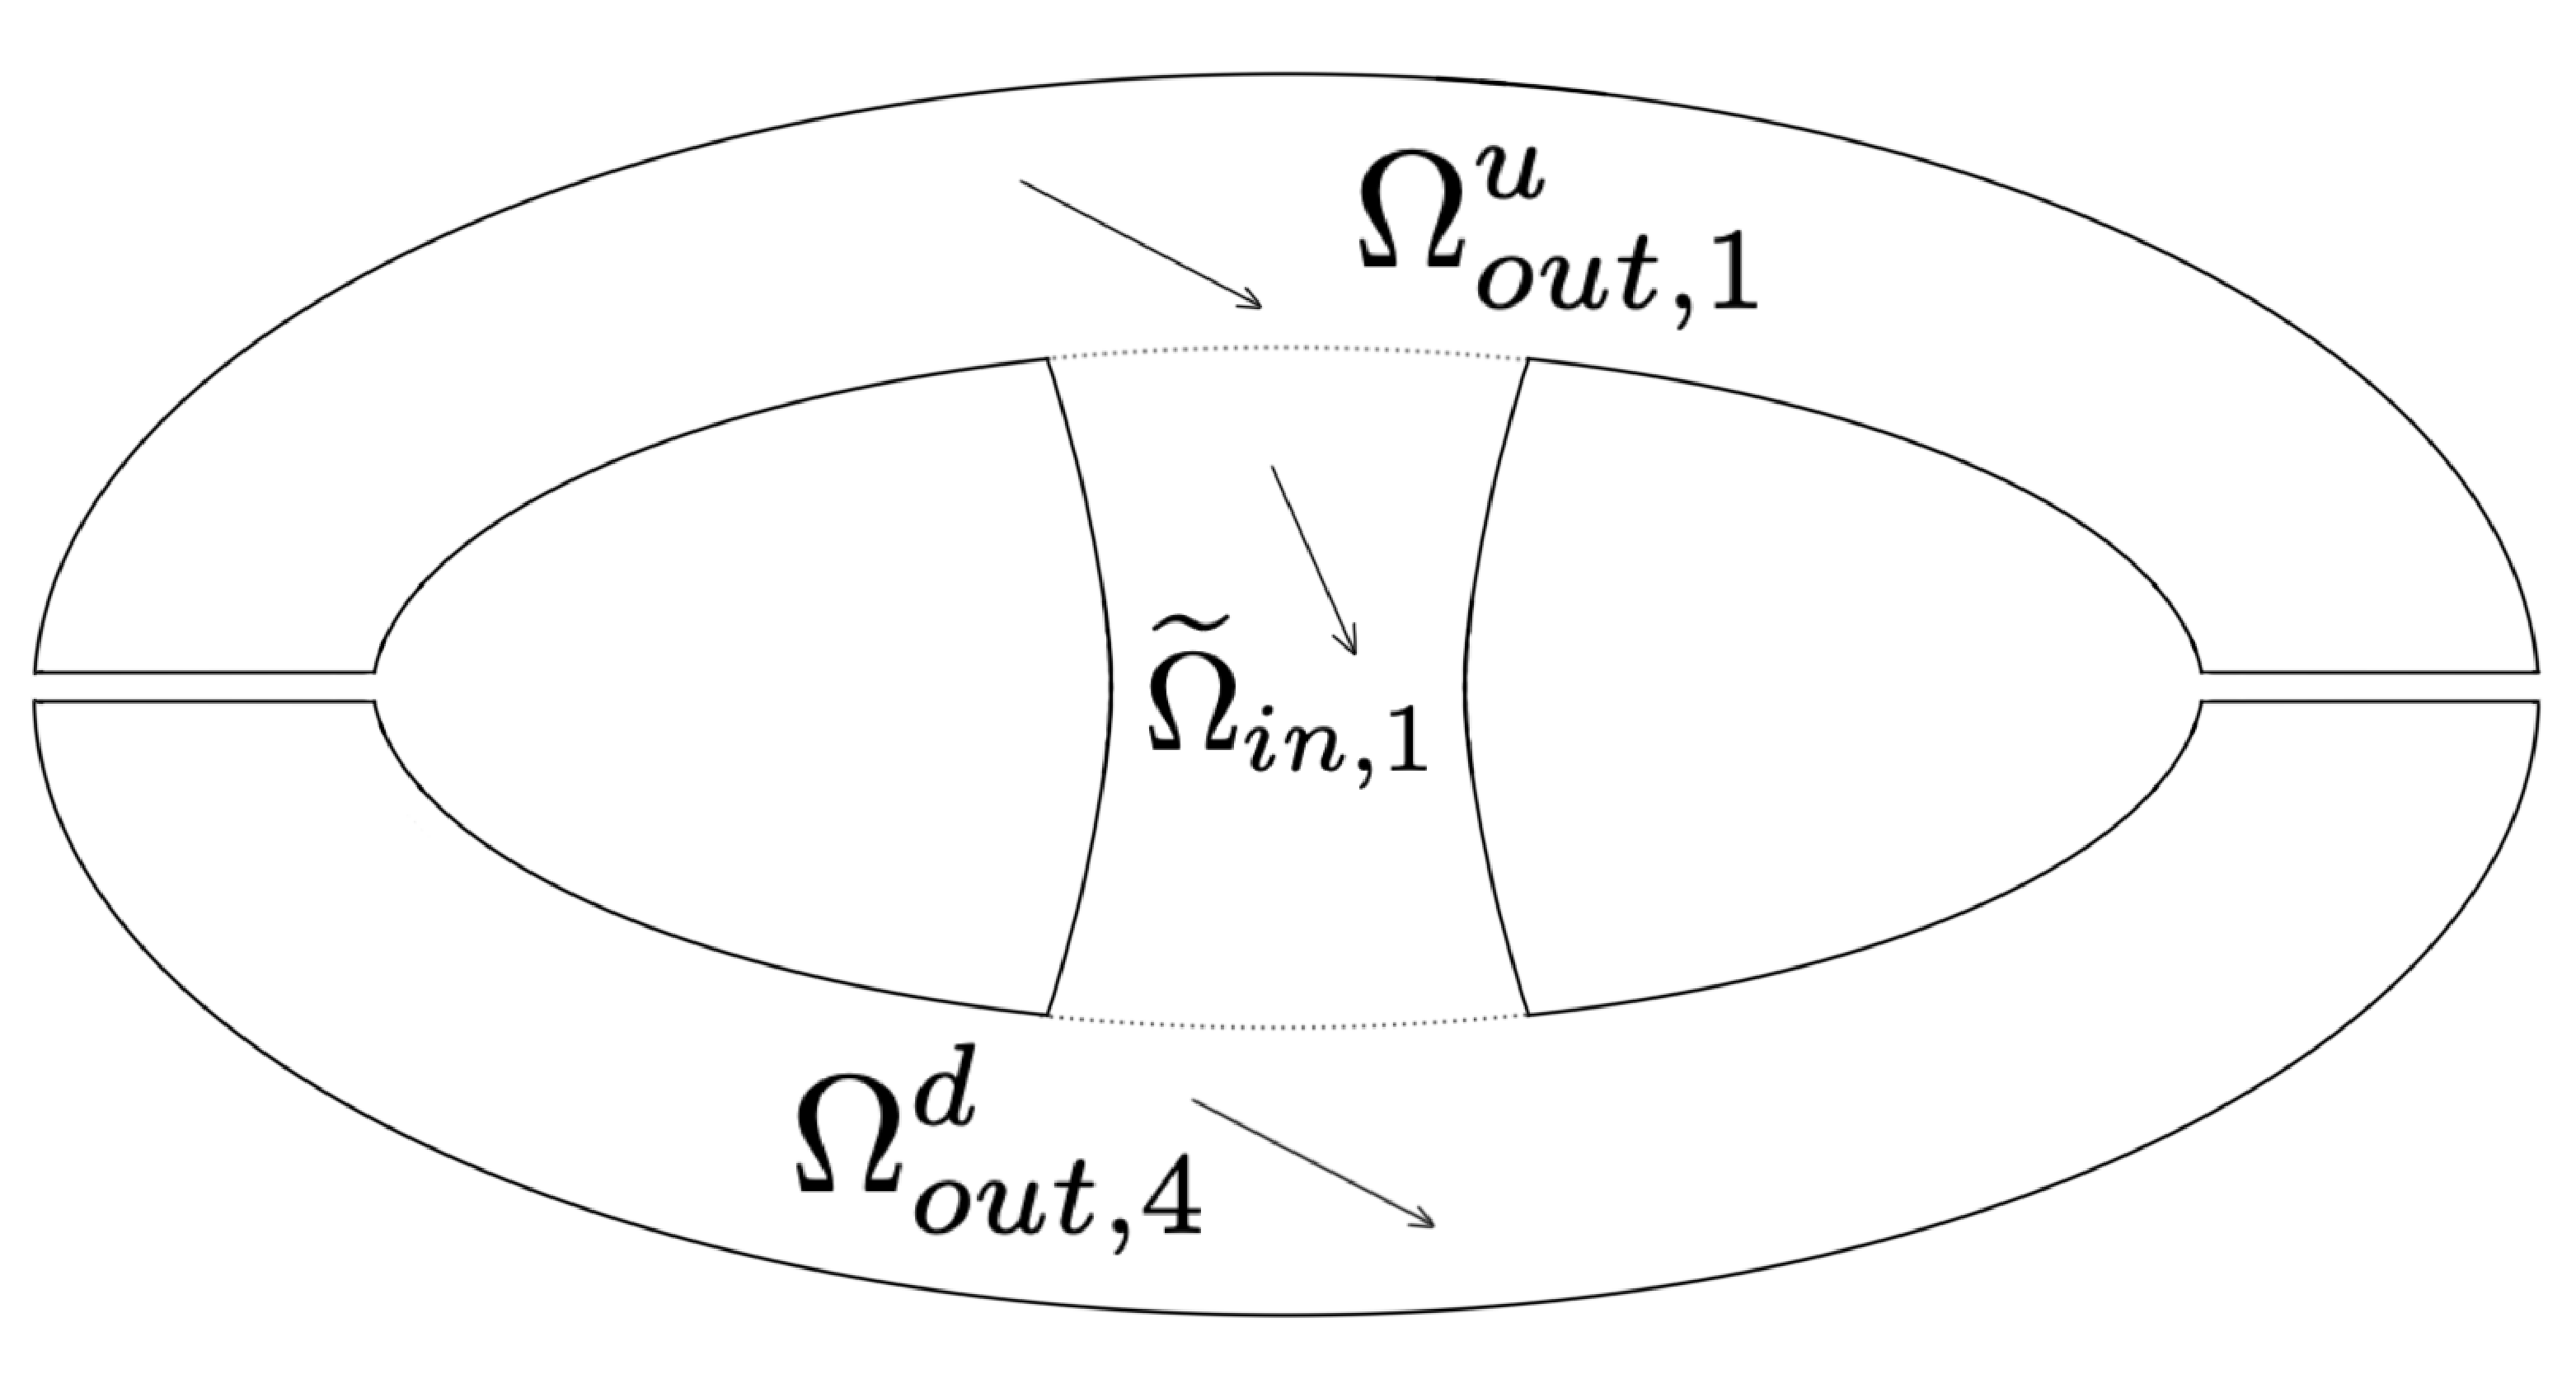
\includegraphics[scale=0.1]{images/section2/atoms/atom_5_domain.pdf}
    \caption{Пример области $\widetilde{\Omega}_1$ для перестройки 5.}
    \label{fig:pt9:_domain_atom_hyp_foc}
\endminipage\hfill
\minipage{0.5\textwidth}
\centering
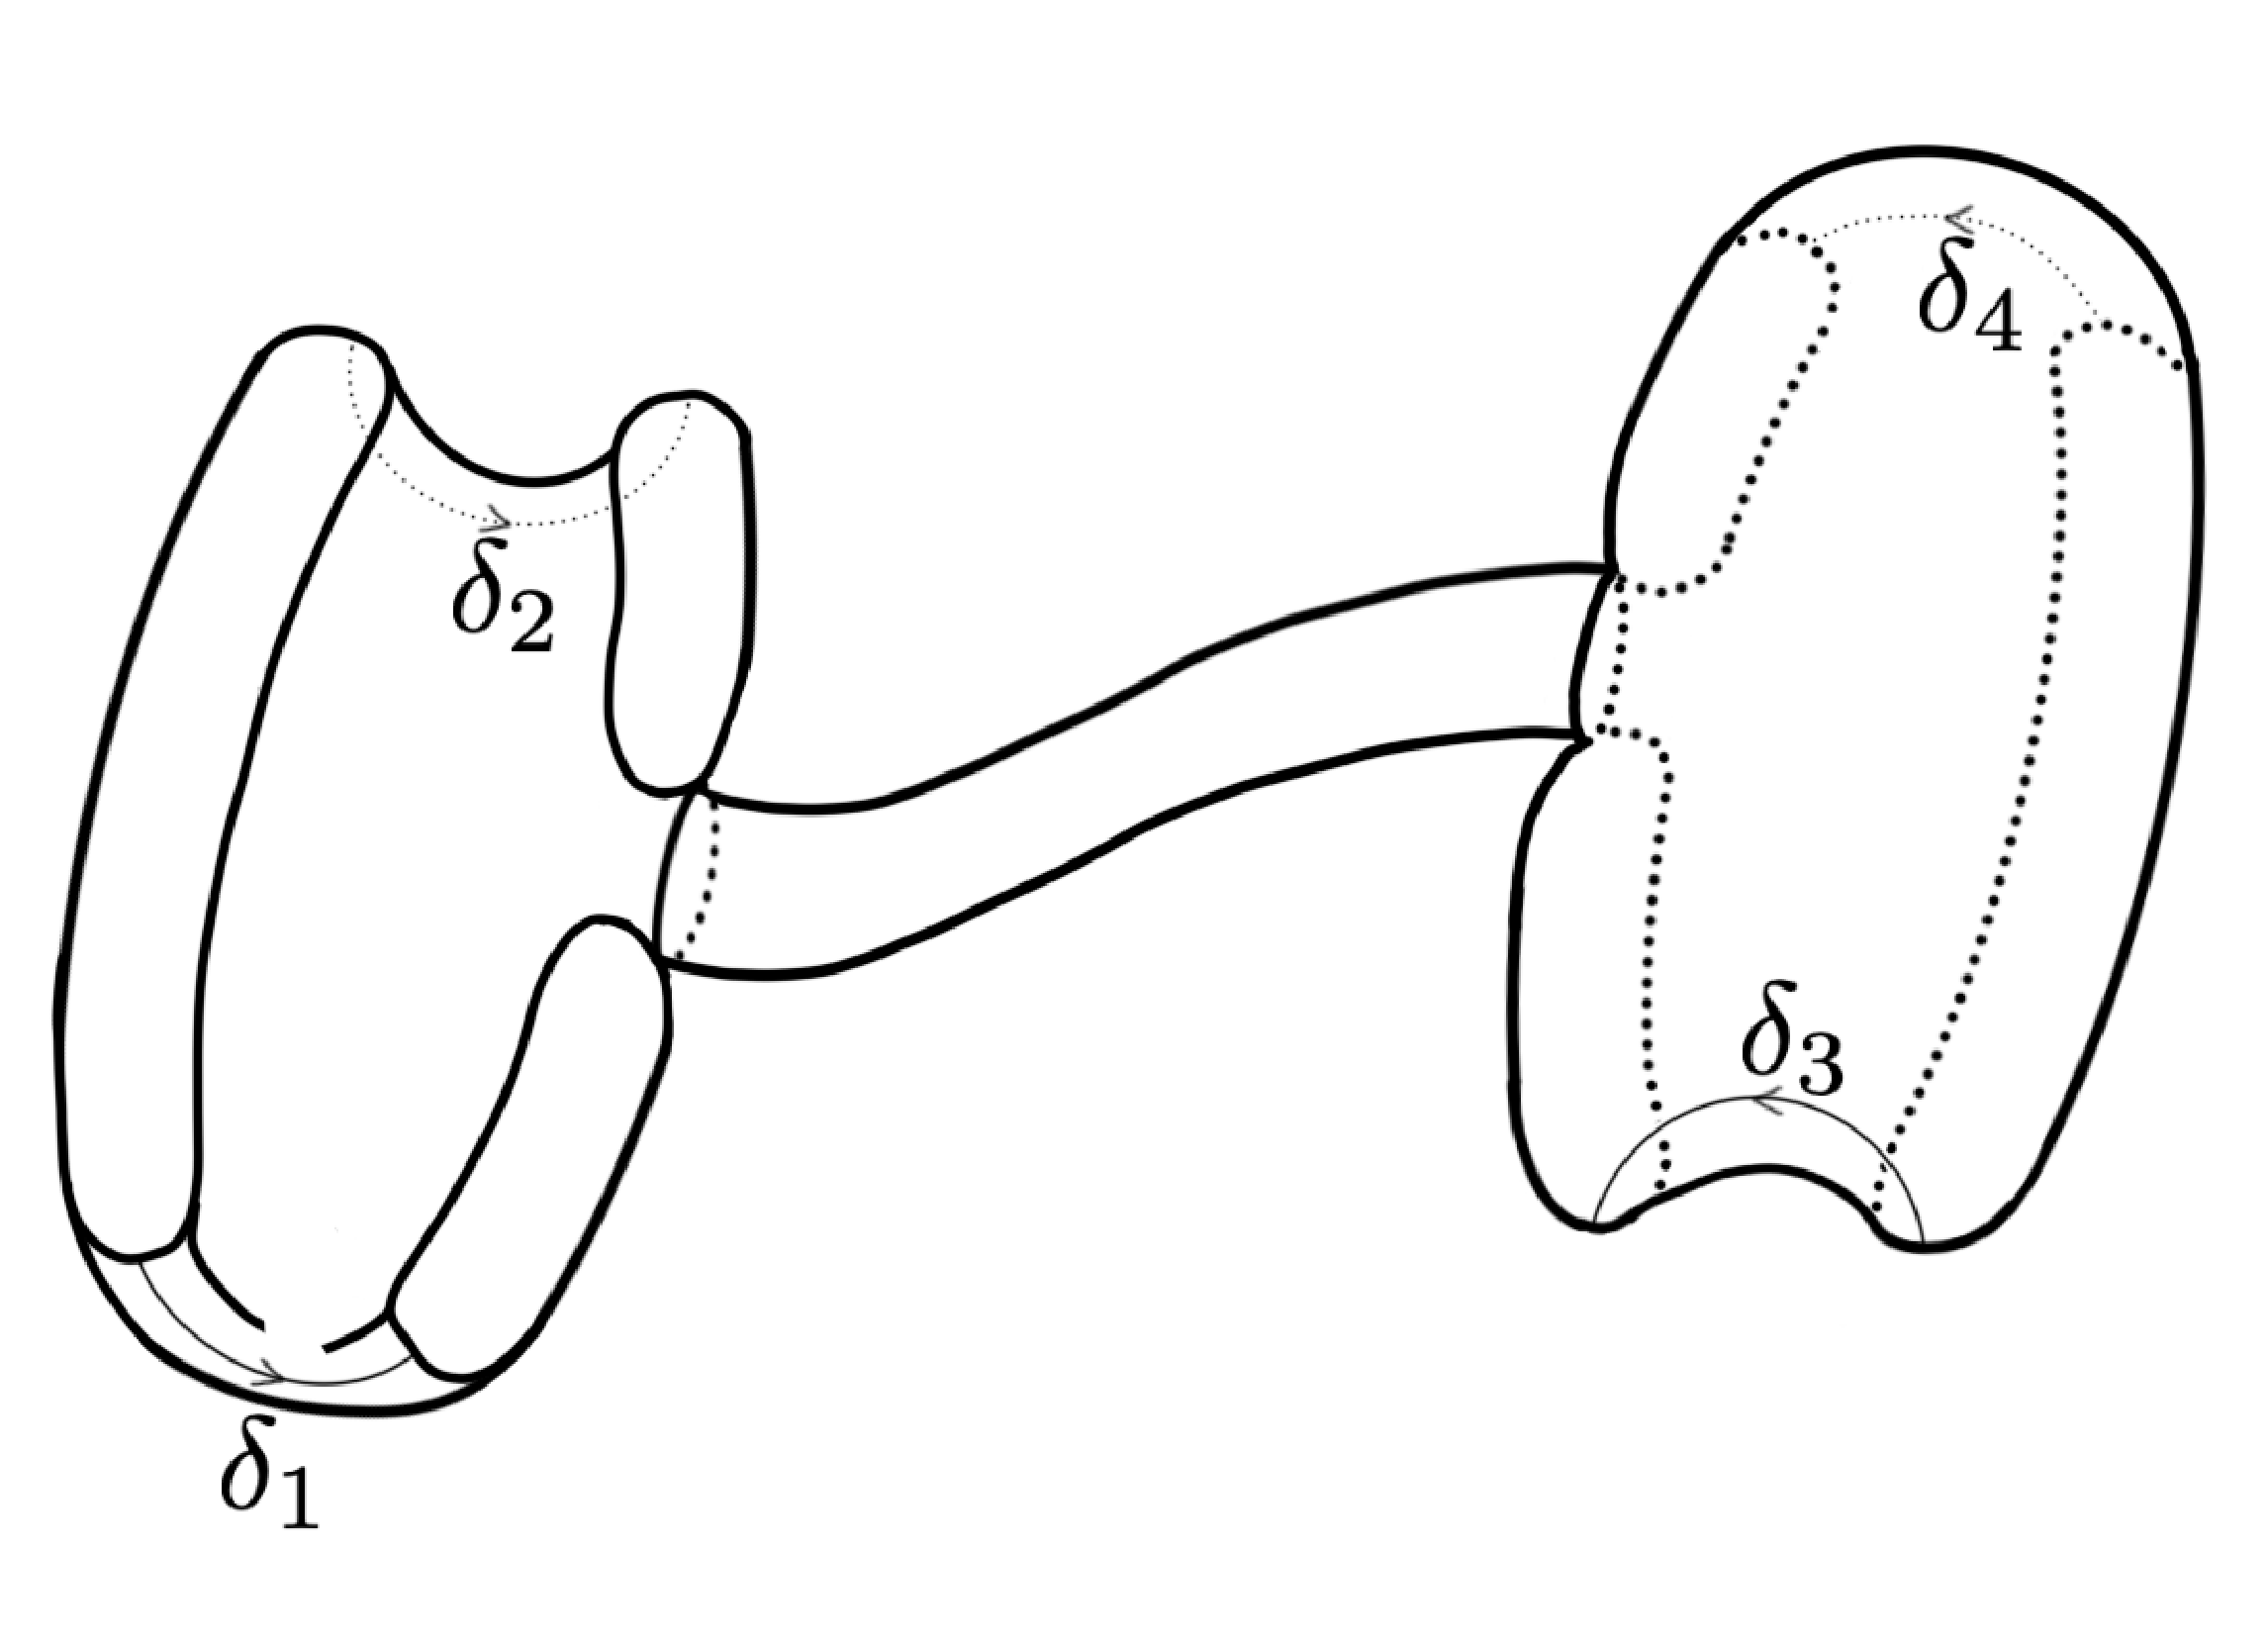
\includegraphics[scale=0.12]{images/section2/atoms/atom_5_half.pdf}
    \caption{Результат склейки $\widetilde{\Omega}_1 \cup \widetilde{\Omega}_2$ для перестройки 5.}
    \label{fig:pt9:_atom_5_half}
\endminipage\hfill
\end{figure}

Области $\widetilde{\Omega}_1$ и $\widetilde{\Omega}_2$ склеиваются по общим дугам на поверхности $\Xi = \const$, которые проектируются на граничные гиперболические дуги области $\widetilde{\Omega}$. Аналогично для областей $\widetilde{\Omega}_3$ и $\widetilde{\Omega}_4$. 
Те же пары областей также склеиваются по дугам, которые проектируются на горизонтальные отрезки $\Omega_{out} \cap \{y=0\}$. А именно, прообраз каждого из этих отрезков на поверхности $\Xi = \const$ эквивалентен окружности, половина дуги которого является общей границей областей $\Omega_{out, 1}^u, \Omega_{out, 2}^u, \Omega_{out, 1}^d, \Omega_{out, 2}^d$, а вторая половина дуги --- общая граница для областей $\Omega_{out, 3}^u, \Omega_{out, 4}^u, \Omega_{out, 3}^d, \Omega_{out, 4}^d$. 

Тогда склейка областей $\widetilde{\Omega}_1$ и $\widetilde{\Omega}_2$ по общим граничным дугам приводит к поверхности, изображенной на рис. \ref{fig:pt9:_atom_5_half}, край которой состоит из шести окружностей, которые проецируются на эллиптические граничные дуги области $\widetilde{\Omega}$ (см. рис. \ref{fig:pt9:_domain_atom_hyp_foc}). На склейке отметим дуги  $\delta_1, \ldots, \delta_4$, которые проецируются на горизонтальные отрезки $\Omega_{out} \cap \{y=0\}$.
Склейка областей $\widetilde{\Omega}_3 \cup \widetilde{\Omega}_4$ устроена аналогично. 

Для получения поверхности $\Xi = \const$ остается склеить $\widetilde{\Omega}_1 \cup \widetilde{\Omega}_2$ и $\widetilde{\Omega}_3 \cup \widetilde{\Omega}_4$ по общим граничным дугам, а также вдоль дуг $\delta_1, \ldots, \delta_4$. Поверхность $\Xi = \const$ до отождествления вдоль  $\delta_1, \ldots, \delta_4$ изображена на рис. \ref{fig:pt9:_atom_5}.

\begin{figure}[!htb]
\centering
\includegraphics[scale=0.125]{images/section2/atoms/atom_5.pdf}
    \caption{Поверхность уровня $\Xi = \const$ для перестройки 5.}
    \label{fig:pt9:_atom_5}
\end{figure}


%На Рис. \ref{fig:pt9:_hyp_foc_atom} изображена поверхность для особого значения интеграла.
%Пунктирами изображены сечения <<ручек>>.
%\begin{figure}[!htb]
%\centering
%\includegraphics[scale=0.15]{images/section2/atoms/hyp_foc_atom.pdf}
%    \caption{Результирующая поверхность для особого значения $\Lambda=b^2 n_{out}^2$.}
%    \label{fig:pt9:_hyp_foc_atom}
%\end{figure}

\textbf{Перестройка 6.} 
Продолжения звеньев траектории, находящихся в области $\Omega_{out}$ касаются эллипса с параметром $\alpha_{out}$, а в области $\Omega_{in}$ сегменты траектории совпадают с вертикальной полуосью эллипса.

Поверхность $\Xi = \const$ можно представлять себе как предельный случай неособой поверхности, соответствующей случаю $D_1^6$, при $\alpha_{in} \to a^2$ (см. рис. \ref{fig:pt9:_diagramPlusIrregular}), когда две ручки схлопываются в две дуги, причем имеющие общие концы. 

Напомним рассуждения, проведенные нами для случая $D_1^6$. Рассмотрим склейку областей $\widetilde{\Omega}_1$ (см. рис. \ref{fig:pt9:_ell_and_hyp_2}) и $\widetilde{\Omega}_3$ (см. рис. \ref{fig:pt9:_ell_and_hyp2_permutations}) и аналогичную склейку областей $\widetilde{\Omega}_2$ и $\widetilde{\Omega}_4$.
Затем $\widetilde{\Omega}_1 \cup \widetilde{\Omega}_3$ и $\widetilde{\Omega}_2 \cup \widetilde{\Omega}_4$ склеиваются по тем граничным дугам, которые проецируются в эллиптические граничные дуги области $\widetilde{\Omega}$. Результатом склейки являются два тора, соединенные лентами (см. рис.  \ref{fig:pt9:_ell_and_hyp2_transformations}). Каждая лента ограничивается дугами, которые проецируются в граничные гиперболические дуги области $\widetilde{\Omega}$. 
%Граничные дуги ленты на листе $\widetilde{\Omega}_1$ отождествляются с одноименными дугами ленты $\widetilde{\Omega}_2$, результатом является цилиндр. Граничные окружности этого цилиндра проецируются в область $\widetilde{\Omega}$ в дуги эллипса с параметром $\lambda_1$, находящиеся между ветвями гиперболы с параметром $\alpha_{in}$. Аналогично для областей $\widetilde{\Omega}_3$ и $\widetilde{\Omega}_4$. 
%При устремлении параметра $\alpha_{in}$ к $a^2$ ширина всех четырех лент устремляется к нулю, то есть ручка, полученная склейкой области $\widetilde{\Omega}_1$ с $\widetilde{\Omega}_2$ превращается в кривую, которая соединяет верхнюю и нижнюю вершины эллипса с параметром $\lambda_1$. Аналогично для областей $\widetilde{\Omega}_3$ и $\widetilde{\Omega}_4$.
%Поверхность уровня $\Xi = \const$ изображена на рис. \ref{fig:pt9:_atom_6} и представляет собой два тора, соприкасающихся по двум соединенным окружностью точкам.
Области $\widetilde{\Omega}_1$ и $\widetilde{\Omega}_2$ отождествляются по общим границам, проектирующимся на левую и правую ветви гиперболы $Q_{\alpha_{in}}$ в области $\Omega_{in}$. 

В момент перестройки ручка, образованная склейкой областей $\widetilde{\Omega}_1$ и $\widetilde{\Omega}_2$ (соответственно, $\widetilde{\Omega}_3$ и $\widetilde{\Omega}_4$) стягивается в кривую. 
То есть поверхность $\Xi = \const$ представляет собой два касающихся в двух точках тора, при этом обе общие точки этих двух торов соединены двумя кривыми, см. рис. \ref{fig:pt9:_atom_6}.
\begin{figure}[!htb]
\centering
\includegraphics[scale=0.09]{images/section2/atoms/atom_6.pdf}
    \caption{Поверхность уровня $\Xi = \const$ для перестройки 6.}
    \label{fig:pt9:_atom_6}
\end{figure}


\textbf{Перестройка 7.}
Сегменты бильярдной траектории в области $\Omega_{in}$ лежат на проходящих через фокусы прямых, не заходя при этом в область $\Omega_{out}$.

Положим $\widetilde{\Omega} = \Omega_{in}$. Проекция $\pi$ четырехлистна в любой внутренней точке $\widetilde{\Omega} \setminus \{y=0\}  = (\Omega_{in} \cap \{y>0\}) \cup (\Omega_{in} \cap \{y<0\}) = \Omega_{in}^u \cup \Omega_{in}^d$.
Тогда последние две области имеют на поверхности $\Xi = \const$ по четыре прообраза $\Omega_{in, j}^u, \Omega_{in, j}^d, j=1, \ldots, 4$, которые занумерованы в соответствии с правилом \eqref{eq:foc_numeration}.

На поверхности $\Xi = \const$ общая граничная дуга областей $\Omega_{in, 1}^u, \Omega_{in, 4}^u$ проецируется на дугу эллипса с параметром $\lambda_1$ в верхней полуплоскости. Аналогично для областей $\Omega_{in, 2}^u, \Omega_{in, 3}^u$. На симметричную дугу эллипса с параметром $\lambda_1$ проецируются граничные дуги для $\Omega_{in, 1}^d$ и $\Omega_{in, 4}^d$, аналогично для областей $\Omega_{in, 2}^d, \Omega_{in, 3}^d$. 
В соединяющий фокусы отрезок горизонтальной прямой проецируются общие граничные дуги областей $\Omega_{in, 1}^u, \Omega_{in, 4}^u, \Omega_{in, 1}^d, \Omega_{in, 4}^d$. Аналогично для областей $\Omega_{in, 2}^u, \Omega_{in, 3}^u, \Omega_{in, 2}^d$ и $\Omega_{in, 3}^d$.

Определим области 
\begin{equation}
\begin{array}{cc}
\widetilde{\Omega}_1 = \Omega_{in, 1}^u \cup \Omega_{in, 4}^d, &
\widetilde{\Omega}_2 = \Omega_{in, 2}^u \cup \Omega_{in, 3}^d, \\
\widetilde{\Omega}_3 = \Omega_{in, 3}^u \cup \Omega_{in, 2}^d, &
\widetilde{\Omega}_4 = \Omega_{in, 4}^u \cup \Omega_{in, 1}^d.
\end{array}
\label{eq:case7Omegas}
\end{equation}

Склеим области $\widetilde{\Omega}_1$ и $\widetilde{\Omega}_4$ по общим граничным областям, которые проецируются на эллиптические граничные дуги области $\widetilde{\Omega}$, а также по общей дуге, которая проецируется на соединяющие фокусы отрезок.
Аналогично склеим области $\widetilde{\Omega}_2$ и $\widetilde{\Omega}_3$. Результатами склеек являются два цилиндра с восьмерками в поперечных сечениях каждого.

Окружности, ограничивающие восьмерки на левом и правом торцах цилиндров, проецируются в левый и правый отрезки $\Omega_{in} \cap \{y=0\}$.
На этих отрезках отождествляются области $\Omega_{in, 1}^u$ и $\Omega_{in, 2}^d$. Аналогично для областей $\Omega_{in, 2}^u$ и $\Omega_{in, 1}^d$, для $\Omega_{in, 3}^u$ и $\Omega_{in, 4}^d$, а также $\Omega_{in, 4}^u$ и $\Omega_{in, 3}^d$.
Тогда на правом отрезке $\Omega_{in} \cap \{y=0\}$ \textit{верхняя} граничная окружность склейки $\widetilde{\Omega}_1 \cup \widetilde{\Omega}_4$ склеивается с  \textit{нижней} граничной окружностью склейки $\widetilde{\Omega}_2 \cup \widetilde{\Omega}_3$, а \textit{нижняя} окружность на  $\widetilde{\Omega}_1 \cup \widetilde{\Omega}_4$ --- с \textit{верхней} на $\widetilde{\Omega}_2 \cup \widetilde{\Omega}_3$. Аналогично на левом отрезке $\Omega_{in} \cap \{y=0\}$.

Таким образом, два цилиндра с восьмерками в сечении склеиваются в один тор с восьмеркой в сечении, образуя поверхность $\Xi = \const$.

\textbf{Перестройка 8.} 
Звенья траектории в области $\Omega_{in}$ касаются гиперболы с параметром $\alpha_{in}$, а в области $\Omega_{out}$ совпадают вертикальной полуосью граничного эллипса.

Поверхность $\Xi = \const$ можно представлять себе как предельный случай неособой поверхности, соответствующей случаю $D_1^2$, при $\alpha_{out} \to a^2$ (см. рис. \ref{fig:pt9:_diagramPlusIrregular}), когда две ручки схлопываются в окружности.

Напомним рассуждения, проведенные нами для случая $D_1^2$. Рассмотрим склейку областей $\widetilde{\Omega}_1$ (см.  рис. \ref{fig:pt9:_img17}) и $\widetilde{\Omega}_4$  по общим границам, которые проецируются в эллиптические граничные дуги области $\widetilde{\Omega}$ и аналогичную склейку областей $\widetilde{\Omega}_2$ и $\widetilde{\Omega}_3$.
Результатом склейки является сфера с шестью дырками, при этом каждая дырка ограничивается парой дуг на поверхности $\Xi=\const$, которые проецируются в граничные гиперболические дуги области $\widetilde{\Omega}$. 
Части границ областей $\widetilde{\Omega}_1$ и $\widetilde{\Omega}_2$ отождествляются по дугам, которые проектируются в часть границы области $\widetilde{\Omega}$, аналогично для областей $\widetilde{\Omega}_3$ и $\widetilde{\Omega}_4$.

На рис. \ref{fig:pt9:_atom_8_step} изображен результат склейки $\widetilde{\Omega}_1 \cup \widetilde{\Omega}_4$. Его границей являются три пары окружностей, по которым приклеивается поверхность, полученная в результате аналогичной склейки $\widetilde{\Omega}_2 \cup \widetilde{\Omega}_3$. 

В момент перестройки две верхние (соответственно, две нижние) граничные окружности $\widetilde{\Omega}_1 \cup \widetilde{\Omega}_4$ схлопываются в одну окружность. 

Таким образом, поверхность $\Xi = \const$ представляет собой тор, на котором отмечены две пары отождествленных точек, при этом из точек, полученных в результате отождествления, <<растет>> по одной окружности, см. рис. \ref{fig:pt9:_atom_8}.

%\begin{figure}[!htb]
%\minipage{0.33\textwidth}
%\centering
%\includegraphics[scale=0.07]{images/section2/atoms/domain_atom_hyp_void.pdf}
%    \caption{Соответствующая случаю 8 область $\Omega$.}
%    \label{fig:pt9:_domain_atom_hyp_void}
%\endminipage\hfill
%\minipage{0.32\textwidth}
%\centering
%\includegraphics[scale=0.07]{images/section2/atoms/domain_atom_hyp_void_before_limit.pdf}
%    \caption{Область $\Omega$ как предельный случай.}
%    \label{fig:pt9:_domain_atom_hyp_void_before_limit}
%\endminipage\hfill
%\minipage{0.3\textwidth}
%\centering
%\includegraphics[scale=0.1]{images/section2/atoms/atom_hyp_void_iter1.pdf}
%    \caption{Схлопывание одной из ручек.}
%    \label{fig:pt9:_atom_hyp_void_iter1}
%\endminipage\hfill
%\end{figure}
%
%Для того, чтобы получить сам атом, остается провести склейку как показано на Рис. \ref{fig:pt9:_atom_hyp_void_iter2}, результат которой можно увидеть на Рис. \ref{fig:pt9:_hyp_void_atom}.
%
\begin{figure}[!htb]
\minipage{0.5\textwidth}
\centering
\includegraphics[width=2.5cm]{images/section2/atoms/atom_8_step.pdf}
    \caption{Результат склейки $\widetilde{\Omega}_1 \cup \widetilde{\Omega}_4$ для перестройки 8.}
    \label{fig:pt9:_atom_8_step}
\endminipage\hfill
\minipage{0.5\textwidth}
\centering
\includegraphics[width=6cm]{images/section2/atoms/atom_8.pdf}
    \caption{Поверхность уровня $\Xi = \const$ для случая 8.}
    \label{fig:pt9:_atom_8}
\endminipage\hfill
\end{figure}


\textbf{Перестройка 9.}
Звенья траектории в области $\Omega_{out}$ лежат на касательных к гиперболе с параметром $\alpha_{out}$, а в области $\Omega_{in}$ совпадают с вертикальной полуосью эллипса.

Поверхность $\Xi = \const$ можно представить себе как предельный случай неособой поверхности, соответствующей случаю $D_1^3$, при $\alpha_{in} \to a^2$ (см. рис. \ref{fig:pt9:_diagramPlusIrregular}), когда две ручки схлопываются в окружность.

Напомним рассуждения случая $D_1^3$. Рассмотрим склейку областей  $\widetilde{\Omega}_1$ (см. рис. \ref{fig:pt9:_img18}) и $\widetilde{\Omega}_4$  по общим границам, которые проецируются в эллиптические граничные дуги области $\widetilde{\Omega}$ и аналогичную склейку для областей $\widetilde{\Omega}_2$ и $\widetilde{\Omega}_3$.
Результатом склейки является сфера с шестью дырками, при этом каждая дырка ограничивается парой дуг на поверхности $\Xi=\const$, которые проецируются в граничные гиперболические дуги области $\widetilde{\Omega}$. 

Части границ областей $\widetilde{\Omega}_1$ и $\widetilde{\Omega}_2$ отождествляются по дугам, которые проектируются в гиперболические дуги области $\widetilde{\Omega}$, аналогично для областей $\widetilde{\Omega}_3$ и $\widetilde{\Omega}_4$.

На рис. \ref{fig:pt9:_atom_9_step} изображен результат склейки $\widetilde{\Omega}_1 \cup \widetilde{\Omega}_4$. Границей этой поверхности являются три пары окружностей, по которым приклеивается поверхность, полученная в результате аналогичной  склейки  $\widetilde{\Omega}_2 \cup \widetilde{\Omega}_3$. 

В момент перестройки две граничные окружности $\widetilde{\Omega}_1 \cup \widetilde{\Omega}_4$, которые проецируются в область $\Omega_{in}$, стягиваются в одну окружность.

Таким образом, поверхность $\Xi = \const$ представляет собой два тора, на каждом из которых отождествлено по две точки. При этом точки, полученные в результате такого отождествления, соединены двумя дугами, см. рис. \ref{fig:pt9:_atom_9}.
%
%\begin{figure}[!htb]
%\minipage{0.33\textwidth}
%\centering
%\includegraphics[scale=0.1]{images/section2/atoms/domain_atom_void_hyp.pdf}
%    \caption{Соответствующая случаю область $\Omega$.}
%    \label{fig:pt9:_domain_atom_void_hyp}
%\endminipage\hfill
%\minipage{0.32\textwidth}
%\centering
%\includegraphics[scale=0.1]{images/section2/atoms/domain_atom_void_hyp_before_limit.pdf}
%    \caption{Область $\Omega$ как предельный случай.}
%    \label{fig:pt9:_domain_atom_void_hyp_before_limit}
%\endminipage\hfill
%\minipage{0.3\textwidth}
%\centering
%\includegraphics[scale=0.2]{images/section2/atoms/atom_void_hyp_iter1.pdf}
%    \caption{Схлопывание одной из ручек.}
%    \label{fig:pt9:_atom_void_hyp_iter1}
%\endminipage\hfill
%\end{figure}
%
%Для того, чтобы получить сам атом, остается провести склейку как показано на Рис. \ref{fig:pt9:_atom_void_hyp_iter2}, результат которой можно увидеть на Рис. \ref{fig:pt9:_void_hyp_atom}.

\begin{figure}[!htb]
\minipage{0.5\textwidth}
\centering
\includegraphics[width=2.5cm]{images/section2/atoms/atom_9_step.pdf}
\caption{Результат склейки $\widetilde{\Omega}_1 \cup \widetilde{\Omega}_4$ для перестройки 9.}
\label{fig:pt9:_atom_9_step}
\endminipage\hfill
\minipage{0.5\textwidth}
\centering
\includegraphics[width=5cm]{images/section2/atoms/atom_9.pdf}
\caption{Поверхность $\Xi = \const$ для случая 9.}
\label{fig:pt9:_atom_9}
\endminipage\hfill
\end{figure}

\textbf{Перестройка 10.}
Эта перестройка совпадает с перестройкой $\alpha_{out} \to b^2$ классического бильярда в эллиптическом кольце $\Omega_{out}$. Перестройка подробно разобрана в \cite[\S 3]{Fok15}.

\textbf{Перестройка 11.}
Как было отмечено выше, прямая \eqref{eq:L_line} проходит через точку $(\alpha_{in}, \alpha_{out}) = (\lambda_1, \lambda_1)$ и имеет коэффициент наклона $\dfrac{n_{in}^2}{n_{out}^2}$. 
Следовательно, такая перестройка возможна лишь в случае $n_{in}^2 = n_{out}^2$, что соответствует отсутствию преломления. Такая перестройка рассматривается в теории классического бильярда, см. \cite[\S 3]{Fok15}.

\textbf{Перестройка 12.}
Звенья траектории в области $\Omega_{in}$ лежат на проходящих через фокусы прямых, а в области $\Omega_{out}$ совпадают с вертикальной полуосью эллипса. 

Поверхность $\Xi = \const$ можно представить себе как комбинацию перестроек $\textbf{4}$ и $\textbf{8}$ (или перестроек $\textbf{3}$ и $\textbf{7}$). 

Определим области $\widetilde{\Omega}_1, \ldots, \widetilde{\Omega}_4$, как в \eqref{fig:pt9:_atom_4_domain} (пример области см. рис. \ref{fig:pt9:_atom_4_domain}).
Склеим листы $\widetilde{\Omega}_1$ и  $\widetilde{\Omega}_4$ так же, как указано в \textbf{перестройке 4}. В момент перестройки граничные окружности должны схлопнуться в одну окружность. Поэтому те части склейки, которые проецируются в кольцо $\Omega_{out}$, продеформируем так же, как в \textbf{перестройке 8} (результат склейки см. рис. \ref{fig:pt9:_atom_12_half}).

Таким образом, поверхность $\Xi = \const$ представляет собой тор с восьмеркой в сечении, на котором отмечены  две пары отождествленных точек, принадлежащих разным <<компонентам>> восьмерок. При этом из точек, полученных в результате отождествления, <<растет>> по одной окружности, см. рис. \ref{fig:pt9:_atom_12}.


\begin{figure}[!htb]
\minipage{0.5\textwidth}
\centering
\includegraphics[scale=0.3]{images/section2/atoms/atom_12_half.pdf}
    \caption{Схема склейки $\Omega_1 \cup \Omega_4$ и $\Omega_2 \cup \Omega_3$ для случая 12.}
    \label{fig:pt9:_atom_12_half}
\endminipage\hfill
\minipage{0.5\textwidth}
\centering
\includegraphics[scale=0.2]{images/section2/atoms/atom_12.pdf}
    \caption{Поверхность уровня $\Xi = \const$ для случая 12.}
    \label{fig:pt9:_atom_12}
\endminipage\hfill
\end{figure}



\textbf{Перестройка 13.}
Звенья траектории в области $\Omega_{out}$ лежат на проходящих через фокусы прямых, а в области $\Omega_{in}$ совпадают с вертикальной полуосью эллипса.

Поверхность $\Xi = \const$ можно представить себе как комбинацию перестроек $\textbf{5}$ и $\textbf{9}$ (или перестроек $\textbf{6}$ и $\textbf{10}$).

Определим области $\widetilde{\Omega}_1, \ldots, \widetilde{\Omega}_4$, как в \eqref{eq:case5Omegas} (пример области см. рис. \ref{fig:pt9:_domain_atom_hyp_foc}).
Склеим листы $\widetilde{\Omega}_1$ и  $\widetilde{\Omega}_4$ так же, как указано в \textbf{перестройке 5}. В момент перестройки две трубки, образованные проецирующимися в $\Omega_{in}$ частями листов, должны схлопнуться в одну окружность. Отождествим полученную поверхность вдоль дуг $\delta_1, \ldots, \delta_4$, результат склейки изображен на  рис. \ref{fig:pt9:_atom_13_half}.

Поверхность $\Xi = \const$ получается склейкой поверхности по граничным окружностям, результат изображен на рис. \ref{fig:pt9:_atom_13}.

\begin{figure}[!htb]
\minipage{0.5\textwidth}
\centering
\includegraphics[scale=0.1]{images/section2/atoms/atom_13_half.pdf}
    \caption{Схема склейки $\Omega_1 \cup \Omega_2$ и $\Omega_3 \cup \Omega_4$ для случая 13.}
    \label{fig:pt9:_atom_13_half}
\endminipage\hfill
\minipage{0.5\textwidth}
\centering
\includegraphics[scale=0.1]{images/section2/atoms/atom_13.pdf}
    \caption{Поверхность уровня $\Xi = \const$ для случая 13.}
    \label{fig:pt9:_atom_13}
\endminipage\hfill
\end{figure}

           % Глава 9
\section{Задача Б.}\label{sec:ch4/sec3}
%\section{Случай с преломлением по двум пересекающимся в точке квадрикам}\label{s3}

\subsection{Постановка задачи}\label{sec:ch4/sec3/subsec1}
Пусть область $\Omega$ --- пересечение кольца $\{r_0^2 \leq x^2 + y^2 \leq r_2^2\}$ с правой полуплоскостью $\{x\geq 0\}$. Область $\Omega$ разбита на две части $\Omega_1$ и $\Omega_2$ дугой  $EF$ окружности радиуса $r_1$, где $r_0  < r_1 <r_2$ и сегментом  $FG$ горизонтального диаметра (см. рис. \ref{fig:pt10:_domain}). Зафиксируем показатели преломления: $n_1$ для области $\Omega_1$ и $n_2$ --- для  $\Omega_2$.
\begin{figure}[!htb]
\centering
\includegraphics[scale=0.3]{images/ch4/section3_circular/domain.pdf}
    \caption{Область $\Omega$ представляет собой объединение 2 областей.}
    \label{fig:pt10:_domain}
\end{figure}


В области $\Omega = \Omega_1 \cup \Omega_2$ рассмотрим бильярдную систему, подчиняющуюся закону $(\ast)$.
В предыдущем разделе была введена функция $\Lambda(x,y,v_x, v_y)$: ее значение равно параметру $\alpha$ софокусной квадрики $\frac{x^2}{a^2-\alpha} + \frac{y^2}{b^2-\alpha} = 1$, которой касается бильярдная траектория, проходящая через точку $(x,y)$ с вектором скорости $(v_x, v_y)$.
% А именно, в области $\Omega_i$ значение $\Lambda(x,y,v_x, v_y) = \alpha_i$ является параметром квадрики, которая задается уравнением $\frac{x^2}{a^2-\alpha_i} + \frac{y^2}{b^2-\alpha_i} = 1$. 
В частном случае, когда большая и малая полуоси $a$ и $b$ эллипса  совпадают, уравнение квадрики можно записать в виде $x^2 + y^2 = a^2-\alpha = \rho^2$, где $\rho$ --- радиус окружности, касающейся звена траектории.
Величина $\rho^2$ является функцией положения и скорости материальной точки и задается формулой $$\rho^2(x,y,v_x,v_y) = a^2 - \Lambda(x, y, v_x, v_y) = \frac{(x v_y - y v_x)^2}{v_x^2 + v_y^2}.$$
Для классического бильярда в круге  функция $\rho^2$ является первым интегралом, не зависящим от полной энергии.

\subsection{Интеграл $\rho^2$. Условия полного внутреннего отражения}\label{sec:ch4/sec3/subsec2}
Общая граница областей $\Omega_1$ и $\Omega_2$ состоит из двух кривых: из сегмента окружности $EF$ и отрезка прямой $FG$. 
Пусть материальная точка двигается с вектором скорости $(v_x, v_y)$ в области $\Omega_1$ и в точке с координатами $(x,y) \in EF \cup FG$ преломляется, после чего продолжает движение в области $\Omega_2$ с вектором скорости $(w_x, w_y)$. 

Проведем через точку $(x,y)$ прямую с вектором направления $(v_x, v_y)$: она касается некоторой окружности с центром в начале координат. Обозначим ее радиус через $\rho_1$. Аналогично $\rho_2$ определим как радиус окружности, касательной к проходящей через ту же точку $(x,y)$ прямой с вектором направления $(w_x, w_y)$.
Тогда в зависимости от того, к какой части общей границы областей $\Omega_1$ и $\Omega_2$  принадлежит точка $(x,y)$, величины $\rho_1^2$ и $\rho_2^2$ удовлетворяют одному из двух равенств. 
\begin{statement}
Имеют место следующие соотношения для параметров $\rho_1, \rho_2$ в точке преломления:
\begin{align}
(\rho_1^2 - r_1^2)n_1^2 = (\rho_2^2 - r_1^2)n_2^2 \qquad & 
			\text{ при } (x,y) \in EF, 
			\label{eq:st1_eq1}
			\\
\rho_1^2 n_1^2 = \rho_2^2 n_2^2 \qquad  & \text{ при } (x,y) \in FG.
			\label{eq:st1_eq2}
\end{align}
\label{st:across_EF}
\end{statement}
\begin{remark}
В доказательстве будут заодно отмечены условия, при которых бильярдная траектория преломляется и при которых испытывает полное  отражение.
\end{remark}

\begin{proof}
Пусть $(x,y) \in EF$, то есть траектория преломляется на дуге окружности с радиусом $r_1$. 
Угол $\theta_1$ откладывается между вектором скорости $(v_x, v_y)$ и вектором нормали окружности, который пропорционален радиус-вектору $(x,y)$. Тогда в обозначениях $\textbf{x}^2 = x^2+y^2$, $\textbf{v}^2=v_x^2+v_y^2$ рассмотрим величину
\begin{multline*}
\frac{r_1^2-\rho_1^2}{r_1^2} = \frac{1}{\textbf{x}^2} \left(\textbf{x}^2- \frac{(x v_y-y v_x)^2}{\textbf{v}^2}  \right) = \\
\frac{1}{\textbf{x}^2 \textbf{v}^2}\left( \textbf{x}^2 \textbf{v}^2 - (x^2 v_y^2 - 2xyv_xv_y+y^2v_x^2) \right) =
 \frac{1}{\textbf{x}^2\textbf{v}^2}\left( x^2 v_x^2 + 2xyv_xv_y+y^2v_y^2 \right) = \\
  \frac{1}{\textbf{x}^2\textbf{v}^2}(x v_x + y v_y)^2 = 
  \frac{1}{\textbf{x}^2\textbf{v}^2}\langle (x, y) , (v_x, v_y) \rangle^2 =
\cos^2 \theta_1,
\end{multline*}
где угол $\theta_1$ корректно определен при $\cos^2 \theta_1 \in (0,1)$, то есть косинус угла имеет смысл при $\rho_1^2 \in (0, r_1^2)$. 

Эта формула теряет смысл при $\rho_1 > r_1$ (когда бильярдная траектория не пересекает дугу $EF$) --- тогда $\cos^2 \theta_1 < 0$; случай $\cos^2 \theta_1 > 1$ соответствует $\rho_1^2 < 0$.
%Случай $\cos^2 \theta_1 <0$ соответствует $\rho_1 > r_1$, то есть дуга $EF$ и бильярдная траектория лежат по разные стороны от окружности радиуса $\rho_1$. 
%Неравенству $\cos^2 \theta_1 >1$ соответствует $\rho_1^2 <0$, что невозможно для вещественного радиуса $\rho_1$. 
Аналогичные соображения справедливы для $\cos^2 \theta_2 = \frac{r_1^2-\rho_2^2}{r_1^2}$.

Пусть $n_1 < n_2$. Тогда если величина $\frac{n_2}{n_1} \cos \theta_2 \in [-1,1]$, то в силу закона $(\ast)$ она совпадает с корректно определенным $\cos \theta_1$, откуда следует первое равенство утверждения. 
Остается лишь записать тождество  $(n_1 \cos \theta_1)^2 = (n_2 \cos \theta_2)^2$ через $r_1, \rho_1, \rho_2$, согласно приведенным выше выражениям.
При $\cos \theta_2 > \frac{n_1}{n_2}$ не существует удовлетворяющий закону преломления $\cos \theta_1$, и траектория отражается от $EF$ в область $\Omega_2$. 

Случай $n_1 > n_2$ рассматривается аналогично: величина $\frac{n_1}{n_2} \cos \theta_1 \in [-1,1]$, соответствует корректно определенному  $\cos \theta_2$, что позволяет получить нужное равенство. При $\cos \theta_1 > \frac{n_2}{n_1}$ траектория отражается от $EF$ в область $\Omega_1$. 


Пусть $(x,y) \in FG$, то есть траектория преломляется на отрезке горизонтальной прямой $\left\{ x \in (r_1,r_2), y=0 \right\}$. Тогда 
$$\frac{\rho_1^2}{x^2} = \frac{(x v_y-y v_x)^2}{x^2 \textbf{v}^2} = \frac{(x v_y)^2}{x^2 \textbf{v}^2} = \frac{v_y^2}{\textbf{v}^2} = \cos^2\theta_1, $$
аналогично получается равенство $\frac{\rho_2^2}{x^2} = \cos^2 \theta_2$. Из закона $(\ast)$ следует второе равенство утверждения везде, где корректно определены $\cos^2 \theta_1$ и $\cos^2 \theta_2$.
Опишем области корректного определения указанных величин.

Для первой координаты точки на сегменте $FG$ справедливо $x \in (r_1, r_2)$, следовательно $\frac{1}{x^2} \in (\frac{1}{r_2^2}, \frac{1}{r_1^2})$.
Косинус $\cos \theta_1$ корректно определен тогда и только тогда, когда $\frac{\rho_1^2}{x^2} \in (0,1)$, то есть $\frac{1}{x^2} \in (0,\frac{1}{\rho_1^2})$.
Комбинируя эти неравенства, выделим следующие случаи:

$\bullet$ При $\frac{1}{r_1^2} < \frac{1}{\rho_1^2}$ в каждой точке $FG$ определен $\cos \theta_1$;

$\bullet$ При $\frac{1}{r_2^2} < \frac{1}{\rho_1^2} < \frac{1}{r_1^2}$ в точках $x > \rho_1$ отрезка $FG$ определен $\cos \theta_1$;

$\bullet$ При $\frac{1}{\rho_1^2} < \frac{1}{r_2^2}$ ни в одной точке отрезка  $FG$ не определен $\cos \theta_1$.

Аналогично выделяются случаи, в которых определен $\cos \theta_2$. 
Таким образом, бильярдная траектория преломляется в любой точке $FG$ при $\max( \rho_1, \rho_2) < r_1$. При $r_1 < \max( \rho_1, \rho_2)$ траектория может преломиться в точках $(x,0) \in FG$, где $\max( \rho_1, \rho_2)  <x < r_2$. 

\end{proof}

\begin{remark}
Если траектория при переходе из $\Omega_1$ в $\Omega_2$ преломляется на дуге $EF$, то для величины $\rho_2^2$ справедливо $0 < \rho_2^2 < r_1^2$. 
И наоборот, если траектория при переходе из $\Omega_2$ в $\Omega_1$  преломляется на дуге $EF$, то для величины $\rho_1^2$ справедливо $0 < \rho_1^2 < r_1^2$. 
\label{cons:branching_zone_origins}
\end{remark}

Разобьем бильярдную траекторию в точках пересечения дуги $EF$ на фрагменты $T_k, k \geq 1$. 


%\textcolor{red}{=========== ниже плохое ===========}
% 
%Рассмотрим бильярдную траекторию, которая проходит из области $\Omega_1$ в область $\Omega_2$, пересекая отрезок $FG$, и возвращается в $\Omega_1$, пересекая дугу окружности $EF$. 
%Пусть радиус каустики до перехода через $FG$ равен $\rho_1$. 
%Из только что доказанного утверждения следует, что продолжения звеньев траектории после преломления на $FG$ касаются окружности радиуса $\rho_2$, где $\rho_2^2 = \rho_1^2 \frac{n_1^2}{n_2^2}$. 
%Если теперь траектория переходит через дугу $EF$, то после преломления звенья будут лежать на касательных прямых к окружности радиуса $\widetilde{\rho}_1 \neq \rho_1$, где $\widetilde{\rho}_1^2 = (\rho_2^2 - r_1^2)\frac{n_2^2}{n_1^2} + r_1^2$. 
%Подставим в полученное равенство выражение для $\rho_2^2$:
%\begin{equation}
%\widetilde{\rho}_1^2 = (\rho_2^2 - r_1^2)\frac{n_2^2}{n_1^2} + r_1^2 = \rho_1^2 +\frac{ r_1^2 (n_1^2 - n_2^2)}{n_1^2} = \rho_1^2 + \frac{\gamma}{n_1^2}, \ \gamma = r_1^2 (n_1^2-n_2^2),
%\label{eq:gammaDef}
%\end{equation}
%где коэффициент $\gamma$ не зависит от конкретного выбора траектории, которая проходит из области $\Omega_1$ в область $\Omega_2$, пересекая отрезок $FG$, и возвращается в $\Omega_1$, пересекая дугу окружности $EF$. 
%
%Предположим, что продолжение траектории <<обходит>> точку $F$ и снова пересекает отрезок $FG$. Тогда, повторяя вышеприведенные рассуждения для радиуса каустики $\widetilde{\rho}_2$ после второго преломления на отрезке $FG$, получим равенство $\widetilde{\rho}_2^2 = \rho_2^2 + \frac{\gamma}{n_2^2}$. 
%
%При обходе точки $F$ по часовой стрелке из параметров каустик $\rho_1^2$ и $\rho_2^2$ в областях $\Omega_1$ и $\Omega_2$ будут вычитаться  дроби $\frac{\gamma}{n_1^2}$ и $\frac{\gamma}{n_2^2}$, соответственно.
%
%Таким образом, на любой бильярдной траектории величина  $\rho_1^2$ в области $\Omega_1$ определена с точностью до добавления параметра $\frac{\gamma}{n_1^2}$, а $\rho_2^2$ в области $\Omega_2$ --- с точностью до добавления параметра $\frac{\gamma}{n_2^2}$. 
%
%\begin{remark}
%Обратим внимание на то, что на каждой траектории может появляться лишь конечное количество значений такого вида.
%
%Действительно, поскольку $\gamma$ (см. \eqref{eq:gammaDef}) не зависит от параметров траектории, то для произвольного $\rho_i < r_1$ начиная с некоторого $k$ выполняется $\rho_i + k \gamma > r_1$,  следовательно траектория не сможет пересечь дугу окружности $EF$. 
%
%Наоборот, для некоторого $m_0 > 0$ будет выполнено неравенство $\rho_i - m_0 \gamma < 0$. Тогда для всех $m\geq m_0$ выполнено $\rho_i - m \gamma  < 0$ и траектория отражается на ребре $EF$ или $FG$ в соответствии с законом $(\ast)$.
%\label{rem:finiteRevolutions}
%\end{remark}
%\textcolor{red}{=========== все ===========}

%Таким образом, в зависимости от того, по какому ребру траектория переходит из области $\Omega_1$ в область $\Omega_2$, радиус квадрики $\rho_2$ может быть определен одним из двух случаев. То есть, функция $\rho_2(\rho_1)$ является многозначной функцией. 

Каждый фрагмент бильярдной траектории $T_k$ образует ломаную кривую в $\Omega \setminus EF$, где $EF  \subset \partial \Omega_1 \cap \partial \Omega_2$.
Введем на $\Omega \setminus EF$ функцию $\Xi(x, y, v_x, v_y)$ по формуле
\begin{equation}
\Xi(x, y, v_x, v_y) = \left[
\begin{array}{ll}
    \rho^2(x,y,v_x,v_y) n_1^2, &  \text{ если } (x,y) \in \Omega_1 \\
    \rho^2(x,y,v_x,v_y) n_2^2, & \text{ если } (x,y) \in \Omega_2.
\end{array}
\right.
\label{eq:XiDefinition}
\end{equation}
Эта функция постоянна в каждой точке фрагмента бильярдной траектории $T_k$, но на разных фрагментах значения могут различаться. 

Рассмотрим значения интеграла $\Xi$ для двух последовательных фрагментов $T_k, T_{k+1}$. Выясним, как они связаны, или, что то же самое, как меняется интеграл $\Xi$ при преломлении на дуге $EF$. 

\begin{statement}
Значения $\Xi_k$ и $\Xi_{k+1}$  интеграла $\Xi$, соответствующие фрагментам траектории $T_k$ и $T_{k+1}$, различаются на величину $r_1^2(n_1^2-n_2^2)$.
\end{statement}
\begin{proof}
Значение $\Xi_k$ на фрагменте $T_k$ определяет радиусы $\rho_1$ и $\rho_2$ по формуле \eqref{eq:XiDefinition}. Здесь $\rho_1$ и $\rho_2$ являются радиусами окружностей, которых касаются звенья (или их продолжения) фрагмента $T_k$, содержащиеся в областях $\Omega_1$ и $\Omega_2$, соответственно.
Аналогично определяются радиусы $\widetilde{\rho}_1$ и $\widetilde{\rho}_2$ для фрагмента $T_{k+1}$ бильярдной траектории.
%касаются окружности радиуса $\rho_1$, а содержащиеся в $\Omega_2$ --- окружности радиуса $\rho_2$. Аналогично
%, которые определяют радиусы касательных окружностей к сегментам $T_k$


Пусть бильярдная траектория при преломлении на дуге $EF$ переходит из области $\Omega_1$ в область $\Omega_2$. 
%Обозначим радиус касательной к траектории окружности до преломления через $\rho_1$, а радиус аналогичной окружности после преломления в $\Omega_2$ --- через $\widetilde{\rho}_2$. 
Тогда радиусы $\rho_1^2$ и $\widetilde{\rho}_2^2$ связаны формулой \eqref{eq:st1_eq1}:  $(\rho_1^2 - r_1^2)n_1^2 = (\widetilde{\rho}_2^2 - r_1^2)n_2^2$.
С другой стороны, по формуле \eqref{eq:XiDefinition}: $\Xi_k = \rho_1^2 n_1^2$ и $\Xi_{k+1} = \widetilde{\rho}_2^2 n_2^2$.
Следовательно, $\Xi_k = \Xi_{k+1}  +r_1^2 (n_1^2 - n_2^2 )$.

Аналогично рассматривается случай, когда траектория переходит из области $\Omega_2$ в $\Omega_1$, преломляясь на дуге $EF$. Получим $\Xi_k = \Xi_{k+1}  - r_1^2 (n_1^2 - n_2^2 )$.
\end{proof}



%\textcolor{red}{=========== дальше может быть плохой текст ===========}
% 
%\textcolor{red}{Сюда картинку с ветвлением можно добавить.}
%В частности, в зависимости от отношения $\frac{n_1}{n_2}$ интеграл $\Xi$ растет при пересечении дуги $EF$ в направлении по или против часовой стрелки.

% принимает одно и то же значение в каждой точке на любых отрезках траекторий, не пересекающих дугу $EF$. Переход из $\Omega_2$ в область $\Omega_1$ через эту дугу увеличивает значение $\Xi$ на $\gamma$, а переход в обратном направлении --- уменьшает на $\gamma$.
%При этом $\Xi(x,y,v_x,v_y) \mod \gamma$ принимает одно и то же значение для всех звеньев любой траектории. Обратим внимание, что если рассматривать $\Xi$ как многозначную функцию со значениями в $\mathbb{R}$, то на каждой траектории функция $\Xi$ принимает лишь конечное количество значений.
%
%Задача состоит в том, чтобы для указанной динамической системы описать слоение изоэнергетического трехмерного многообразия на поверхности уровня первого интеграла $\Xi$. 

\medskip
Значению интеграла $\Xi$ поставим в соответствие точку плоскости $\mathbb{R}^2$ по формуле 
\begin{equation}
\Xi \mapsto P(\Xi) = (\rho_1^2, \rho_2^2) = \left( \frac{\Xi}{n_1^2}, \frac{\Xi}{n_2^2} \right).
% = \left( \left. \rho^2 \right|_{\Omega_1} ,  \left. \rho^2 \right|_{\Omega_2}  \right).
\label{eq:XiMap}
\end{equation}
Если рассмотреть фрагмент $T_k$ бильярдной траектории, который проходит по обеим областям $\Omega_1$ и $\Omega_2$, то первая (вторая) координата точки $P(\Xi_k)$ является квадратом радиуса окружности $\rho_1$($\rho_2$), которой касаются звенья фрагмента $T_k$, лежащие в $\Omega_1$ (в $\Omega_2$). 
Отметим, что если фрагмент $T_k$ целиком содержится в $\Omega_1$ (в $\Omega_2$), то только первая (вторая) координата точки $P(\Xi_k)$ имеет смысл, а другая координата информации не несет.
\medskip
\begin{remark}
Для фиксированных $r_1, n_1, n_2$ точка $P(\Xi_k)$, соответствующая каждому фрагменту бильярдной траектории $T_k$, лежит на прямой $L$, которая в декартовых координатах $(\rho_1^2, \rho_2^2)$ задается уравнением 
\begin{equation}
\rho_2^2 = \rho_1^2 \frac{n_1^2}{n_2^2}.
\label{eq:lineL}
\end{equation}

\end{remark}

%При пересечении линии разреза $EF$ величина $\Xi$ испытывает скачок на постоянную $\gamma$, которая не зависит от параметров каустик. После преломления на дуге $EF$ точка 
%\begin{equation}
%\rho^2(\Xi \pm \gamma) = (\widetilde{\rho}_1^2,\widetilde{\rho}_2^2) = (\rho_1^2 \pm \frac{\gamma}{n_1^2}, \rho_2^2 \pm \frac{\gamma}{n_2^2})
%\label{eq:shiftedXi}
%\end{equation}
% остается на прямой  \eqref{eq:lineL}.
%, поскольку 
%$$\widetilde{\rho}_2^2 = \rho_2^2 \pm \frac{\gamma}{n_2^2} = \rho_1^2 \frac{n_1^2}{n_2^2} \pm \frac{\gamma}{n_2^2} = \widetilde{\rho}_1^2 \frac{n_1^2}{n_2^2}$$
%удовлетворяет тому же уравнению прямой

Наглядно можно представлять себе, что возможные случаи соотношений между числами $r_1, n_1, n_2$ соответствуют всевозможным прямым, проходящим через начало координат и образующим   с горизонтальной осью угол $\theta = \arctg \frac{n_1^2}{n_2^2}$, который меняется от $0$ до $\frac{\pi}{2}$.

%\marginpar{тут остановились}
Дальнейший анализ задачи Б по сравнению с задачей А значительно сложнее из-за того, что $\Xi$ может испытывать скачки.
Но вместе с тем ясно, что при анализе системы нужно следить за тем, как по отношению к величинам $r_0^2, r_1^2, r_2^2$ расположены значения $\dfrac{\Xi}{n_1^2}$ и $\dfrac{\Xi}{n_2^2}$, то есть квадраты радиусов окружностей, касающихся звеньев траектории, расположенных в областях $\Omega_1$ и $\Omega_2$, соответственно.
\begin{remark}
Ясно, что на форму траектории влияют не абсолютные величины $n_1, n_2$, а только их отношение. Поэтому в дальнейшем мы будем предполагать их нормированными таким образом, что $\dfrac{1}{n_1^4} + \dfrac{1}{n_2^4} = 1$.
Удобно выбрать угол $0 < \theta < \frac{\pi}{2}$, для которого $\tg{\theta} = \dfrac{n_1^2}{n_2^2}$.
\end{remark}

Отображение $\Xi \mapsto P(\Xi)$, заданное формулой \eqref{eq:XiMap}, запишем в виде 
$$P(\Xi) = \left( \Xi \cos \theta, \Xi \sin \theta \right).$$
%Вектор сдвига (см. \eqref{eq:shiftedXi}), соответствующий скачку $\Xi$ на $\gamma$ при переходе через дугу $EF$, выражается как $\gamma_L = (\frac{\gamma}{n_1^2}, \frac{\gamma}{n_2^2}) = (\gamma \cos \theta, \gamma\sin\theta)$.

\begin{remark}
Для произвольной точки плоскости с координатами $(\rho_1^2, \rho_2^2)$ соответствующая ей прямая $L$ определяется углом $\theta = \arctg \frac{\rho_2^2}{\rho_1^2}$. Соответствующее точке значение $\Xi$ на этой прямой $L$ совпадает с нормой радиус-вектора точки.
Для величины $\gamma = r_1^2 (n_1^2 - n_2^2)$ между значениями $\Xi_k$ и $\Xi_{k+1}$  справедливо следующее выражение:
$$\gamma = r_1^2 (n_1^2 - n_2^2) = r_1^2 \left( \frac{1}{\cos \theta} -  \frac{1}{\sin \theta} \right).$$

\end{remark}

Параметризуем прямую $L$: $\xi \mapsto P(\xi) = (\xi \cos \theta, \xi \sin \theta)$.
Прямая $L$, заданная уравнением \eqref{eq:lineL} пересекает координатную линию $\{ \rho_1^2 = r_1^2 \}$ в точке $(r_1^2, r_1^2 \tg \theta) = P(\frac{r_1^2}{\cos \theta})$.
Аналогично, прямая $L$ и координатная линия $\{ \rho_2^2 = r_1^2 \}$ пересекаются в точке $(\frac{r_1^2}{\tg \theta}, r_1^2) = P(\frac{r_1^2}{\sin \theta})$. 

\begin{remark}
Удобно выбрать $\gamma$ положительным. Для $n_1^2 < n_2^2$ имеем $\theta < \frac{\pi}{4}$ и тогда $\frac{1}{\sin \theta} - \frac{1}{\cos \theta} > 0$, поэтому положим $\gamma =  r_1^2 \left( \frac{1}{\sin \theta} - \frac{1}{\cos \theta}  \right)$. В случае $n_1^2 > n_2^2$ величину $\gamma$ определим как $\gamma =  r_1^2 \left( \frac{1}{\cos \theta} - \frac{1}{\sin \theta}  \right)$.
Также определим точки пересечения $L$ с координатными линиями $\{ \rho_1^2 = r_1^2 \}$ и $\{ \rho_2^2 = r_1^2 \}$  как $L_0 = P(\frac{r_1^2}{\cos \theta})$ и  $L_1 = P(\frac{r_1^2}{\sin \theta})$ для $n_1^2 < n_2^2$ и наоборот, если $n_1^2>n_2^2$. 
Тогда вне зависимости от отношения $n_1^2 : n_2^2$ выполняются соотношения  $\gamma_L =  \overrightarrow{L_0 L_1}$ и $\gamma > 0$.
Здесь вектор $\gamma_L$ соответствует вектору, направленному из точки $P(\Xi_k)$ в точку $P(\Xi_{k+1})$, где $\Xi_k < \Xi_{k+1}$.
\label{rem:L0_L1_def}
\end{remark}

В определениях замечания \ref{rem:L0_L1_def} направления роста и убывания интеграла $\Xi$ можно проиллюстрировать на примере рис. \ref{fig:n1gtn2_Xi_growth} и \ref{fig:n1ltn2_Xi_growth}.
\begin{figure}[!htb]
\minipage{0.5\textwidth}
\centering
\includegraphics[width=5cm]{images/ch4/section3_circular/n1gtn2.png}
    \caption{Направление роста $\Xi$ при $n_1 > n_2$.}
    \label{fig:n1gtn2_Xi_growth}
\endminipage\hfill
\minipage{0.5\textwidth}
\centering
\includegraphics[width=5cm]{images/ch4/section3_circular/n1ltn2.png}
    \caption{Направление роста $\Xi$ при $n_1 < n_2$.}
    \label{fig:n1ltn2_Xi_growth}
\endminipage\hfill
\end{figure}

\medskip

%Тогда 
%$$\gamma_L = r_1^2 \left( \frac{1}{\sin \theta} - \frac{1}{\cos \theta}  \right) = L_1-L_0. $$
Точка $L_1$ разделяет прямую $L$ на две части относительно параметра $\xi$ на прямой $L$: $\left\{\xi < L_1\right\}$ и $\left\{\xi > L_1\right\}$. 
Объединяя эти части по всевозможным прямым $L$, получим области в $\mathbb{R}^2$, изображенные на  рис. \ref{fig:pt10:_lineDomains_simple}. Формальные определения областей см. неравенства \eqref{eq:xiLeqL1_strict} и \eqref{eq:xiGeqL1_strict}.

При этом в силу замечания \ref{cons:branching_zone_origins} если бильярдная траектория пересекает $EF$ хотя бы однажды, тогда точки, соответствующие фрагментам $T_k$ такой траектории, находятся только на части прямой $L$, попадающей внутрь области $\{ \xi < L_1\}$, изображенной на рис. \ref{fig:pt10:_lineDomains_simple}.

\begin{figure}[!htb]
    \begin{minipage}[c]{0.4\textwidth}
\centering
\includegraphics[scale=0.07]{images/ch4/section3_circular/line_domains_simple.pdf}
    \caption{Области $\left\{\xi< L_1\right\}$ и $\left\{\xi > L_1\right\}$.}
    \label{fig:pt10:_lineDomains_simple}
     \end{minipage}
     \begin{minipage}{0.6\textwidth}
\begin{align}
\left\{\xi < L_1 \right\} &=  \left\{\rho_1^2 > 0 , \rho_2^2 > 0 \right\} \setminus \left\{\rho_1^2 > r_1^2 , \rho_2^2 > r_1^2  \right\}, 
\label{eq:xiLeqL1_strict}
\\[15pt]
\left\{\xi > L_1\right\} &= \left\{\rho_1^2 > r_1^2 , \rho_2^2 > r_1^2\right\} \setminus \left\{\rho_1^2 > r_2^2 , \rho_2^2 > r_2^2  \right\}.
\label{eq:xiGeqL1_strict}
\end{align}

    \end{minipage}
\end{figure}

%Приведем соображения, специфичные для случая $\left\{\xi < L_1\right\}$. 

\subsection{Случай $\left\{\xi < L_1\right\}$}\label{sec:ch4/sec3/subsec3}

В область $\{ \xi < L_1\}$ попадают точки, соответствующие таким и только таким фрагментам бильярдных траекторий, которые хотя бы в одной точке попадают на дугу $EF$. 
При этом любым двум соседним фрагментам $T_m, T_{m+1}$ таких траекторий на прямой $L$ соответствуют такие точки $P(\Xi_m), P(\Xi_{m+1}) = P(\Xi_m \pm \gamma)$, которые соединяются вектором $\gamma_L$.

В силу коллинеарности радиус-векторов точек $L_0$ и $L_1$,  справедливо равенство 
$$\gamma = ||\gamma_L|| = ||L_1-L_0|| = ||L_1||-||L_0|| < ||L_1||.$$
Введем величину 
\begin{equation}
\varepsilon = ||L_1||  - k \gamma, \text{ где } k=\left \lfloor \frac{||L_1||}{\gamma} \right \rfloor.
\label{eq:kDef}
\end{equation}
Тогда для $\xi < \varepsilon$ справедливо следующее неравенство:
$$\xi + k \gamma < \varepsilon + k \gamma =
 \varepsilon + \left \lfloor \frac{||L_1||}{\gamma} \right \rfloor \gamma = ||L_1||.$$
Для $\varepsilon< \xi <\gamma$ получим
\[
\begin{array}{cc}
\xi + (k-1) \gamma  < \gamma + (k-1) \gamma < ||L_1||, \\
\xi + k \gamma  > \varepsilon + k \gamma =  ||L_1||.
\end{array}
\] 
Рассмотрим произвольную пару параметров $r_1, n_1/n_2$ и прямую $L$, соответствующую ей. Положим $k=\left \lfloor \frac{||L_1||}{\gamma} \right \rfloor$. Тогда множество точек вида $(\rho_1^2, \rho_2^2) = P(\xi) \in [0, L_1] \subset L$, можно разделить на два непересекающихся множества:
\begin{equation*}
\begin{array}{ll}
    \widetilde{C}_{k+1}, & \text{ если } \left\{\dfrac{\xi}{\gamma}\right\} < \dfrac{\varepsilon}{\gamma}, \\
    \widetilde{C}_k, & \text{ если } \left\{\dfrac{\xi}{\gamma}\right\} > \dfrac{\varepsilon}{\gamma}.
\end{array}
\end{equation*} 
Теперь заметим, что $\Xi_m = \Xi_1 \mod \gamma$,
т.е. $\Xi_m$ отличается от $\Xi_1$ на целочисленное кратное $\gamma$. Однако набор всех значений $\Xi_m$ на траектории конечен. Это легко видеть из рис.     \ref{fig:pt10:_lineDomains_simple}. А именно, точки $P(\Xi)$ должны лежать на отрезке, соединяющем точку $0$ и точку $L_1$.

Отсюда следует, что если на каком-то  фрагменте $T_{m_0}$ бильярдной траектории  значение $\Xi_{m_0}$ принадлежит $\widetilde{C}_n$, тогда множество значений $\Xi_m$ для всех фрагментов $T_m$ этой же бильярдной траектории содержится в $\widetilde{C}_n$.

Таким образом, мы доказали следующее утверждение:
\begin{statement}
Если на  бильярдной траектории для какого-то ее фрагмента $T_{m_0}$  выполнено $\Xi_{m_0} \in \widetilde{C}_n, \ n\geq 1$, то на этой бильярдной траектории  $\Xi$ принимает не более $n$ различных значений. Значение $\Xi$ меняется при пересечении траекторией дуги $EF$.
\end{statement}

\begin{statement}
Для величины $k$, заданной соотношением $\eqref{eq:kDef}$, справедлива формула 
\[
k=\left\{
\begin{array}{ll}
\left\lfloor \dfrac{n_2^2}{n_2^2-n_1^2} \right\rfloor & n_1<n_2; \\
\\
\left\lfloor \dfrac{n_1^2}{n_1^2-n_2^2} \right\rfloor & n_1>n_2.
\end{array}
\right.
\]
%\frac{1}{1-\tg \theta}$, где $\tg \theta = \frac{n_1^2}{n_2^2}$. 
\end{statement}
\begin{proof}
Согласно замечанию \ref{rem:L0_L1_def}, для $n_1<n_2$ справедливы определения $L_1 = P(\frac{r_1^2}{\sin \theta})$ и $\gamma = r_1^2 \left( \frac{1}{\sin \theta} - \frac{1}{\cos \theta}  \right)$.
Тогда 
$$\frac{||L_1||}{\gamma} = \frac{r_1^2}{\sin \theta} \frac{\sin \theta \cos \theta}{r_1^2 (\cos \theta - \sin \theta)} = \frac{1}{1-\tg \theta},$$
где из равенства $\tg \theta = \frac{n_1^2}{n_2^2}$ получим $\frac{||L_1||}{\gamma} = \frac{n_2^2}{n_2^2-n_1^2}$. Целая часть от левой части равенства совпадает с $k$.

Для $n_1>n_2$ нужно рассуждать аналогичным образом, с учетом того, что в этом случае $L_1 = P(\frac{r_1^2}{\cos \theta})$ и $\gamma = r_1^2 \left( \frac{1}{\cos \theta} - \frac{1}{\sin \theta}  \right)$ (см. зам. \ref{rem:L0_L1_def}).
\end{proof}

Объединим множества $\widetilde{C}_k$ по всевозможным прямым $L$ \eqref{eq:lineL}, определенным всевозможными отношениями $\frac{n_1^2}{n_2^2}$. Аналогичным образом объединим $\widetilde{C}_{k+1}$ по всевозможным прямым $L$. Эти объединения будем обозначать $C_k$ и $C_{k+1}$, соответственно.

Опишем кривые, которые разделяют множества $C_k$ и $C_{k+1}$. 
Если $(x,y)$ --- точка плоскости, то положим $||(x,y)|| = \sqrt{x^2+y^2}$ --- расстояние до начала координат. В рассуждениях ниже $\xi = ||(\rho_1^2, \rho_2^2)||$. Введем обозначения для трех семейств кривых:
\begin{equation}
I = \{ ||L_1|| = m \gamma \}_{m \geq 2}, \ II = \{ \xi = m \gamma\}_{m \geq 1}, \ III = \{ \xi = m \gamma + \varepsilon\}_{m \geq 0}.
\label{eq:families_def}
\end{equation}
%\textcolor{red}{???????????????????? Ниже все плохо}
%
%
%
%
%Мы введем структурную диаграмму критических значений первого интеграла $\Xi$, см. рис. \ref{fig:pt10:_lineDomains}.
%\begin{figure}[!htb]
%%\minipage{0.45\textwidth}
%\centering
%\includegraphics[scale=0.1]{images/ch4/section3_circular/line_domains.pdf}
%    \caption{Области возможного движения бильярдной траектории.}
%    \label{fig:pt10:_lineDomains}
%%\endminipage\hfill
%%\minipage{0.45\textwidth}
%%\centering
%%\includegraphics[scale=0.1]{images/ch4/section3_circular/problemAbifurcations.pdf}
%%    \caption{Возможные типы каустик в $\Omega_{in}$ и $\Omega_{out}$. Жирным выделены особые значения для $\alpha_{in}$, $\alpha_{out}$. См. также замечание \ref{rem:remark1}}
%%    \label{fig:pt10:_problemAbifurcations}
%%\endminipage\hfill
%\end{figure}
%
%$B_1, B_1', B_1'':$ Сначала рассмотрим траектории, которые выходят на оба сегмента $EF$ и $FG$ общей границы областей $\partial \Omega_1 \cap \partial \Omega_2$. Будем обозначать через $\rho_1$ и $\rho_2$ радиусы окружностей, которых касаются отрезки траектории бильярда, находящиеся в областях $\Omega_1$ и $\Omega_2$, соответственно.
%
%$B_2:$ Для достаточно больших $\rho_i$ дуга $EF$ попадает во внутренность каустических окружностей, в результате траектория перемещается между $\Omega_1$ и $\Omega_2$, пересекая только сегмент их общей границы $FG$.
%
%$B_3:$ В случае, если траектория целиком содержится в $\Omega_1$, параметр $\rho_2$ не определен. Такие траектории испытывают полное внутреннее отражение на ребрах $EF$ и $FG$. 
%
%$B_4:$ Аналогично для траекторий, целиком содержащихся в $\Omega_2$, параметр $\rho_1$ также не определен. Такие траектории испытывают полное внутреннее отражение на ребрах $EF$ и $FG$. 
%
%Анализ слоения на поверхности уровня интеграла $\Xi$ проходит по следующей схеме. Сначала фиксируются параметры $r_1, n_1, n_2$. Они определяют прямую $L$, при этом значение интеграла $\Xi$ однозначно определяет точку на этой прямой. Структура слоения определяется тем, как прямая $L$ пересекает области $B_1,\ldots, B_4, B_1', B_1''$.
%
%\begin{remark} В случае, когда совпадают коэффициенты $n_1, n_2$, траектории проходят из $\Omega_1$ в $\Omega_2$ и обратно без преломления, тем самым мы получаем динамику классического бильярда в половине диска. Этому  соответствует прямая $L$, проходящая по диагонали на рис. \ref{fig:pt10:_lineDomains}.
%\end{remark}
%
%\begin{remark}
%Здесь и далее $n_1$ и $n_2$ нас интересуют только с точностью до пропорциональности.
%\end{remark}
%
%\subsection{Соображения для случая $B_1$}\label{s3.4}
%\begin{remark}
%Здесь мы сознательно игнорируем случаи $B_1'$ и $B_1''$ для простоты. Эти случаи будут разобраны ниже после знакомства читателя с полезной диаграммой.
%\end{remark}
%Рассмотрим подробно особенности движения случая $B_1$.
%Из уравнения прямой $L$ \eqref{eq:lineL} положим $\theta = \arctg \frac{n_1^2}{n_2^2}$, тогда отображение $\Xi \mapsto \rho^2(\Xi)$ \eqref{eq:XiMap} можно записать в виде 
%$$\rho^2(\Xi) =  (\rho_1^2, \rho_2^2) = \left(\frac{\Xi}{n_1^2} , \frac{\Xi}{n_2^2} \right) =   \left( \Xi \cos \theta, \Xi \sin \theta \right).$$
%
%Прямая $L$ пересекает прямую $\{ \rho_1^2 = r_1^2 \}$ в точке $(r_1^2, r_1^2 \tg \theta)$, которой соответствует значение $\Xi = r_1^2 n_1^2 = \frac{r_1^2}{\cos \theta}$. Аналогично прямая $L$ и координатная линия $\{ \rho_2^2 = r_1^2 \}$ пересекаются в точке $(\frac{r_1^2}{\tg \theta}, r_1^2)$, которой соответствует значение $\Xi = r_1^2 n_2^2 = \frac{r_1^2}{\sin \theta}$. 
%Тогда определенному в уравнении \eqref{eq:gammaDef} параметру $\gamma = r_1^2 (n_1^2-n_2^2)$ можно поставить в соответствие вектор $\gamma_L$ на прямой $L$, который выражается как 
%$$\gamma_L = r_1^2 \left( \frac{1}{\sin \theta} - \frac{1}{\cos \theta}  \right).$$
%
%Параметр $\gamma_L$ прибавляется к однозначной функции $\Xi$, если траектория переходит с листа $\Omega$ на такой же лист $\Omega$ в положительном направлении. При этом точка $(\rho_1^2, \rho_2^2)$ сдвигается на вектор $\gamma_L$ вдоль прямой $L$.
%
%Множество точек, которые могут сдвигаться вдоль прямой $L$, ограничено координатными линиями $\rho_1^2 = r_1^2$ или $\rho_2^2 = r_1^2$. 
%Определим на прямой $L$ первую точку пересечения с координатными линиями через $L_0 = L \cap \{\rho_1^2=r_1^2\}$ и вторую --- через $L_1 = L \cap \{\rho_2^2=r_1^2\}$. Тогда 
%$$\gamma_L = r_1^2 \left( \frac{1}{\sin \theta} - \frac{1}{\cos \theta}  \right) = L_1-L_0. $$
%
%\textcolor{red}{================== плохое продолжается}
%
%Естественным будет обсудить количество возможных сдвигов для произвольной точки на прямой $L$. 
%
%При $n_1^2 < n_2^2$ справедливо равенство $L_1>L_0$, то есть $\gamma_L > 0$.
%Рассмотрим величину 
%$$\varepsilon = L_1 \mod \gamma_L = L_1  - k \gamma_L, \quad k=\left \lfloor \frac{L_1}{\gamma_L} \right \rfloor.$$
%
%Тогда для $\xi < \varepsilon$ справедливо следующее неравенство:
%$$\xi + k \gamma_L < \varepsilon + k \gamma_L =
% \varepsilon + \left \lfloor \frac{L_1}{\gamma_L} \right \rfloor \gamma_L = L_1.$$
%Для $\varepsilon< \xi <\gamma_L$ получим
%\[
%\begin{array}{cc}
%\xi + (k-1) \gamma_L  < \gamma_L + (k-1) \gamma_L < L_1, \\
%\xi + k \gamma_L  > \varepsilon + k \gamma_L =  L_1.
%\end{array}
%\] 
%Тогда на отрезке можно выделить два класса эквивалентности. 
%Пусть  $\xi < L_1$ и $\rho^2(\xi) = (\rho_1^2, \rho_2^2)$ --- некоторая точка в области $B_1$. Тогда траектория может посетить 
%\begin{equation*}
%\begin{array}{ll}
%    k+1 \text{ лист } \Omega, & \text{ если } (\xi \mod \gamma_L) > \varepsilon, \\
%    k \text{ листов } \Omega, & \text{ если } (\xi \mod \gamma_L) < \varepsilon,
%\end{array}
%\end{equation*}
%где $\varepsilon = (L_1 \mod \gamma_L) < \gamma_L$, $k=\left \lfloor \frac{L_1}{\gamma_L} \right \rfloor$. 
%
%При этом границы множеств эквивалентности, которые мы обозначим $C_k$ и $C_{k+1}$, зависят непрерывно от $n_1$, $n_2$. Иными словами, опишем кривые, которые описывают границы этих множеств. В соображениях ниже $\xi = \Xi^{-1}(\rho_1^2, \rho_2^2) = \rho_1^2 n_1^2 = \rho_2^2 n_2^2$.
%\marginpar{\textcolor{red}{До сюда  все плохо}}
%
%Также зарезервируем обозначения для трех семейств кривых:
%\begin{equation}
%I = \{ ||L_1|| = k \gamma_L \}_{k \geq 2}, \ II = \{ \xi = m \gamma_L\}_{m \geq 1}, \ III = \{ \xi = m \gamma_L + \varepsilon\}_{m \geq 0}.
%\label{eq:families_def}
%\end{equation}
%
%
%\textcolor{red}{================== до сих пор плохо все}


Зафиксируем $\frac{n_1^2}{n_2^2}$. 
Множество $\widetilde{C}_k$ на прямой $L$ соответствует параметру $\xi$, для которого
$1 > \left\{\dfrac{\xi}{\gamma}\right\} > \dfrac{\varepsilon}{\gamma}$.
Это неравенство можно переписать в виде
$$\varepsilon + \left\lfloor \frac{\xi}{\gamma} \right\rfloor \gamma < \xi < \left( 1 + \left\lfloor \frac{\xi}{\gamma} \right\rfloor \right) \gamma.$$
Таким образом, $P(\xi)$ находится над кривой $III_m$ и ниже кривой $II_{m+1}$, где $m=\left\lfloor \frac{\xi}{\gamma} \right\rfloor$.

Множество $\widetilde{C}_{k+1}$ на прямой $L$ соответствует параметру $\xi$, для которого $0 <  \left\{ \dfrac{\xi }{\gamma}\right\} < \dfrac{\varepsilon}{\gamma}$, что можно записать как 
$$\left\lfloor \frac{\xi}{\gamma} \right\rfloor \gamma < \xi < \varepsilon + \left\lfloor \frac{\xi}{\gamma} \right\rfloor  \gamma.$$
Таким образом, $P(\xi)$ находится над кривой $II_m$ и ниже  кривой $III_m$, где $m=\left\lfloor \frac{\xi}{\gamma} \right\rfloor$.

%Теперь можем рассмотреть выражения кривых всех трех семейств в декартовых координатах $(x,y) = (\rho_1^2, \rho_2^2)$. 

\subsection{Уравнения кривых, разделяющих множества $C_k$}\label{sec:ch4/sec3/subsec4}
Ранее мы определили $\theta = \arctg \frac{n_1^2}{n_2^2}$. В то же время, для любой точки  листа однозначности $\Omega$ функции $\Xi$ выполняется равенство $\rho_1^2 n_1^2 = \rho_2^2 n_2^2$, где $(\rho_1^2, \rho_2^2)$ --- декартовы координаты точки.
Тогда можем считать $\theta = \arctg \frac{\rho_2^2}{\rho_1^2}$. Для удобства будем писать $x = \rho_1^2$ и $y=\rho_2^2$. 

\begin{statement}
Для кривых из семейств $I, II, III$, см. \eqref{eq:families_def} справедливы следующие уравнения:
\begin{center}
\begin{tabular}{|c|c|c|c|}
\hline 
кривая &  $n_1^2 < n_2^2$  	& 	$n_1^2 > n_2^2$				& 	параметр\\ \hline 
\hline 
$I_m$ & 	$y = \frac{m-1}{m} x$  	& 	$y = \frac{m}{m-1}x $ 				&	$m \geq 2$ \\ \hline 
$II_m$ & 	$x y = m r_1^2 (x-y)$  	& 	$xy = m r_1^2(y-x) $ 		&	$m \geq 1$ \\ \hline 
$III_m$ & 	$x y = r_1^2 (x-y) \left( m + \left\{\frac{x}{x-y}\right\}\right)$  	& 	$x y = r_1^2 (y-x) \left( m + \left\{\frac{y}{y-x}\right\}\right) $ 												&	$m \geq 0$ \\ \hline 
\end{tabular}
\end{center}
\label{st:curves_formulas}
\end{statement}

\begin{proof}
Пусть $n_1^2 < n_2^2$.

Кривые $I_m$ первого семейства определяются из соображения $||L_1|| = m \gamma$, где целое $m \geq 2$. 
Тогда $||L_1|| = \frac{r_1^2}{\sin \theta}$ и $\gamma = r_1^2 \left( \frac{1}{\sin \theta} - \frac{1}{\cos \theta} \right)$.
Подстановка $\theta = \arctg \frac{y}{x}$ в уравнение позволяет привести равенство $||L_1|| = m \gamma$ к виду 
$ \frac{\sqrt{x^2 + y^2} r_1^2}{y} = m \frac{(x-y) \sqrt{x^2+y^2} r_1^2}{x y}$,
откуда элементарными преобразованиями можно получить эквивалентное уравнение 
$$y = \frac{m-1}{m} x, \ m \geq 2.$$

Кривые $II_m$ второго семейства удовлетворяют равенству $\xi = m \gamma, \ m \geq 1$, где $\xi = ||(x,y)||$.
Подстановка $\theta = \arctg \frac{y}{x}$ в уравнение $\xi = m \gamma$ позволяет получить уравнение вида 
$$x y = m r_1^2 (x-y), \ m\geq 1.$$ 

Для кривых $III_m$ третьего семейства справедливо $\xi = m \gamma + \varepsilon, \  m \geq 0$. 
Напомним, что $\varepsilon =  \left\{ \frac{||L_1||}{\gamma} \right\} \gamma$.
Подстановкой $\theta$ упростим отношение $\frac{\varepsilon}{\gamma}  = \left\{ \frac{x}{x-y} \right\}$, тогда после подстановки $\theta$  в равенство $\frac{\xi}{\gamma} = m + \frac{\varepsilon}{\gamma}$ получим
$$x y = r_1^2 (x-y) \left(  m + \left\{ \frac{x}{x-y} \right\} \right), \ m\geq 0.$$ 

Случай $n_1^2 > n_2^2$ рассматривается аналогично. Отличаться будут лишь определения величин:
$||L_1|| = \frac{r_1^2}{\cos \theta}$, $\gamma = r_1^2 \left( \frac{1}{\cos \theta} - \frac{1}{\sin \theta} \right)$. 
\end{proof}

\subsection{<<Решетка>> областей случая $\left\{\xi < L_1\right\}$}\label{sec:ch4/sec3/subsec5}
На рис. \ref{fig:pt10:_B1_lattice} в области $\left\{\xi < L_1\right\}$ штриховкой выделены области $\left\{ \frac{\xi}{\gamma} \right\} < \frac{\varepsilon}{\gamma}$. 
Также изображены несколько кривых семейств $I, \ldots, III$ (черные сплошные кривые соответствуют случаю $n_1^2 < n_2^2$, пунктирные --- случаю $n_1^2 > n_2^2$), разделяющих классы $C_k$. 
На рис. \ref{fig:pt10:_B1_lattice}, \ref{fig:pt10:_B1_lattice_labeled} есть продолжения кривых вне области $\left\{\xi < L_1\right\}$ --- это сделано только для наглядности, для нас смысл имеют только кривые в области $\left\{\xi < L_1\right\}$.

На рис. \ref{fig:pt10:_B1_lattice_labeled} некоторые кривые семейств $I, \ldots, III$ подписаны. 
\begin{figure}[!htb]
\minipage{0.5\textwidth}
\centering
\includegraphics[width=6cm]{images/ch4/section3_circular/B1_lattice.png}
    \caption{Области $\left\{ \frac{\xi}{\gamma} \right\} < \frac{\varepsilon}{\gamma}$ (без штриховки) и  $\left\{ \frac{\xi}{\gamma} \right\} > \frac{\varepsilon}{\gamma}$ .}
    \label{fig:pt10:_B1_lattice}
\endminipage\hfill
\minipage{0.5\textwidth}
\centering
\includegraphics[width=6cm]{images/ch4/section3_circular/B1_lattice_labeled.pdf}
    \caption{Области с обозначениями некоторых граничных кривых.}
    \label{fig:pt10:_B1_lattice_labeled}
\endminipage\hfill
\end{figure}


Далее мы рассматриваем случай $n_1^2 < n_2^2$. Рассуждения для $n_1^2 > n_2^2$ аналогичны.

Введем обозначение $(x=\rho_1^2, y=\rho_2^2)$ в области $y < x, y < 1$ введем координаты $(\widetilde{x}, \widetilde{y})$ по формуле 
\begin{equation}
(\widetilde{x}, \widetilde{y}) = \left(\frac{x y }{(x-y) r_1^2}, \frac{x}{x-y}\right).
\label{eq:coord_change}
\end{equation}
Тогда приведенные в утверждении \ref{st:curves_formulas} уравнения можно переписать в следующем виде:

\begin{center}
\begin{tabular}{|c|c|c|c|}
\hline 
кривая & в координатах $(x,y)$  	& 	в координатах $(\widetilde{x},\widetilde{y})$				& 	параметр\\ \hline 
\hline 
$I_m$ 		& 	$y = \frac{m-1}{m} x$ 	& $\widetilde{y} = m$  		&	$m \geq 2$ \\ \hline 
$II_m$ 		&	$x y = m r_1^2 (x-y)$  	& $\widetilde{x}= m$ 		&	$m \geq 1$ \\ \hline 
$III_m$ 		&	$x y = r_1^2 (x-y) \left( m + \left\{\frac{x}{x-y}\right\}\right)$  & $\widetilde{x} = m + \left\{ \widetilde{y} \right\}$  	&	$m \geq 0$ \\ \hline 
\end{tabular}
\end{center}
Замена координат \eqref{eq:coord_change} обладает замечательным свойством: прямая $L$, которая задавалась уравнением \eqref{eq:lineL}: $y=\frac{n_1^2}{n_2^2} x$, переходит в прямую $\widetilde{L}: \left\{\widetilde{y} = \frac{n_2^2}{n_2^2-n_1^2} \right\}$.
Более того, несмотря на нелинейность замены координат \eqref{eq:coord_change}, сдвиг на вектор ${\gamma}_L$ вдоль прямой $L$ соответствует сдвигу на вектор $\widetilde{\gamma}_L = (1,0)$ вдоль прямой $\widetilde{L}$.
Чтобы не загромождать обозначения, далее вместо  $\widetilde{L}$ и $\widetilde{\gamma}_L$  будем  писать $L$ и $\gamma_L$; это не вызовет недоразумений.

Для фиксированных $n_1,n_2$ точка прямой $L$, соответствующая значениям интеграла $\Xi$, в старой системе координат пробегает отрезок от $(0, 0)$ до $P(\frac{r_1^2}{\sin \theta}) = \left(\frac{r_1^2}{\tg \theta}, r_1^2\right)$, а в новой системе координат --- от $\left(0,\frac{n_2^2}{n_2^2-n_1^2}\right)$ до $\left(\frac{n_2^2}{n_2^2-n_1^2}, \frac{n_2^2}{n_2^2-n_1^2}\right)$.
%В новой системе координат часть кривой $L \cap \left\{ \xi < L_1\right\}$ в соответствует координатной линии .
%Вектор $\gamma_L =  \overrightarrow{L_0 L_1}$ в новой системе координат соответствует вектору $\widetilde{\gamma}_L = (1,0)$.

Фрагмент диаграммы  \ref{fig:pt10:_B1_lattice} для $n_1 < n_2$ в новой системе координат изображен на рис. \ref{fig:pt10:_B1_lattice_straight}.
\begin{figure}[!htb]
\centering
\includegraphics[width=10cm]{images/ch4/section3_circular/B1_lattice_straight.pdf}
    \caption{}
    \label{fig:pt10:_B1_lattice_straight}
\end{figure}

%На приведенной диаграмме кривые семейства $I$ являются горизонтальными прямыми, кривые семейства $II$ представляют собой вертикальные прямые, а каждая кривая семейства $III$ выглядит как кусочно линейная кривая, ограниченная между двумя кривыми $II_m, II_{m+1}$ семейства $II$. 
%Прямая $L$ в изображенной на рис. \ref{fig:pt10:_B1_lattice_straight} диаграмме проходит горизонтально и заключена между прямыми $I_k$ и $I_{k+1}$. 
%Коэффициент $\gamma$ на этой диаграмме имеет постоянную величину для всех $n_1^2, n_2^2$. 
%Точка на $L$, соответствующая паре $(\rho_1^2, \rho_2^2)$, при переходе траектории через дугу $EF$ из области $\Omega_2$ в $\Omega_1$ соответствует сдвигу вдоль прямой $L$ на вектор $\gamma_L = \left(1,0\right)$. Тогда видно, что если точка принадлежала множеству класса $C_m$, то после сдвига она попадает в другое множество того же класса $C_m$.
%При этом возможно только конечное количество сдвигов на вектор $\gamma_L$ вдоль кривой $L$. 

\begin{remark}
Заметим, что на рис. \ref{fig:pt10:_B1_lattice_straight} появляются новые прямые $II_0$ и $I_1$, которые отсутствовали на рис. \ref{fig:pt10:_B1_lattice}. Они введены для удобства и продолжают определения из уравнения \eqref{eq:families_def}. Кривая $II_0$ соответствует (см. утверждение \ref{st:curves_formulas} и определение координат $\widetilde{x}, \widetilde{y}$) случаю, когда $\rho_1^2 = 0$ или $\rho_2^2 = 0$. Кривая $I_1$ соответствует предельному случаю при $n_1 \to 0$, который не соответствует бильярду с законом преломления $(\ast)$.
\end{remark}

\subsection{Классификация фрагментов  $T_m$ бильярдной траектории}
Фрагменты  $T_m$ произвольной траектории можно разделить на те, которые допускают преломление через дугу $EF$ в обоих направлениях (1) и на те, которые допускают переход через $EF$ только в одном направлении  (2). Последние, в свою очередь, могут допускать переход либо только в сторону увеличения интеграла $\Xi$ (2a), либо только в сторону его уменьшения (2b).

Эти три случая описываются следующим образом в терминах значения интеграла $\Xi$:
%А именно, для $\Xi$ как параметра на произвольной $L$:

(1) При $\Xi \in (\gamma, ||L_1|| - \gamma)$ величина $\Xi \pm \gamma$ остается в пределах $(0, ||L_1||)$, где определены обе каустики;

(2) В противном случае угол $\theta$ для преломленного луча не определен:

$\quad $(2a) При пересечении $EF$ в сторону уменьшения $\Xi$ при $\Xi < \gamma$, поскольку должно выполняться неравенство $\cos^2 \theta > 1$;

$\quad $(2b) При пересечении $EF$ в сторону увеличения $\Xi$ при $\Xi > ||L_1|| - \gamma$, поскольку должно выполняться неравенство $\cos^2 \theta < 0$. В частности, этому случаю соответствует $\rho_1 > r_1$.

Равенство $\Xi = \gamma$ для произвольной прямой $L$ эквивалентно ее пересечению с кривой $II_1$ (см. \ref{eq:families_def}). Аналогично равенство $\Xi = ||L_1||-\gamma$ эквивалентно пересечению $L$ с кривой $\widehat{III}$, составленной из сегментов кривых $III_{k-1}$. 
%\textcolor{red}{===ниже утверждение в виде, который мне не нравится===}
%
%Будет полезно следующее утверждение:
%\begin{statement}
%Пусть $L$ расположена между $I_k$ и $I_{k+1}$ и $\xi \in L$ --- точка на этой прямой, соответствующая радиусам каустик $(\rho_1^2, \rho_2^2) = P(\xi)$. 
%
%Тогда если $\xi < \widetilde{\xi}_{II_1} = L \cap II_1$ или $\xi > \widetilde{\xi}_{III_{k-1}} = L \cap III_{k-1}$, то траектории могут перейти через ребро $EF$ только в одном направлении. В противном случае траектории могут преломиться проходить через ребро $EF$ в обоих направлениях.
%\end{statement}
%\textcolor{red}{===ниже утверждение в виде, который мне не нравится===}
Для наглядности кривые показанына рис. \ref{fig:pt10:_B1_lattice_straight_with_line}.
\begin{figure}[!htb]
\centering
\includegraphics[width=4cm]{images/ch4/section3_circular/B1_lattice_straight_with_line.pdf}
    \caption{Кривые $II_1$ и $\widehat{III}$.}
    \label{fig:pt10:_B1_lattice_straight_with_line}
\end{figure}
%\begin{proof}
%Пусть $\xi < \widetilde{\xi}_{II_1} = L \cap II_1$, то есть $\xi < \gamma$. 
%Подставим в последнее неравенство выражения для $\xi$ и $\gamma$ через квадраты радиусов каустик $\rho_1^2, \rho_2^2$ и $\theta$, что позволит записать его в виде
%$ \frac{\rho_2^2}{\sin \theta} < r_1^2 \left( \frac{1}{\sin \theta} - \frac{1}{\cos \theta} \right)$.
%Неравенство можно привести к виду 
%$$(\rho_2^2 - r_1^2) \frac{\cos \theta}{\sin \theta} + r_1^2 = 
%(\rho_2^2 - r_1^2) \frac{n_2^2}{n_1^2} + r_1^2 < 0.$$
%Согласно формуле из утверждения \ref{st:across_EF}, эта величина является квадратом радиуса каустики $\widetilde{\rho}_1^2$ в области $\Omega_1$ при переходе из области $\Omega_2$ через дугу $EF$. 
%Квадрат радиуса не может являться строго отрицательной величиной, следовательно каустика не будет определена. В частности, для траектории это значит, что она должна будет отразиться от дуги $EF$ обратно в область $\Omega_2$. 

%Пример траектории изображен на рис. \ref{fig:pt10:_terminal_min_domain}.

%Пусть $\xi > \widetilde{\xi}_{III_{k-1}} = L \cap III_{k-1}$, то есть $\xi > (k-1) \gamma + \varepsilon$. 
%Последнее неравенство с подстановкой $\varepsilon$ упрощается до вида  
%$\xi >  ||L_1|| - \gamma$. Перепишем его через $\rho_1^2$ и $\theta$, получим 
%$$\frac{\rho_1^2}{\cos \theta} > \frac{r_1^2}{\sin \theta} - \left( \frac{r_1^2}{\sin \theta} - \frac{r_1^2}{\cos \theta} \right) =  \frac{r_1^2}{\cos \theta},$$
%следовательно $\rho_1^2 > r_1^2$, поскольку $\cos \theta > 0$. Для траектории это означает, что траектория в области $\Omega_1$ лежит снаружи окружности, содержащей ребро $EF$ и не сможет его пересечь. 
%Пример траектории при $\rho_1 < r_2$ изображен на рис. \ref{fig:pt10:_terminal_max_domain}.
%\end{proof}

Кривые $II_1$ и $\widehat{III}$ разбивают диаграмму, изображенную на рис. \ref{fig:pt10:_B1_lattice_straight_with_line} на четыре части.
Поведение фрагмента бильярдной траектории на дуге $EF$ можно описать, зная какой из четырех частей принадлежит значение интеграла $\Xi$, соответствующее этому фрагменту.

$\bullet$ Для точек левее $II_1$ невозможно преломление с уменьшением $\Xi$, поэтому (см. рис.     \ref{fig:n1ltn2_Xi_growth}) траектория в области $\Omega_2$ отражается от $EF$.

$\bullet$ Для точек правее $\widehat{III}$ радиус каустики $\rho_1$ превосходит радиус $r_1$ окружности, содержащей дугу $EF$, потому траектория не может пересечь эту дугу в области $\Omega_1$.

Для траекторий, соответствующих точкам правее $\widehat{III}$, поведение фрагмента траектории можно уточнить:
а именно, рассмотрим  $IV_0$ как фрагмент прямой $\widetilde{y} = \widetilde{x}\dfrac{r_1^2}{r_2^2} + 1$ в области $\{ \widetilde{x}> 0\} \cap \{\widetilde{y}< \frac{r_2^2}{r_2^2-r_1^2} \}$.

$\bullet$ Тогда для точек правее $IV_0$ соответствующий фрагмент траектории в области $\Omega_2$ отражается от ребра $FG$.

%При этом из последнего случая можно выделить особенность, когда прямая $L$ пересекает   координатную линию $x =r_2^2$ в области $\{\xi < L_1\}$. Эта координатная линия в координатах $(\widetilde{x}, \widetilde{y})$ задается равенством $\widetilde{y} = \widetilde{x}\frac{r_1^2}{r_2^2} + 1$.
%Неравенство $y < r_1^2$, соответствующее условию $\xi < L_1$, запишем в новых координатах в виде $\dfrac{\widetilde{x}}{\widetilde{y}} \in (0, 1)$.
%Тогда можно определить прямую 
% Можно определить $IV$ семейство кривых, соответствующих уравнениям $IV_m = \left\{ \widetilde{y} = (\widetilde{x} + m) \frac{r_1^2}{r_2^2} + 1 \right\}$.  
На рис. \ref{fig:pt10:_B1Prime_lattice} изобразим диаграмму \ref{fig:pt10:_B1_lattice_straight_with_line}, дополненную отрезком $IV_0$.


\begin{figure}[!htb]
\centering
\includegraphics[width=7cm]{images/ch4/section3_circular/B1Prime_lattice.pdf}
    \caption{Прямая, соответствующая прямой $\rho_1^2 = r_2^2$.}
    \label{fig:pt10:_B1Prime_lattice}
\end{figure}
%Таким образом, предыдущие два пункта для $II_1$ и $\widehat{III}$ можно дополнить еще одним случаем:


Из вышесказанного справедливо следующее:
\begin{statement}
Пусть $n_1 < n_2$. Рассмотрим произвольную точку $Q$ в области $\{ \xi < L_1 \}$.
Тогда, в зависимости от расположения точки $Q$ относительно кривых $II_1$, $\widehat{III}$ и $IV_0$, всевозможные фрагменты $T_m$ бильярдных траекторий, соответствующие точке $Q$, заметают следующие области:

$\bullet$ изображенную на рис. \ref{fig:pt10:_terminal_min_domain}, если точка $Q$  \textbf{левее} $II_1$ и \textbf{левее} $\widehat{III}$.

$\bullet$ изображенную на рис. \ref{fig:pt10:_branching_domain}, если точка  $Q$  \textbf{правее} $II_1$ и \textbf{левее} $\widehat{III}$.

$\bullet$ изображенную на рис. \ref{fig:pt10:_terminal_max_domain}, если точка   $Q$ \textbf{правее} $II_1, \widehat{III}$ и \textbf{левее} $IV_0$.

$\bullet$ изображенную на рис.  \ref{fig:pt10:_C1_domain}, если точка  $Q$  \textbf{левее} $II_1$, $IV_0$ и \textbf{правее} $\widehat{III}$.

$\bullet$ изображенную на рис. \ref{fig:pt10:_terminal_max_domain_B1Prime}, если точка   $Q$ \textbf{правее} $II_1$ и $IV_0$.

$\bullet$ изображенную на рис.  \ref{fig:pt10:_C1_domainPrime}, если точка  $Q$ \textbf{левее} $II_1$ и  \textbf{правее} $IV_0$.

При этом случаям, показанным на рис. \ref{fig:pt10:_C1_domain}, \ref{fig:pt10:_C1_domainPrime}, соответствует только множество $C_1$, остальным соответствуют множества $C_k, k\geq 2$.
\label{stat:domain_shapes}
\begin{figure}[!htb]
\minipage{0.25\textwidth}
\centering
\includegraphics[width=2cm]{images/ch4/section3_circular/atoms/branching/terminal_min.pdf}
    \caption{\textbf{левее} $II_1$ и \textbf{левее} $\widehat{III}$.}
    \label{fig:pt10:_terminal_min_domain}
\endminipage\hfill
\minipage{0.25\textwidth}
\centering
\includegraphics[width=2cm]{images/ch4/section3_circular/atoms/branching/branching_domain.pdf}
    \caption{\textbf{правее} $II_1$ и \textbf{левее} $\widehat{III}$.}
    \label{fig:pt10:_branching_domain}
\endminipage\hfill
\minipage{0.25\textwidth}
\centering
\includegraphics[width=2cm]{images/ch4/section3_circular/atoms/branching/terminal_max.pdf}
    \caption{\textbf{правее} $II_1, \widehat{III}$ и \textbf{левее} $IV_0$.}
    \label{fig:pt10:_terminal_max_domain}
\endminipage\hfill
\minipage{0.25\textwidth}
\centering
\includegraphics[width=2cm]{images/ch4/section3_circular/atoms/branching/sect3_C1_domain.pdf}
    \caption{\textbf{левее} $II_1, IV_0$, \textbf{правее} $\widehat{III}$.}
    \label{fig:pt10:_C1_domain}
\endminipage\hfill
\end{figure}

\begin{figure}[!htb]
\minipage{0.5\textwidth}
\centering
\includegraphics[width=2cm]{images/ch4/section3_circular/atoms/branching/B1Prime_max_domain.pdf}
    \caption{\textbf{правее} $II_1$ и $IV_0$.}
    \label{fig:pt10:_terminal_max_domain_B1Prime}
\endminipage\hfill
\minipage{0.5\textwidth}
\centering
\includegraphics[width=2cm]{images/ch4/section3_circular/atoms/branching/sect3_C1_domain_prime.pdf}
    \caption{\textbf{левее} $II_1$ и  \textbf{правее} $IV_0$.}
    \label{fig:pt10:_C1_domainPrime}
\endminipage\hfill
\end{figure}
\label{st:stat_leaf_shapes}
\end{statement}


%Получается, если $\rho^2(\xi) \in C_k, k \geq 2$, то бильярдная траектория посещает $k$ листов $\Omega$, склеенных друг с другом по дуге $EF$. При этом два из этих листов допускают переход траектории через дугу $EF$ только в одном направлении (заметаемые бильярдной траекторией области изображены на рис. \ref{fig:pt10:_terminal_min_domain} и \ref{fig:pt10:_terminal_max_domain}), а $k-2$ листа, если они есть, допускают переходы в обоих направлениях (заметаемые области изображены на рис. \ref{fig:pt10:_branching_domain}).

\begin{remark}
Приведенные соображения справедливы для $n_1^2 < n_2^2$. Случай  $n_1^2 > n_2^2$ рассматривается аналогично: рассмотрим замену координат $(\widetilde{x}, \widetilde{y}) = \left( \frac{xy}{(y-x)r_1^2}, \frac{y}{y-x}\right)$. Тогда кривые $I_m$ будут задаваться уравнением $\widetilde{y} = m$, уравнения для $II_m$ --- уравнением $\widetilde{x} = m$, а для  $III_m$ примут вид $\widetilde{x} = m + \left\{\widetilde{y}\right\}$. Прямая $L$ снова будет горизонтальной прямой ($\widetilde{y} = \frac{n_1^2}{n_1^2-n_2^2}$). 
При пересечении дуги $EF$ интеграл $\Xi$ меняется таким образом, что точка на прямой $L$ сдвигается на вектор $\pm \gamma_L$, где $\gamma_L = (1,0)$. В свою очередь, прямая $y=\rho_2^2 = r_2^2$ соответствует прямой $\widetilde{y} = \widetilde{x} \frac{r_1^2}{r_2^2} + 1$. 

Тогда изображенные на  рис. \ref{fig:pt10:_B1_lattice_straight}---\ref{fig:pt10:_B1Prime_lattice} диаграммы справедливы и для $n_1^2 > n_2^2$. Но листы склейки на рис. 
 \ref{fig:pt10:_terminal_min_domain}--\ref{fig:pt10:_C1_domainPrime} будут выглядеть иначе.
\label{rem:diagram_reuse}
\end{remark}


\subsection{Неособые поверхности для случая $\left\{\xi < L_1\right\}$}\label{sec:ch4/sec3/subsec8}
\subsubsection{Случай $n_1^2<n_2^2$}\label{sec:ch4/sec3/subsec8/subsec1}
На рис. \ref{fig:pt10:_B1Prime_lattice} отрезок $IV_0$ в $(\widetilde{x}, \widetilde{y})$
пересекает по одной области, относящейся к классам $C_1, \ldots, C_k, C_{k+1}$, где $k = \left \lfloor \frac{r_2^2}{r_2^2 - r_1^2} \right \rfloor$. 
Для каждой области  $C_i$, пересеченной отрезком $IV_0$ выделим ту часть, что находится по правую часть от $IV_0$  в отдельный класс $C_i'$.
Определим отрезки прямых 
\begin{equation}
IV_m =  \left\{ \widetilde{y} = (\widetilde{x} + m) \frac{r_1^2}{r_2^2} + 1 \right\} \cap \left\{\widetilde{y}< \frac{r_2^2}{r_2^2-r_1^2}\right\}.
\label{eq:IVdef}
\end{equation} 
Отрезки $IV_m, m \leq k$, пересекают множества типа $C_2, \ldots, C_k, C_{k+1}$. По аналогии с $IV_0$ из пересеченных множеств выделим множества  $C_2', \ldots, C_k'$ (см. пример на рис. \ref{fig:pt10:_C_kPrime_definitions}).

%соответствующий координатной линии $\rho_1^2 = r_2^2$, проходит через несколько множеств $C_m$. Для удобства формулировки следующего утверждения выделим из $C_m$ классы $C_m'$, лежащие под указанной прямой $IV_0$ или ее сдвинутыми копиями $IV_m, m>0$, то есть в закрашенной серым области на рис. \ref{fig:pt10:_C_kPrime_definitions}.
\begin{figure}[!htb]
\centering
\includegraphics[width=7cm]{images/ch4/section3_circular/atoms/branching/C_kPrime_definitions.pdf}
    \caption{Область $C_m'$ --- это часть $C_m$; область $C_m'$ выделена серым.}
    \label{fig:pt10:_C_kPrime_definitions}
\end{figure}

\begin{remark}
Классы $C_k'$ не определены при $k > \left\lfloor \frac{r_2^2}{r_2^2-r_1^2} \right\rfloor$, поскольку отрезки прямых $IV_k$ не пересекают области, относящиеся к таким $C_k$.
\end{remark}

Напомним, что при $\Xi$ таком, что $P(\Xi) \in \{\xi < L_1\}$, бильярдные траектории разбиваются на фрагменты $T_m, m \geq 1$, точками пересечения с дугой $EF$. При этом  каждому фрагменту  $T_m$ сопоставляется одна из уникальных точек $P(\Xi_1), \ldots, P(\Xi_k)$, соответствующих возможным значениям интеграла $\Xi$ (напомним: он многозначен). В свою очередь, каждая из точек $P(\Xi_j)$ соответствует одной из поверхностей с краем и может быть определена как изоинтегральная поверхность $\Xi = \Xi_j$.

Попарно поверхности с краем $\{\Xi = \Xi_m\}$ и $\{\Xi = \Xi_{m+1}\}$, $m=1, \ldots, k-1$ отождествляются по дуге, которую мы обозначим $\beta_m$. При проекции $\pi$ все дуги $\beta_1, \ldots, \beta_{k-1}$ отображаются в дугу $EF$.

Таким образом, соответствующая бильярдной траектории кривая расположена на склейке поверхностей $\{\Xi = \Xi_m\}, m=1,\ldots, k$.
Формально эту поверхность можно определить как 
$$S_\Xi = \left\{\Xi - \varkappa = 0 \mod \gamma  \ | \ \varkappa : P(\varkappa) \in \{\xi<L_1\} \right\}.$$

\begin{theorem}
В области $\left\{\xi < L_1\right\}$ поверхности $S_\Xi$ являются сферами с $2m$ ручками, если $P(\Xi) \in C_m$ и сферами с $2m-1$ ручками, если $P(\Xi) \in C_m'$ и $m \leq \left\lfloor \frac{r_2^2}{r_2^2-r_1^2} \right\rfloor$. 
\label{th:pt10:th1}
\end{theorem}


%\textcolor{red}{===Этот текст мне не очень нравится===}

\begin{proof}
Для точек бильярдной траектории $(x, y, v_x, v_y)$ изоэнергитического многообразия определим проекцию на заметаемую область в $\Omega$ по формуле
$$\pi : (x, y, v_x, v_y) \mapsto (x,y).$$

Поверхность $S_\Xi$ разбивается на несколько частей $\{\Xi = \Xi_m\}, m = 1 \ldots, k$, по дугам, которые проекция $\pi$ отображает на дугу $EF$. 
%На каждом фрагменте $\Xi = \Xi_m$ поверхности содержится 
%кривая в $Q^3$, соответствующая всем  фрагментам бильярдной траектории $T_k$, продолжения звеньев которых касаются окружности радиуса $\rho_1$ в области $\Omega_1$ и радиуса $\rho_2$ --- в области $\Omega_2$, где радиусы окружностей получаются как $P(\Xi_m) = (\rho_1^2, \rho_2^2)$.

Часть $\Xi = \Xi_m$ поверхности $S_\Xi$ при проекции $\pi$ покрывает собой образ $(\Omega_1 \setminus B_{\rho_1}) \cup (\Omega_2 \setminus B_{\rho_2}) \setminus EF = \widetilde{\Omega}_m$, где $B_r$ обозначает диск радиуса $r$ с радиусом в нуле. При этом в каждой внутренней точке образа покрытие четырехлистно.

Следовательно, в прообразе  $\widetilde{\Omega}_m$ при отображении $\pi$ можно выбрать на поверхности $\Xi = \Xi_m$ по 4 прообраза для областей, проектирующихся в $\Omega_1 \setminus B_{\rho_1}$ и $\Omega_2 \setminus B_{\rho_2}$. Обозначим  эти прообразы как $\Omega_{1, j}$ и $\Omega_{2,j}, j=1, \ldots, 4$, где нумерация определена по следующему правилу:
\begin{equation}
\begin{array}{ll}
1: & \text{ вектор } (v_x, v_y) \text{ направлен по часовой стрелке к каустике}, \\
2: & \text{ вектор } (v_x, v_y) \text{ направлен против часовой стрелки к каустике}, \\
3: & \text{ вектор } (v_x, v_y) \text{ направлен против часовой стрелки от каустики}, \\
4: & \text{ вектор } (v_x, v_y) \text{ направлен по часовой стрелке от каустики}.
\end{array}
\label{eq:foc_numeration_circle}
\end{equation}
Проследим правила склейки:

$\bullet$ Области $\Omega_{1, j}, \Omega_{2, j}$ отождествляются по общей границе, которая проектируется в отрезок $FG$, поскольку правила $(\ast)$ сохраняют номер в случае, когда обе каустики являются окружностями. Нумерация соседствующих через дугу $EF$ областей также сохраняется.

$\bullet$ В силу стандартного закона отражения области $\Omega_{1, 1}$ приклеиваются к областям $\Omega_{1,4}$ на дугах окружностей, аналогично $\Omega_{1,2}$ подклеивается к области $\Omega_{1,3}$. Аналогичное правило справедливо для областей $\Omega_{2,1}, \Omega_{2,2}, \Omega_{2,3}, \Omega_{2,4}$. Для краткости обозначим это отождествление $(1 \sim 4, 2 \sim 3)$.

$\bullet$ Описанное выше правило склейки возникает на дугах каустик в силу совпадания векторов.

$\bullet$ В силу стандартного закона отражения области $\Omega_{1, 1}$ приклеиваются к областям $\Omega_{1,2}$ на проходящих через центр окружности прямых, то же справедливо для $\Omega_{1,3}$ и $\Omega_{1,4}$. Аналогичное правило справедливо для областей $\Omega_{2,1}, \Omega_{2,2}, \Omega_{2,3}, \Omega_{2,4}$. Для краткости обозначим это отождествление $(1 \sim 2, 3 \sim 4)$.
\begin{equation}
c = (1 \sim 4, 2 \sim 3), \ r = (1 \sim 2, 3 \sim 4)
\label{eq:RCrules_circle} 
\end{equation}


\textit{Случай $C_k$, где $k\geq2$}. 

Как следует из утверждения \ref{st:stat_leaf_shapes}, 
поверхность $S_\Xi$ получается склейкой нескольких листов, 
а именно:

$\bullet$ одного листа, соответствующего точке $Q$ \textbf{левее} $II_1$ и \textbf{левее} $\widehat{III}$

$\bullet$ одного листа, соответствующего точке $Q$ \textbf{правее} $II_1, \widehat{III}$ и \textbf{левее} $IV_0$.

$\bullet$ и $k-2$ листов, каждый из которых соответствует точкам $Q$ \textbf{правее} $II_1$ и \textbf{левее} $\widehat{III}$.

Эти листы склейки (см. рис.  \ref{fig:pt10:_terminal_min_domain}--\ref{fig:pt10:_terminal_max_domain}) требуется склеить по дугам $\beta_m, m=1, \ldots, k-1$.
На рис. \ref{fig:pt10:_terminal_min_domain_transformed}--\ref{fig:pt10:_terminal_max_domain_transformed} листы деформированы для наглядности.
\begin{figure}[!htb]
\minipage{0.33\textwidth}
\centering
\includegraphics[scale=0.1]{images/ch4/section3_circular/atoms/branching/terminal_min_transformed.pdf}
%\caption{Преобразование рис. \ref{fig:pt10:_terminal_min_domain}}
\caption{}
    \label{fig:pt10:_terminal_min_domain_transformed}
\endminipage\hfill
\minipage{0.33\textwidth}
\centering
\includegraphics[scale=0.1]{images/ch4/section3_circular/atoms/branching/branching_domain_transformed.pdf}
%    \caption{Преобразование рис. \ref{fig:pt10:_branching_domain}}
\caption{}
    \label{fig:pt10:_branching_domain_transformed}
\endminipage\hfill
\minipage{0.33\textwidth}
\centering
\includegraphics[scale=0.1]{images/ch4/section3_circular/atoms/branching/terminal_max_transformed.pdf}
%    \caption{Преобразование рис. \ref{fig:pt10:_terminal_max_domain}}
\caption{}
    \label{fig:pt10:_terminal_max_domain_transformed}
\endminipage\hfill

\medskip


\centering
Представление областей с рис. \ref{fig:pt10:_terminal_min_domain}---\ref{fig:pt10:_terminal_max_domain} в виде многоугольников.
%    \label{fig:pt10:_domains_transformed}
\end{figure}

Результат склейки $\widetilde{\Omega}$ листов вдоль дуг $\beta_1, \ldots, \beta_{k-1}$ показан на рис.    \ref{fig:pt10:_big_domain_transformed}.
\begin{figure}[!htb]
\centering
\includegraphics[width=9cm]{images/ch4/section3_circular/atoms/branching/big_domain_transformed.pdf}
%    \caption{Склейка большого листа $\widetilde{\Omega}$.}
    \caption{Область $\widetilde{\Omega}$.}
    \label{fig:pt10:_big_domain_transformed}
\end{figure}

Рассмотрим количество чередований правил склейки $r$ и $c$, возникающих при обходе границы получившегося многоугольника. При этом, если на соседних ребрах склейки указано одно и то же правило склейки, мы объединим эти ребра в одно.
При обходе самого левого листа на рис. \ref{fig:pt10:_big_domain_transformed} правила чередуются трижды. Обход самого правого листа добавит еще два чередования. Каждый из $k-2$ листов посередине добавляет еще по два чередования правил склейки. Таким образом, при обходе границы правила склейки чередуются $3+2+2(k-2) = 2k+1$ раз.

Для получения поверхности $\Xi = \const$ остается склеить четыре многоугольника $\widetilde{\Omega}_1, \ldots, \widetilde{\Omega}_4$ (каждый имеет изображенный на рис. \ref{fig:pt10:_big_domain_transformed} вид) по общим ребрам. 
Склейка листов $\widetilde{\Omega}_1 \cup \widetilde{\Omega}_4$ по правилам склейки $r$ является сферой с $2k+1$ дырками, границы которых проецируются в дуги граничных окружностей или каустик. Аналогично для листов $\widetilde{\Omega}_2 \cup \widetilde{\Omega}_3$. Последующая склейка двух сфер с $2k+1$ с дырками по границам соответствующих дырок будет сферой с $2k$ ручками.

\textit{Случай $C_k'$, где $2 \leq k \leq \left\lfloor \dfrac{r_2^2}{r_2^2-r_1^2} \right\rfloor$} 
устроен аналогично, но вместо  изображенного на рис.    
\ref{fig:pt10:_terminal_max_domain_transformed} в склейке участвует область, изображенная на рис. \ref{fig:pt10:_terminal_max_domain_B1Prime}. Повторяя соображения предыдущего случая получим, что  склейка листов  $\widetilde\Omega_1 \cup \widetilde\Omega_4$ по правилам склейки $r$ является сферой с $2k$ дырками. Склейка с такой же сферой $\widetilde\Omega_2 \cup \widetilde\Omega_3$ по $2k$ дыркам является сферой с $2k-1$ ручками.  

\textit{Случай $C_1$.}

Траектория  <<путешествует>> по единственному листу $\Omega$: сегменты траектории в $\Omega_1$ касаются окружности с радиусом $\rho_1 > r_1$, в области $\Omega_2$ звенья траектории отражаются от дуги $EF$ и  могут перейти в область $\Omega_1$ только через отрезок $FG$ (см. рис. \ref{fig:pt10:_C1_domain}).

Чтобы получить поверхность $S_\Xi$, рассмотрим листы склейки $\widetilde\Omega_1, \ldots, \widetilde\Omega_4$ (каждый имеет вид изображенный как на рис. \ref{fig:pt10:_C1_domain}). Нумерация листов та же, что в \eqref{eq:foc_numeration_circle}. Склейка двух областей $\widetilde{\Omega}_1 \cup \widetilde{\Omega}_4$ по правилу склейки $r$ является сферой с тремя дырками, аналогично для склейки $\widetilde{\Omega}_2 \cup \widetilde{\Omega}_3$. Склейка двух сфер с тремя дырками  по соответствующим границам дырок  является сферой с двумя ручками.

\textit{Случай $C_1'$} рассматривается аналогично. Бильярдная траектория  путешествует по одному листу $\Omega$, изображенному на  рис. \ref{fig:pt10:_C1_domainPrime}. Повтор изложенных выше соображений позволяет заключить, что поверхность в этом случае является тором.
\end{proof}

\subsubsection{Случай $n_1^2 > n_2^2$}\label{sec:ch4/sec3/subsec8/subsec2}
Напомним, что согласно замечанию \ref{rem:diagram_reuse} диаграмма, изображенная на рис. \ref{fig:pt10:_C_kPrime_definitions} имеет смысл и для  случая $n_1^2 > n_2^2$. Классы $C_m$ и $C_m'$ (см. рис. \ref{fig:pt10:_C_kPrime_definitions}) отличаются друг от друга тем, какое неравенство выполняется листе склейки с наибольшим значением интеграла $\rho_1^2 < r_1^2 < \rho_2^2 < r_2^2$ для класса $C_m$ и $\rho_1^2 < r_1^2 < r_2^2 < \rho_2^2$ для $C_m'$.
\begin{theorem}
В области $\left\{\xi < L_1\right\}$ поверхности $S_\Xi$ являются сферами с $2m+1$ ручками, если $P(\Xi) \in C_m$ и сферами с $2m$ ручками, если $P(\Xi) \in C_m'$ и $m \leq \left\lfloor \frac{r_2^2}{r_2^2-r_1^2} \right\rfloor$. 
\label{th:pt10:th2}
\end{theorem}
\begin{proof}
\textit{Случай $C_k$, где $k\geq2$}. 

Для $n_1^2 > n_2^2$ справедливо утверждение, аналогичное \ref{st:stat_leaf_shapes}:
поверхность $S_\Xi$ получается склейкой нескольких листов, 
а именно:

$\bullet$ одного листа, соответствующего точке $Q$ \textbf{левее} $II_1$ и \textbf{левее} $\widehat{III}$

$\bullet$ одного листа, соответствующего точке $Q$ \textbf{правее} $II_1, \widehat{III}$ и \textbf{левее} $IV_0$.

$\bullet$ и $k-2$ листов, каждый из которых соответствует точкам $Q$   \textbf{правее} $II_1$ и \textbf{левее} $\widehat{III}$.

При этом области будут выглядеть как  изображено на рис. \ref{fig:pt10:_terminal_min_domain_2}--\ref{fig:pt10:_terminal_max_domain_2}

\begin{figure}[!htb]
\minipage{0.33\textwidth}
\centering
\includegraphics[scale=0.1]{images/ch4/section3_circular/atoms/branching/terminal_min_transformed_2.pdf}
    \caption{Для $Q$ \textbf{левее} $II_1$ и \textbf{левее} $\widehat{III}$.}
    \label{fig:pt10:_terminal_min_domain_2}
\endminipage\hfill
\minipage{0.33\textwidth}
\centering
\includegraphics[scale=0.1]{images/ch4/section3_circular/atoms/branching/branching_domain_transformed_2.pdf}
    \caption{Для $Q$ \textbf{правее} $II_1$ и \textbf{левее} $\widehat{III}$.}
    \label{fig:pt10:_branching_domain_2}
\endminipage\hfill
\minipage{0.33\textwidth}
\centering
\includegraphics[scale=0.1]{images/ch4/section3_circular/atoms/branching/terminal_max_transformed_2.pdf}
    \caption{Для $Q$ \textbf{правее} $II_1, \widehat{III}$ и \textbf{левее} $IV_0$.}
    \label{fig:pt10:_terminal_max_domain_2}
\endminipage\hfill
\end{figure}

Далее доказательство проводится так же, как в теореме \ref{th:pt10:th1}. Поверхность $S_\Xi$ склеивается из четырех копий области $\widetilde{\Omega}$, показанной на рис. \ref{fig:pt10:_big_domain_transformed_2}. 
Для класса $C_k, k \geq 2$ каждый большой лист получается склейкой изображенных на рис. \ref{fig:pt10:_terminal_min_domain_2}--\ref{fig:pt10:_terminal_max_domain_2} листов вдоль одноименных склеек $\beta_1, \ldots, \beta_{k-1}$ (см. рис. \ref{fig:pt10:_big_domain_transformed_2}).

\begin{figure}[!htb]
\centering
\includegraphics[width=9cm]{images/ch4/section3_circular/atoms/branching/big_domain_transformed_2.pdf}
%    \caption{Склейка большого листа $\widetilde{\Omega}$.}
    \caption{}

    \label{fig:pt10:_big_domain_transformed_2}
\end{figure}

Правила склейки $r$ и $c$ на границе левого листа чередуются трижды, так же как на границе правого листа. Каждый из $k-2$ листов между ними вносит по два чередования. Тогда на границе $\widetilde{\Omega}$ правила склейки чередуются $3+3+2(k-2) = 2k+2$ раз. 
Так же как в доказательстве теоремы \ref{th:pt10:th1} заключаем, что  поверхность $S_\Xi$ является сферой с $2k+1$ ручками.

\textit{Случай $C_k', k\geq 2$}, рассматривается аналогично, но вместо листа, изображенного на рис. \ref{fig:pt10:_terminal_max_domain_2} участвует лист, показанный на рис. \ref{fig:pt10:_Ck_prime_domain}. Как видно, отличия от рис. \ref{fig:pt10:_terminal_max_domain_2} заключаются в отсутствии $r_3$ и $c_3$, а также в том, что дуга $r_4$ продолжается до пересечения с  $c_2$. Повторяя соображения выше, получим, что склейка $\widetilde{\Omega}_1 \cup \widetilde{\Omega}_4$ по правилу склейки $r$ является сферой с $2k + 1$ дырками. Вся поверхность является сферой с $2k$ ручками.

\textit{Случай $C_1$.} Траектория <<путешествует>> по одному листу $\Omega$: сегменты траектории в области $\Omega_2$ касаются окружности с радиусом $\rho_2 > r_1$, в области $\Omega_1$ звенья траектории отражаются от дуги $EF$ (см. рис. \ref{fig:pt10:_C1_domain_2}).

\begin{figure}[!htb]
\minipage{0.33\textwidth}
\centering
\includegraphics[width=2cm]{images/ch4/section3_circular/atoms/branching/sect3_Ck_prime_domain.pdf}
    \caption{Склейка листа $\widetilde{\Omega}$ для случая $C_k'$.}
    \label{fig:pt10:_Ck_prime_domain}
    \endminipage\hfill
\minipage{0.33\textwidth}
\centering
\includegraphics[width=2cm]{images/ch4/section3_circular/atoms/branching/sect3_C1_domain_2.pdf}
    \caption{Склейка листа $\widetilde{\Omega}$ для случая $C_1$. Определения $r$ и $c$ см. \eqref{eq:RCrules_circle}.}
    \label{fig:pt10:_C1_domain_2}
    \endminipage\hfill
\minipage{0.33\textwidth}
\centering
\includegraphics[width=2cm]{images/ch4/section3_circular/atoms/branching/sect3_C1Prime_domain_2.pdf}
    \caption{Склейка листа $\widetilde{\Omega}$ для случая $C_1'$. Определения $r$ и $c$ см. \eqref{eq:RCrules_circle}.}
    \label{fig:pt10:_C1_prime_domain_2}
\endminipage\hfill
\end{figure}


Определим векторы скорости как в \eqref{eq:foc_numeration_circle}. Склейка двух областей $\widetilde{\Omega}_1 \cup \widetilde{\Omega}_4$ по правилу склейки $r$ является сферой с четырьмя дырками, аналогично для склейки $\widetilde{\Omega}_2 \cup \widetilde{\Omega}_3$. Склейка двух сфер с четырьмя дырками является сферой с тремя ручками.

\textit{Случай $C_1'$.} Траектория <<путешествует>> по одному листу $\Omega$, изображенному на рис. \ref{fig:pt10:_C1_prime_domain_2}. Тогда $\widetilde{\Omega}_1 \cup \widetilde{\Omega}_4$ является сферой с тремя дырками. Следовательно, вся поверхность является сферой с двумя ручками.
\end{proof}

\subsection{Неособые поверхности для случая $\left\{\xi > L_1\right\}$}\label{sec:ch4/sec3/subsec9}
Этот случай существенно проще предыдущего, поскольку в этом случае дополнительный интеграл $\Xi$ однозначен. Поэтому бильярдные траектории лежат на поверхностях уровня дополнительного интеграла $\Xi=\const$.
%В области $\left\{\xi > L_1\right\}$ поверхности соответствуют уровням интеграла 

%На рис. \ref{fig:pt10:_xiL1_subdivision} показано, на какие области разбивается область $\left\{\xi > L_1 \right\}$
Область $\left\{\xi > L_1 \right\}$ (см. рис. \ref{fig:pt10:_lineDomains_simple}) разбивается  на четыре области, показанные на рис. \ref{fig:pt10:_xiL1_subdivision}.
\begin{figure}[!htb]
\centering
\includegraphics[width=6cm]{images/ch4/section3_circular/sect3_xiL1_subdivision.pdf}
    \caption{Разбиение области $\left\{\xi > L_1\right\}$.}
    \label{fig:pt10:_xiL1_subdivision}
\end{figure}

%Область, соответствующая случаю $B_2$, ограничивается координатными линиями $r_1^2 \leq \rho_1^2 \leq \rho_2^2 , r_1^2 \leq \rho_2^2 \leq \rho_2^2$. 
\subsubsection{Случай $r_2^2 > \rho_1^2 > \rho_2^2 > r_1^2$}\label{sec:ch4/sec3/subsec9/subsec1}
Траектория в области $\Omega_1$ касается окружности радиуса $\rho_1 < r_2$, а в области $\Omega_2$ --- окружности радиуса $r_1 < \rho_2$. Проекция бильярдной траектории заметает область $\widetilde{\Omega} = (\Omega_1 \setminus B_{\rho_1}) \cup (\Omega_2 \setminus B_{\rho_2})$, где $B_r$ обозначает диск радиуса $r$ с радиусом в нуле. Область $\widetilde{\Omega}$ изображена на рис. \ref{fig:pt10:_B2_domain_1}. Пунктиром изображена дуга $EF$ окружности радиуса $r_1$. 
\begin{figure}[!htb]
\minipage{0.5\textwidth}
\centering
\includegraphics[width=2cm]{images/ch4/section3_circular/atoms/sect3_B2_domain_1.pdf}
    \caption{Область, заметаемая траекторией для случая $\xi > L_1$ при $r_2^2 > \rho_1^2 > \rho_2^2 > r_1^2$.}
    \label{fig:pt10:_B2_domain_1}
\endminipage\hfill
\minipage{0.5\textwidth}
\centering
\includegraphics[width=2cm]{images/ch4/section3_circular/atoms/sect3_B2_domain_2.pdf}
    \caption{Область, заметаемая траекторией для случая $\xi > L_1$ при $r_2^2 > \rho_2^2 > \rho_1^2 > r_1^2$.}
        \label{fig:pt10:_B2_domain_2}
\endminipage\hfill
\end{figure}

Определим векторы скоростей $v_1, \ldots, v_4$ в соответствии с правилами \eqref{eq:foc_numeration_circle}. С каждым вектором скорости ассоциируем по одной из областей $\widetilde{\Omega}_1, \ldots, \widetilde{\Omega}_4$, каждая выглядит как показано на  рис. \ref{fig:pt10:_B2_domain_1}. 
Склейкой областей $\widetilde{\Omega}_1 \cup \widetilde{\Omega}_4$ по дугам, проектирующимся на дуги граничных окружностей $\widetilde{\Omega}$, получим сферу с тремя дырками. Аналогично для склейки $\widetilde{\Omega}_2 \cup \widetilde{\Omega}_3$. Склейкой двух таких сфер по общим границам дырок, которые проектируются на прямолинейные граничные отрезки $\widetilde{\Omega}$, получим поверхность $\Xi=\const$, которая является сферой с двумя ручками. 

\subsubsection{Случай  $r_2^2 > \rho_2^2 > \rho_1^2 > r_1^2$}\label{sec:ch4/sec3/subsec9/subsec2}
Данный случай рассматривается аналогично предыдущему пункту. Заметаемая точкой область $\widetilde{\Omega}$ изображена на рис. \ref{fig:pt10:_B2_domain_2}, дальнейшие рассуждения повторяют пункт \ref{sec:ch4/sec3/subsec9/subsec1}. Поверхность $\Xi = \const$ также является сферой с двумя ручками.

\subsubsection{Случай  $\rho_2^2 > r_2^2 > \rho_1^2 > r_1^2$ и случай $\rho_1^2 > r_2^2 > \rho_2^2 > r_1^2$}\label{sec:ch4/sec3/subsec9/subsec3}
В обоих случаях  точка при движении заметает область $\widetilde{\Omega}$, которая ограничивается дугами двух окружностей и отрезками двух прямых (см. рис. \ref{fig:pt10:_B3_domain}, \ref{fig:pt10:_B4_domain}).
\begin{figure}[!htb]
\minipage{0.5\textwidth}
\centering
\includegraphics[width=2cm]{images/ch4/section3_circular/atoms/sect3_B3_domain.pdf}
    \caption{Область, заметаемая траекторией для случая $\rho_2^2 > r_2^2 > \rho_1^2 > r_1^2$.}
    \label{fig:pt10:_B3_domain}
\endminipage\hfill
\minipage{0.5\textwidth}
\centering
\includegraphics[width=2cm]{images/ch4/section3_circular/atoms/sect3_B4_domain.pdf}
    \caption{Область, заметаемая траекторией для случая $\rho_1^2 > r_2^2 > \rho_2^2 > r_1^2$.}
        \label{fig:pt10:_B4_domain}
\endminipage\hfill
\end{figure}

Определим векторы $v_1, \ldots, v_4$ в соответствии с правилами \eqref{eq:foc_numeration_circle}, области $\widetilde{\Omega}_1, \ldots, \widetilde{\Omega}_4$ зададим так же, как и ранее.
Склейкой областей $\widetilde{\Omega}_1 \cup \widetilde{\Omega}_4$ по дугам, проектирующимся на дуги граничных окружностей $\widetilde{\Omega}$, получим сферу с двумя дырками. Аналогично для склейки $\widetilde{\Omega}_2 \cup \widetilde{\Omega}_3$. Склейкой двух таких сфер по общим границам дырок, получим поверхность $\Xi = \const$, которая является тором.


\subsection{Особые поверхности для случая $\left\{ \xi < L_1 \right\}$}\label{sec:ch4/sec3/subsec10}
Для простоты ограничимся случаем  $n_1^2 < n_2^2$. 
На рис. \ref{fig:pt10:_C_kPrime_definitions} серые клинья с одной стороны ограничиваются кривыми семейства $III$, а с другой --- кривыми семейства $IV$, см. \eqref{eq:IVdef}.

Перемещаясь вдоль прямой $L$, мы меняем значение интеграла $\Xi$; в точках пересечения прямой $L$ с кривыми  из семейств $II$, $III$ или $IV$ поверхность $S_\Xi$ испытывает перестройку.
%, см. рис. 
%\begin{figure}[!htb]
%\centering
%\includegraphics[scale=0.12]{images/ch4/section3_circular/atoms/bifurcations/lines_families.pdf}
%    \caption{Область, заметаемая траекторией для случая $B_3$.}
%    \label{fig:pt10:_B3_domain}
%\end{figure}

Заметим, что не имеет значения, какую  именно кривую мы пересекаем: важно только семейство кривых, к которому она относится. Поверхность $S_\Xi$ будет испытывать одну и ту же бифуркацию при пересечении любой кривой, относящейся к данному семейству.
 
 \subsubsection{Семейство $II$}
 В момент пересечения кривой $II_m$ область $\widetilde{\Omega}$, изображенная на рис.     \ref{fig:pt10:_big_domain_transformed}, меняется следующим образом:
 к ее левой части подклеивается новый семиугольник, см. рис.     \ref{fig:pt10:_terminal_min_domain_transformed}.
 \begin{figure}[!htb]
\minipage{0.33\textwidth}
\centering
\includegraphics[scale=0.12]{images/ch4/section3_circular/atoms/II/before/before_page_segment.pdf}
    \caption{До бифуркации.}
        \label{fig:pt10:_II_before_segment}
\endminipage\hfill
\minipage{0.33\textwidth}
\centering
\includegraphics[scale=0.11]{images/ch4/section3_circular/atoms/II/bifurcation/page_segment.pdf}
    \caption{В момент бифуркации.}
    \label{fig:pt10:_II_page_segment}
\endminipage\hfill
\minipage{0.33\textwidth}
\centering
\includegraphics[scale=0.11]{images/ch4/section3_circular/atoms/II/after/page_segment.pdf}
    \caption{После бифуркации.}
    \label{fig:pt10:_II_after_page_segment}
\endminipage\hfill
\end{figure}

При этом оказывается, что правило \eqref{eq:foc_numeration_circle} на этом новом подклеенном семиугольнике не действует, так как для любой внутренней точки нового листа определены не четыре вектора скорости, а всего два: к общему центру окружностей или от него. Поэтому для каждой точки этого семиугольника на особой поверхности $S_\Xi$ заданы всего два прообраза. 

Типичная траектория на особой поверхности показана на рис.     \ref{fig:pt10:_II_trajectories_1}. Аналог докритической траектории изображен на рис.     \ref{fig:pt10:_II_before_trajectories}.
\begin{figure}[!htb]
\minipage{0.5\textwidth}
\centering
\includegraphics[scale=0.1]{images/ch4/section3_circular/atoms/II/bifurcation/trajectories_1.pdf}
    \caption{Пример траекторий в момент бифуркации.}
    \label{fig:pt10:_II_trajectories_1}
\endminipage\hfill
\minipage{0.5\textwidth}
\centering
\includegraphics[scale=0.1]{images/ch4/section3_circular/atoms/II/before/before_trajectories.pdf}
    \caption{Пример траекторий до бифуркации, заданных кривыми $II$.}
    \label{fig:pt10:_II_before_trajectories}
\endminipage\hfill
\end{figure}

Для четырех докритических $\widetilde{\Omega}_1, \ldots, \widetilde{\Omega}_4$ сохраним нумерацию по правилу \eqref{eq:foc_numeration_circle}. Добавим к склейке два семиугольника, которые проектируются на область, изображенную на рис. \ref{fig:pt10:_II_trajectories_2}. После их склейки по граничным дугам окружностей получается поверхность с краем, изображенная на рис. \ref{fig:pt10:_II_special_surface_1} --- диск с двумя дырками и выделенными отрезками $\beta_0$ на одной из его граничных окружностей.

\begin{figure}[!htb]
\minipage{0.5\textwidth}
\centering
\includegraphics[scale=0.11]{images/ch4/section3_circular/atoms/II/bifurcation/trajectories_2.pdf}
    \caption{Пример траекторий на новом листе.}
        \label{fig:pt10:_II_trajectories_2}
\endminipage\hfill
\minipage{0.5\textwidth}
\centering
\includegraphics[scale=0.11]{images/ch4/section3_circular/atoms/II/bifurcation/special_surface_1.pdf}
    \caption{Фрагмент поверхности, образованный новым листом.}
        \label{fig:pt10:_II_special_surface_1}
\endminipage\hfill
\end{figure}
 
 При склейке $\widetilde{\Omega}_1$ и $\widetilde{\Omega}_2$ (а также $\widetilde{\Omega}_3$ и $\widetilde{\Omega}_4$),  как и в разделе \ref{sec:ch4/sec3/subsec8}, нужно отождествить дуги $\beta_0 \subset \widetilde{\Omega}_1$  и $\beta_0 \subset \widetilde{\Omega}_2$ и приклеить их к одной из дуг $\beta_0$ на новой поверхности, изображенной на рис.  \ref{fig:pt10:_II_special_surface_1}.
Ко второй дуге $\beta_0$ поверхности с того же рисунка подклеивается дуга $\beta_0$, полученная отождествлением $\beta_0 \subset \widetilde{\Omega}_3$  и $\beta_0 \subset \widetilde{\Omega}_4$.

После бифуркации этот диск с двумя дырками <<надувается>> и превращается в пару ручек, поскольку теперь в прообразе точки добавленного семиугольника не две вершины, как в момент бифуркации, а четыре (см. рис. \ref{fig:pt10:_II_after_surface_segment}).
\begin{figure}[!htb]
\minipage{0.33\textwidth}
\centering
\includegraphics[width=3cm]{images/ch4/section3_circular/atoms/II/before/before_surface_segment.pdf}
    \caption{Фрагмент поверхности до бифуркации.}
        \label{fig:pt10:_II_before_surface}
\endminipage\hfill
\minipage{0.33\textwidth}
\centering
\includegraphics[width=3cm]{images/ch4/section3_circular/atoms/II/bifurcation/surface_segment.pdf}
    \caption{Фрагмент поверхности в момент бифуркации.}
        \label{fig:pt10:_II_surface_segment}
\endminipage\hfill
\minipage{0.33\textwidth}
\centering
\includegraphics[width=3cm]{images/ch4/section3_circular/atoms/II/after/surface_segment.pdf}
    \caption{Фрагмент поверхности после бифуркации.}
        \label{fig:pt10:_II_after_surface_segment}
\endminipage\hfill
\end{figure}

\subsubsection{Семейство $III$}
Уравнение произвольной кривой $III_m$ имеет вид 
$$\xi = m \gamma + \varepsilon = ||L_1|| + \left(m - \left\lfloor \frac{||L_1||}{\gamma} \right\rfloor \right) \gamma.$$
Тогда можно выделить особый сегмент большого листа \ref{fig:pt10:_big_domain_transformed}, соответствующий значению $\xi=||L_1||$, на котором $\rho_1^2 > r_1^2, \ \rho_2^2 = r_1^2$.
Для конкретности считаем, что $\rho_1^2 < r_2^2$.
Получается, что изображенный на рис. \ref{fig:pt10:_III_page_segment_1} шестиугольник в процессе бифуркации <<отрезается>> вдоль дуги, обозначенной $\beta_{k-1}$ на листе $\widetilde{\Omega}$ (см. рис. \ref{fig:pt10:_big_domain_transformed}). 
Рассмотрим эту часть листа $\widetilde{\Omega}$.
\begin{figure}[!htb]
\minipage{0.5\textwidth}
\centering
\includegraphics[scale=0.11]{images/ch4/section3_circular/atoms/III/page_segment_1.pdf}
    \caption{Лист $\widetilde{\Omega}$ до бифуркации.}
    \label{fig:pt10:_III_page_segment_1}
\endminipage\hfill
\minipage{0.5\textwidth}
\centering
\includegraphics[scale=0.12]{images/ch4/section3_circular/atoms/III/page_segment_2.pdf}
    \caption{Лист $\widetilde{\Omega}$ до бифуркации.}
        \label{fig:pt10:_III_page_segment_2}
\endminipage\hfill
\end{figure}

Заштрихованная часть листа не изменится, если мы пересекаем только одну прямую. Преобразуем лист склейки, чтобы результат выглядел как на рис. \ref{fig:pt10:_III_page_segment_2}.

\begin{figure}[!htb]
\minipage{0.5\textwidth}
\centering
\includegraphics[scale=0.11]{images/ch4/section3_circular/atoms/III/surface_half.pdf}
    \caption{Склейка $\Omega_1 \cup \Omega_4$ по правилу склейки $c$.}
    \label{fig:pt10:_III_surface_half}
\endminipage\hfill
\minipage{0.5\textwidth}
\centering
\includegraphics[scale=0.12]{images/ch4/section3_circular/atoms/III/surface.pdf}
    \caption{Особая поверхность.}
        \label{fig:pt10:_III_surface}
\endminipage\hfill
\end{figure}

В точке бифуркации траектории в области $\Omega_2$ направлены по касательным к окружности радиуса $r_1$. Тогда на месте дуги $\beta_{k-1}$ появляется правило отождествления векторов  $c$, определенное в уравнении \eqref{eq:RCrules_circle}. Склеим листы $\widetilde{\Omega}_1$ и $\widetilde{\Omega}_4$ по дугам, проецирующимся на дуги окружностей (то есть по правилам склейки $c$), результат изображен на рис. \ref{fig:pt10:_III_surface_half}. Аналогично для $\widetilde{\Omega}_2$ и $\widetilde{\Omega}_3$. По общим границам склеивая получившиеся поверхности, получим особую поверхность, как изображено на рис. \ref{fig:pt10:_III_surface}. 

После бифуркации склейка на месте $\beta_{k-1}$ исчезает, и две поверхности (обе являются сферами с ручками) перестают быть соединены. При этом, если пересекалась прямая $III_m$ с параметром $m=\left\lfloor \frac{||L_1||}{\gamma} \right\rfloor$, то после бифуркации мы остаемся на <<внешней>> сфере с ручками. При меньших значениях параметра после точки бифуркации поверхность уровня является поверхностью, в которой мы заштриховали вариативную часть.
 \begin{remark}
 Приведенные рассуждения для $\rho_1^2 > r_2^2$ аналогичны, особая поверхность снова будет получаться как отождествление отрезка на сфере с заштрихованными ручками с окружностью на другой поверхности, как на рис. \ref{fig:pt10:_III_surface}. Единственное отличие заключается в том, что при $\rho_1^2 > r_2^2$ в качестве <<внешней>> сферы с ручками выступает тор.
 \end{remark}
 
 \subsubsection{Семейство $IV$}
Пересечение произвольной кривой $IV_m$ соответствует случаю $\rho_1^2 = r_2^2$. Тогда в области $\Omega_1$ траектории направлены вдоль граничной окружности радиуса $r_2$. Эта бифуркация соответствует особой поверхности, которая получается из \ref{fig:pt10:_terminal_max_domain} переходом к \ref{fig:pt10:_terminal_max_domain_B1Prime} (или переходом из \ref{fig:pt10:_C1_domain} к \ref{fig:pt10:_C1_domainPrime}). Очевидно, что особая поверхность получается как предел неособой, при котором одна из ручек схлопывается в дугу окружности.


\subsubsection{Случай $n_1^2 > n_2^2$}
Применимы соображения, аналогичные приведенным в \ref{sec:ch4/sec3/subsec8/subsec2}. Следует использовать уравнения для кривых семейств $I, \ldots, III$, приведенные в утверждении \ref{st:curves_formulas}. Сами особые поверхности будут соответствовать пересечениям кривых семейств $II, III, IV$. При этом, как можно заметить из сходств рис. \ref{fig:pt10:_big_domain_transformed} и  рис. \ref{fig:pt10:_big_domain_transformed_2}, особенности будут повторять те, что были  приведены в предыдущем разделе.
           % Глава 10
\chapter*{Заключение}                       % Заголовок
\addcontentsline{toc}{chapter}{Заключение}  % Добавляем его в оглавление

%% Согласно ГОСТ Р 7.0.11-2011:
%% 5.3.3 В заключении диссертации излагают итоги выполненного исследования, рекомендации, перспективы дальнейшей разработки темы.
%% 9.2.3 В заключении автореферата диссертации излагают итоги данного исследования, рекомендации и перспективы дальнейшей разработки темы.
%% Поэтому имеет смысл сделать эту часть общей и загрузить из одного файла в автореферат и в диссертацию:

В работе были получены новые важные результаты о квантовых и модифицированных классических бильярдах на софокусных столах.

Исследовано и вычислено симптотическое поведение уровней энергии свободной квантовой частицы в двух областях, ограниченных дугами гипербол и внешнего эллипса, которые при стремлении фокального расстояния к нулю принимают форму кругового сектора при стремлении фокального расстояния к нулю, и вычислен спектр наблюдаемой, соответствующей дополнительному интегралу классической системы.
А именно, в главе 2 получены точные решения стационарного уравнения Шрёдингера в областях $A_\delta$ и $B_\delta$. Вычислена асимптотика собственных значений для близких к нулю фокусных расстояний с точностью до квадрата расстояния. 
Заметим, что предложенный в диссертации метод может быть продолжен на более высокие порядки. Ожидается, что для коэффициентов таким образом могут быть получены аналитические выражения в терминах специальных функций.

Доказана интегрируемость классического бильярда на софокусных столах, разделенных софокусными квадриками на области, заполненные изотропными средами с различными показателями `оптической плотности' при условии, что на границе раздела сред выполняется косинусный закон преломления.
В главе 3 показано, что подчиняющейся косинусному закону преломления классический бильярд на софокусном столе является интегрируемой системой. 
Получена явная формула дополнительного интеграла. Отметим, что в зависимости от параметров квадрик, разделяющих среды, и параметров `оптических плотностей', дополнительный интеграл может оказаться многозначным. 


Исследованы и описаны слоения изоэнергетического многообразия на поверхности постоянного уровня дополнительного интеграла для двух `оптических систем' с косинусным законом преломления, т.е. для софокусных столов, разделенных софокусными квадриками на области, заполненные изотропными средами с различными показателями `оптической плотности'  при условии, что на границе раздела сред выполняется косинусный закон преломления.
А именно, в главах 4 и 5 рассмотрены два примера таких систем, описаны поверхности регулярного значения дополнительного интеграла и перестройки на критических уровнях этого интеграла. 

===============

%
%
%В главе 4 приведено описание поверхностей постоянного уровня интеграла $\Xi$ для бильярда в эллипсе $\Omega = \Omega_1 \cup \Omega_2$ с преломлением согласно косинусному закону на софокусном эллипсе (задача А).
%Приведена методика построения по всей видимости новых бифуркационных  диаграмм, которые учитывают одновременно все возможные значения оптических параметров областей. 
%Получены ранее не встречавшиеся в теории динамических систем особые поверхности, соответствующие одновременным разным бифуркациям в фрагментах бильярдного стола $\Omega_i$. 
%
%Аналогичная задача решена в главе 5 на другом софокусном столе $\Omega = \Omega_1 \cup \Omega_2$ (задача Б). 
%Сложность задачи обусловлена тем, что бильярдная траектория может неоднократно посещать каждый фрагмент $\Omega_i$ с разными параметрами касательной квадрики. 
%В работе это обстоятельство преодолено: найден однозначный интеграл $\Xi$, для которого построена бифуркационная диаграмма, с помощью которой описаны поверхности уровня этого интеграла $\Xi$ для регулярных и критических значений.

В качестве направлений дальнейших исследований можно выделить следующие.
  \begin{itemize}[beginpenalty=10000] % https://tex.stackexchange.com/a/476052/104425
  \item Построение аналогичных асимптотик уровней энергии квантового бильярда в присутствии потенциала.
  \item Изучение квантовых бильярдов для более широкого класса областей. Применение изложенных в диссертации методов позволяет вычислить асимптотику собственных значений для квантового бильярда в <<эллиптическом прямоугольнике>> (см. рис. \ref{fig:conclusion_quantum_domains}). Существуют иные <<эллиптические секторы>>, которые при сближении фокусов также стремятся к круговому сектору, но для анализа задач в них требуется продвинутое понимание распределения нулей  угловых функций Матьё.
    \begin{figure}[ht]
    \centerfloat{
        \hfill
        \subcaptionbox{<<эллиптический сектор>>}{%
\includegraphics[width=3.5cm]{future/future_1.pdf}}
        \hfill
        \subcaptionbox{<<эллиптический прямоугольник>>}{%
\includegraphics[width=2.5cm]{future/future_2.pdf}}
        \hfill
    }
    \caption{Софокусные столы для перспективных квантовых задач.}\label{fig:conclusion_quantum_domains}
\end{figure}  
  \item Исследование `оптического бильярда' для других разбиений бильярдного стола.
  \item Изучение бильярдных книжек с косинусным законом преломления. При этом границы раздела сред могут проходить не только внутри листов, но и вдоль корешков. 
  \item Вычисление инвариантов Фоменко-Цишанга для оптических бильярдов с косинусным законом преломления.
  \end{itemize}

%%% Согласно ГОСТ Р 7.0.11-2011:
%% 5.3.3 В заключении диссертации излагают итоги выполненного исследования, рекомендации, перспективы дальнейшей разработки темы.
%% 9.2.3 В заключении автореферата диссертации излагают итоги данного исследования, рекомендации и перспективы дальнейшей разработки темы.
\begin{enumerate}
  \item Логичным продолжением представленного исследования \ldots
\end{enumerate}

      % Заключение
\include{Dissertation/acronyms}        % Список сокращений и условных обозначений
\include{Dissertation/dictionary}      % Словарь терминов
\clearpage                                  % В том числе гарантирует, что список литературы в оглавлении будет с правильным номером страницы
%\hypersetup{ urlcolor=black }               % Ссылки делаем чёрными
%\providecommand*{\BibDash}{}                % В стилях ugost2008 отключаем использование тире как разделителя
\urlstyle{rm}                               % ссылки URL обычным шрифтом
\ifdefmacro{\microtypesetup}{\microtypesetup{protrusion=false}}{} % не рекомендуется применять пакет микротипографики к автоматически генерируемому списку литературы
%\insertbibliofull                           % Подключаем Bib-базы: все статьи единым списком
% Режим с подсписками
\insertbiblioexternal                      % Подключаем Bib-базы: статьи, не являющиеся статьями автора по теме диссертации
% Для вывода выберите и расскомментируйте одно из двух
\insertbiblioauthor                        % Подключаем Bib-базы: работы автора единым списком 
%\insertbiblioauthorgrouped                 % Подключаем Bib-базы: работы автора сгруппированные (ВАК, WoS, Scopus и т.д.)
\ifdefmacro{\microtypesetup}{\microtypesetup{protrusion=true}}{}
\urlstyle{tt}                               % возвращаем установки шрифта ссылок URL
%\hypersetup{ urlcolor={urlcolor} }          % Восстанавливаем цвет ссылок
      % Список литературы
\include{Dissertation/lists}           % Списки таблиц и изображений (иллюстративный материал)

\setcounter{totalchapter}{\value{chapter}} % Подсчёт количества глав

%%% Настройки для приложений
\appendix
% Оформление заголовков приложений ближе к ГОСТ:
\setlength{\midchapskip}{20pt}
\renewcommand*{\afterchapternum}{\par\nobreak\vskip \midchapskip}
\renewcommand\thechapter{\Asbuk{chapter}} % Чтобы приложения русскими буквами нумеровались

\chapter{Постоянная наблюдаемая величина}\label{app:A}

Как было показано в  \cite{wref13}, наблюдаемая  $(\hat{L_z})^2=\hbar^2\frac{\partial^2}{\partial \phi^2}$ сохраняется для квантового биллиарда в круговом секторе. 
В частности, решению $\psi(r,\phi) = J_{\lambda_p}(\frac{\alpha_{\lambda_{p,n}}}{r_0}r) \sin \lambda_p \phi$ 
уравнения Шрёдингера в секторе $0\leq r \leq r_0, 0 \leq \phi \leq \theta_s$ соответствует величина $$\langle \psi, (\hat{L_z})^2\psi\rangle = \hbar^2 \lambda_p^2.$$

В наших условиях интегрируемость классического биллиарда следует из сохраняемой величины, а именно, произведение угловых моментов относительно фокусов.


Определим два оператора  $\hat L_{\pm c} = (x \pm c)\frac{\partial}{\partial y} - y\frac{\partial}{\partial x}$ угловых моментов относительно фокусов  $(x,y) = (\mp c, 0)$.


Рассмотрим оператор  $\hat A = \frac{-1}{2}(L_c L_{-c} + L_{-c} L_c + c^2 \nabla ^2)$. Пусть функция $\psi(\phi, \rho) = \Phi(\zeta, q, \phi) R(\zeta, q, \rho)$ является собственной функцией для оператора $\nabla^2$. %, причем $<\psi, \psi>=1$.
%Положим $\Phi_1(a, q, \phi), \Phi_2(a, q, \phi)$ -- независимые решения уравнения $\frac{\partial^2}{\partial \phi^2}\Phi + (a - 2q\cos{2\phi})\Phi = 0$, $R_1(a, q, \rho), R_2(a, q, \rho)$ -- независимые решения уравнения $\frac{\partial^2}{\partial \rho^2}R - (a - 2q\cosh{2\rho})R = 0$. 

Тогда
$\hat A \phi = \zeta \phi,$
в частности,
\begin{equation}
\langle  \psi, \hat A \psi\rangle = \zeta \langle\psi, \psi\rangle. \label{eq:cons}
\end{equation}


$\hat A$ в эллиптических координатах можно записать в виде 
\begin{align*}
\hat A & = \frac{2}{\cos 2\phi - \cosh 2\rho}(\sinh{\rho}^2 \dfrac{\partial^2}{\partial \phi^2}-{}\notag\\ 
&\qquad{}-\sin\phi^2\dfrac{\partial^2}{\partial \rho^2})  -\frac{c^2}{2} \nabla^2 =\notag\\
&= \frac{\cos 2\phi \dfrac{\partial^2}{\partial \rho^2} + \cosh 2\rho \dfrac{\partial^2}{\partial \phi^2}}{\cos 2 \phi - \cosh 2 \rho}.
\end{align*}
Угловая  $\Phi(\zeta, q, \phi)$ и радиальная   $R(\zeta, q, \rho)$ составляющие являются решениями соответствующих функций Матьё с параметрами  $\zeta, q$.
Таким образом,
$\frac{\partial^2}{\partial \phi ^2} \Phi(\phi) = -(\zeta-2q\cos\phi)\Phi(\phi)$ и $\frac{\partial^2}{\partial \rho ^2} R(\rho) = (\zeta-2q\cosh\rho)R(\rho)$. 
Поэтому,
\begin{align*}
A \psi &= R(\rho)\Phi(\phi)\times {}\notag\\
&{}\times\frac{\zeta(\cos 2\phi -\cosh2\rho) + (2q-2q)\cos2\phi\cosh2\rho}{\cos 2 \phi - \cosh 2 \rho} = {}\notag \\
&{}=\zeta \psi.
\end{align*}

        % Приложения

\setcounter{totalappendix}{\value{chapter}} % Подсчёт количества приложений

\end{document}
